\documentclass[a4paper,12pt,twoside]{report}
\usepackage[utf8]{inputenc}
\usepackage[T5]{fontenc} 
\usepackage{vntex}
\usepackage{geometry}
\geometry{a4paper, inner=30mm, outer=20mm, top=20mm, bottom=30mm}

\usepackage{tabularx}
\newcolumntype{L}{>{\raggedright\arraybackslash}X}
\newcolumntype{C}{>{\centering\arraybackslash}X}
\usepackage{seqsplit}
\usepackage{microtype}
\usepackage{setspace}
\usepackage{indentfirst}
\usepackage{graphicx}
\usepackage{pdfpages}
\usepackage{float}
\usepackage{color,xcolor}
\usepackage{fancyhdr}
\usepackage{hyperref}
\hypersetup{urlcolor=black,linkcolor=black,citecolor=black,colorlinks=true}
\usepackage{breakurl}
\usepackage{titlesec}
\titleclass{\subsubsubsection}{straight}[\subsubsection]

\newcounter{subsubsubsection}[subsubsection]
\renewcommand\thesubsubsubsection{\thesubsubsection.\arabic{subsubsubsection}}

\titleformat{\subsubsubsection}
  {\normalfont\normalsize\bfseries}
  {\thesubsubsubsection}{1em}{}

\titlespacing*{\subsubsubsection}
  {0pt}{2.5ex plus 1ex minus .2ex}{1.5ex plus .2ex}
\usepackage{titletoc}

\titlecontents{subsubsubsection}
  [11 em]                
  {}
  {\contentslabel{4.0 em}}
  {}
  {\titlerule*[0.7pc]{.}\contentspage}

\usepackage{amsmath,amssymb,amsthm}
\usepackage{multicol,longtable}
\usepackage{caption,subcaption}
\usepackage{booktabs}
\usepackage{enumitem}

\usepackage{tikz}
\usetikzlibrary{arrows,snakes,backgrounds,shapes,positioning}

\setlength{\headheight}{40pt}
\pagestyle{fancy}
\fancyhf{}

\fancyhead[L]{
 \begin{tabular}{rl}
    \begin{picture}(25,15)(0,0)
    \put(0,-8){
\includegraphics[width=8mm]{image/hcmut.png}}
   \end{picture}&
	\begin{tabular}{l}
		\textbf{\ttfamily Trường Đại Học Bách Khoa TP.HCM}\\
		\textbf{\ttfamily Khoa Khoa Học \& Kỹ Thuật Máy Tính}
	\end{tabular}
 \end{tabular}
}
\fancyfoot[R]{\scriptsize \ttfamily Trang \thepage}

\renewcommand{\headrulewidth}{0.5pt}
\renewcommand{\footrulewidth}{0.5pt}
\makeatletter
\let\ps@plain\ps@fancy
\makeatother
\usepackage{listings}
\definecolor{mygreen}{rgb}{0,0.6,0}
\definecolor{mygray}{rgb}{0.5,0.5,0.5}
\definecolor{mymauve}{rgb}{0.58,0,0.82}

\lstset{
    basicstyle=\ttfamily\footnotesize,
    numbers=left,
    numberstyle=\tiny\color{mygray},
    stepnumber=1,
    numbersep=5pt,
    backgroundcolor=\color{white},
    showspaces=false,
    showstringspaces=false,
    breaklines=true,
    frame=single,
    keywordstyle=\color{blue},
    commentstyle=\color{mygreen},
    stringstyle=\color{mymauve}
}
\lstdefinestyle{mystyle}{
    basicstyle=\ttfamily\footnotesize,
    numbers=left,
    numberstyle=\tiny\color{mygray},
    stepnumber=1,
    numbersep=5pt,
    backgroundcolor=\color{white},
    showspaces=false,
    showstringspaces=false,
    breaklines=true,
    frame=single,
    keywordstyle=\color{blue},
    commentstyle=\color{mygreen},
    stringstyle=\color{mymauve}
}

% --- BẮT ĐẦU PHẦN ĐỊNH NGHĨA KOTLIN ---
% Định nghĩa màu sắc giống IntelliJ IDEA / Android Studio
\definecolor{dkgreen}{rgb}{0,0.6,0}
\definecolor{gray}{rgb}{0.5,0.5,0.5}
\definecolor{mauve}{rgb}{0.58,0,0.82}
\definecolor{kwd}{rgb}{0.0, 0.0, 0.6}      % Keywords
\definecolor{typ}{rgb}{0.0, 0.4, 0.6}      % Types
\definecolor{str}{rgb}{0.0, 0.5, 0.0}      % Strings

\lstdefinelanguage{Kotlin}{
  keywords={package, as, typealias, this, super, val, var, fun, for, null, true, false, is, in, throw, return, break, continue, object, if, try, else, while, do, when, class, interface, enum, inheritance, implements, delegate, dynamic, public, private, protected, internal, abstract, final, open, override, late, init, constructor, companion, reified, crossinline, noinline, operator, infix, suspend, data, catch, finally},
  keywordstyle=\color{kwd}\bfseries,
  ndkeywords={@Deprecated, @JvmName, @JvmStatic, @JvmOverloads, @JvmField, @JvmSynthetic, Iterable, Int, Integer, Float, Double, String, Runnable, dynamic},
  ndkeywordstyle=\color{typ}\bfseries,
  identifierstyle=\color{black},
  sensitive=true,
  comment=[l]{//},
  morecomment=[s]{/*}{*/},
  commentstyle=\color{gray}\ttfamily,
  stringstyle=\color{str},
  morestring=[b]",
  morestring=[b]',
  basicstyle=\ttfamily\footnotesize,
  breaklines=true,
  showstringspaces=false,
  numbers=left,
  numberstyle=\tiny\color{gray},
  stepnumber=1,
  tabsize=2,
  captionpos=b,
  frame=single
}
% --- KẾT THÚC PHẦN ĐỊNH NGHĨA KOTLIN ---




\lstset{style=mystyle}
\renewcommand{\baselinestretch}{1.5} 
\onehalfspacing
\newcommand{\img}[3]{
    \begin{figure}[H]
        \centering
        \includegraphics[width=#3]{#1}
        \caption{#2}
        \label{fig:#1}
    \end{figure}
}

\usepackage{chngcntr}

\counterwithin{figure}{chapter}

\begin{document}
\raggedbottom

\setcounter{secnumdepth}{4}
\setcounter{tocdepth}{4}
\newgeometry{inner=0mm, outer=30mm, top=0mm, bottom=0mm}
\begin{titlepage}
% 
\includepdf[pages=1,pagecommand={},width=\paperwidth,height=\paperheight]{pdf files/biachinh.pdf}


\includepdf[
  pages=1,
  pagecommand={},
  width=\paperwidth,
  height=\paperheight,
  trim=20 0 0 0, % cắt 20pt bên trái
  clip
]{pdf files/biachinh.pdf}
\clearpage

% \newpage
% \thispagestyle{empty}
% \mbox{}
% \newpage


% %============================phieu nhiem vu=========================
% \newpage
% 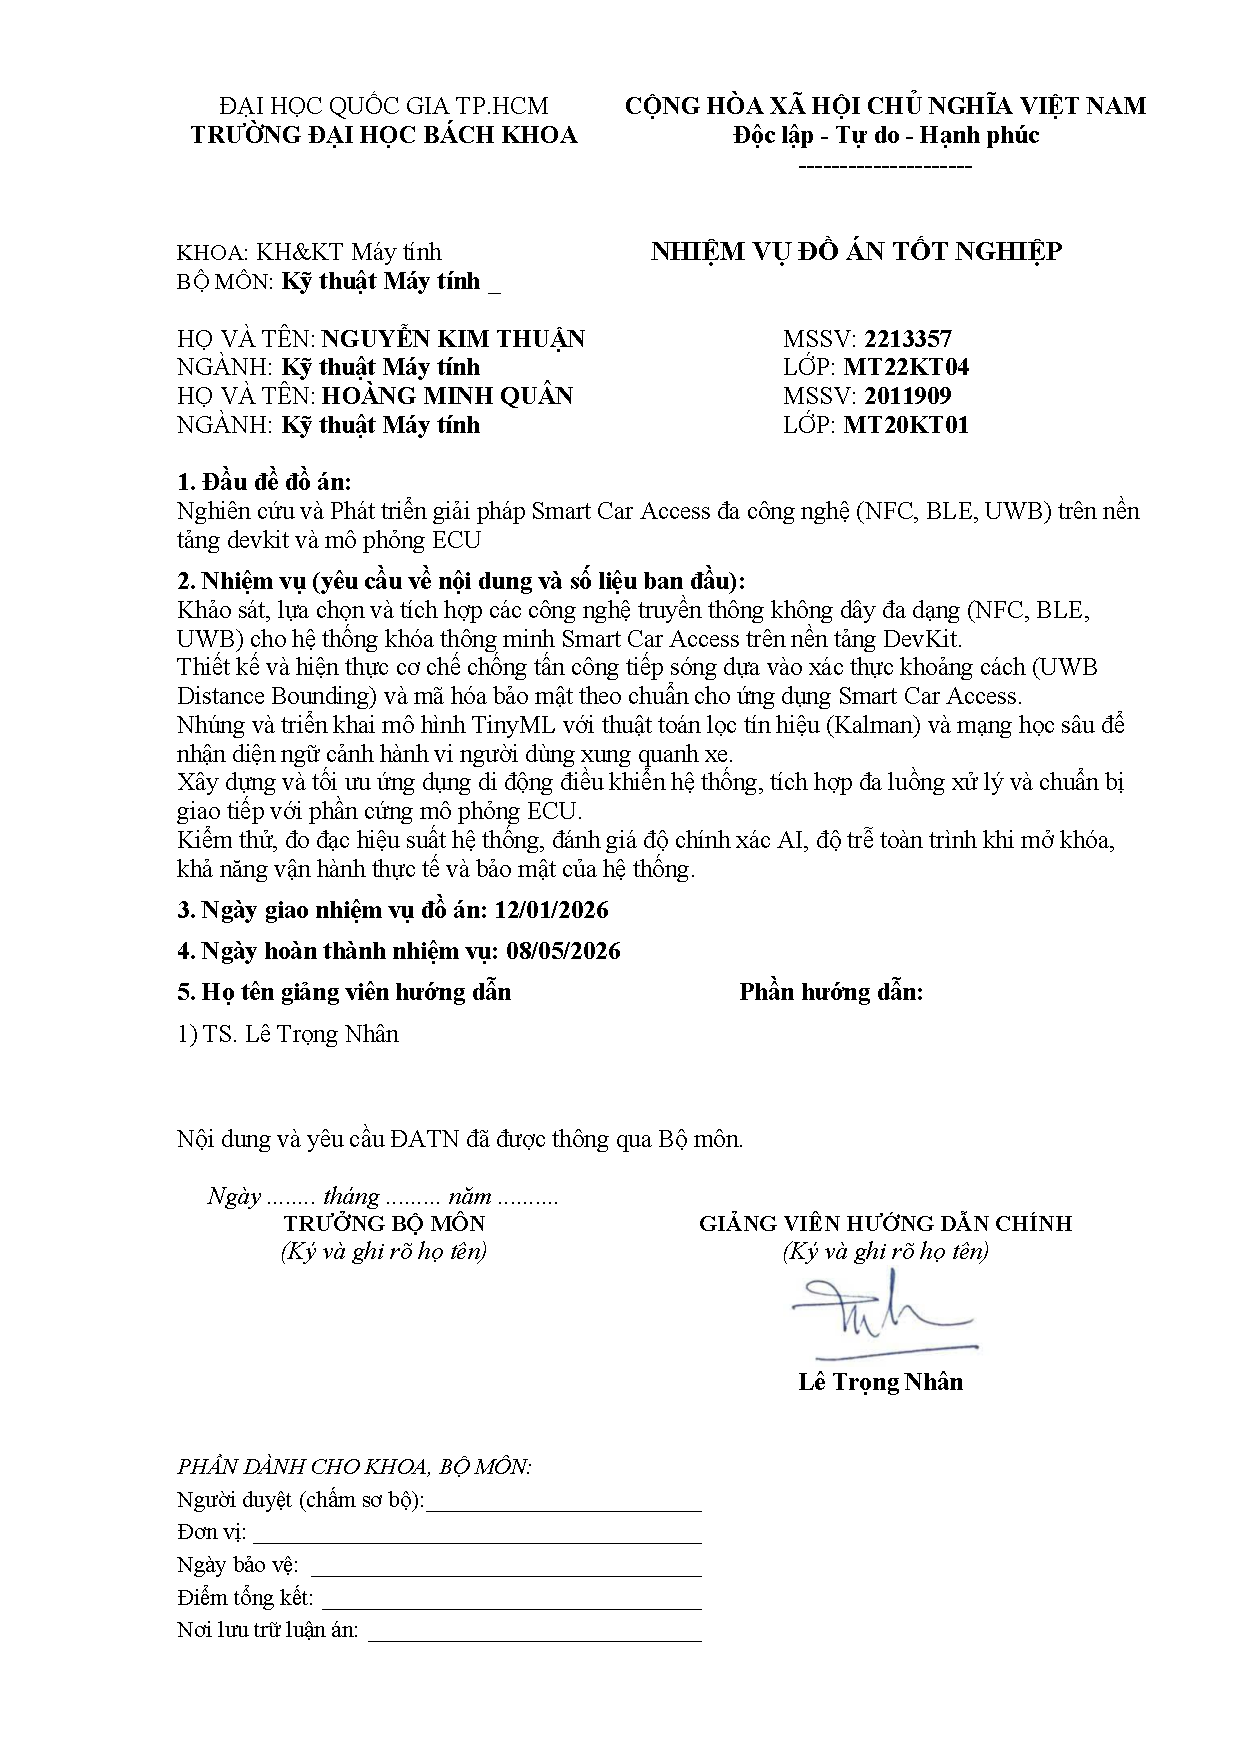
\includepdf[pages=1,pagecommand={},width=\paperwidth,height=\paperheight]{pdf files/Nv_signed.pdf}
% \clearpage


% %============================phieu huong dan=========================
% \newpage
% 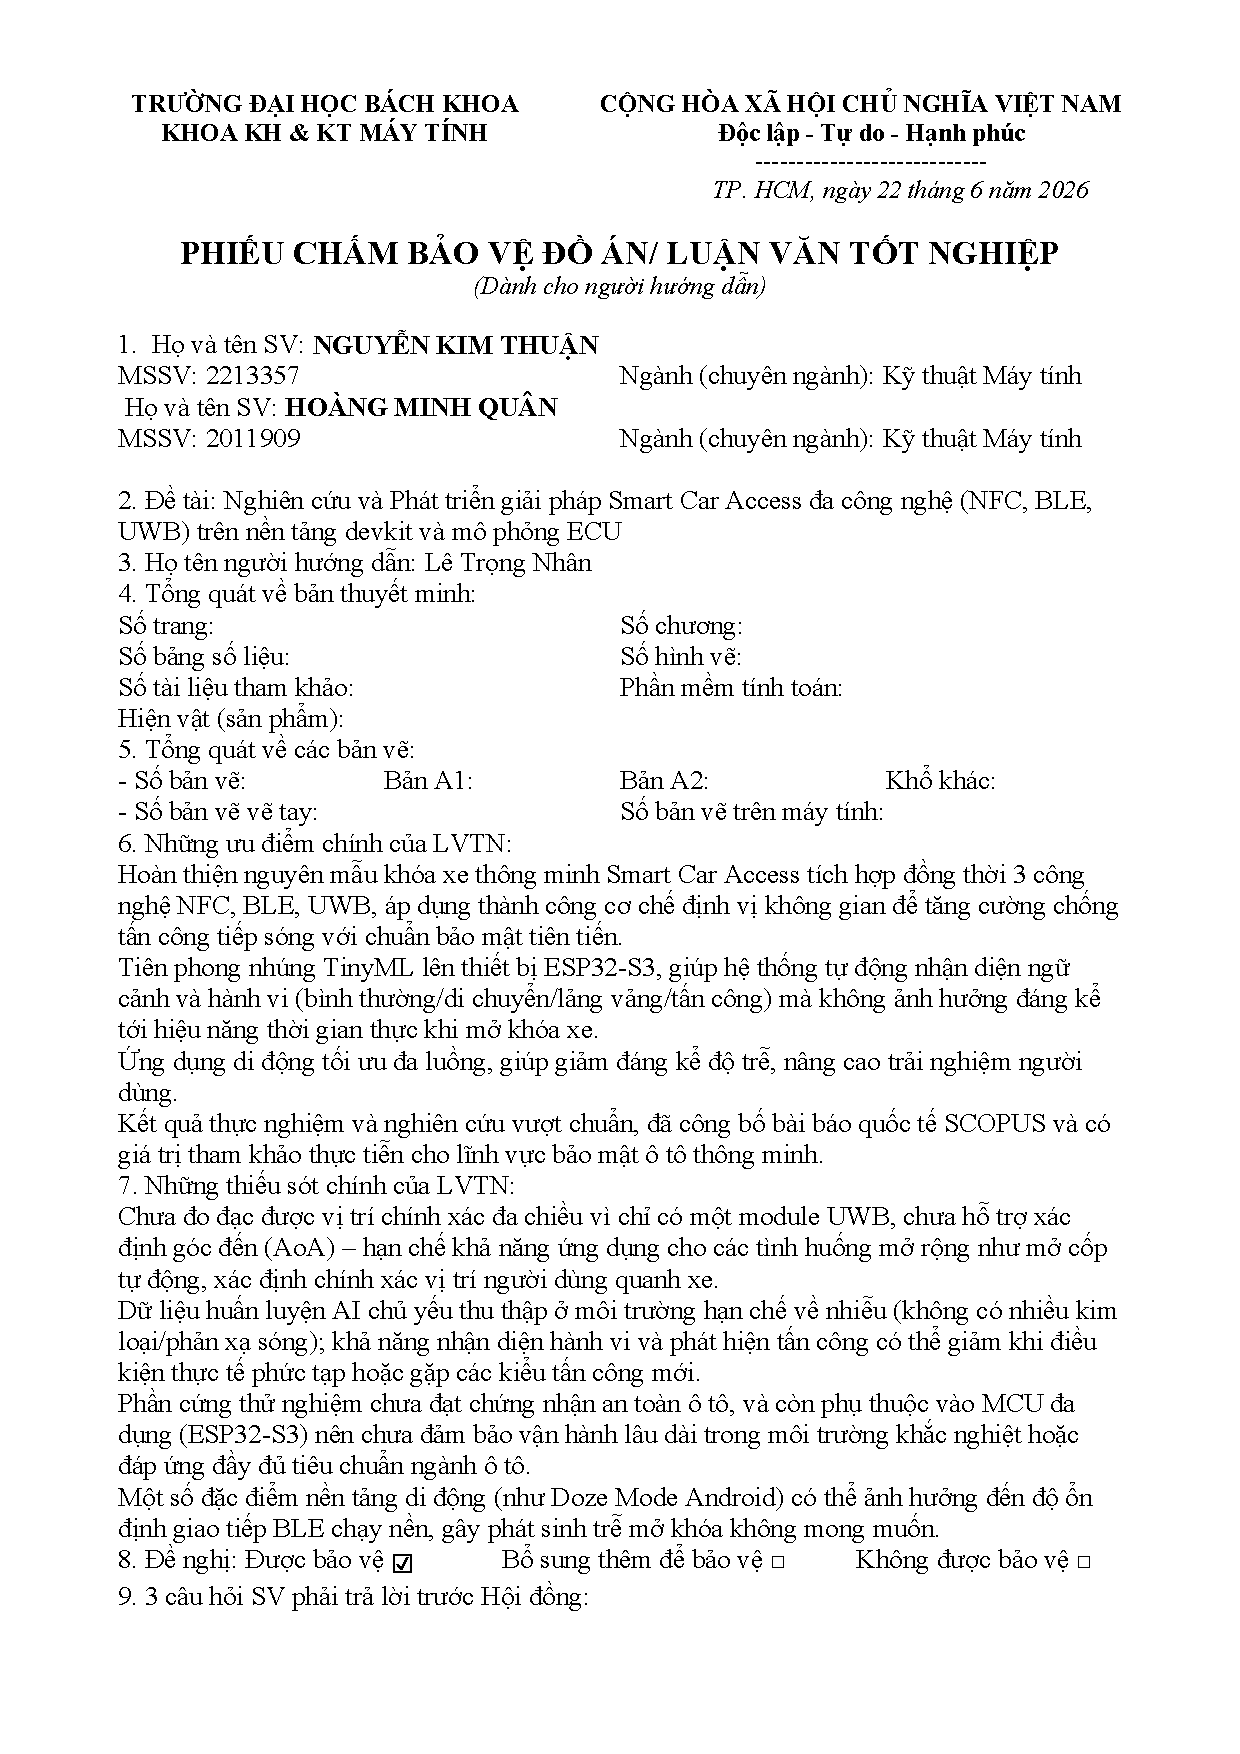
\includepdf[pages=1,pagecommand={},width=\paperwidth,height=\paperheight]{pdf files/Hd_signed.pdf}
% \clearpage

% \newpage
% \includepdf[pages=2,pagecommand={},width=\paperwidth,height=\paperheight]{pdf files/Hd_signed.pdf}
% \clearpage


% %============================phieu phan bien=========================
% \newpage
% 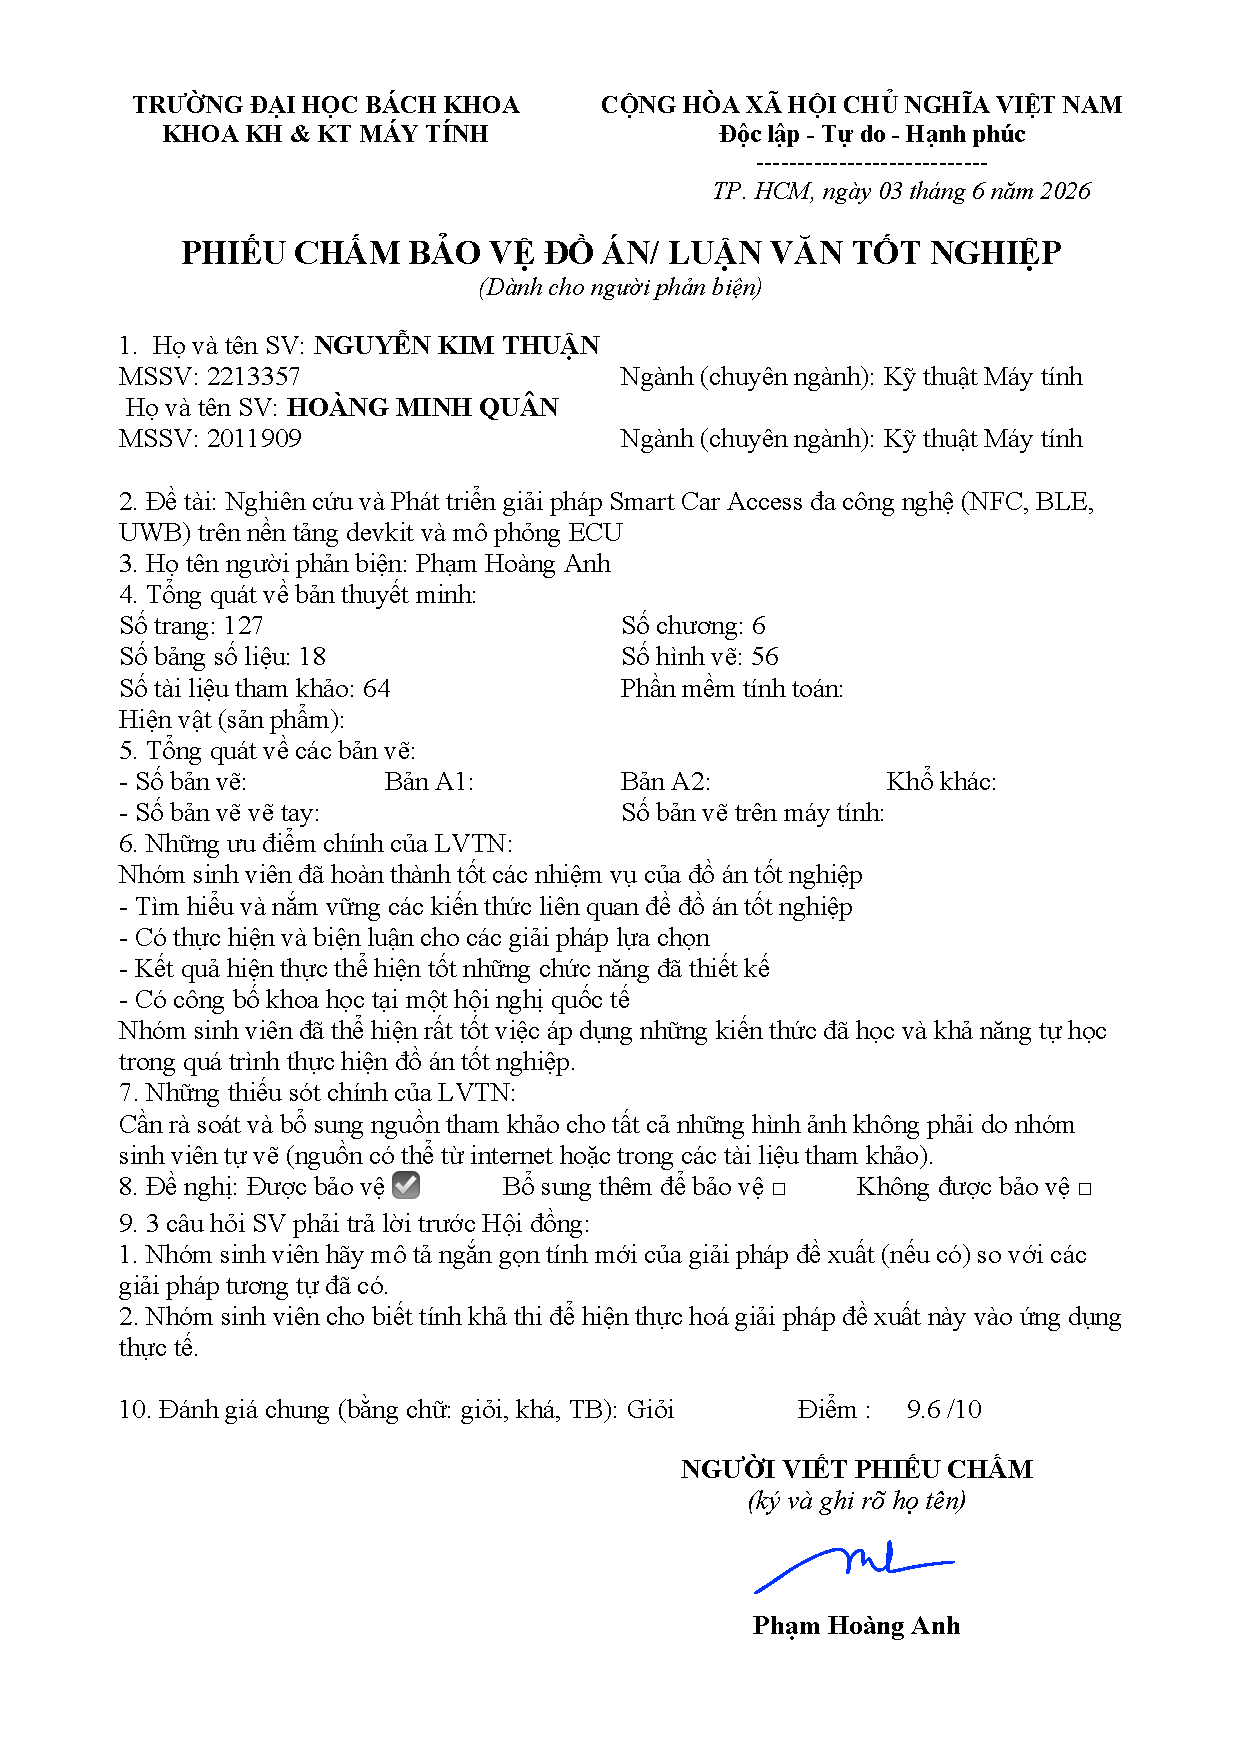
\includepdf[pages=1,pagecommand={},width=\paperwidth,height=\paperheight]{pdf files/PB_signed.pdf}
% \clearpage

\end{titlepage}
\restoregeometry

\clearpage
\phantomsection
\addcontentsline{toc}{chapter}{LỜI CAM ĐOAN}
\section*{\MakeUppercase{LỜI CAM ĐOAN}}
\begin{quotation}
Tôi xin cam đoan toàn bộ nội dung và kết quả của đề tài “Nghiên cứu và Phát triển hệ thống Định vị đa điểm (Multi-anchor) và Nhận diện ý định hành vi dựa trên TinyML cho giải pháp Smart Car Access” là sản phẩm nghiên cứu, tìm hiểu và phát triển của riêng tôi dưới sự hướng dẫn khoa học của TS. Lê Trọng Nhân.

Các kết quả, số liệu và mã nguồn được trình bày trong báo cáo là hoàn toàn trung thực, phản ánh đúng kết quả thực nghiệm của tôi và chưa từng được công bố trong bất kỳ công trình nghiên cứu nào khác của các tác giả khác hay tại các cơ sở đào tạo khác.

Trong quá trình thực hiện đề tài, tôi có tham khảo và kế thừa các thành tựu khoa học, tài liệu, sách báo và các trang web chuyên ngành. Tất cả các nguồn tài liệu tham khảo này đều được trích dẫn đầy đủ, rõ ràng.

Nếu phát hiện có bất kỳ sự gian lận, sao chép không hợp lệ hay vi phạm các nguyên tắc về liêm chính học thuật, tôi xin chịu hoàn toàn trách nhiệm và chấp nhận mọi hình thức kỷ luật theo quy định.
\end{quotation}

\begin{flushright}
\begin{tabular}{c}
Tp. Hồ Chí Minh, tháng 09/2026\\
\textbf{Sinh viên thực hiện}\\
Võ Thành Nhân
\end{tabular}
\end{flushright}


\clearpage
\phantomsection
\addcontentsline{toc}{chapter}{LỜI CẢM ƠN}
\section*{\MakeUppercase{LỜI CẢM ƠN}}
\begin{quotation}
Trong suốt quá trình thực hiện luận văn tốt nghiệp với đề tài: “Nghiên cứu và Phát triển hệ thống Định vị đa điểm (Multi-anchor) và Nhận diện ý định hành vi dựa trên TinyML cho giải pháp Smart Car Access”, em đã có cơ hội kế thừa và phát triển từ đồ án chuyên ngành trước đó. Đây là một quá trình đòi hỏi sự đầu tư nghiêm túc cả về kiến thức chuyên môn lẫn kỹ năng nghiên cứu, qua đó giúp em từng bước hoàn thiện năng lực học thuật và thực tiễn. Để hoàn thành luận văn này, bên cạnh sự nỗ lực của bản thân, em đã nhận được rất nhiều sự hỗ trợ quý báu từ quý thầy cô, gia đình và bạn bè.
\singlespacing 
Trước hết, em xin bày tỏ lòng biết ơn chân thành đến toàn thể quý thầy cô giảng viên Trường \textit{Đại học Bách Khoa - Đại học Quốc gia Thành phố Hồ Chí Minh}, những người đã tận tâm giảng dạy, truyền đạt kiến thức và định hướng tư duy nghiên cứu trong suốt quá trình học tập. Những kiến thức nền tảng từ các môn học cơ sở đến chuyên ngành chính là tiền đề quan trọng giúp em có thể tiếp cận, phát triển và hoàn thiện đề tài luận văn này.
\singlespacing 
Đặc biệt, em xin gửi lời cảm ơn sâu sắc đến \textbf{TS. Lê Trọng Nhân}, người đã trực tiếp hướng dẫn và đồng hành cùng em trong suốt quá trình thực hiện luận văn. Thầy đã tận tình chỉ bảo và đóng góp nhiều ý kiến chuyên môn quý giá, giúp em định hướng rõ ràng hơn trong nghiên cứu cũng như hoàn thiện nội dung luận văn một cách khoa học và chặt chẽ. Em cũng trân trọng cảm ơn hội nghị IAAA 2026 đã ghi nhận và chấp nhận bài báo liên quan đến đề tài, tạo thêm động lực để em tiếp tục hoàn thiện nghiên cứu.
\singlespacing 
Bên cạnh đó, em xin chân thành cảm ơn gia đình đã luôn là chỗ dựa vững chắc, động viên và hỗ trợ em trong suốt quá trình học tập và nghiên cứu. Đồng thời, em cũng cảm ơn bạn bè và đồng nghiệp đã luôn đồng hành, chia sẻ kinh nghiệm và hỗ trợ lẫn nhau trong quá trình thực hiện luận văn. 
\singlespacing 
Mặc dù đã nỗ lực hoàn thiện luận văn một cách tốt nhất, song do hạn chế về thời gian và kinh nghiệm nghiên cứu, luận văn khó tránh khỏi những thiếu sót. Em rất mong nhận được những ý kiến đóng góp quý báu từ quý thầy cô để có thể tiếp tục hoàn thiện và phát triển đề tài trong tương lai.

\singlespacing
Xin chân thành cảm ơn!

\begin{flushright}
\begin{tabular}{c}
Tp. Hồ Chí Minh, tháng 09/2026\\
\textbf{Sinh viên thực hiện}\\
Võ Thành Nhân
\end{tabular}
\end{flushright}

\end{quotation}



% ==========================
% TÓM TẮT
% ==========================
\clearpage
\phantomsection
\addcontentsline{toc}{chapter}{TÓM TẮT}
\section*{\MakeUppercase{TÓM TẮT}}

Đề tài \textbf{``Nghiên cứu và Phát triển hệ thống Định vị đa điểm (Multi-anchor) và Nhận diện ý định hành vi dựa trên TinyML cho giải pháp Smart Car Access''} kế thừa và phát triển từ đồ án chuyên ngành về hệ thống truy cập xe không chìa khóa, được thực hiện theo hai giai đoạn.

\textbf{Giai đoạn 1 (Stage 1)} xây dựng nền tảng xác thực tuân thủ chuẩn \textit{Car Connectivity Consortium (CCC)}: \textbf{NFC} đảm nhận cấp quyền vật lý tầm gần (Provisioning), \textbf{BLE} thực hiện xác thực tầm trung (Authentication) với các thuật toán mật mã HMAC-SHA256 và AES-128-GCM, được điều phối bởi máy trạng thái hữu hạn (FSM) trên vi điều khiển ESP32-S3 kết hợp ứng dụng di động Flutter.

\textbf{Giai đoạn 2 (Stage 2)} là trọng tâm của luận văn, nâng cấp năng lực định vị và ra quyết định: hệ thống bố trí \textbf{ba mỏ neo UWB} cố định trên xe, thu thập đồng thời ba khoảng cách và giải tọa độ phẳng $(x, y)$ của người dùng bằng \textbf{Trilateration}, sau đó hợp nhất quỹ đạo bằng \textbf{bộ lọc Kalman mở rộng (EKF)} để ước lượng cả vị trí lẫn vận tốc $(x, y, v_x, v_y)$. Tọa độ này được đối chiếu với các vùng kích hoạt (geofencing) và kết hợp mô hình \textbf{TinyML} (mạng tích chập 1D) nhúng trên thiết bị biên để nhận diện ý định hành vi (Approach, Seated, Leave, Passing) nhằm đưa ra quyết định chính xác.

Kết quả thực nghiệm cho thấy hệ thống đạt khả năng mở khóa ổn định, an toàn và nâng cao đáng kể so với các phương pháp chỉ dựa trên BLE hoặc đo khoảng cách đơn mỏ neo, tạo tiền đề phát triển thành một hệ thống hoàn chỉnh trong môi trường thực tế.

\par\vspace{2em}
\textbf{\underline{Các từ khóa}}: Keyless Entry, CCC, NFC, BLE, UWB, Multi-anchor, Trilateration, Kalman Filter, TinyML, HMAC-SHA256, AES-128-GCM, ESP32-S3, Automotive Security, FSM.


% ==========================
% MỤC LỤC
% ==========================
\newpage
\tableofcontents
% \newpage

% ==========================
% DANH MỤC HÌNH VẼ
% ==========================
\cleardoublepage
\phantomsection
\addcontentsline{toc}{chapter}{DANH SÁCH HÌNH ẢNH}
\listoffigures
\newpage

% ==========================
% DANH MỤC BẢNG
% ==========================
\cleardoublepage
\phantomsection
\addcontentsline{toc}{chapter}{DANH SÁCH BẢNG}
\listoftables
\newpage

% ==========================
% DANH MỤC TỪ VIẾT TẮT
% ==========================
\chapter*{\MakeUppercase{DANH MỤC TỪ VIẾT TẮT}}
\addcontentsline{toc}{chapter}{DANH MỤC TỪ VIẾT TẮT}

\begin{longtable}{p{3cm} p{11cm}}
\textbf{Viết tắt} & \textbf{Diễn giải} \\
\hline
\endhead

ADAS & Advanced Driver Assistance Systems \\
AES-GCM & Advanced Encryption Standard – Galois/Counter Mode \\
API & Application Programming Interface \\
BLE & Bluetooth Low Energy \\
CCC & Car Connectivity Consortium \\
DS-TWR & Double-Sided Two-Way Ranging \\
ECU & Electronic Control Unit \\
EKF & Extended Kalman Filter \\
ESP32-S3 & Espressif ESP32-S3 Microcontroller \\
EV & Electric Vehicle \\
FSM & Finite State Machine \\
GATT & Generic Attribute Profile \\
GDOP & Geometric Dilution of Precision \\
GPIO & General Purpose Input/Output \\
HMAC & Hash-based Message Authentication Code \\
HMAC-SHA256 & HMAC using SHA-256 \\
IEC & International Electrotechnical Commission \\
ISO & International Organization for Standardization \\
IoT & Internet of Things \\
MAC & Message Authentication Code \\
MaaS & Mobility-as-a-Service \\
MITM & Man-in-the-Middle \\
NFC & Near Field Communication \\
NIST & National Institute of Standards and Technology \\
PKE & Passive Keyless Entry \\
RF & Radio Frequency \\
RFID & Radio Frequency Identification \\
RKE & Remote Keyless Entry \\
RMS & Root Mean Square \\
SDV & Software-Defined Vehicles \\
STS & Scrambled Timestamp Sequence \\
ToF & Time of Flight \\
UART & Universal Asynchronous Receiver-Transmitter \\
UCI & UWB Command Interface \\
UWB & Ultra-Wideband \\
V2X & Vehicle-to-Everything \\
\end{longtable}

\newpage


% ==========================
% NỘI DUNG CHÍNH
% ==========================
\chapter{\MakeUppercase{Giới thiệu tổng quan}} 
\section{Bối cảnh và động lực phát triển}

\subsection{Xu hướng phát triển xe thông minh}

Trong kỷ nguyên chuyển đổi số và kết nối vạn vật (IoT), ngành công nghiệp ô tô toàn cầu đang trải qua một cuộc cách mạng mạnh mẽ từ các phương tiện cơ khí truyền thống sang xe thông minh (Smart Vehicles) và xe được định nghĩa bởi phần mềm (Software-Defined Vehicles - SDV). Theo báo cáo của McKinsey \& Company (2023)\cite{mckinsey2023}, thị trường xe thông minh toàn cầu dự kiến đạt 556 tỷ USD vào năm 2026 với tốc độ tăng trưởng hàng năm 12.5\%. Xu hướng này được thúc đẩy bởi ba yếu tố chính:

\begin{enumerate}
    \item Connectivity (Kết nối): Các phương tiện hiện đại được tích hợp khả năng kết nối Internet và giao tiếp V2X (Vehicle-to-Everything), cho phép trao đổi dữ liệu với hạ tầng giao thông, các phương tiện khác và điện thoại thông minh của người dùng.
    
    \item Electrification (Điện khí hóa): Sự bùng nổ của xe điện (EV) và xe Hybrid đòi hỏi các hệ thống điện tử phức tạp hơn để quản lý năng lượng, sạc pin và tối ưu hóa hiệu suất.
    
    \item Autonomous Driving (Tự lái): Các công nghệ ADAS (Advanced Driver Assistance Systems) và Autonomous Driving yêu cầu hàng trăm cảm biến, ECU và khả năng xử lý dữ liệu thời gian thực.
\end{enumerate}

\begin{figure}[htbp]
\centering
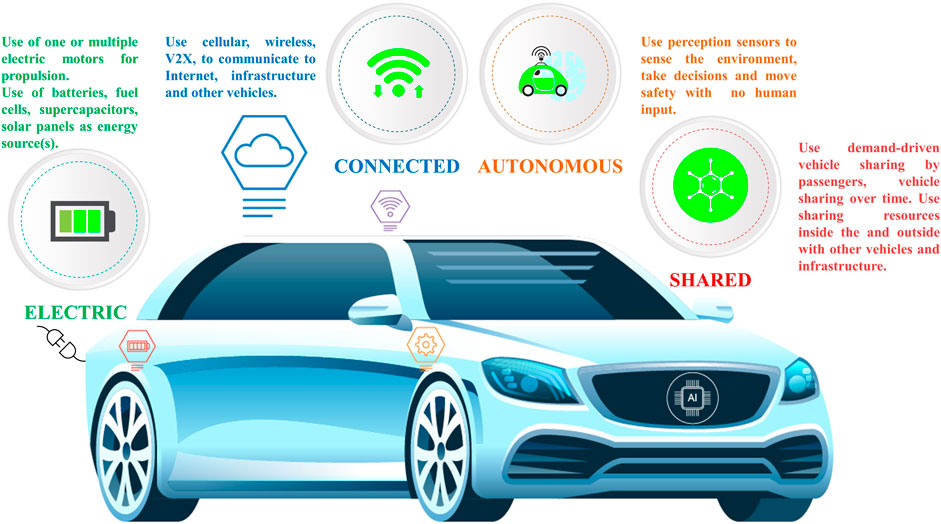
\includegraphics[width=0.8\textwidth]{image/section2/car.jpg}
\caption[Hệ sinh thái xe kết nối (Connected Vehicle Ecosystem)]{Hệ sinh thái xe kết nối (Connected Vehicle Ecosystem) (\textbf{Nguồn:} \href{https://www.frontiersin.org/journals/future-transportation/articles/10.3389/ffutr.2021.688482/full}{Frontiers})}
\label{fig:connected_vehicle}
\end{figure}

Trong bối cảnh này, hệ thống truy cập xe thông minh (Smart Car Access System) đã trở thành một trong những tính năng quan trọng nhất, không chỉ nâng cao trải nghiệm người dùng mà còn là nền tảng cho các dịch vụ Mobility-as-a-Service (MaaS) và Car Sharing trong tương lai. Xu hướng \textbf{"chìa khóa kỹ thuật số"} (Digital Key) đang dần thay thế các loại chìa khóa vật lý và Remote Keyless Entry (RKE) truyền thống, cho phép người dùng mở khóa, khởi động xe và cá nhân hóa cài đặt chỉ bằng điện thoại thông minh.

Các hãng ô tô hàng đầu như Tesla, BMW, Mercedes-Benz, và Hyundai đã triển khai các giải pháp Digital Key sử dụng công nghệ Bluetooth Low Energy (BLE), Near Field Communication (NFC) và Ultra-Wideband (UWB). Car Connectivity Consortium (CCC) - tổ chức gồm các thành viên như Apple, Samsung, Audi, BMW, General Motors - đã phát hành chuẩn Digital Key Release 3.0 vào năm 2021 \cite{ccc_digikey3}, sử dụng UWB để chống tấn công relay và đảm bảo secure ranging với độ chính xác centimet.

\begin{figure}[H]
\centering
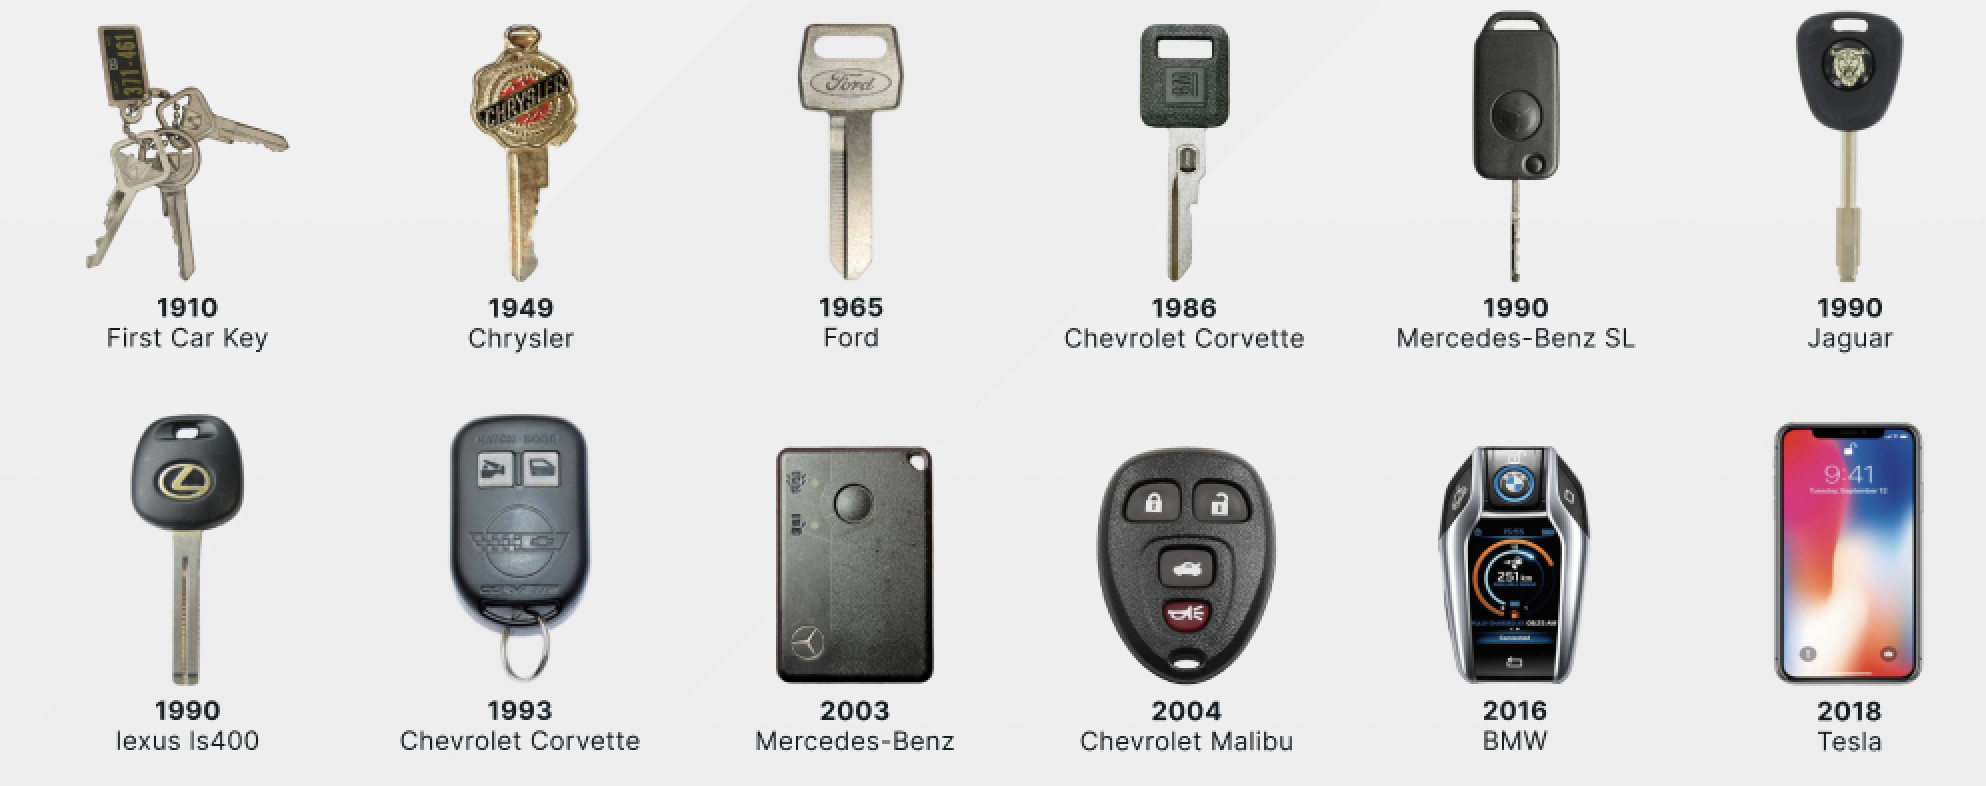
\includegraphics[width=0.8\textwidth]{image/section2/car3.png}
\caption{Công nghệ chìa khóa qua các thời kì}
\label{fig:digital_key_evolution}
\end{figure}

\subsection{Vấn đề bảo mật của các hệ thống Keyless Entry truyền thống}
Mặc dù công nghệ Keyless Entry mang lại sự tiện lợi vượt trội, các hệ thống truyền thống đang đối mặt với nhiều thách thức nghiêm trọng về bảo mật:
\begin{enumerate}
    \item \textbf{Tấn công chuyển tiếp (Relay Attack)} 
    
    Đây là mối đe dọa lớn nhất đối với hệ thống Passive Keyless Entry (PKE). Kẻ tấn công sử dụng hai thiết bị để khuếch đại và chuyển tiếp tín hiệu giữa chìa khóa (hoặc điện thoại) và xe, tạo ảo giác rằng chìa khóa đang ở gần xe. Nghiên cứu của Francillon et al. (2011) \cite{francillon2011relay} đã chứng minh hầu hết các xe sử dụng PKE đều dễ bị tấn công này, bao gồm cả các thương hiệu cao cấp như Audi A6, BMW X5, và Range Rover Sport.

    \begin{figure}[H]
    \centering
    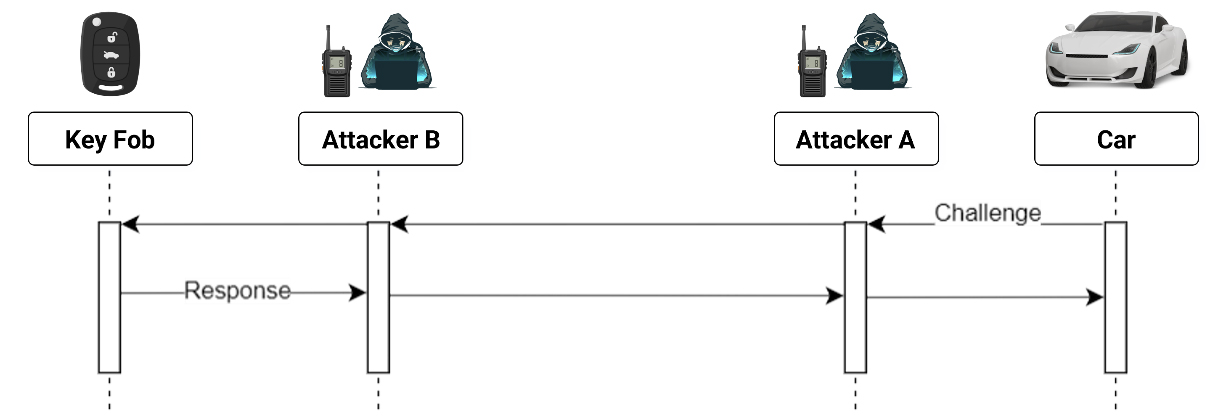
\includegraphics[width=0.85\textwidth]{image/section2/car2.jpg}
    \caption[Sơ đồ minh họa tấn công chuyển tiếp (Relay Attack) trên hệ thống Keyless Entry]{Sơ đồ minh họa tấn công chuyển tiếp (Relay Attack) trên hệ thống Keyless Entry (\textbf{Nguồn:} \href{https://www.automotiveworld.com/articles/mitigating-vulnerabilities-in-keyless-entry-systems/}{Automotive World})}
    \label{fig:relay_attack}
    \end{figure}

    Năm 2021, nhóm nghiên cứu của Lennert Wouters tại KU Leuven \cite{wouters2021tesla} đã công bố lỗ hổng bảo mật trên hệ thống BLE-only của Tesla Model 3 và Model Y, cho phép kẻ tấn công mở khóa và khởi động xe bằng cách relay các gói tin BLE. Tesla đã phải phát hành bản vá khẩn cấp để giảm thiểu rủi ro.
    
    \item \textbf{Tấn công phát lại (Replay Attack)} 
    
    Kẻ tấn công ghi lại tín hiệu mở khóa hợp lệ từ chìa khóa của người dùng và phát lại tín hiệu đó sau này để chiếm quyền kiểm soát. Mặc dù công nghệ mã hóa thay đổi (Rolling Code) đã được áp dụng, nhiều hệ thống vẫn tồn tại lỗ hổng do việc hiện thực hóa giao thức không đúng cách hoặc thiếu cơ chế xác thực thách thức - phản hồi (Challenge-Response) đủ mạnh.
    
    \item \textbf{Sao chép và giả mạo chìa khóa (Key Cloning \& Brute Force)} 
    
    Đối với các hệ thống có không gian khóa nhỏ hoặc không giới hạn tốc độ thử, kẻ tấn công có thể dò tìm mã khóa (Brute Force). Ngoài ra, sự phổ biến của các thiết bị phần cứng mã nguồn mở như Proxmark3 hay Flipper Zero cho phép sao chép dễ dàng các thẻ từ (RFID) hoặc Key Fob có độ bảo mật thấp.
    
    \item \textbf{Nghe lén dữ liệu (Eavesdropping)}
    
    Nếu giao thức truyền thông không đảm bảo tính bí mật chuyển tiếp (Forward Secrecy) và mã hóa mạnh, thông tin định danh nhạy cảm truyền qua sóng vô tuyến có thể bị kẻ gian thu thập và giải mã, tạo tiền đề cho các cuộc tấn công giả mạo về sau.
\end{enumerate}


\subsection{Các giải pháp Digital Key}

Để giải quyết các vấn đề bảo mật trên, các hãng ô tô đã phát triển nhiều giải pháp Digital Key khác nhau:
\begin{enumerate}
    \item \textbf{Tesla Model 3/Y}
    
    Tesla sử dụng kiến trúc đơn giản chỉ dựa trên BLE cho cả cấp phát khoá (Provisioning) và xác thực (Authentication). Ưu điểm của cách tiếp cận này là không cần phần cứng NFC, cho phép khoảng cách hoạt động xa (50--100\,m), và tích hợp sẵn với ứng dụng Tesla mobile app. Tuy nhiên, như đã đề cập, giải pháp này dễ bị tấn công chuyển tiếp (Relay Attack) do không có cơ chế xác minh khoảng cách vật lý. Chỉ số RSSI (Received Signal Strength Indicator) của BLE không đủ chính xác để phân biệt khoảng cách thực sự, với sai số có thể lên đến 10--15\%. \cite{wouters2021tesla,gomez2012overview,heydon2013bluetooth}

    \item \textbf{BMW Digital Key} 
    
    BMW là một trong những hãng đầu tiên triển khai Digital Key Release 3.0 của Car Connectivity Consortium \cite{ccc_digikey3}, sử dụng kết hợp cả ba công nghệ: NFC cho cấp phát khóa (chạm điện thoại vào B-pillar), BLE cho phát hiện thiết bị, và \textbf{UWB cho đo khoảng cách an toàn}. UWB có khả năng đo khoảng cách với độ chính xác $<10$\,cm và cơ chế đo thời gian bay (time-of-flight measurement) giúp chống lại tấn công relay một cách hiệu quả \cite{ieee802154z,sidorenko2020accurate}. Tuy nhiên, giải pháp này yêu cầu phần cứng đắt tiền (chip UWB khoảng \$50), chỉ hỗ trợ một số mẫu iPhone mới nhất (iPhone~11 trở lên), và sử dụng giao thức độc quyền của BMW.

    \item \textbf{NXP CarKey Solution} 
    
    NXP Semiconductors cung cấp giải pháp CarKey dựa trên NFC Forum Type~4 Tag và Secure Element (SE) để lưu trữ khóa số \cite{iso14443,iso7816}. Ưu điểm của giải pháp này là mức độ bảo mật phần cứng cao (chip SE có khả năng chống can thiệp vật lý), tuân thủ tiêu chuẩn Global Platform, và hỗ trợ nhiều điện thoại cùng lúc. Nhược điểm là chi phí cao do cần chip SE (khoảng \$5--10 cho mỗi đơn vị), luồng cấp phát khóa phức tạp, và phụ thuộc nhà cung cấp (Vendor lock-in) vào hệ sinh thái của NXP.

\end{enumerate}


Từ phân tích các giải pháp hiện có, có thể thấy tồn tại một trade-off giữa bảo mật, chi phí và tính khả thi triển khai:

\begin{itemize}
    \item Các giải pháp BLE (Tesla) có chi phí thấp nhưng bảo mật chưa tối ưu
    \item Các giải pháp NFC + UWB (BMW) có bảo mật cao nhưng yêu cầu phần cứng đắt đỏ và hỗ trợ thiết bị hạn chế
    \item Các giải pháp dựa trên SE (NXP) có bảo mật phần cứng tốt nhưng chi phí cao và phức tạp
\end{itemize}

\begin{figure}[H]
\centering
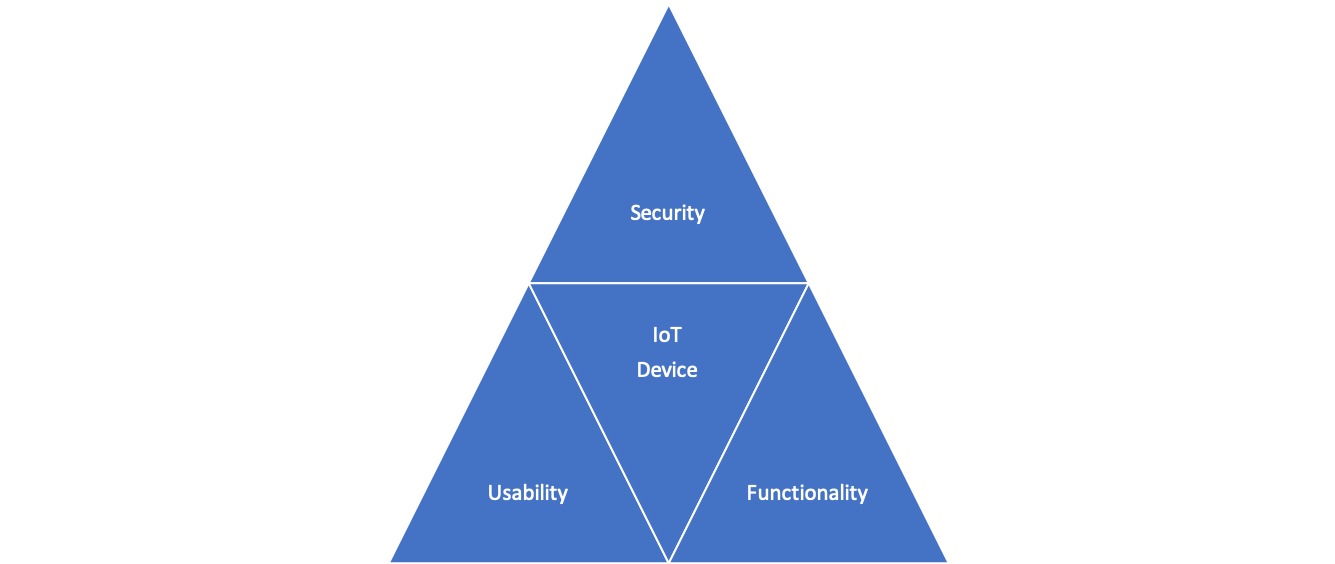
\includegraphics[width=0.75\textwidth]{image/section2/car4.png}
\caption[Trade-off giữa bảo mật, chi phí và tính khả thi của các giải pháp Digital Key]{Trade-off giữa bảo mật, chi phí và tính khả thi của các giải pháp Digital Key}
\label{fig:tradeoff}
\end{figure}

Đối với thị trường Việt Nam và các nước đang phát triển, nhu cầu về một giải pháp cân bằng giữa bảo mật và chi phí là rất cấp thiết. Các yêu cầu cụ thể bao gồm:

\begin{enumerate}
    \item \textbf{Bảo mật cao:} Tuân thủ các chuẩn mật mã quốc tế (NIST) \cite{nist_ecdh, fips186}, chống được Replay Attack và MITM Attack. Giảm thiểu Relay Attack mức độ tối đa có thể với công nghệ NFC + BLE và UWB trong tương lai.
    
    \item \textbf{Chi phí hợp lý:} Giải pháp sử dụng phần cứng sẵn có, các mã nguồn mở (open-source software stack), và không yêu cầu các chip chuyên dụng (SE, UWB) trong giai đoạn thử nghiệm.

    \item \textbf{Dễ triển khai:} Quy trình cấp phát khoá ban đầu đơn giản (NFC tap), hỗ trợ đa nền tảng (iOS và Android), và có khả năng tích hợp với các hệ thống ECU ô tô trong tương lai.

    \item \textbf{Khả năng nghiên cứu:} Mã nguồn mở, tài liệu hỗ trợ đầy đủ, có thể dùng làm tài liệu học tập cho sinh viên và kỹ sư trong nước.
\end{enumerate}

\section{Bối cảnh thị trường ô tô Việt Nam}

Tại Việt Nam, thị trường ô tô đang có tốc độ tăng trưởng ấn tượng với doanh số xe du lịch đạt hơn 300,000 chiếc trong năm 2023 (theo VAMA \cite{vama2023}). Người tiêu dùng ngày càng khắt khe về các tính năng công nghệ và tiện nghi, đặc biệt là thế hệ trẻ quen với smartphone và các thiết bị IoT. Chính phủ cũng đang đẩy mạnh đầu tư vào nghiên cứu và phát triển công nghiệp ô tô nội địa, với mục tiêu giảm phụ thuộc vào công nghệ nhập khẩu và tham gia sâu hơn vào chuỗi giá trị toàn cầu.

\begin{figure}[H]
\centering
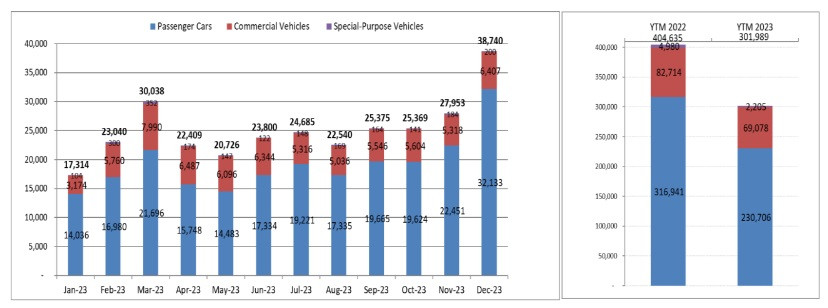
\includegraphics[width=0.8\textwidth]{image/section2/car5.jpg}
\caption[Tăng trưởng thị trường ô tô Việt Nam (Nguồn: VAMA 2023)]{Tăng trưởng thị trường ô tô Việt Nam (Nguồn: VAMA 2023) \cite{vama2023}}
\label{fig:vietnam_market}
\end{figure}

Việc nghiên cứu các giải pháp Smart Car Access trên nền tảng vi điều khiển và mô phỏng ECU không chỉ phù hợp với định hướng phát triển công nghệ quốc gia mà còn là bước đệm quan trọng để:

\begin{itemize}
    \item Kỹ sư Việt Nam tiếp cận và làm chủ các công nghệ lõi trong Automotive Security
    \item Xây dựng năng lực R\&D cho các doanh nghiệp Tier-2, Tier-3 trong chuỗi cung ứng ô tô
    \item Cung cấp giải pháp Aftermarket cho các xe đã qua sử dụng tại thị trường nội địa
    \item Tạo nền tảng cho các Startup công nghệ ô tô và IoT trong nước
\end{itemize}

Đề tài này hướng đến việc phát triển một \textit{\textbf{tài liệu tham khảo}} mã nguồn mở cho hệ thống truy cập xe thông minh (Smart Car Access) sử dụng kiến trúc kết hợp NFC--BLE, với khả năng chuyển đổi sang các ECU ô tô và mở rộng tích hợp UWB. Giải pháp được xây dựng dựa trên các chuẩn quốc tế (NIST, ISO) \cite{nist_ecdh, iso14443}, đồng thời tối ưu hoá cho chi phí nghiên cứu và triển khai tại các thị trường đang phát triển.

\section{Yêu cầu và mục tiêu đề tài}

\subsection{Yêu cầu đề tài}

Đề tài tập trung vào việc nghiên cứu và triển khai một hệ thống truy cập xe thông minh (Smart Car Access) sử dụng công nghệ truyền thông không dây hiện đại trên nền tự vi điều khiển. Hệ thống có chức năng chính là xác thực người dùng, thiết lập kết nối an toàn và điều khiển truy cập xe tự động, định hướng tuân thủ theo các tiêu chuẩn công nghiệp hiện hành. Đề tài yêu cầu đảm bảo các tiêu chí sau:

\begin{enumerate}
    \item \textbf{Tích hợp công nghệ truyền thông không dây:}
    
    Hệ thống phần cứng phải tích hợp thành công và đồng bộ các module giao tiếp \textbf{NFC (Near Field Communication)}, \textbf{BLE (Bluetooth Low Energy)} và \textbf{UWB (Ultra-Wideband)}. NFC đảm nhiệm vai trò đăng ký thiết bị ban đầu (Provisioning) với yêu cầu về tiếp xúc vật lý ở khoảng cách gần, nhằm đảm bảo tính bảo mật cốt lõi trong giai đoạn thiết lập. BLE thực hiện quá trình thiết lập kênh liên lạc an toàn và xác thực (Authentication) với phạm vi hoạt động rộng hơn. Đặc biệt, công nghệ UWB đã được hiện thực hóa để đóng vai trò then chốt trong việc đo lường và xác minh khoảng cách an toàn (Secure Distance Verification), giúp ngăn chặn triệt để các rủi ro giả mạo vị trí.

    \item \textbf{Phát triển ứng dụng Smart Car:}
    
    Xây dựng ứng dụng di động đa nền tảng (Cross-platform) đóng vai trò như một ``chìa khóa kỹ thuật số'' (Digital Key). Ứng dụng cần có khả năng giao tiếp liên tục với bộ điều khiển phương tiện thông qua nền tảng NFC/BLE/UWB, đồng thời hiển thị trạng thái kết nối và trạng thái xe (locked/unlocked). Hệ thống hỗ trợ quản lý xác thực người dùng thông qua Firebase và lưu trữ các khóa mật mã (Cryptographic Keys) một cách an toàn trên thiết bị.

    \item \textbf{Xây dựng giao thức bảo mật:}
    
    Hệ thống cần triển khai các giao thức mật mã tuân thủ các chuẩn quốc tế (NIST) \cite{nist_ecdh, fips186} nhằm đảm bảo mức độ bảo mật cao. Giải pháp sử dụng Elliptic Curve Cryptography (ECC) cho quá trình trao đổi khóa (Key Exchange) và chữ ký số (Digital Signature), kết hợp với mã hóa đối xứng (Symmetric encryption) cho truyền tải dữ liệu. Cơ chế xác thực hai chiều (Mutual authentication) được duy trì để chống lại các tấn công trung gian (Man-in-the-Middle -- MITM attack). Để củng cố toàn diện, giao thức bảo mật thiết lập sự ràng buộc mật mã chặt chẽ giữa phiên kết nối BLE và luồng dữ liệu đo khoảng cách của UWB, kết hợp cơ chế chống Replay Attack thông qua việc sử dụng khóa tạm thời (ephemeral keys) và giới hạn thời gian phiên làm việc.

    \item \textbf{Mô phỏng hệ thống điều khiển xe:}
    
    Thiết kế và lập trình bộ điều khiển phương tiện trên vi điều khiển ESP32-S3, đóng vai trò mô phỏng bộ điều khiển điện tử (ECU) trong giai đoạn nghiên cứu. Hệ thống này sẽ tiếp nhận tín hiệu đã được xác thực từ ứng dụng di động, kết hợp với dữ liệu định vị để đưa ra quyết định điều khiển chính xác. Kiến trúc phần mềm được thiết kế theo mô hình phân lớp (Layered architecture) giúp thuận tiện cho việc chuyển đổi sang các hệ thống ECU ô tô thực tế trong tương lai.
\end{enumerate}

\subsection{Mục tiêu đề tài}

Mục tiêu cốt lõi của đề tài là xây dựng một kiến trúc hệ thống truy cập xe an toàn theo chuẩn CCC \cite{ccc_digikey3}, đáng tin cậy và có tính mở rộng cao, làm nền tảng cho việc nghiên cứu và phát triển các giải pháp automotive security tại Việt Nam. Cụ thể bao gồm:

\begin{enumerate}
    \item \textbf{Nghiên cứu và triển khai kiến trúc kết hợp NFC-BLE-UWB:}
    
    Thiết kế và tích hợp hệ thống giao tiếp đa không gian: NFC cho quá trình nạp khóa (Provisioning), BLE cho quá trình xác thực dữ liệu và UWB cho định vị không gian chính xác. Phân tích ưu nhược điểm của từng công nghệ và đề xuất phương án phối hợp tối ưu nhằm cân bằng giữa tính bảo mật, sự tiện dụng và chi phí triển khai.
    
    \item \textbf{Phát triển giao thức xác thực và định vị an toàn:}
    
    Đề xuất và triển khai giao thức xác thực nhiều giai đoạn dựa trên các tiêu chuẩn mật mã NIST \cite{nist_ecdh, fips186}. Phân tích các hình thức tấn công phổ biến như tấn công tiếp sóng (Relay attack), tấn công phát lại (Replay attack), tấn công xen giữa (MITM) và nghe lén (Eavesdropping). Chứng minh tính đúng đắn của giao thức thông qua phân tích bảo mật, kết hợp xác minh khoảng cách vật lý thực tế để loại bỏ hoàn toàn các vector tấn công từ xa.
    
    \item \textbf{Thiết kế kiến trúc phần mềm với mô hình FSM:}
    
    Xây dựng máy trạng thái hữu hạn (Finite State Machine - FSM) để quản lý toàn bộ vòng đời hoạt động từ nạp khóa, xác thực định danh đến đo lường khoảng cách và mở khóa xe. Áp dụng các mẫu thiết kế (Design patterns) và thực hành tốt nhất trong lập trình hệ thống nhúng để đảm bảo mã nguồn dễ bảo trì, dễ kiểm thử và có khả năng mở rộng.
    
    \item \textbf{Đánh giá hiệu năng và bảo mật:}
    
    Thực hiện kiểm thử toàn diện bao gồm: đánh giá hiệu năng giao tiếp, độ chính xác của đo lường khoảng cách UWB, kiểm thử độ tin cậy (tỷ lệ thành công, phân tích lỗi) và đánh giá an ninh (kiểm chứng khả năng ngăn chặn tấn công). Tham khảo các giải pháp thương mại (như của Tesla, BMW) để đánh giá tính cạnh tranh của đề tài. Xác định các hạn chế còn tồn tại và đề xuất lộ trình phát triển tiếp theo.
    
    \item \textbf{Xây dựng tài liệu tham chiếu mã nguồn mở:}
    
    Phát triển một tài liệu tham chiếu (Reference implementation) hoàn chỉnh kèm theo hướng dẫn chi tiết, chú thích mã nguồn và báo cáo kỹ thuật để phục vụ mục đích học tập và nghiên cứu.
\end{enumerate}

\section{Cấu trúc báo cáo Đồ án}
Báo cáo đồ án tốt nghiệp được tổ chức thành năm chương với nội dung như sau:

\begin{itemize}
    \item \textbf{Chương 1 - Giới thiệu:}\\
    Trình bày bối cảnh phát triển của công nghệ xe thông minh và xu hướng chìa khóa kỹ thuật số (Digital Key), đồng thời phân tích các vấn đề bảo mật của hệ thống mở khóa không chìa truyền thống (Keyless Entry), đặc biệt là lỗ hổng Relay Attack. Nội dung chương tập trung làm rõ động lực thực hiện đề tài là xây dựng một hệ thống tuân thủ tiêu chuẩn công nghiệp CCC (Car Connectivity Consortium) Release 3 \cite{ccc_digikey3}, các yêu cầu kỹ thuật cần đạt được, mục tiêu nghiên cứu cụ thể, và những đóng góp chính của đề tài đối với lĩnh vực an ninh ô tô (Automotive security) và hệ thống kết nối vạn vật (Embedded IoT).

    \item \textbf{Chương 2 - Cơ sở lý thuyết:}\\
    Trình bày các nền tảng lý thuyết liên quan đến giao tiếp không dây, bao gồm giao tiếp tầm ngắn NFC (Near Field Communication), BLE (Bluetooth Low Energy), và đi sâu vào công nghệ băng tần siêu rộng UWB (Ultra-Wideband) với cơ chế đo khoảng cách an toàn (Secure Ranging / Time of Flight). Bổ sung các khái niệm cốt lõi về \textbf{kiến trúc chuẩn CCC} \cite{ccc_digikey3}. Bên cạnh đó, chương cung cấp kiến thức nền tảng về mật mã học hiện đại (ECC, trao đổi khóa ECDH, mã hóa đối xứng AES-GCM) và lý thuyết về Điện toán đám mây (Cloud Computing) ứng dụng trong việc lưu vết (logging) và phát hiện bất thường.

    \item \textbf{Chương 3 - Phân tích và thiết kế hệ thống:}\\
    Chương này trình bày quá trình phân tích yêu cầu hệ thống chức năng và phi chức năng. Kiến trúc tổng thể được \textbf{tái thiết kế bám sát chuẩn CCC} \cite{ccc_digikey3}, bao gồm ba thành phần chính: bộ điều khiển phương tiện (Vehicle Edge), ứng dụng di động (Mobile Client) và \textbf{hệ thống đám mây (Cloud Backend)}. Chương mô tả chi tiết thiết kế giao thức bảo mật đa lớp gồm: Giao dịch tiêu chuẩn (Standard Authentication) để cấp khóa an toàn lần đầu, Giao dịch nhanh (Fast Authentication) tối ưu cho việc tự động mở cửa (Auto BLE) hàng ngày, và đặc biệt là Phiên UWB (UWB Session) để xác thực khoảng cách vật lý. Đồng thời, trình bày thiết kế luồng gửi dữ liệu log thời gian thực lên Cloud phục vụ cảnh báo bảo mật.

    \item \textbf{Chương 4 - Triển khai hệ thống:}\\
    Chương này trình bày quá trình hiện thực hóa hệ thống trên phần cứng nhúng, ứng dụng di động và đám mây. Nội dung tập trung mô tả việc lập trình cho vi điều khiển ESP32-S3 kết hợp \textbf{module UWB}, tổ chức cấu trúc dữ liệu theo chuẩn CCC, và tích hợp các thư viện mật mã. Đồng thời, trình bày việc xây dựng ứng dụng di động Flutter đa nền tảng và triển khai kênh kết nối 4G/WiFi đẩy dữ liệu log đóng/mở cửa lên dịch vụ Firebase, làm cơ sở để phát hiện các truy cập bất thường và gửi thông báo (Push Notification) đến người dùng.

    \item \textbf{Chương 5 - Kết quả và đánh giá:}\\
    Chương này trình bày các kết quả đạt được từ việc triển khai và thử nghiệm hệ thống trong điều kiện thực tế. Tiến hành đo đạc, so sánh độ trễ giữa Standard và Fast Authentication, đánh giá độ chính xác của khoảng cách UWB, cũng như tốc độ cảnh báo từ Cloud.

    \item \textbf{Chương 6 - Kết luận và định hướng phát triển:}\\
    Chương này tổng kết các kết quả chính của đồ án, khái quát giá trị khoa học và thực tiễn đạt được, đồng thời nêu rõ các hạn chế còn tồn tại và định hướng mở rộng trong tương lai.
\end{itemize}
\ifdefined\pdfadjustspacing\pdfadjustspacing=0\fi
\newpage
\chapter{\MakeUppercase{Cơ sở lý thuyết}} 
\section{Giới thiệu chung về CCC}
Car Connectivity Consortium (CCC) là một tổ chức liên ngành toàn cầu với sự tham gia của các nhà sản xuất ô tô hàng đầu (BMW, Audi, Ford,...) và các tập đoàn công nghệ lớn (Apple, Samsung, Google,...). Mục tiêu cốt lõi của CCC là phát triển các tiêu chuẩn công nghệ toàn cầu cho các giải pháp kết nối giữa điện thoại thông minh và phương tiện giao thông.

Trong bối cảnh các hệ thống Smart Key truyền thống đối mặt với nhiều rủi ro bảo mật (đặc biệt là Relay Attack), CCC đã ban hành tiêu chuẩn \textbf{Digital Key Release 3.0} \cite{ccc_digikey3}. Đây là một bước ngoặt công nghệ khi lần đầu tiên chuẩn hóa việc kết hợp ba công nghệ không dây: NFC, BLE và UWB vào một kiến trúc bảo mật thống nhất, cho phép người dùng mở khóa và khởi động xe bằng thiết bị di động một cách an toàn mà không cần lấy điện thoại ra khỏi túi (Passive Keyless Entry).

\subsection{Kiến trúc tổng thể của CCC Digital Key Release 3.0}
Kiến trúc Digital Key của CCC được xây dựng dựa trên nguyên lý xác thực đa lớp (Multi-layer Authentication) và đo lường khoảng cách an toàn (Secure Ranging). Kiến trúc này phân công nhiệm vụ chuyên biệt cho từng công nghệ vô tuyến:

\begin{enumerate}
    \item \textbf{NFC (Near Field Communication):} 
    Đóng vai trò là phương thức giao tiếp dự phòng (Fallback) và khởi tạo (Provisioning). Trong trường hợp điện thoại hết pin, chuẩn CCC quy định thiết bị vẫn phải duy trì năng lượng tối thiểu cho chip NFC (chế độ Host Card Emulation) để người dùng có thể chạm thiết bị vào tay nắm cửa và mở xe.
    
    \item \textbf{BLE (Bluetooth Low Energy):} 
    Hoạt động như một kênh truyền thông tin cậy (Secure Channel) ở khoảng cách xa. Khi người dùng tiến lại gần phương tiện, BLE sẽ thức giấc, thực hiện trao đổi khóa mật mã (Key Exchange) và xác thực danh tính hai chiều (Mutual Authentication) trước khi hệ thống UWB được kích hoạt.
    
    \item \textbf{UWB (Ultra-Wideband):} 
    Thành phần cốt lõi của Release 3.0 nhằm chống lại Relay Attack. Sau khi BLE xác thực thành công, UWB thực hiện các phép đo thời gian bay (Time-of-Flight) kết hợp mã hóa (STS - Scrambled Timestamp Sequence) để xác minh chính xác vị trí vật lý của thiết bị. Xe chỉ mở cửa khi thiết bị nằm trong vùng an toàn (Secure Zone) quy định (ví dụ: cách cửa xe dưới 2 mét).
\end{enumerate}

\begin{figure}[H]
    \centering
    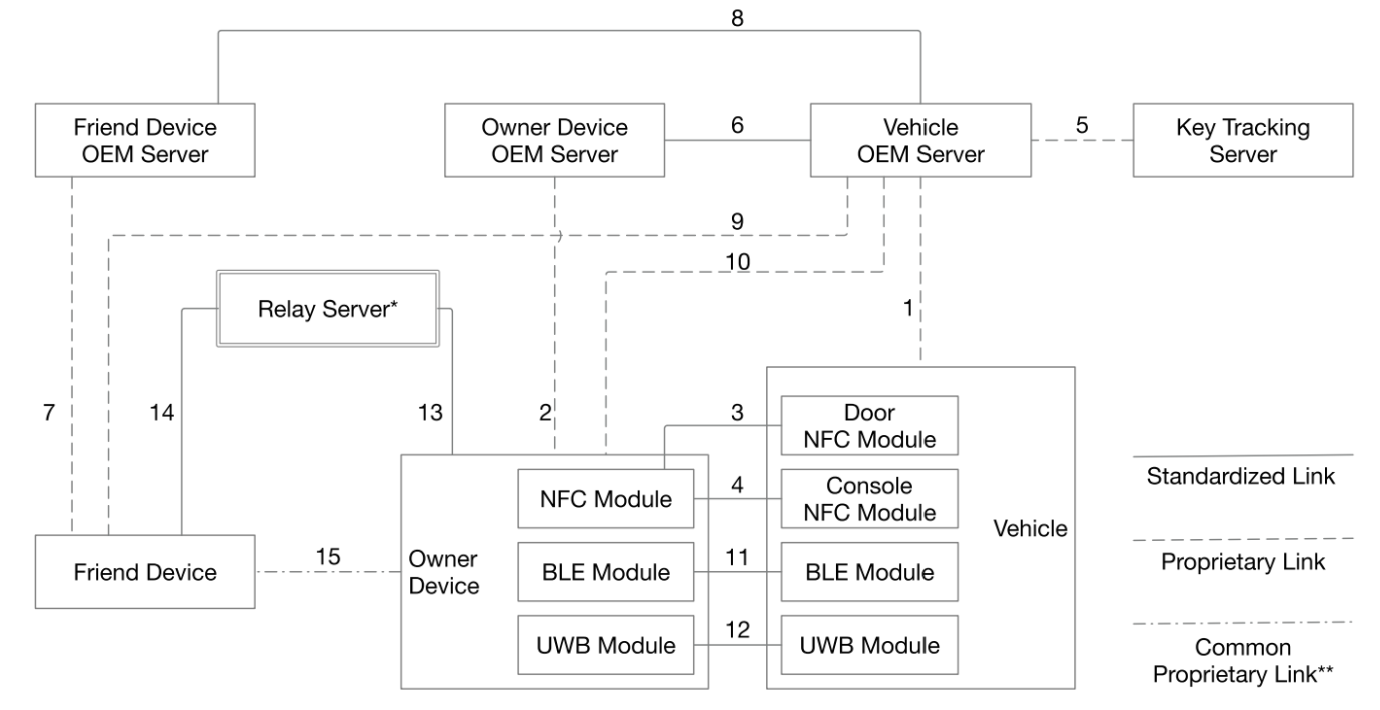
\includegraphics[width=0.8\textwidth]{image/section3/ccc_architecture.png} 
    \caption[Kiến trúc giao tiếp NFC, BLE và UWB theo chuẩn CCC 3.0]{Kiến trúc giao tiếp NFC, BLE và UWB theo chuẩn CCC 3.0 (\textbf{Nguồn:} \href{https://www.researchgate.net/publication/396275938_Mitigating_Relay_Attacks_in_Vehicle_Access_Systems_Using_BLE_and_UWB}{researchgate.net})}
    \label{fig:ccc_architecture}
\end{figure}

\subsection{Cơ chế chuyển trạng thái trong kiến trúc CCC}
Để đảm bảo luồng hoạt động chặt chẽ, chuẩn CCC định nghĩa các pha giao dịch mật mã như sau:
\begin{itemize}
    \item \textbf{Standard Transaction (Giao dịch tiêu chuẩn):} Là quá trình xác thực đầy đủ, bao gồm việc trao đổi chứng chỉ (Certificates) và khóa công khai (Public Keys) thông qua đường cong Elliptic (ECC). Pha này thường diễn ra ở lần kết nối đầu tiên hoặc khi cần thiết lập lại độ tin cậy.
    \item \textbf{Fast Transaction (Giao dịch nhanh):} Được tối ưu hóa cho các lần kết nối tiếp theo. Giao dịch này bỏ qua bước trao đổi chứng chỉ nặng nề, sử dụng lại các tham số đã được thỏa thuận trước đó để tăng tốc độ phản hồi khi người dùng bước lại gần xe, đảm bảo trải nghiệm liền mạch (Seamless experience).
\end{itemize}

Việc đề tài lấy chuẩn CCC Digital Key Release 3.0 làm kim chỉ nam thiết kế đòi hỏi hệ thống phải nắm vững và làm chủ đồng thời ba nhóm lý thuyết lõi: Công nghệ truyền thông vô tuyến, Mật mã học ứng dụng, và Kiến trúc vi điều khiển. Các nền tảng lý thuyết này sẽ được trình bày chi tiết trong các mục tiếp theo.

\section{Công nghệ truyền thông không dây}

Hệ thống Smart Car Access Control sử dụng ba công nghệ truyền thông không dây chính: NFC (Near Field Communication), BLE (Bluetooth Low Energy), và UWB (Ultra-Wideband). Mỗi công nghệ có đặc điểm riêng về phạm vi hoạt động, tốc độ truyền dữ liệu, công suất tiêu thụ và use cases phù hợp. Phần này trình bày chi tiết nguyên lý hoạt động, kiến trúc giao thức và ứng dụng của từng công nghệ.

\subsection{Near Field Communication - NFC}

\subsubsection{Giới thiệu và đặc điểm kỹ thuật} Near Field Communication (NFC) là công nghệ truyền thông không dây tầm ngắn hoạt động ở tần số \textbf{13.56 MHz} thuộc băng tần ISM (Industrial, Scientific and Medical) \cite{coskun2013professional}. NFC được phát triển dựa trên công nghệ RFID (Radio-Frequency Identification) và được chuẩn hóa bởi tổ chức ISO/IEC theo các tiêu chuẩn ISO/IEC 14443 và ISO/IEC 18092 \cite{iso14443}.

\begin{figure}[H]
    \centering
    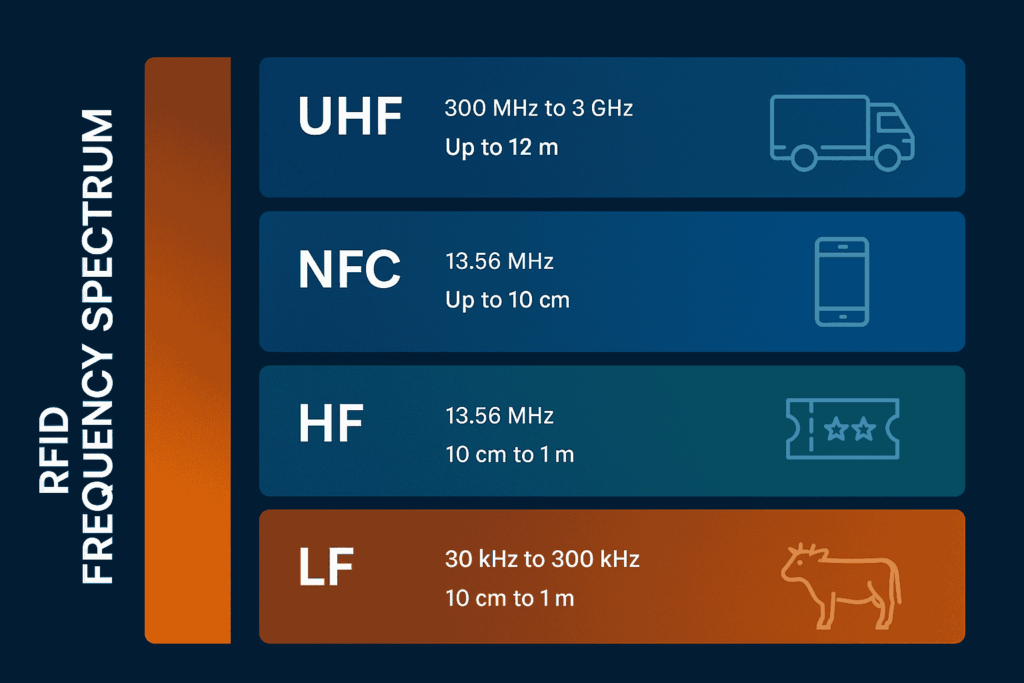
\includegraphics[width=0.8\textwidth]{image/section3/nfc.png} 
    \caption[NFC Frequency Spectrum Diagram]{NFC Frequency Spectrum Diagram (\textbf{Nguồn:} \href{https://altavantconsulting.com/fr/rfid-tag-comparison/}{Altavant})}
    \label{fig:nfc_frequency}
\end{figure}


Các đặc điểm kỹ thuật chính của NFC bao gồm:

\begin{table}[h]
\centering
\label{tab:nfc_specs}
\begin{tabular}{|l|l|}
\hline
\textbf{Thông số} & \textbf{Giá trị} \\
\hline
Tần số hoạt động & 13.56 MHz \\
Phạm vi truyền thông & < 10 cm (thông thường 4-5 cm) \\
Tốc độ truyền dữ liệu & 106, 212, 424, 848 kbps \\
Thời gian thiết lập kết nối & < 0.1 giây \\
Công suất tiêu thụ & Passive: 0 mW, Active: < 15 mA \\
Chuẩn hóa & ISO/IEC 14443, ISO/IEC 18092 \\
\hline
\end{tabular}
\caption{Thông số kỹ thuật của NFC \cite{coskun2013professional,iso14443,iso18092}}
\end{table}

Phạm vi hoạt động rất ngắn của NFC (nhỏ hơn 10 cm) là một đặc tính quan trọng giúp đảm bảo bảo mật ở mức vật lý (Physical security). Do yêu cầu thiết bị phải ở khoảng cách rất gần, kẻ tấn công gặp nhiều khó khăn trong việc nghe lén dữ liệu (Eavesdropping) hoặc thực hiện tấn công trung gian (MITM) trong quá trình giao tiếp \cite{haselsteiner2006security}.

\subsubsection{Nguyên lý hoạt động}

NFC hoạt động dựa trên nguyên lý \textbf{inductive coupling} (ghép nối cảm ứng) giữa hai cuộn dây antenna ở khoảng cách gần. Khi một thiết bị NFC (initiator/reader) phát ra từ trường RF tại tần số 13.56 MHz, từ trường này cảm ứng điện áp trong cuộn dây của thiết bị thụ động (target/tag), cung cấp năng lượng cho chip và cho phép truyền dữ liệu \cite{finkenzeller2010rfid}.

\begin{figure}[H]
    \centering
    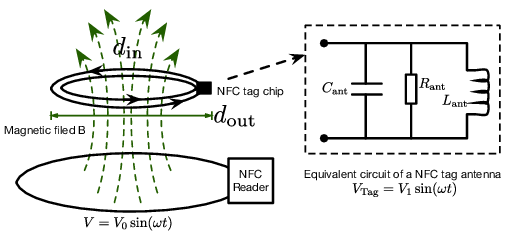
\includegraphics[width=0.8\textwidth]{image/section3/nfc2.png} 
    \caption[Sơ đồ minh họa trường từ tính giữa Reader và Tag]{Sơ đồ minh họa trường từ tính giữa Reader và Tag (\textbf{Nguồn:} \href{https://www.researchgate.net/publication/350040273_One_tag_two_codes_identifying_optical_barcodes_with_NFC}{ResearchGate})}
    \label{}
\end{figure}


Quá trình truyền dữ liệu được thực hiện thông qua cơ chế \textbf{điều chế tải} (\textit{load modulation}):

\begin{enumerate}
\item \textbf{Thiết bị đọc → Thẻ (Kênh truyền xuôi):}
Thiết bị đọc phát sóng mang tần số \textbf{13.56 MHz}, được điều chế bằng \textbf{ASK} (\textit{Amplitude Shift Keying – điều chế dịch biên độ}) với độ sâu điều chế \textbf{10\% hoặc 100\%} theo tiêu chuẩn \textbf{ISO/IEC 14443} loại A/B.

\item \textbf{Thẻ → Thiết bị đọc (kênh truyền ngược):}  
Thẻ thay đổi trở kháng của anten bằng cách bật hoặc tắt điện trở tải, tạo ra sự biến thiên điện áp trên cuộn dây của thiết bị đọc (cơ chế \textit{load modulation}). Thiết bị đọc phát hiện các thay đổi này và giải mã thành dữ liệu.
\end{enumerate}

Kỹ thuật này cho phép tag hoạt động ở chế độ passive (không cần pin) trong khi vẫn có thể truyền dữ liệu về reader \cite{coskun2013professional}.

\subsubsection{Ba chế độ hoạt động của NFC}

NFC hỗ trợ ba chế độ hoạt động chính theo chuẩn ISO/IEC 18092 \cite{iso18092}:
\par\vspace{0.5em}
\textbf{1. Reader/Writer Mode:}
\par\vspace{0.3em}
Trong chế độ này, thiết bị NFC hoạt động như một bộ đọc (Reader) để đọc và ghi dữ liệu từ các thẻ NFC thụ động (Passive NFC tags). Các ứng dụng phổ biến bao gồm:
\begin{itemize}
    \item Đọc \textbf{Smart poster} (thẻ NFC chứa địa chỉ web \textit{URL} hoặc nội dung văn bản)
    \item Đọc các thẻ theo chuẩn \textbf{NFC Forum Type~1--4}
    \item Ghi dữ liệu theo định dạng \textbf{NDEF (NFC Data Exchange Format)} lên thẻ
\end{itemize}

\begin{figure}[H]
    \centering
    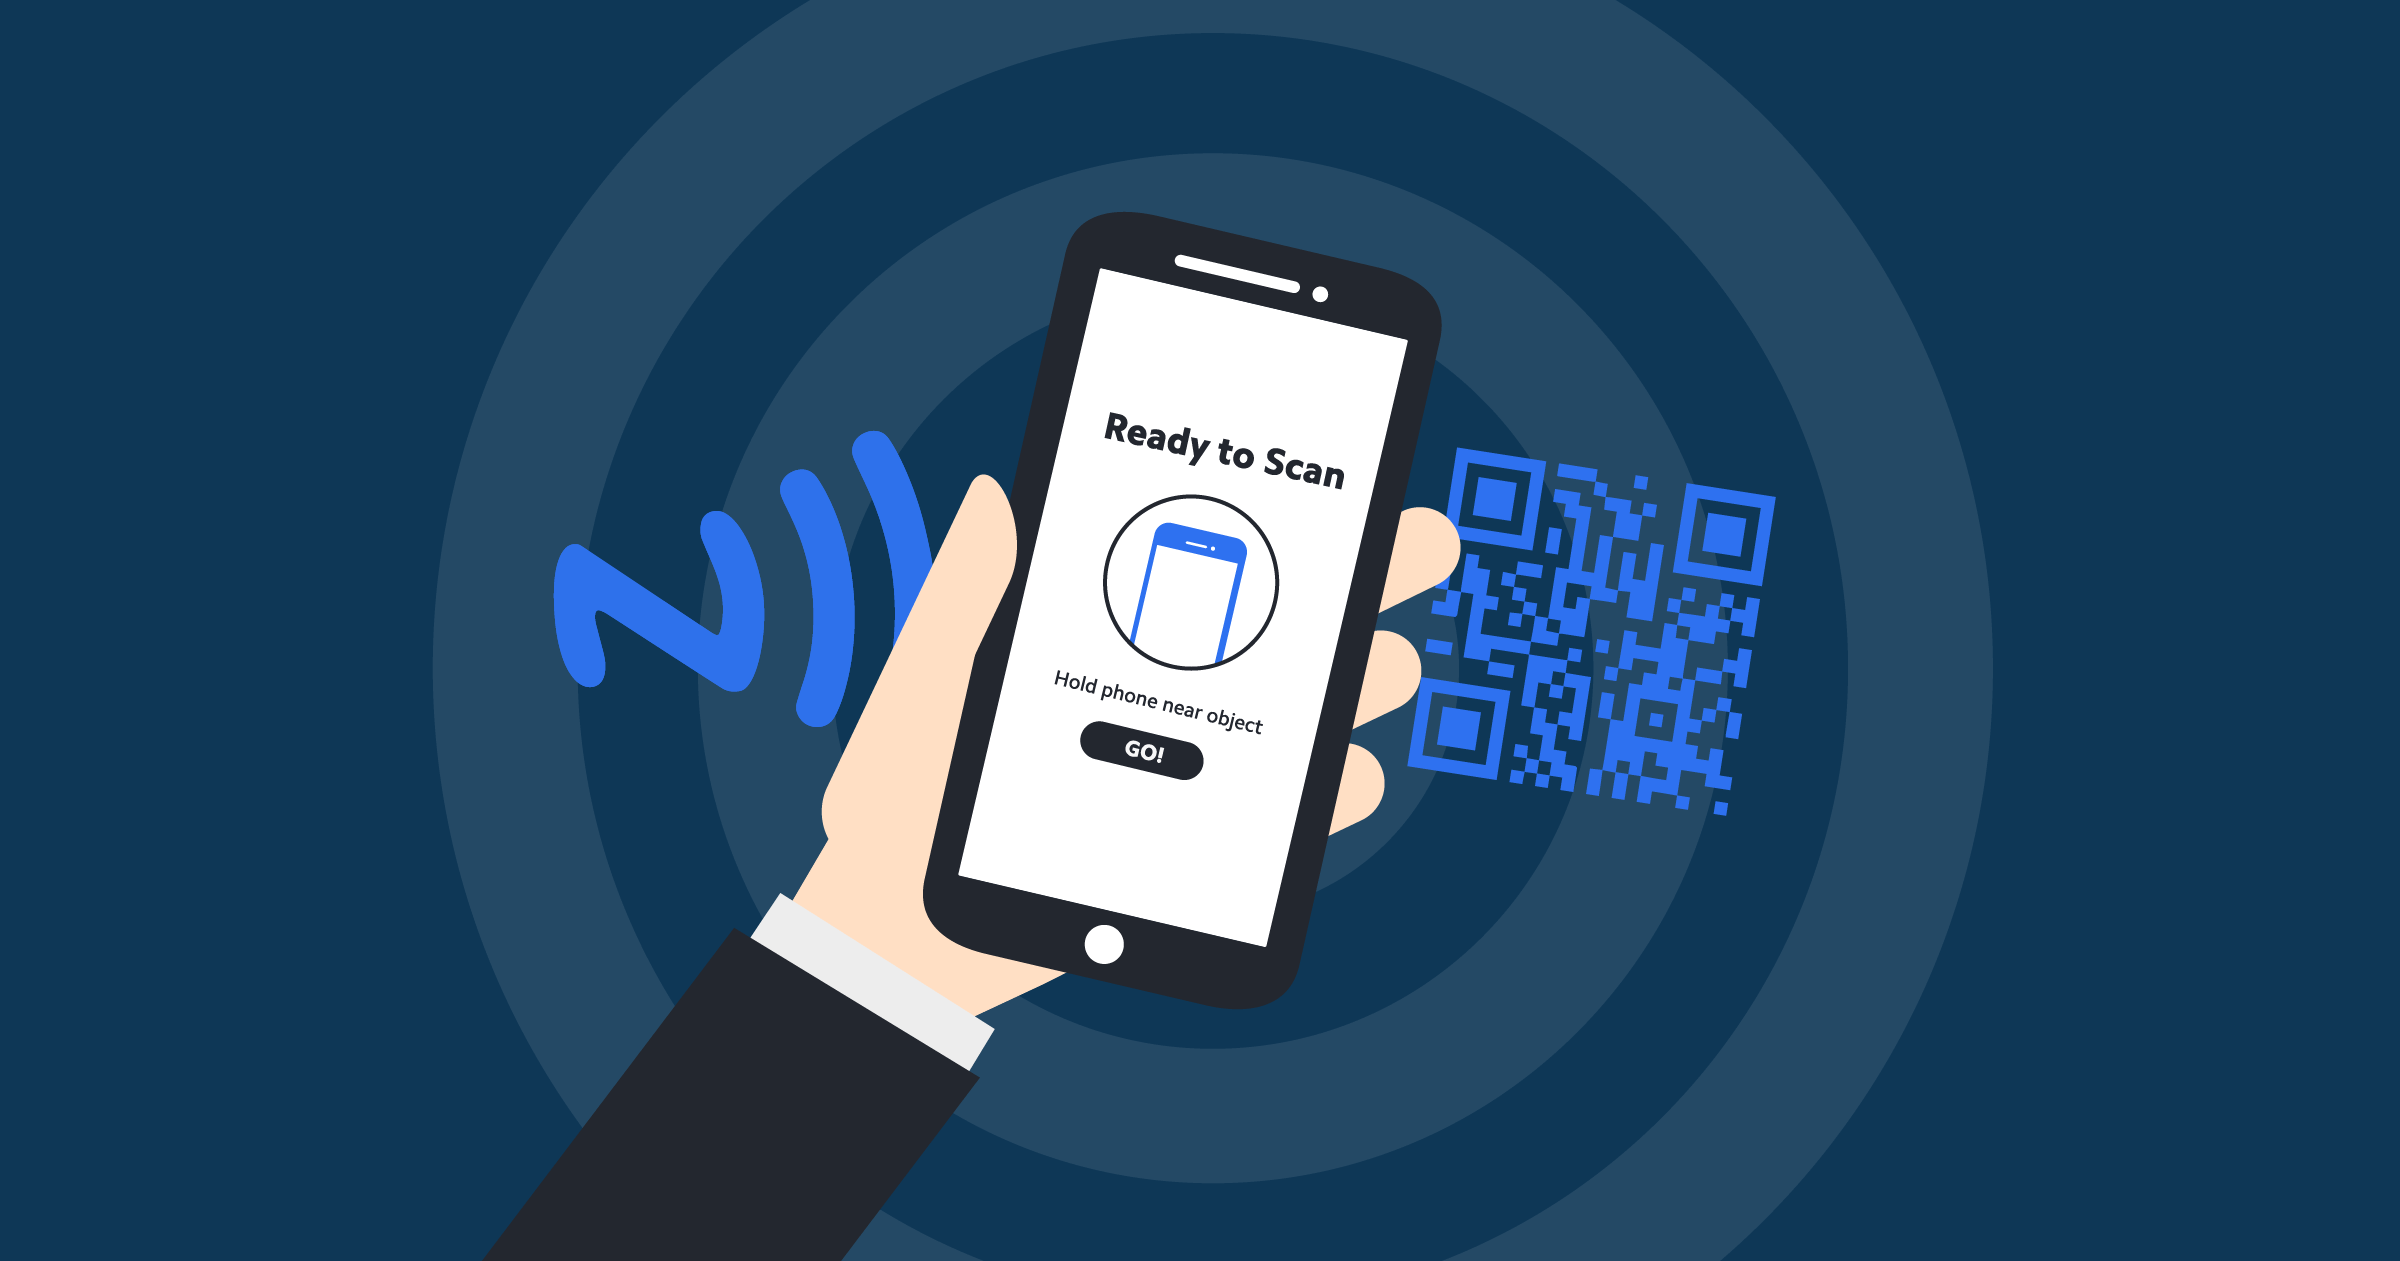
\includegraphics[width=0.8\textwidth]{image/section3/nfc3.png} 
    \caption[NFC Reader/Writer Mode]{NFC Reader/Writer Mode (\textbf{Nguồn:} \href{https://bluebite.medium.com/how-to-scan-nfc-tags-or-qr-codes-b71b8d92dd5}{Blue Bite})}
    \label{}
\end{figure}

\par\vspace{0.8em}
\textbf{2. Peer-to-Peer Mode (P2P):}

\par\vspace{0.3em}

Hai thiết bị NFC chủ động giao tiếp trực tiếp với nhau thông qua giao thức \textbf{LLCP (Logical Link Control Protocol)}. Trong quá trình trao đổi dữ liệu, hai thiết bị luân phiên phát trường sóng vô tuyến (RF field) theo cơ chế phân chia theo thời gian (Time-division multiplexing). Các ứng dụng tiêu biểu bao gồm:
\begin{itemize}
    \item \textbf{Android Beam}: truyền tệp và chia sẻ danh bạ
    \item Ghép nối \textbf{Bluetooth} thông qua cơ chế \textbf{NFC handover}
    \item Chia sẻ thông tin xác thực mạng \textbf{Wi-Fi}
\end{itemize}

\par\vspace{0.8em}
\textbf{3. Card Emulation Mode:}

\par\vspace{0.3em}
Thiết bị NFC (thường là điện thoại thông minh) giả lập một thẻ NFC hoặc thẻ thông minh (Smart card), cho phép tương tác trực tiếp với các thiết bị đầu cuối đã được triển khai sẵn trong hạ tầng. Hiện nay tồn tại hai hướng triển khai chính \cite{madlmayr2008nfc}:

\begin{itemize}
    \item \textbf{Dựa trên Secure Element (SE):} 
    Sử dụng phần cứng bảo mật chuyên dụng (embedded SE, thẻ SIM hoặc thẻ microSD) để lưu trữ dữ liệu nhạy cảm và thực hiện các phép toán mật mã. Cách tiếp cận này cung cấp mức độ bảo mật cao nhờ khả năng chống can thiệp vật lý, tuy nhiên quy trình cấp phát và quản lý khóa (Provisioning) phức tạp.

    \item \textbf{Host Card Emulation (HCE):} 
    Việc giả lập thẻ được thực hiện trực tiếp bởi bộ xử lý ứng dụng (Application processor – CPU chính của điện thoại thông minh) mà không cần sử dụng Secure Element. Nền tảng Android (từ phiên bản 4.4 trở lên) hỗ trợ HCE \cite{android_security}, và iOS (từ phiên bản 13 trở lên) cũng hỗ trợ HCE. Trong phạm vi đề tài này, HCE được lựa chọn để triển khai giai đoạn cấp phát khóa (Provisioning).
\end{itemize}

\begin{figure}[H]
    \centering
    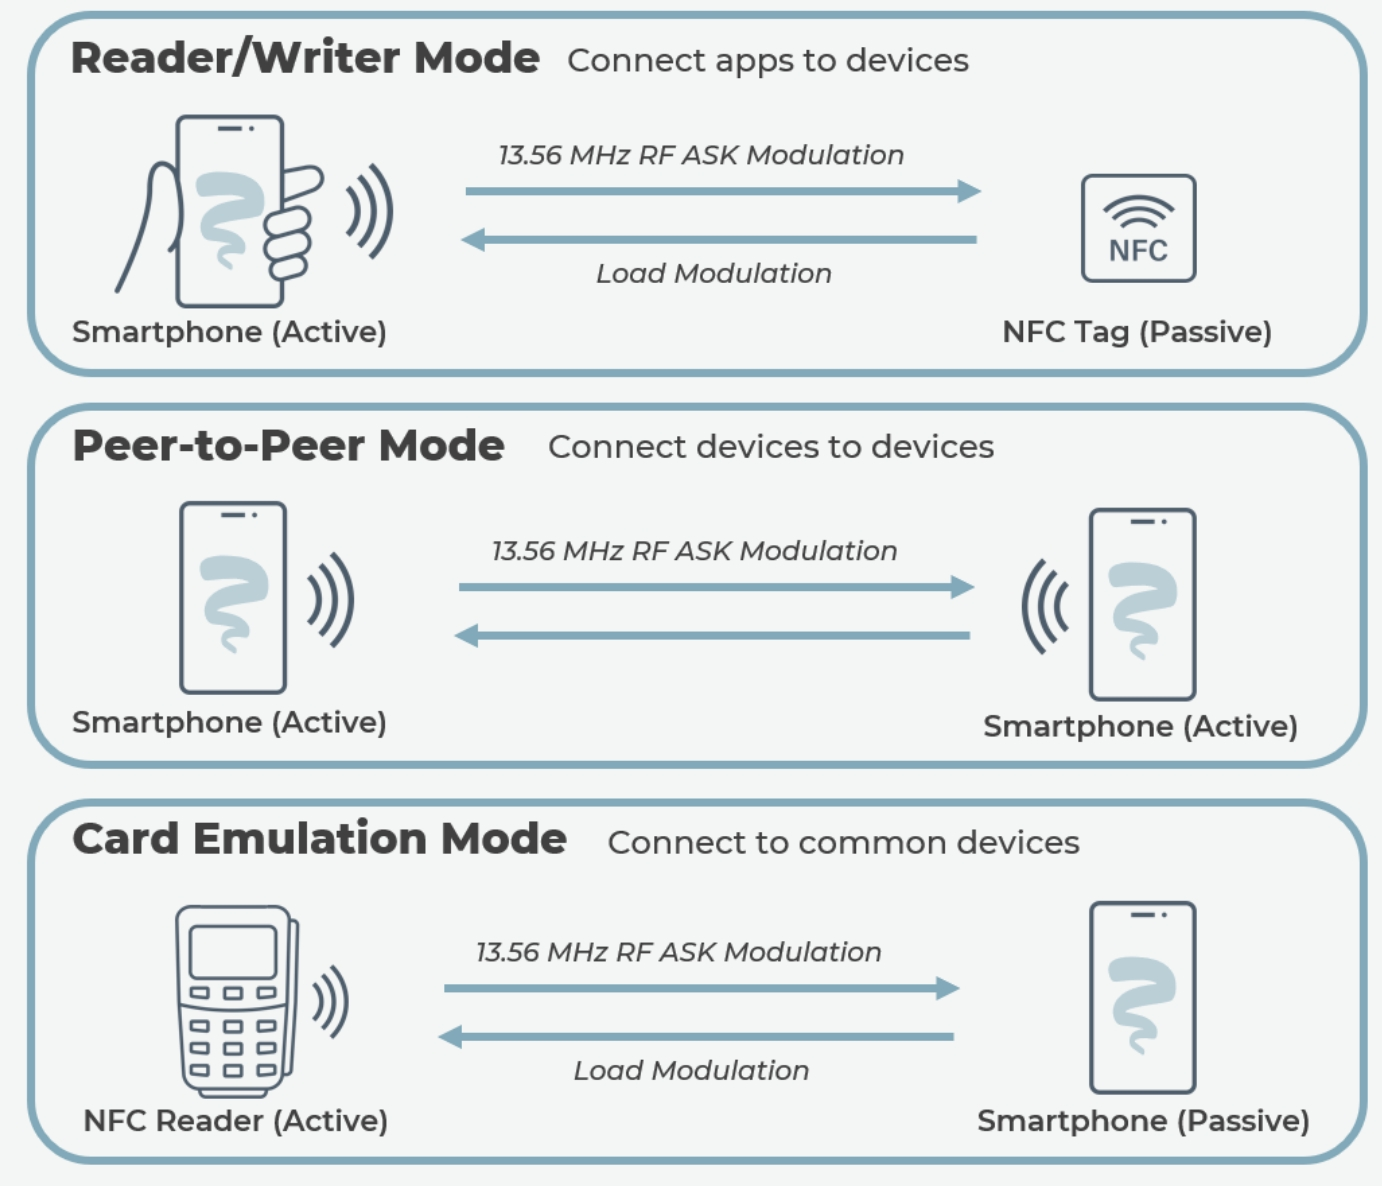
\includegraphics[width=0.8\textwidth]{image/section3/nfc4.jpeg} 
    \caption[So sánh 3 chế độ của NFC]{So sánh 3 chế độ của NFC (\textbf{Nguồn:} \href{https://www.cardinalpeak.com/blog/counterfeit-protection-exploring-the-role-of-nfc-in-the-iot}{Cardinal Peak})}
    \label{}
\end{figure}


\subsubsection{Giao thức APDU}

Trong chế độ giả lập thẻ (card emulation mode), giao tiếp giữa đầu đọc 
(reader) và thẻ (card) sử dụng \textbf{giao thức APDU (Application Protocol 
Data Unit)} theo chuẩn ISO/IEC 7816-4 \cite{iso7816}. APDU là đơn vị dữ 
liệu ở tầng ứng dụng cho phép truyền các lệnh và phản hồi  giữa hai thiết bị.

\textbf{Command APDU (từ reader → card):}

\begin{table}[h]
\centering
\label{tab:command_apdu}
\begin{tabular}{|l|l|l|}
\hline
\textbf{Field} & \textbf{Size} & \textbf{Mô tả} \\
\hline
CLA & 1 byte & Class byte (instruction class) \\
INS & 1 byte & Instruction byte (command) \\
P1 & 1 byte & Parameter 1 \\
P2 & 1 byte & Parameter 2 \\
Lc & 1 byte & Length of command data \\
Data & Variable & Command data (if Lc > 0) \\
Le & 1 byte & Expected response length \\
\hline
\end{tabular}
\caption{Cấu trúc Command APDU}
\end{table}

\textbf{Response APDU (từ card → reader):}

\begin{table}[h]
\centering
\label{tab:response_apdu}
\begin{tabular}{|l|l|l|}
\hline
\textbf{Field} & \textbf{Size} & \textbf{Mô tả} \\
\hline
Data & Variable & Response data \\
SW1 & 1 byte & Status word 1 \\
SW2 & 1 byte & Status word 2 \\
\hline
\end{tabular}
\caption{Cấu trúc Response APDU}
\end{table}

Status words (SW1 SW2) chỉ định kết quả xử lý command:
\begin{itemize}
    \item \texttt{90 00}: Success (Normal processing)
    \item \texttt{6A 82}: File not found
    \item \texttt{6A 86}: Incorrect parameters P1-P2
    \item \texttt{67 00}: Wrong length (Lc hoặc Le)
\end{itemize}

\textbf{Ví dụ: SELECT AID Command}

Để chọn một application trên NFC card, reader gửi SELECT command với Application Identifier (AID):

\noindent\begin{minipage}{\linewidth}
\begin{lstlisting}[language=C++, caption={NFC SELECT AID Command}]
Command:  00 A4 04 00 06 F0 01 02 03 04 05 00
          |  |  |  |  |  |              |  |
          |  |  |  |  |  |              |  Le (expected length)
          |  |  |  |  |  Data (AID: F00102030405)
          |  |  |  |  Lc (length = 6 bytes)
          |  |  P1 P2 (04 00 = select by name)
          |  INS (A4 = SELECT)
          CLA (00 = inter-industry class)

Response: 90 00
          |  |
          |  SW2
          SW1 (success)
\end{lstlisting}
\end{minipage}


\subsubsection{Bảo mật NFC}

NFC cung cấp một số đặc điểm bảo mật tự nhiên nhờ phạm vi hoạt động ngắn \cite{haselsteiner2006security}:
\par\vspace{0.5em}
\textbf{Ưu điểm:}
\begin{itemize}
    \item \textbf{Physical proximity:} Yêu cầu khoảng cách < 10 cm giảm thiểu bị nghe lén thông tin cá nhân
    \item \textbf{No pairing required:} Không cần setup phức tạp như Bluetooth
    \item \textbf{Fast connection:} Transaction time < 0.1s, khó can thiệp
\end{itemize}

\textbf{Các mối đe dọa và biện pháp:}
\begin{itemize}
    \item \textbf{Nghe lén (Eavesdropping):} 
    Kẻ tấn công có thể đặt ăng-ten ở khoảng cách gần để thu thập tín hiệu vô tuyến (RF signal) trong quá trình truyền dữ liệu. 

    
    \textit{Biện pháp:} Áp dụng cơ chế mã hóa ở tầng ứng dụng (Application layer), cụ thể trong đề tài này là sử dụng chữ ký số ECDSA để bảo vệ nội dung trao đổi.

    \item \textbf{Sửa đổi dữ liệu (Data Modification):} 
    Các tấn công chủ động (Active attack) có thể can thiệp và thay đổi dữ liệu trong quá trình truyền.

    
    \textit{Biện pháp:} Sử dụng chữ ký số (Digital signature) kết hợp với cơ chế kiểm tra toàn vẹn dữ liệu (Integrity checking).

    \item \textbf{Tấn công chuyển tiếp (Relay Attack):} 
    Kẻ tấn công sử dụng hai thiết bị trung gian để chuyển tiếp (Relay) quá trình giao tiếp giữa bộ đọc (Reader) và thẻ (Card) ở khoảng cách xa.

    
    \textit{Biện pháp:} Triển khai giao thức hỏi–đáp (challenge–response protocol) có gắn dấu thời gian (Timestamp); trong phạm vi đề tài, cơ chế này được hiện thực thông qua việc xác thực chữ ký ECDSA.
\end{itemize}


Theo nghiên cứu của Haselsteiner và Breitfuß (2006), công nghệ NFC có thể cung cấp mức độ bảo mật tương đương với thẻ thông minh tiếp xúc trực tiếp (Contact smart cards) khi được kết hợp với các giao thức mật mã phù hợp (Cryptographic protocols) \cite{haselsteiner2006security}.


\subsection{Bluetooth Low Energy - BLE}

\subsubsection{Giới thiệu và đặc điểm kỹ thuật}

Bluetooth Low Energy (BLE), còn được gọi là Bluetooth Smart, là phiên bản tiết kiệm năng lượng của Bluetooth Classic, được giới thiệu trong \textbf{Bluetooth 4.0 specification} năm 2010 bởi Bluetooth SIG (Special Interest Group) \cite{bluetooth40}. BLE được thiết kế đặc biệt cho các ứng dụng IoT yêu cầu battery life lâu (từ vài tháng đến vài năm) với cost thấp \cite{gomez2012overview,heydon2013bluetooth,townsend2014getting}.

\begin{figure}[H]
    \centering
    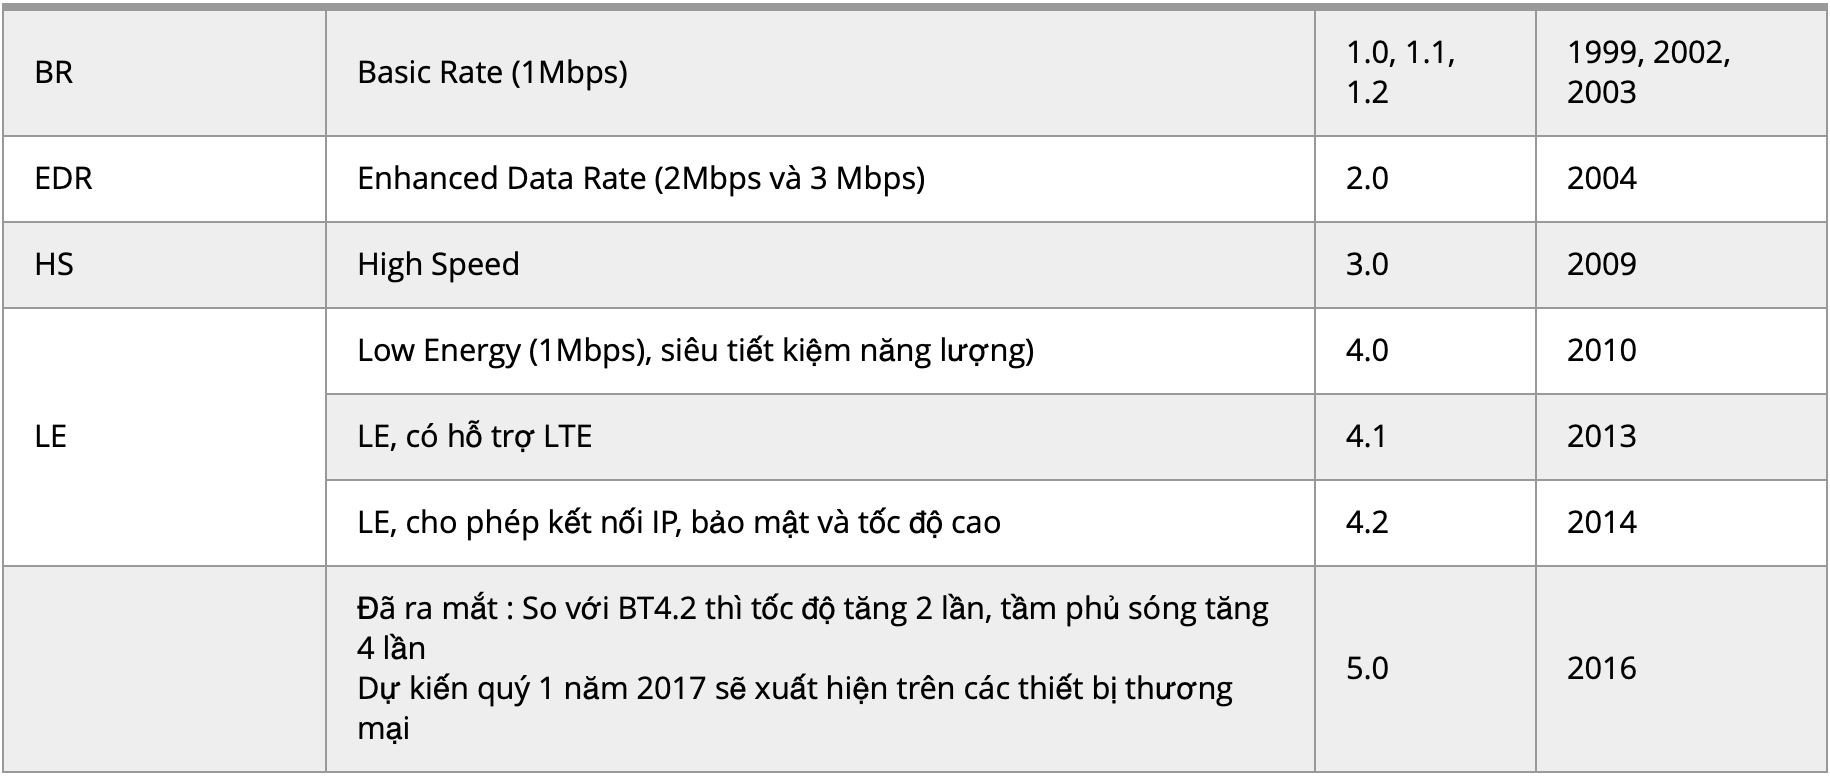
\includegraphics[width=0.8\textwidth]{image/section3/bluetooth2.png} 
    \caption[Sự phát triển của công nghệ Bluetooth qua các thời kỳ]{Sự phát triển của công nghệ Bluetooth qua các thời kỳ (\textbf{Nguồn:} \href{https://vngiotlab.github.io/vbluno/vi/mydoc_ble_vi.html}{VBLUno51 board})}
    \label{}
\end{figure}

\begin{table}[h]
\centering
\label{tab:ble_vs_classic}
\begin{tabular}{|l|l|l|}
\hline
\textbf{Đặc điểm} & \textbf{BLE} & \textbf{Bluetooth Classic} \\
\hline
Băng tần hoạt động & 2.4 GHz ISM & 2.4 GHz ISM \\
Số kênh truyền & 40 kênh (khoảng cách 2 MHz) & 79 kênh (khoảng cách 1 MHz) \\
Phạm vi hoạt động & 10--50 m (Class 2) & 10--100 m \\
Tốc độ dữ liệu & 1 Mbps (Bluetooth 4.x) & 1--3 Mbps \\
                & 2 Mbps (Bluetooth 5.x) &  \\
Độ trễ (Latency) & 6 ms & 100 ms \\
Dòng tiêu thụ cực đại & 15 mA & 30 mA \\
Công suất tiêu thụ & 0.01--0.5 W & 1 W \\
Ứng dụng điển hình & Cảm biến, thiết bị đeo & Âm thanh, truyền tệp \\
\hline
\end{tabular}
\caption{So sánh Bluetooth Low Energy (BLE) và Bluetooth Classic \cite{bluetooth40,ble_core,gomez2012overview}}
\end{table}


BLE sử dụng \textbf{40 kênh vô tuyến (RF channels)} trong băng tần \textbf{2.4 GHz} (từ 2.400 đến 2.4835 GHz) \cite{gomez2012overview}, bao gồm:

\begin{itemize}
    \item \textbf{3 kênh quảng bá (Advertising channels):} Các kênh 37, 38 và 39 (tương ứng với các tần số 2.402 GHz, 2.426 GHz và 2.480 GHz) được lựa chọn nhằm giảm thiểu nhiễu từ các kênh Wi-Fi phổ biến (kênh 1, 6 và 11).
    
    \item \textbf{37 kênh dữ liệu (Data channels):} Các kênh từ 0 đến 36 được sử dụng cho quá trình truyền dữ liệu sau khi các thiết bị đã thiết lập kết nối.
\end{itemize}


\begin{figure}[H]
    \centering
    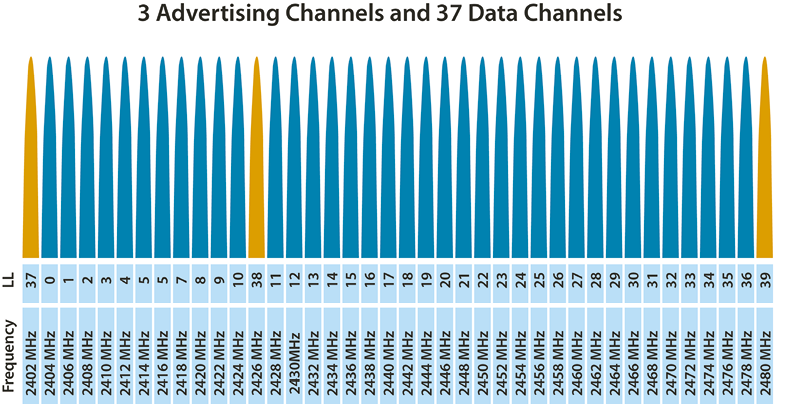
\includegraphics[width=0.8\textwidth]{image/section3/blemap.png} 
    \caption[Biểu đồ 40 kênh BLE]{Biểu đồ 40 kênh BLE (\textbf{Nguồn:} \href{https://www.researchgate.net/figure/Bluetooth-low-energy-channels-and-frequencies_fig7_310500994}{ResearchGate})}
    \label{fig:ble_channels}
\end{figure}


\subsubsection{Kiến trúc giao thức BLE}

Giao thức BLE được tổ chức thành nhiều tầng theo mô hình OSI 
\cite{townsend2014getting,bluetooth40}:

\begin{enumerate}
    \item \textbf{Tầng vật lý (Physical Layer - PHY):} 
    
    Xử lý bộ thu phát RF, điều chế tín hiệu GFSK (Gaussian Frequency Shift 
    Keying), và nhảy tần. Phiên bản BLE 5.0 bổ sung hai chế độ PHY mới: 
    2 Mbps cho tốc độ cao và 125/500 kbps cho khoảng cách xa 
    \cite{ble_core}.
    
    \item \textbf{Tầng liên kết (Link Layer - LL):}
    
    Quản lý quảng bá (Advertising), quét tìm (Scanning), thiết lập kết nối, 
    và truyền gói dữ liệu. Tầng này định nghĩa năm trạng thái thiết bị: 
    Standby, Advertising, Scanning, Initiating, và Connection 
    \cite{gomez2012overview}.
    
    \item \textbf{Giao diện điều khiển máy chủ (Host Controller Interface - HCI):}
    
    Cung cấp giao diện chuẩn hóa giữa máy chủ (application processor) và 
    bộ điều khiển (BLE chip), thường sử dụng UART, USB, hoặc SDIO 
    \cite{bluetooth40}.
    
    \item \textbf{Logical Link Control and Adaptation Protocol - L2CAP:}
    
    Thực hiện phân mảnh và tái lắp ráp gói tin, ghép kênh các giao thức, 
    và đảm bảo chất lượng dịch vụ. BLE sử dụng phiên bản L2CAP đơn giản 
    hóa so với Bluetooth Classic \cite{heydon2013bluetooth}.
    
    \item \textbf{Attribute Protocol - ATT:}
    
    Định nghĩa cách thức client truy cập các thuộc tính trên server thông 
    qua các thao tác Read, Write, Notify và Indicate. Mỗi thuộc tính có 
    handle (định danh 16-bit), type (UUID), và giá trị \cite{bluetooth40}.
    
    \item \textbf{Generic Attribute Profile - GATT:}
    
    Xây dựng trên ATT, định nghĩa cách tổ chức các thuộc tính thành dịch vụ 
    (Services) và đặc tính (Characteristics). GATT là tầng mà các nhà phát 
    triển thường tương tác trực tiếp \cite{townsend2014getting}.
    
    \item \textbf{Generic Access Profile - GAP:}
    
    Quản lý vai trò thiết bị (Central/Peripheral), quảng bá, khám phá 
    (Discovery), và các thủ tục kết nối \cite{heydon2013bluetooth}.
\end{enumerate}


\begin{figure}[H]
    \centering
    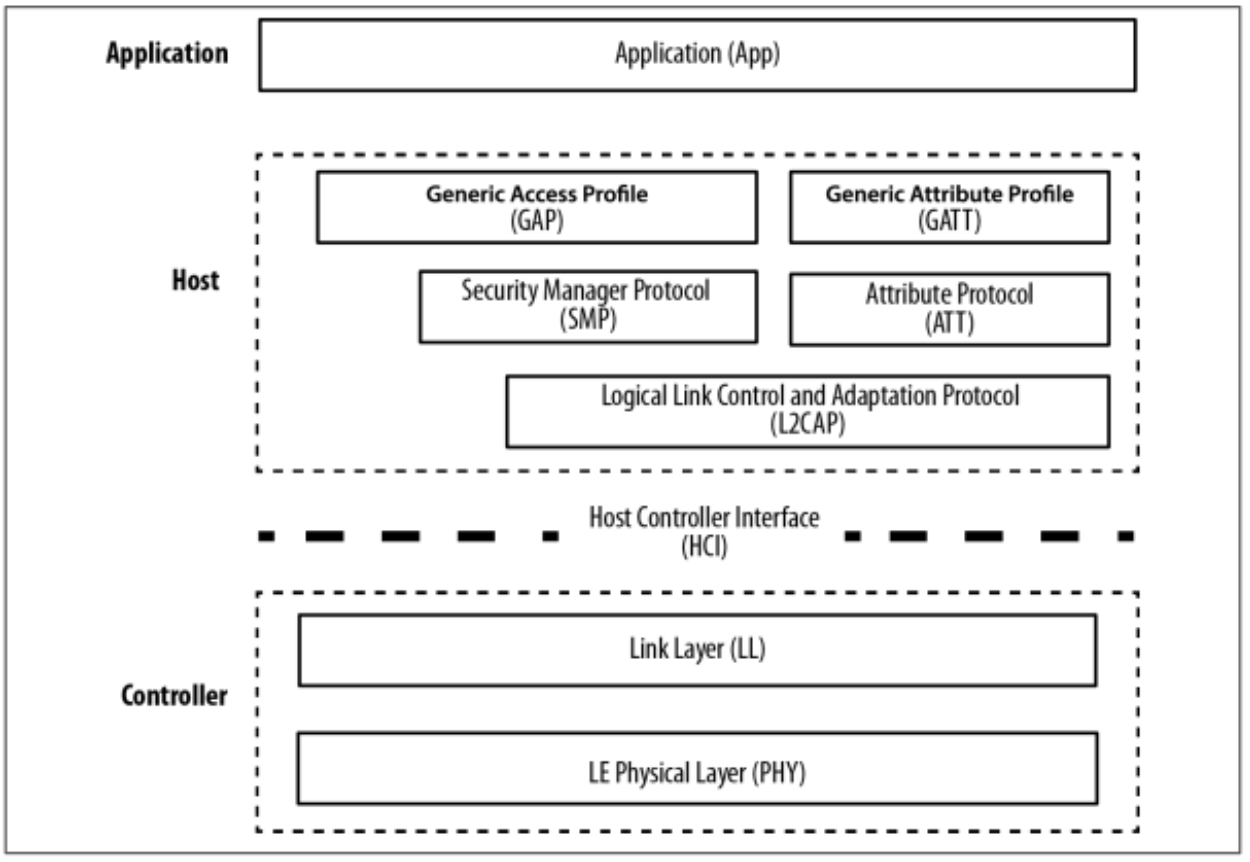
\includegraphics[width=0.8\textwidth]{image/section3/blue5.png} 
    \caption[Sơ đồ Layered Architecture của BLE]{Sơ đồ Layered Architecture của BLE (\textbf{Nguồn:} \href{https://www.researchgate.net/publication/379552583_Application_of_bluetooth_mesh_network_in_multi-device_system_management}{Researchgate})}
    \label{}
\end{figure}
\subsubsection{GATT (Generic Attribute Profile)}

GATT (Generic Attribute Profile) định nghĩa cấu trúc dữ liệu phân cấp
(Hierarchical data structure) cho các dịch vụ BLE \cite{heydon2013bluetooth}:

\noindent\begin{minipage}{\linewidth}
\begin{lstlisting}[language=C++, caption={Định nghĩa cấu trúc dữ liệu phân cấp}]
    Profile
     |
     +-- Service (UUID: 16-bit or 128-bit)
     |    |
     |    +-- Characteristic 1
     |    |    |
     |    |    +-- Value (data)
     |    |    +-- Properties (Read / Write / Notify / Indicate)
     |    |    +-- Descriptors (metadata)
     |    |         |
     |    |         +-- CCCD (Client Characteristic Configuration Descriptor)
     |    |
     |    +-- Characteristic 2
     |
     +-- Characteristic 3
\end{lstlisting}
\end{minipage}



\textbf{UUID (Universally Unique Identifier – Định danh duy nhất toàn cục):}
\begin{itemize}
    \item \textbf{UUID 16-bit:}  
    Được Bluetooth SIG quy định sẵn (Reserved) cho các dịch vụ chuẩn
    (ví dụ: Heart Rate Service = 0x180D).  
    Base UUID tương ứng:
    \texttt{0000xxxx-0000-1000-8000-00805F9B34FB}
    
    \item \textbf{UUID 128-bit:}  
    Được định nghĩa tùy chỉnh cho các dịch vụ hoặc Characteristic riêng
    do nhà phát triển thiết kế.  
    Ví dụ:
    \texttt{0000aaaa-1234-5678-9abc-def012345678}
\end{itemize}


\textbf{Thuộc tính của Characteristic (Characteristic Properties):}
\begin{table}[htbp]
\centering
\label{tab:gatt_properties}
\begin{tabular}{|l|p{10cm}|}
\hline
\textbf{Thuộc tính} & \textbf{Mô tả} \\
\hline
Read & Thiết bị Client đọc giá trị (value) thông qua bản tin ATT Read Request \\
Write & Thiết bị Client ghi giá trị và nhận phản hồi xác nhận từ server (ATT Write Request) \\
Write Without Response & Thiết bị Client ghi giá trị mà không cần chờ phản hồi xác nhận (ATT Write Command) \\
Notify & Thiết bị Server chủ động gửi dữ liệu đến client mà không yêu cầu xác nhận \\
Indicate & Thiết bị Server gửi dữ liệu đến client và yêu cầu xác nhận đã nhận (ATT Handle Value Confirmation) \\
\hline
\end{tabular}
\caption{Các thuộc tính của GATT Characteristic}
\end{table}


\textbf{Ví dụ: Heart Rate Service}

\noindent\begin{minipage}{\linewidth}
\begin{lstlisting}[language=C++, caption={Heart Rate Service}]
      Service: Heart Rate (0x180D)
       |
       +-- Characteristic: Heart Rate Measurement (0x2A37)
       |    |
       |    +-- Value: [0x16, 0x4E] -> 78 bpm
       |    +-- Properties: Notify
       |    +-- Descriptor: CCCD (0x2902)
       |         |
       |         +-- Value: [0x01, 0x00] -> Notifications enabled
       |
       +-- Characteristic: Body Sensor Location (0x2A38)
             |
             +-- Value: [0x01] -> Wrist
             +-- Properties: Read
\end{lstlisting}
\end{minipage}


\begin{figure}[H]
    \centering
    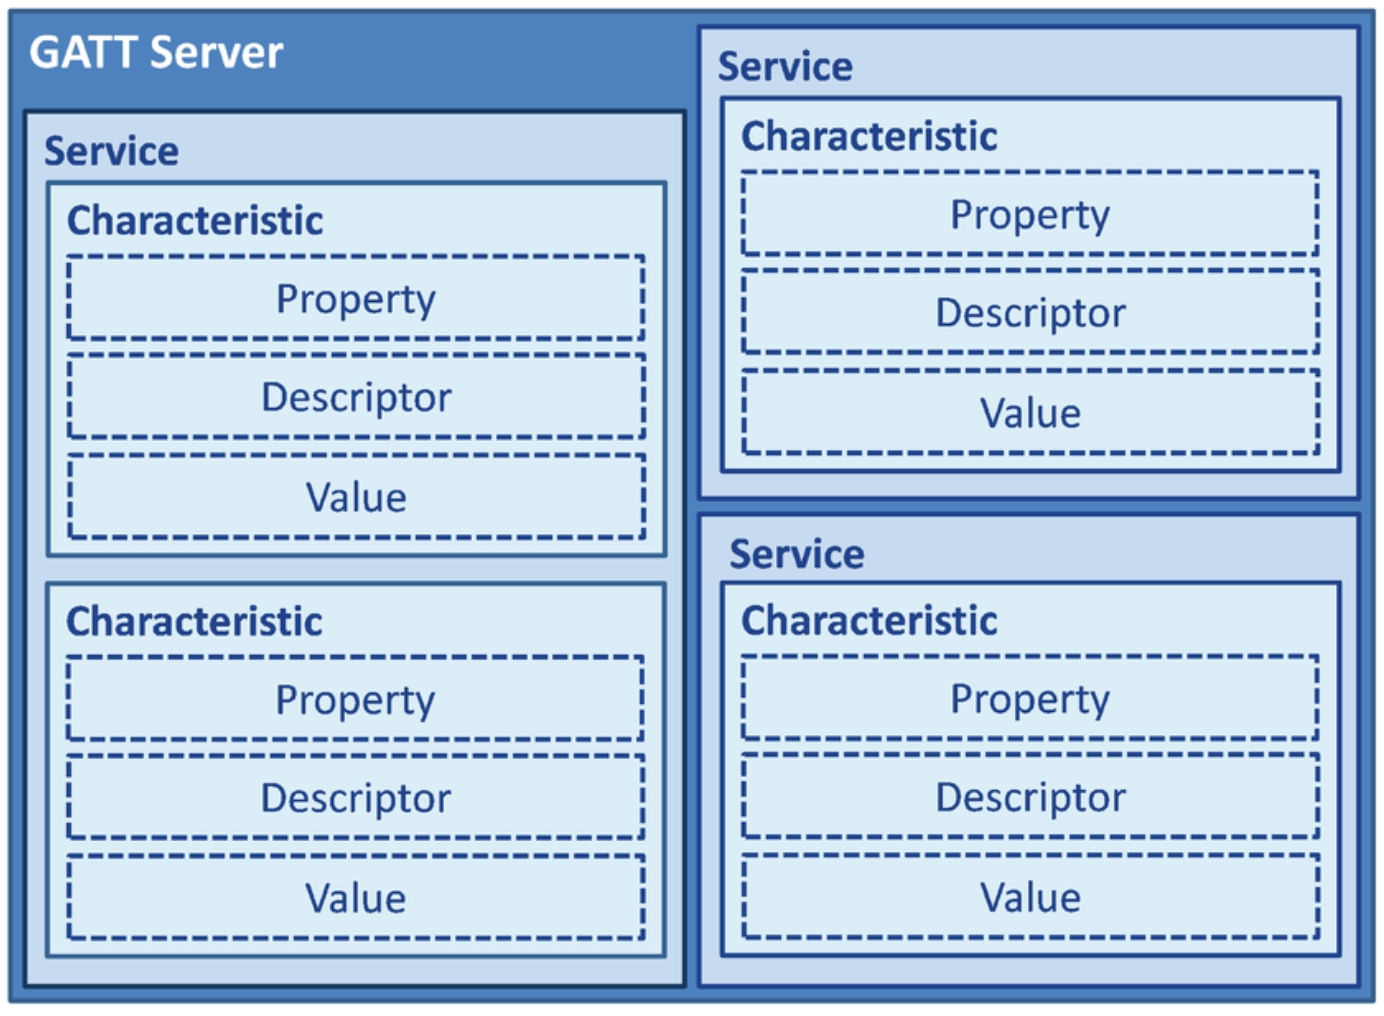
\includegraphics[width=0.8\textwidth]{image/section3/gatt.jpeg} 
    \caption[Diagram GATT Hierarchy]{Diagram GATT Hierarchy (\textbf{Nguồn:} \href{https://www.mdpi.com/1424-8220/17/12/2898}{MDPI})}
    \label{}
\end{figure}

\begin{itemize}
    \item \textbf{Handshake Write:} Smartphone gửi \emph{Ephemeral public key} kèm theo \emph{chữ ký số (Signature)} để khởi tạo phiên xác thực.
    
    \item \textbf{Handshake Read:} Smartphone đọc \emph{Ephemeral public key} do ECU sinh ra để hoàn tất quá trình trao đổi khóa tạm thời.

    \item \textbf{Status:} ECU sử dụng cơ chế \emph{Notify} để thông báo trạng  thái xác thực, bao gồm \texttt{AUTH\_SUCCESS} hoặc \texttt{AUTH\_FAILED}.

    \item \textbf{Challenge Read:} Smartphone nhận \emph{Challenge} do ECU tạo ra nhằm chống các hình thức tấn công giả mạo hoặc Relay attack.

    \item \textbf{Challenge Write:} Smartphone gửi lại \emph{chữ ký số của Challenge} để ECU kiểm tra và xác thực danh tính.
\end{itemize}

\subsubsection{Connection và Data Transfer Flow}

Quá trình thiết lập kết nối và truyền dữ liệu trong BLE bao gồm các bước chính sau đây \cite{townsend2014getting}:

\medskip
\par\vspace{0.5em}
\textbf{1. Advertising:}
\par\vspace{0.3em}
Ở giai đoạn này, thiết bị ngoại vi (Peripheral – trong đề tài là ESP32) định kỳ phát các Advertising packet trên 3 kênh quảng bá (Advertising channels).
Chu kỳ phát (Advertising interval) có thể cấu hình trong khoảng từ 20 ms đến 10.24 s \cite{bluetooth40,ble_core}.

Nội dung của Advertising packet bao gồm:
\begin{itemize}
\item Địa chỉ thiết bị (Sevice address), có thể là public address hoặc Random address
\item Tên thiết bị (Device name)
\item Danh sách các Service UUID mà thiết bị hỗ trợ
\item Mức công suất phát (TX power level)
\item Các cờ trạng thái (Flags), chẳng hạn như khả năng khám phá hoặc kết nối
\end{itemize}

\medskip
\par\vspace{0.5em}
\textbf{2. Scanning:}
\par\vspace{0.3em}
Thiết bị trung tâm (Central – smartphone) thực hiện lắng nghe các Advertising packet trên 3 Advertising channels để phát hiện thiết bị BLE ở gần.

BLE hỗ trợ hai chế độ quét (Scan mode):
\begin{itemize}
\item \textbf{Passive scanning:} Thiết bị trung tâm chỉ lắng nghe các Advertising packet mà không gửi phản hồi.

\item \textbf{Active scanning:} Sau khi nhận Advertising packet, thiết bị trung tâm gửi gói \texttt{SCAN\_REQ} để yêu cầu thêm thông tin, và Peripheral sẽ phản hồi bằng gói \texttt{SCAN\_RSP}.


\end{itemize}

\begin{figure}[H]
    \centering
    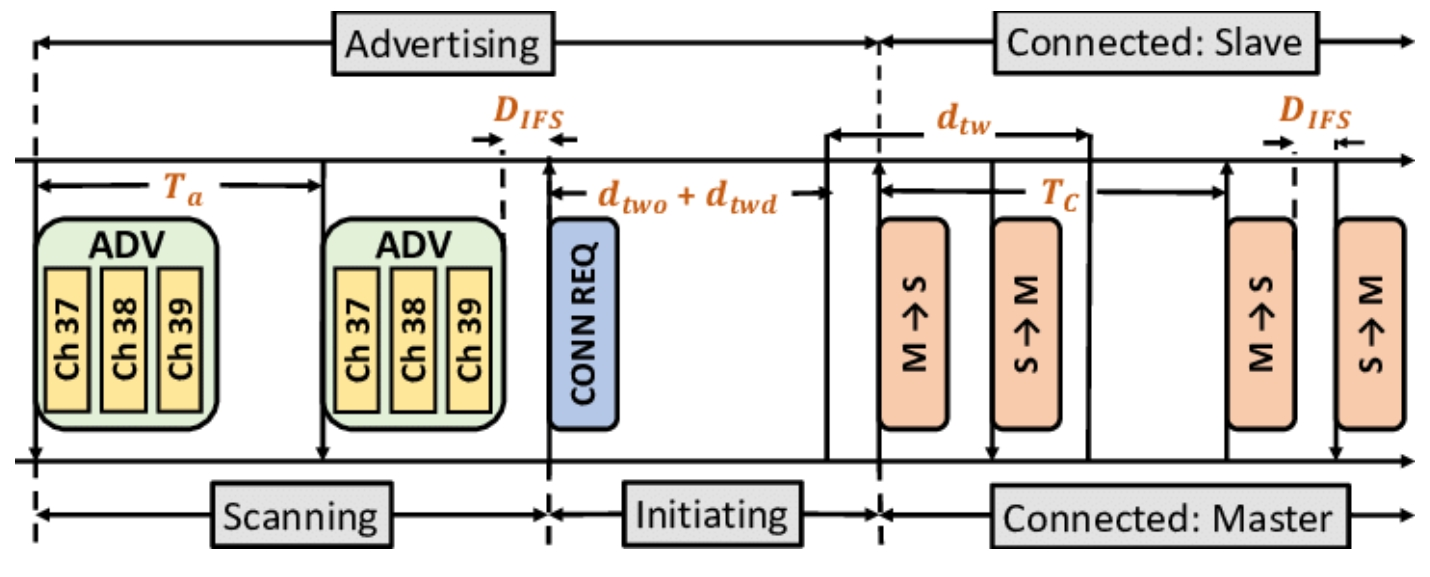
\includegraphics[width=0.8\textwidth]{image/section3/ble_flow.jpeg} 
    \caption[BLE Connection Flow]{BLE Connection Flow (\textbf{Nguồn:} \href{https://www.researchgate.net/publication/334783317_A_Robust_Algorithm_for_Sniffing_BLE_Long-Lived_Connections_in_Real-time}{ResearchGate})}
    \label{}
\end{figure}

\subsubsection{Bảo mật BLE}

BLE cung cấp nhiều cơ chế bảo mật ở tầng liên kết (Link layer) nhằm đảm bảo tính bí mật và toàn vẹn của dữ liệu \cite{bluetooth40}.

\medskip
\par\vspace{0.5em}
\textbf{1. Các phương thức ghép cặp (Pairing Methods):}
\par\vspace{0.3em}
BLE hỗ trợ nhiều phương thức ghép cặp với mức độ bảo mật khác nhau:
\begin{itemize}
\item \textbf{Just Works:}
Không cung cấp cơ chế bảo vệ chống tấn công trung gian (MITM – Man-In-The-Middle), chỉ hỗ trợ mã hóa dữ liệu sau khi ghép cặp. Phương thức này dễ bị nghe lén thụ động (Passive eavesdropping).

\item \textbf{Passkey Entry:}  
Người dùng nhập mã PIN gồm 6 chữ số để xác thực. Phương thức này có khả năng chống MITM, tuy nhiên mức độ an toàn phụ thuộc vào Entropy của mã PIN.

\item \textbf{Numeric Comparison:}  
Người dùng xác nhận hai thiết bị hiển thị cùng một mã số gồm 6 chữ số. Phương thức này cung cấp khả năng chống MITM hiệu quả và được xem là an toàn hơn so với Passkey Entry.

\item \textbf{Out-of-Band (OOB):}  
Sử dụng một kênh giao tiếp khác (ví dụ: NFC hoặc mã QR) để trao đổi dữ liệu xác thực. Đây là phương thức có mức độ bảo mật cao nhất và khả năng chống MITM tốt.

\end{itemize}

\medskip
\par\vspace{0.5em}
\textbf{2. Các mức bảo mật (Security Levels):}
\par\vspace{0.3em}
Chuẩn BLE định nghĩa bốn mức bảo mật như sau:
\begin{itemize}
\item \textbf{Level 1:} Không có bảo mật (không mã hóa, không xác thực)
\item \textbf{Level 2:} Ghép cặp không xác thực nhưng có mã hóa
\item \textbf{Level 3:} Ghép cặp có xác thực và có mã hóa
\item \textbf{Level 4:} Ghép cặp xác thực sử dụng LE Secure Connections (ECDH, Bluetooth 4.2 trở lên)
\end{itemize}

\medskip
\par\vspace{0.5em}
\textbf{3. LE Secure Connections (Bluetooth 4.2+):}
\par\vspace{0.3em}
Cơ chế LE Secure Connections sử dụng thuật toán trao đổi khóa ECDH với đường cong Elliptic P-256 thay cho giao thức ghép cặp cũ (Legacy pairing).
Phương pháp này cung cấp:
\begin{itemize}
\item Tính bảo mật chuyển tiếp (Forward secrecy)
\item Khả năng chống tấn công MITM thông qua cơ chế Numeric Comparison
\end{itemize}

\medskip
\textbf{Hạn chế:}

Mặc dù BLE cung cấp nhiều cơ chế bảo mật, trên thực tế nhiều hệ thống triển khai không đầy đủ hoặc sử dụng phương thức \textbf{Just Works} do tính đơn giản, dẫn đến thiếu khả năng chống MITM.
Nghiên cứu của Ryan (2013) đã chỉ ra nhiều lỗ hổng xuất phát từ việc triển khai không an toàn các cơ chế bảo mật BLE \cite{ryan2013bluetooth}.

\medskip
\textbf{Trong đề tài này:}

Cơ chế bảo mật được triển khai ở tầng ứng dụng (Application layer), hoạt động độc lập với cơ chế ghép cặp mặc định của BLE.
Hệ thống sử dụng kết hợp ECDH và HMAC để thực hiện xác thực hai chiều (Mutual authentication), không phụ thuộc vào các cơ chế bảo mật tích hợp sẵn của BLE.






%-----------------------------------------------------------------------





\subsection{Ultra-Wideband - UWB}
\subsubsection{Giới thiệu và đặc điểm kỹ thuật}
Ultra-Wideband (UWB) là công nghệ truyền thông không dây sử dụng \textbf{băng thông cực rộng} (lớn hơn 500 MHz) với \textbf{công suất phát rất thấp}, được trải trên một dải phổ tần rộng từ \textbf{3.1 đến 10.6 GHz} \cite{ieee802154}.
Khác với các công nghệ truyền thông băng hẹp truyền thống, UWB không tập trung năng lượng vào một tần số cụ thể mà phân bố mật độ công suất thấp trên toàn bộ dải tần, giúp giảm nhiễu và tăng khả năng đồng tồn tại với các hệ thống vô tuyến khác.

UWB được chuẩn hóa bởi các chuẩn \textbf{IEEE 802.15.4a} và \textbf{IEEE 802.15.4z}, trong đó bổ sung các cơ chế nâng cao cho định vị chính xác và bảo mật. Công nghệ này đã được \textbf{FCC (Federal Communications Commission)} phê duyệt cho sử dụng không cần cấp phép (Unlicensed use) từ năm 2002 \cite{fcc2002}.

\begin{figure}[H]
    \centering
    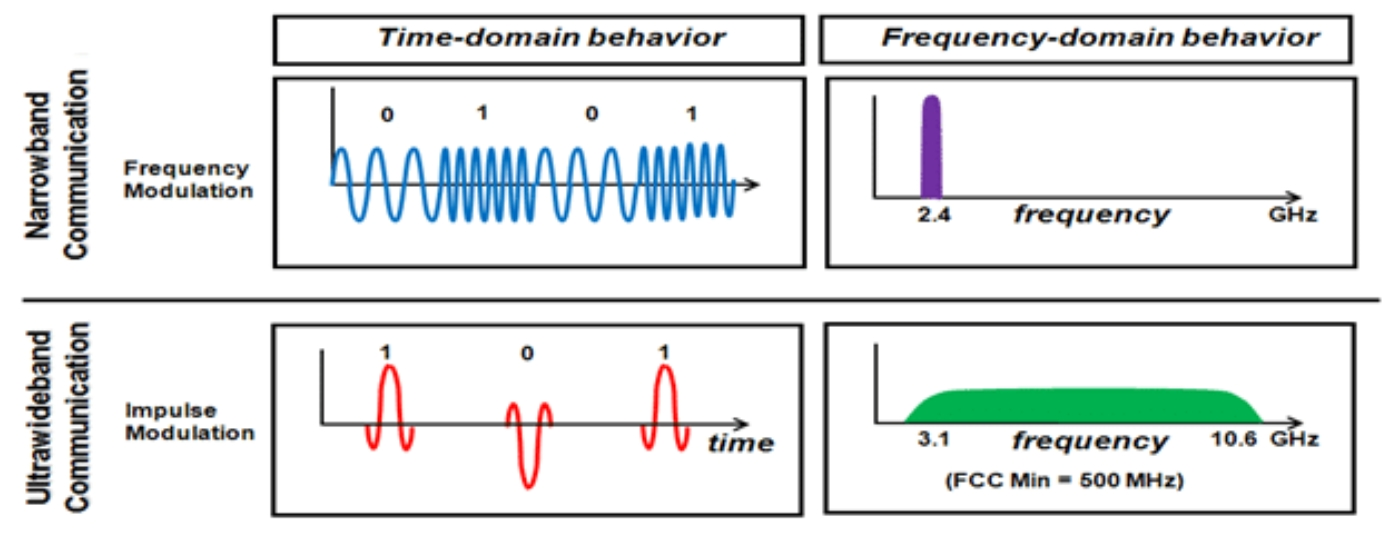
\includegraphics[width=0.8\textwidth]{image/section3/uwb.jpeg} 
    \caption[UWB Spectrum vs Narrowband]{UWB Spectrum vs Narrowband (\textbf{Nguồn:} \href{https://sirinsoftware.com/blog/uwb-technology-review-modules-characteristics-usage-perspectives}{Sirin Software})}
    \label{}
\end{figure}

\begin{table}[h]
\centering
\label{tab:uwb_specs}
\begin{tabular}{|l|l|}
\hline
\textbf{Thông số} & \textbf{Giá trị} \\ 
\hline
Băng tần hoạt động & 3.1--10.6 GHz (nhiều băng tần con) \\ 
Băng thông & > 500 MHz (thường 500--1000 MHz) \\ 
Phạm vi hoạt động & 10--200 m (trong nhà / ngoài trời) \\ 
Tốc độ dữ liệu & 110 kbps -- 27 Mbps \\ 
Độ chính xác định vị & 10--30 cm (thông thường), < 10 cm (tối ưu) \\ 
Công suất tiêu thụ & < 100 mW (điển hình) \\ 
Độ trễ & < 1 ms (cho đo khoảng cách) \\ 
Chuẩn hóa & IEEE 802.15.4a/z, FiRa Consortium \\ 
\hline
\end{tabular}
\caption{Thông số kỹ thuật của UWB}
\end{table}


\subsubsection{Nguyên lý hoạt động}

UWB truyền dữ liệu bằng cách phát các \textbf{xung vô tuyến cực ngắn} (\textit{Impulse radio pulses}) có độ rộng rất nhỏ (nhỏ hơn 1 ns) và chu kỳ hoạt động thấp, thay vì phát sóng liên tục (\textit{Continuous wave}) như Wi-Fi hoặc Bluetooth \cite{ghavami2007ultra}.


\begin{tabular}{ll}
a & Đạo hàm bậc năm của hàm Gaussian \\
b & Xung Gaussian đơn chu kỳ (Gaussian monocycle) \\
c & Xung Gaussian đơn chu kỳ sau khi qua bộ lọc \\
d & Phổ tương ứng được chuẩn hóa theo mặt nạ phổ FCC
\end{tabular}

\begin{figure}[H]
    \centering
    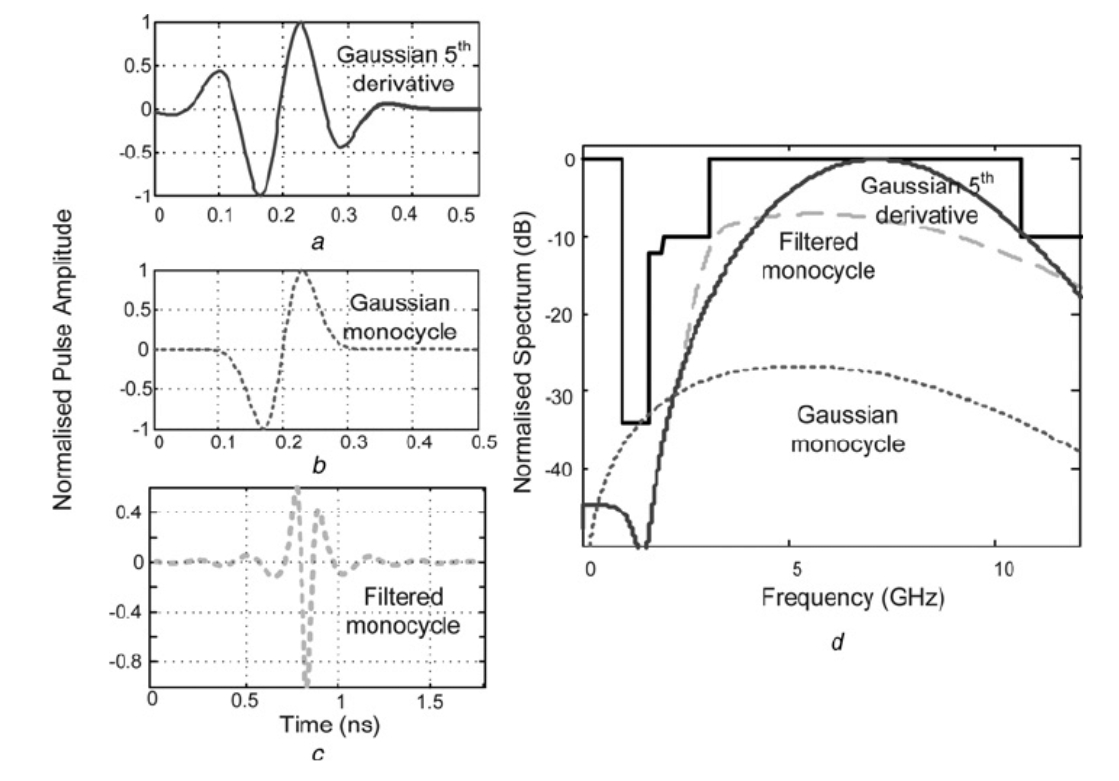
\includegraphics[width=0.8\textwidth]{image/section3/uwb2.jpeg} 
    \caption[Dạng sóng miền thời gian của xung UWB (Gaussian monocycle)]{Dạng sóng miền thời gian của xung UWB (Gaussian monocycle) (\textbf{Nguồn:} \href{https://www.researchgate.net/publication/260673659_Ultra-wideband_pulse_shaping_bypassing_the_inherent_limitations_of_the_Gaussian_monocycle}{ResearchGate})}
    \label{}
\end{figure}

\par\vspace{1em}
\textbf{Các đặc điểm quan trọng của công nghệ UWB bao gồm:}
\par\vspace{0.5em}
\textbf{1. Đo thời gian truyền sóng (TOF):}
\par\vspace{0.3em}
UWB có khả năng đo khoảng cách với độ chính xác cao dựa trên thời gian sóng điện từ truyền từ thiết bị phát đến thiết bị thu và quay trở lại. Khoảng cách được tính theo công thức:

\begin{equation}
d = \frac{c \cdot \Delta t}{2}
\end{equation}

Trong đó:
\begin{itemize}
    \item $d$: Khoảng cách giữa hai thiết bị (m)
    \item $c$: Tốc độ ánh sáng trong chân không ($3 \times 10^8$ m/s)
    \item $\Delta t$: Thời gian truyền hai chiều (\textit{Round-trip time}) (s)
\end{itemize}

Với độ chính xác đo thời gian ở mức khoảng 1 ns, UWB có thể đạt độ chính xác đo khoảng cách vào khoảng 30 cm. Các kỹ thuật nâng cao như đo dựa trên pha (\textit{Phase-based ranging}) hoặc chế độ chuỗi huấn luyện bảo mật (\textit{Scrambled Timestamp Sequence -- STS}) có thể cải thiện độ chính xác xuống dưới 10 cm \cite{decawave2017}.
\par\vspace{0.5em}
\textbf{2. Đo khoảng cách hai chiều đối xứng (DS-TWR):}
\par\vspace{0.3em}
Theo lý thuyết cơ bản, khoảng cách có thể được tính bằng phương pháp đo một vòng (Single-Sided TWR - SS-TWR) thông qua việc trao đổi hai gói tin. Tuy nhiên, SS-TWR gặp phải sai số rất lớn do sự trôi dạt xung nhịp (Clock drift) giữa bộ dao động thạch anh của hai thiết bị độc lập (điện thoại và ECU). Để khắc phục triệt để sai số này và tuân thủ chuẩn bảo mật CCC Digital Key Release 3.0, hệ thống bắt buộc sử dụng giao thức \textbf{Symmetrical Double-Sided Two-Way Ranging (DS-TWR)}.

Giao thức DS-TWR yêu cầu trao đổi 3 gói tin (\textit{Poll, Response, Final}) để tự động bù trừ sai lệch thời gian phần cứng. Trình tự thực hiện như sau:

\begin{enumerate}
    \item \textbf{Khởi tạo (Poll):} Thiết bị A (Initiator/Smartphone) phát gói \textit{Poll} và ghi nhận thời gian phát. Thiết bị B (Responder/ECU) nhận gói tin và ghi lại thời gian đến.
    \item \textbf{Phản hồi (Response):} Sau một khoảng thời gian trễ xử lý ($T_{reply1}$), Thiết bị B phát gói \textit{Response}. Thiết bị A nhận gói tin này và tính toán được thời gian truyền vòng đầu tiên ($T_{round1}$).
    \item \textbf{Chốt chặng (Final):} Sau khoảng thời gian trễ xử lý ($T_{reply2}$), Thiết bị A phát gói \textit{Final} mang theo dữ liệu về các mốc thời gian của nó. Thiết bị B nhận gói \textit{Final} và tính toán được thời gian truyền vòng thứ hai ($T_{round2}$).
\end{enumerate}

\begin{figure}[H]
    \centering
    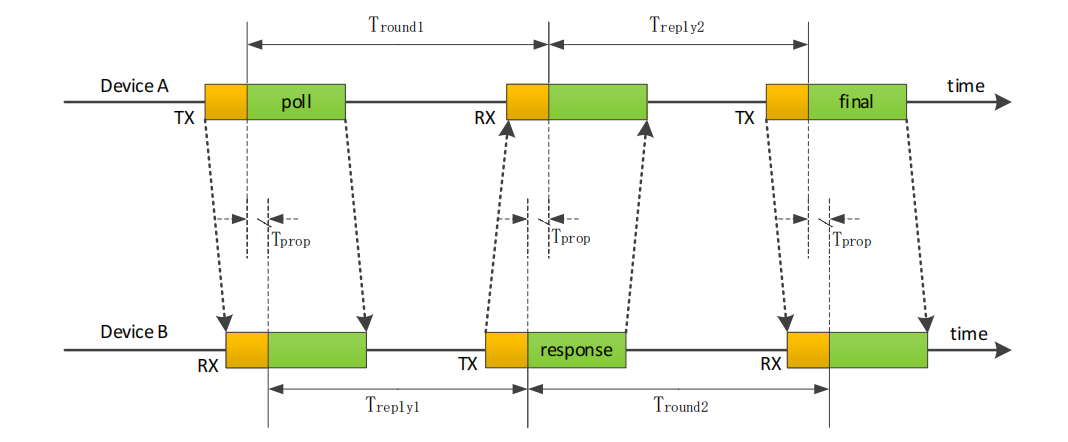
\includegraphics[width=0.7\textwidth]{image/section3/dstwr_protocol.png} 
    \caption[Sơ đồ trao đổi gói tin của giao thức Symmetrical DS-TWR]{Sơ đồ trao đổi gói tin của giao thức Symmetrical DS-TWR (\textbf{Nguồn:} \href{https://www.lansitec.com/uwb-positioning-technology/}{Lansitec})}
    \label{fig:dstwr_protocol}
\end{figure}

Thời gian truyền sóng thực sự (Time-of-Flight - ToF) được tính toán bằng công thức:
\begin{equation}
\text{ToF} = \frac{T_{round1} \times T_{round2} - T_{reply1} \times T_{reply2}}{T_{round1} + T_{round2} + T_{reply1} + T_{reply2}}
\end{equation}

Trong đó:
\begin{itemize}
    \item $T_{round1}$: Thời gian đo tại A, từ khi gửi \textit{Poll} đến khi nhận \textit{Response}.
    \item $T_{reply1}$: Thời gian xử lý tại B, từ khi nhận \textit{Poll} đến khi gửi \textit{Response}.
    \item $T_{round2}$: Thời gian đo tại B, từ khi gửi \textit{Response} đến khi nhận \textit{Final}.
    \item $T_{reply2}$: Thời gian xử lý tại A, từ khi nhận \textit{Response} đến khi gửi \textit{Final}.
\end{itemize}

Nhờ việc lấy tích chéo và chia cho tổng thời gian của cả hai vòng truyền, phương pháp DS-TWR triệt tiêu được hoàn toàn sai số bậc nhất (first-order error) sinh ra bởi sự chênh lệch tần số đồng hồ ($\Delta f$) giữa Smartphone và vi mạch UWB DW3000 trên xe. Điều này giúp hệ thống đạt được độ chính xác định vị ở mức centimet ($< 10$ cm) mà không cần chia sẻ chung một nguồn xung nhịp vật lý \cite{neirynck2016overview}.
\par\vspace{0.5em}

\textbf{3. Xác định góc đến của tín hiệu (AoA):}
\par\vspace{0.3em}
UWB có thể xác định góc đến của tín hiệu thông qua hệ thống nhiều anten (\textit{Antenna array}), cho phép thực hiện chức năng \textbf{xác định hướng} (\textit{Direction finding}) \cite{bharadwaj2020accurate}. Khi kết hợp với đo khoảng cách, hệ thống có thể thực hiện \textbf{định vị chính xác} (\textit{Precise positioning}) trong không gian ba chiều.

\subsubsection{Đo khoảng cách đa điểm (One-to-Many Ranging)}

Để định vị được thiết bị trong mặt phẳng quanh xe (như mục Định vị đa mỏ neo và Trilateration trình bày), hệ thống cần thu thập \textbf{đồng thời} nhiều khoảng cách $d_0, d_1, d_2$ từ một điện thoại đến nhiều mỏ neo trong \textbf{cùng một vòng đo} (ranging round). Việc lặp tuần tự nhiều phiên đo một–một (one-to-one DS-TWR) không đáp ứng được yêu cầu này vì hai lý do: (i) mỗi phiên DS-TWR riêng lẻ tiêu tốn một khoảng thời gian cố định nên tổng thời gian để đo lần lượt $N$ mỏ neo tăng tuyến tính theo $N$, làm giảm tần suất cập nhật vị trí; và (ii) các khoảng cách thu được tại các thời điểm khác nhau sẽ không đồng bộ về mặt thời gian, dẫn đến sai số đáng kể khi thiết bị đang chuyển động và làm suy giảm tính nhất quán của bài toán Trilateration.

Để giải quyết vấn đề trên, chuẩn FiRa (FiRa Consortium) định nghĩa các chế độ đo khoảng cách theo số lượng thiết bị tham gia trong một phiên \cite{fira_uwb_ranging}:
\begin{itemize}
    \item \textbf{One-to-One (O2O):} Một bộ khởi tạo (Initiator/Controller) đo khoảng cách với đúng một bộ đáp ứng (Responder/Controlee). Đây là chế độ cơ bản nhất, được dùng cho bài toán đo khoảng cách đơn lẻ.
    \item \textbf{One-to-Many (O2M):} Một bộ khởi tạo đo khoảng cách \textbf{đồng thời} với nhiều bộ đáp ứng (tối đa 8 responder trong một phiên theo đặc tả FiRa) \cite{qorvo_o2m}. Chế độ này còn được gọi là \textbf{DS-TWR multicast}, trong đó bộ khởi tạo phát một thông điệp khởi tạo và các responder lần lượt phản hồi trong các khe thời gian (slots) được phân bổ trước của cùng một vòng đo.
    \item \textbf{Many-to-Many (M2M):} Nhiều bộ khởi tạo đo khoảng cách với nhiều bộ đáp ứng trong cùng một phiên, phục vụ các ứng dụng quy mô lớn như định vị đội thiết bị trong nhà máy.
\end{itemize}

\par\vspace{0.5em}
\textbf{Nguyên lý hoạt động của DS-TWR multicast:}
\par\vspace{0.3em}
Trong chế độ O2M, điện thoại (Controller) phát một thông điệp khởi tạo vòng đo (\textit{Ranging Initiation Message} -- RIM) hướng tới tất cả các mỏ neo. Mỗi mỏ neo (Responder) sau đó phản hồi bằng một thông điệp đáp ứng (\textit{Ranging Response Message} -- RRM) trong khe thời gian riêng của nó, và Controller chốt vòng đo bằng thông điệp kết thúc (\textit{Ranging Final Message} -- RFM). Quá trình trao đổi ba gói tin \textit{Poll -- Response -- Final} vẫn tuân theo đúng giao thức DS-TWR đã trình bày, nhưng được ghép kênh theo thời gian (time-slotted) cho nhiều responder trong cùng một vòng đo, nhờ đó bộ khởi tạo thu được $N$ khoảng cách $d_0, d_1, \dots, d_{N-1}$ gần như đồng thời với chi phí thời gian chỉ tương đương một phiên đo \cite{neirynck2016overview,fira_uwb_ranging}.

\begin{figure}[H]
    \centering
    \begin{tikzpicture}[scale=0.9, every node/.style={font=\small}]
        % Initiator (controller)
        \node[draw, circle, fill=red!10, minimum size=1.7cm, align=center] (C) at (0,0) {Controller\\ \textit{(Phone)}};

        % Responders (anchors)
        \node[draw, circle, fill=blue!8, minimum size=1.4cm, align=center] (R0) at (0,2.7)   {Anchor $A_0$};
        \node[draw, circle, fill=blue!8, minimum size=1.4cm, align=center] (R1) at (-2.4,-1.4) {Anchor $A_1$};
        \node[draw, circle, fill=blue!8, minimum size=1.4cm, align=center] (R2) at (2.4,-1.4)  {Anchor $A_2$};

        % DS-TWR links
        \draw[<->, very thick, blue!60] (C) -- (R0) node[midway, right] {\scriptsize DS-TWR $d_0$};
        \draw[<->, very thick, blue!60] (C) -- (R1) node[midway, above left]  {\scriptsize DS-TWR $d_1$};
        \draw[<->, very thick, blue!60] (C) -- (R2) node[midway, above right] {\scriptsize DS-TWR $d_2$};

        \node[align=center, font=\scriptsize\itshape] at (0,-2.7) {Một vòng đo duy nhất -- ba khoảng cách\\ được thu thập đồng thời};
    \end{tikzpicture}
    \caption[Nguyên lý đo khoảng cách một–nhiều (One-to-Many Ranging)]{Nguyên lý đo khoảng cách \textbf{một–nhiều} (One-to-Many Ranging / DS-TWR multicast): một bộ khởi tạo (Controller -- điện thoại) thực hiện DS-TWR đồng thời với ba bộ đáp ứng (Anchor) trong cùng một vòng đo, thu được ba khoảng cách $d_0, d_1, d_2$ phục vụ giải thuật Trilateration.}
    \label{fig:one_to_many_ranging}
\end{figure}

\par\vspace{0.5em}
\textbf{Vai trò của O2M trong hệ thống định vị đa điểm:}
\par\vspace{0.3em}
Chế độ one-to-many chính là nền tảng cho kiến trúc định vị đa mỏ neo của đề tài: điện thoại chỉ cần duy trì một phiên UWB duy nhất nhưng vẫn thu được đồng thời ba khoảng cách $d_0, d_1, d_2$ để giải tọa độ $(x, y)$ bằng Trilateration. Trên hệ điều hành Android, chế độ này tương ứng với cấu hình \texttt{CONFIG\_MULTICAST\_DS\_TWR} trong API \texttt{androidx.core.uwb.RangingParameters} -- cấu hình \textit{one-to-many STATIC STS DS-TWR} với tần suất vòng đo khoảng 200\,ms và mỗi vòng đo phân bổ tối đa 20 khe thời gian cho các responder \cite{android_ranging}. Nhờ tính đồng bộ về thời gian của các khoảng cách, dữ liệu đầu vào cho bộ lọc Kalman và tầng quyết định truy cập luôn nhất quán về mặt hình học, tránh được hiện tượng lệch pha gây rung lắc quỹ đạo khi thiết bị di chuyển.

\subsubsection{Đo khoảng cách đồng thời (Concurrent Ranging)}

Bên cạnh chế độ one-to-many (O2M) chuẩn FiRa vừa trình bày --- vốn tách các phản hồi của các responder theo các khe thời gian riêng biệt trong cùng một vòng đo --- các nghiên cứu gần đây còn đề xuất một hướng tiếp cận triệt để hơn về mặt hiệu quả truyền thông: \textbf{đo khoảng cách đồng thời} (\textit{Concurrent Ranging}), được giới thiệu bởi Corbalán và Picco \cite{corbalan2020concurrent}. Kỹ thuật này cho phép bộ khởi tạo đo khoảng cách tới $N$ responder bằng đúng \textbf{hai gói tin} duy nhất, thay vì $2N$ gói tin của SS-TWR hay tối đa $4N$ gói tin của DS-TWR truyền thống, qua đó giảm mạnh chi phí mạng, độ trễ và năng lượng tiêu thụ trong khi vẫn giữ nguyên tần suất cập nhật vị trí.

\par\vspace{0.5em}
\textbf{Nguyên lý hoạt động:}
\par\vspace{0.3em}
Trong đo khoảng cách đồng thời, bộ khởi tạo phát duy nhất một gói \textit{poll} dạng \textbf{quảng bá} (broadcast). Khi nhận được poll, \textbf{tất cả} các responder trong phạm vi phủ sóng phản hồi \textbf{cùng lúc} --- thay vì lần lượt theo khe thời gian như DS-TWR multicast --- khiến các tín hiệu phản hồi chồng lấn lên nhau trên kênh truyền. Nhờ đặc tính xung cực ngắn (dưới $2$\,ns) của UWB, các đường truyền ứng với từng responder vẫn phân biệt được với nhau trong miền thời gian thông qua \textbf{đáp ứng xung kênh truyền} (\textit{Channel Impulse Response} -- CIR) mà vi mạch thu phát (DW1000/DW3000) cung cấp: chênh lệch khoảng cách giữa hai responder sinh ra độ dịch thời gian $\Delta t = \Delta d / c$ giữa hai đường đi trực tiếp (direct path) tương ứng, cho phép bộ khởi tạo ước lượng thời gian đến (Time of Arrival -- ToA) của từng tín hiệu và suy ra đồng thời nhiều khoảng cách $d_0, d_1, \dots, d_{N-1}$ \cite{corbalan2020concurrent}.

\begin{figure}[H]
    \centering
    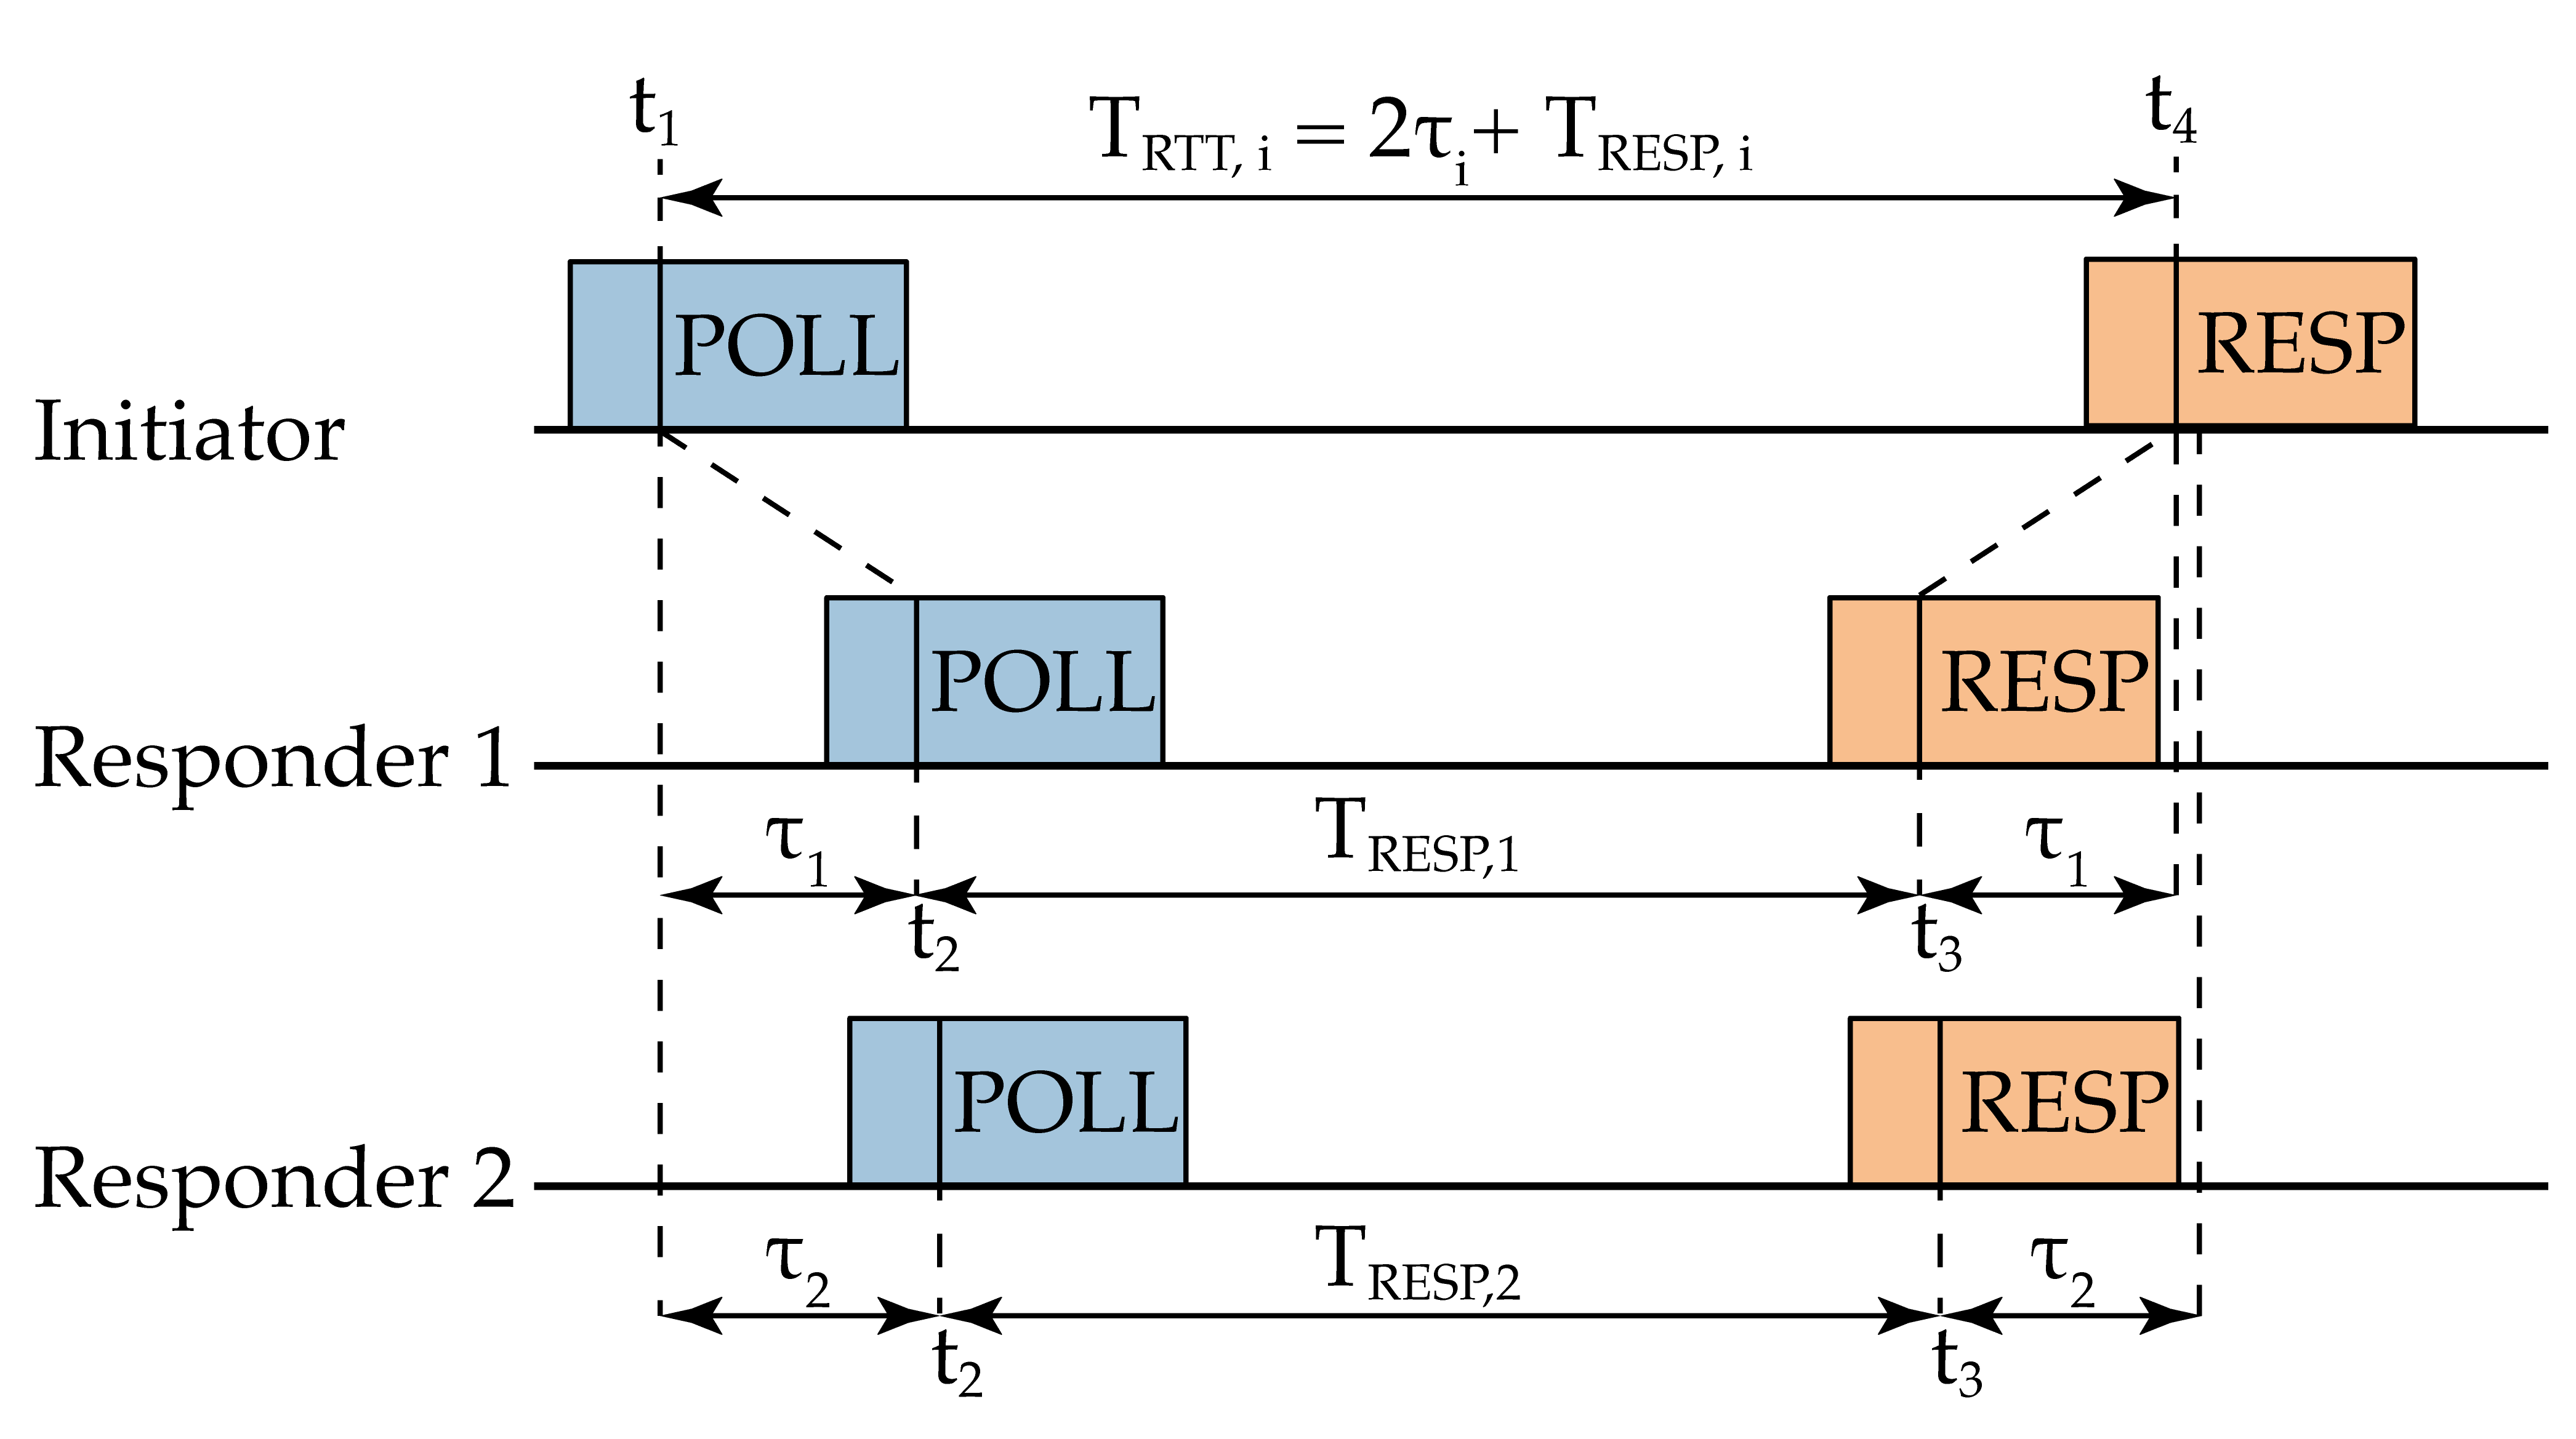
\includegraphics[width=0.55\textwidth]{image/section3/concurrent_ranging.png}
    \caption[Nguyên lý đo khoảng cách đồng thời (Concurrent Ranging)]{Nguyên lý đo khoảng cách đồng thời (Concurrent Ranging): bộ khởi tạo phát một gói poll quảng bá duy nhất, các responder phản hồi chồng lấn theo thời gian; các đường truyền được phân biệt qua đáp ứng xung kênh truyền (CIR). (\textbf{Nguồn:} Corbalán \& Picco, 2020 \cite{corbalan2020concurrent})}
    \label{fig:concurrent_ranging}
\end{figure}

\par\vspace{0.5em}
\textbf{Liên hệ với đề tài:}
\par\vspace{0.3em}
Đo khoảng cách đồng thời mở ra một hướng tối ưu quan trọng cho kiến trúc định vị đa mỏ neo của đề tài: nếu loại bỏ được nhu cầu giải mã từng gói phản hồi riêng lẻ và chỉ dựa vào CIR (vốn được vi mạch DW1000/DW3000 cung cấp sẵn cho tầng ứng dụng), chi phí mạng và năng lượng của một vòng đo $N$ mỏ neo có thể giảm đáng kể, đồng thời tăng tần suất cập nhật vị trí. Tuy nhiên, kỹ thuật này đặt ra các thách thức về độ chính xác lập lịch phát (TX scheduling) và nhận dạng responder mà hệ thống hiện tại chưa khai thác; do đó, trong phạm vi đề tài, nhóm lựa chọn chế độ DS-TWR multicast chuẩn FiRa (các responder trả lời tuần tự theo khe thời gian) để đảm bảo độ tin cậy và khả năng tích hợp với API chuẩn của hệ điều hành, đồng thời ghi nhận concurrent ranging như một định hướng nâng cấp tiềm năng trong tương lai.




%----------------------------------------------------------------------------------------------------




\subsubsection{Bảo mật UWB – Chống tấn công chuyển tiếp (Relay Attack)}

UWB là công nghệ truyền thông không dây hiếm hoi có khả năng \textbf{chống relay attack một cách hiệu quả} nhờ tận dụng các đặc tính bảo mật ở \textbf{lớp vật lý} (\textit{Physical layer security}).
\par\vspace{0.5em}
\textbf{1. Đo khoảng cách an toàn (Secure Ranging):}
\par\vspace{0.3em}
Chuẩn IEEE 802.15.4z giới thiệu cơ chế \textbf{UWB tốc độ cao} (High-Rate Pulse repetition – HRP) kết hợp với \textbf{chuỗi dấu thời gian xáo trộn} (Scrambled Timestamp Sequence – STS) nhằm ngăn chặn các cuộc tấn công chuyển tiếp và gây nhiễu \cite{ieee802154z}:

\begin{itemize}
    \item \textbf{STS:} Mỗi gói tin UWB chứa một chuỗi tiền tố (\textit{Preamble}) được xáo trộn và sinh ra từ khóa bí mật dùng chung. Kẻ tấn công không thể tự tạo hoặc chuyển tiếp một STS hợp lệ nếu không biết khóa.
    
    \item \textbf{Toàn vẹn dấu thời gian (Timestamp integrity):} Dấu thời gian đo khoảng cách được ràng buộc mật mã với nội dung gói tin, giúp phát hiện các hành vi thao túng thời gian truyền.
\end{itemize}
\par\vspace{0.5em}
\textbf{2. Các ràng buộc ở lớp vật lý:}
\par\vspace{0.3em}
\begin{itemize}
    \item \textbf{Giới hạn tốc độ ánh sáng:} Tín hiệu vô tuyến không thể truyền nhanh hơn vận tốc ánh sáng $c = 3 \times 10^8$ m/s. Nếu khoảng cách đo được nhỏ hơn khoảng cách vật lý thực tế, hệ thống có thể phát hiện hành vi relay.
    
    \item \textbf{Độ trễ rất thấp:} Quá trình đo khoảng cách bằng UWB có độ trễ nhỏ hơn 1 ms. Tấn công relay bắt buộc phải thêm độ trễ do xử lý và truyền lại tín hiệu, từ đó dễ bị phát hiện.
    
    \item \textbf{Khả năng chống đa đường truyền (Multipath resilience):} Các xung UWB cực ngắn cho phép phân biệt rõ đường truyền trực tiếp và các tín hiệu phản xạ, khiến việc giả mạo hoặc đánh lừa hệ thống trở nên rất khó khăn.
\end{itemize}

\subsubsection{Ứng dụng trong lĩnh vực ô tô}

Công nghệ UWB hiện đang được nhiều hãng ô tô lớn triển khai trong các hệ thống \textbf{chìa khóa kỹ thuật số} (Digital Key) nhờ khả năng đo khoảng cách chính xác và chống tấn công chuyển tiếp hiệu quả.
\par\vspace{0.5em}
\textbf{1. BMW Digital Key Plus (2020):}
\par\vspace{0.3em}
BMW ứng dụng công nghệ UWB sử dụng các chip dòng Trimension của NXP để thực hiện đo khoảng cách an toàn và xác định hướng tiếp cận của người dùng. Hệ thống cho phép mở khóa xe tự động khi người dùng đến gần mà không cần thao tác trên điện thoại, hay còn gọi là chế độ vào xe thụ động (\textit{Passive entry}).
\par\vspace{0.5em}
\textbf{2. Apple Car Key (iOS 14 trở lên):}
\par\vspace{0.3em}
Apple tích hợp UWB trên các thiết bị iPhone từ thế hệ iPhone 11 trở lên thông qua chip U1. Giải pháp này tuân theo chuẩn Digital Key Release 3.0 do Car Connectivity Consortium ban hành, cho phép xác thực và mở khóa xe với độ bảo mật cao.
\par\vspace{0.5em}
\textbf{3. Liên minh FiRa (FiRa Consortium):}
\par\vspace{0.3em}
FiRa Consortium là liên minh gồm nhiều tập đoàn công nghệ và ô tô lớn như Apple, Samsung, Google, BMW, Volkswagen, NXP và Qorvo, với mục tiêu xây dựng và chuẩn hóa công nghệ UWB cho các ứng dụng trong lĩnh vực ô tô, nhà thông minh và Internet vạn vật công nghiệp (Industrial IoT).

\begin{figure}[H]
    \centering
    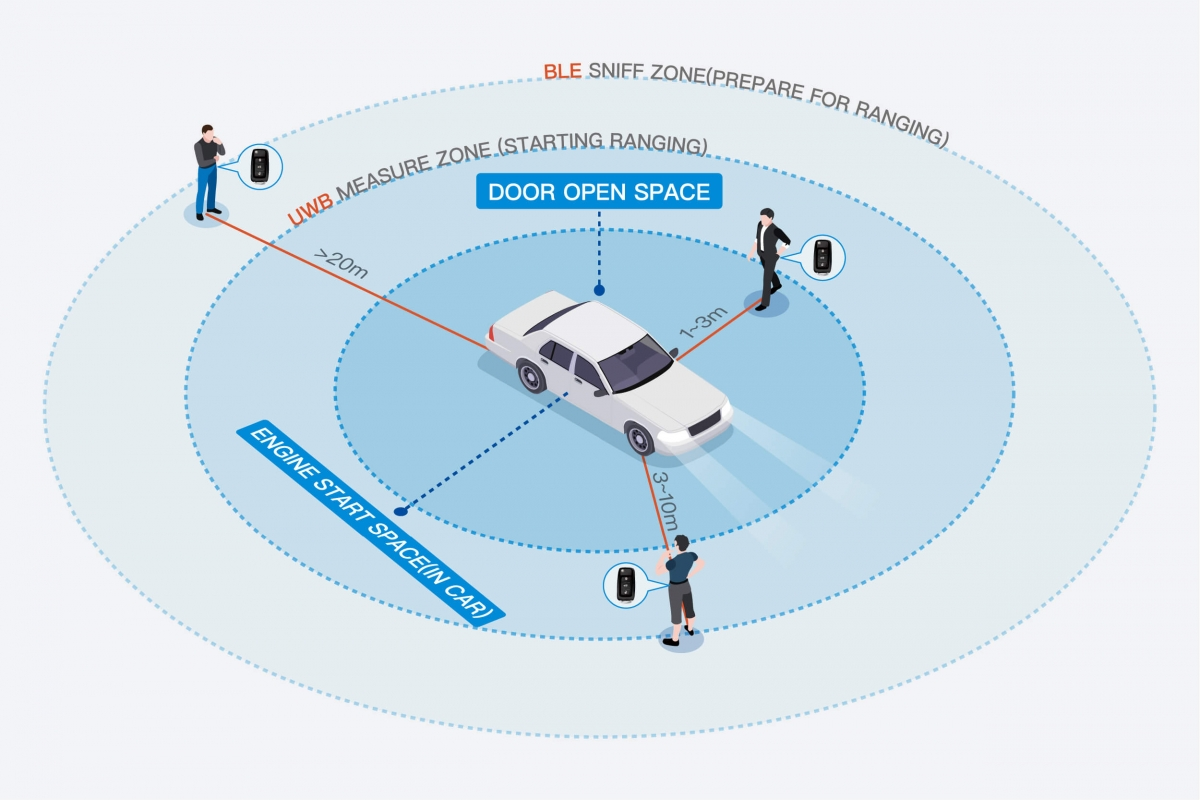
\includegraphics[width=0.8\textwidth]{image/section3/uwb4.jpg} 
    \caption[Vai trò của UWB trong hệ thống Digital Key]{Vai trò của UWB trong hệ thống Digital Key (\textbf{Nguồn:} \href{https://www.tsingcar.cn/en/business/}{TsingCar})}
    \label{fig:uwb_role}
\end{figure}



\subsection{Định vị đa mỏ neo và Trilateration}

\subsubsection{Giới hạn của kiến trúc đo khoảng cách đơn mỏ neo}

Trong giai đoạn một (Stage 1), hệ thống chỉ sử dụng duy nhất một mỏ neo (single anchor) UWB và do đó chỉ trích xuất được một giá trị khoảng cách vô hướng $d$ giữa điện thoại và xe. Về mặt hình học, một phép đo khoảng cách đơn lẻ chỉ cho biết thiết bị nằm đâu đó trên một \textbf{đường tròn} (trong không gian hai chiều) hoặc một \textbf{mặt cầu} (trong không gian ba chiều) bán kính $d$ bao quanh mỏ neo, mà không cung cấp bất kỳ thông tin nào về \textbf{hướng} (bearing) của thiết bị. Hệ quả trực tiếp là: hệ thống chỉ có thể trả lời câu hỏi \textit{``người dùng đang ở xa hay gần xe?''} (khoảng cách, 1D) mà không thể trả lời câu hỏi \textit{``người dùng đang đứng ở vị trí nào quanh xe?''} (tọa độ, 2D/3D).

Hạn chế này dẫn đến hai bất cập lớn đối với một hệ thống Smart Car Access thực thụ:
\begin{itemize}
    \item \textbf{Không thể định vị cục bộ:} Hệ thống không phân biệt được người dùng đang tiến về phía \textbf{cửa tài xế}, \textbf{cốp xe} hay \textbf{cửa phụ}, do đó không thể kích hoạt các chức năng mở khóa theo vùng (zone-based actuation) như ``mở cửa tài xế khi người dùng đến gần cột B bên trái'' hay ``mở cốp thông minh khi người dùng đứng sau đuôi xe''.
    \item \textbf{Nhạy cảm với nhiễu biên:} Quyết định mở khóa chỉ dựa trên một ngưỡng khoảng cách vô hướng ($d \le 2.0$m) rất dễ bị tác động bởi nhiễu đa đường (multipath) và nhiễu phi tuyến (NLOS), vì không có thông tin hình học nào để kiểm chứng chéo tính nhất quán của phép đo.
\end{itemize}

Để giải quyết triệt để bài toán trên, giai đoạn hai (Stage 2) nâng cấp hệ thống lên kiến trúc \textbf{định vị đa mỏ neo} (multi-anchor localization): bố trí \textbf{ba mỏ neo UWB} cố định trên thân xe, thu thập đồng thời ba khoảng cách $d_0, d_1, d_2$ và thực hiện \textbf{Trilateration} để giải ra tọa độ phẳng $(x, y)$ của thiết bị trong hệ quy chiếu gắn với xe, sau đó hợp nhất quỹ đạo bằng \textbf{Bộ lọc Kalman} hai chiều để ước lượng cả vị trí lẫn vận tốc $(x, y, v_x, v_y)$.

\subsubsection{Nguyên lý Trilateration}

Trilateration là kỹ thuật định vị dựa trên việc giao cắt các mặt hình học khoảng cách. Xét một tập $n$ mỏ neo có tọa độ đã biết $\mathbf{a}_i = (x_i, y_i)$ (trong hệ quy chiếu xe) và thiết bị cần định vị có tọa độ chưa biết $\mathbf{p} = (x, y)$. Khoảng cách đo được từ thiết bị đến mỏ neo thứ $i$ là $d_i$. Với giả thiết các mỏ neo và thiết bị cùng nằm trên một mặt phẳng ngang (độ cao xấp xỉ bằng nhau), ta có hệ phương trình phi tuyến:

\begin{equation}
    \lVert \mathbf{p} - \mathbf{a}_i \rVert = \sqrt{(x - x_i)^2 + (y - y_i)^2} = d_i, \qquad i = 0, 1, \dots, n-1
\end{equation}

Ý nghĩa hình học của từng phương trình:
\begin{itemize}
    \item \textbf{Một mỏ neo:} Tập nghiệm là một đường tròn tâm $\mathbf{a}_0$ bán kính $d_0$ --- vô số vị trí khả dĩ (bài toán 1D, không xác định được hướng).
    \item \textbf{Hai mỏ neo:} Giao của hai đường tròn cho tối đa \textbf{hai} nghiệm đối xứng nhau qua đoạn thẳng nối hai tâm --- bài toán vẫn còn tính lưỡng trị (ambiguity).
    \item \textbf{Ba mỏ neo (không thẳng hàng):} Giao của ba đường tròn xác định \textbf{duy nhất một điểm} trên mặt phẳng --- đây là cấu hình tối thiểu để định vị 2D không lưỡng trị.
\end{itemize}

\begin{figure}[H]
    \centering
    \begin{tikzpicture}[scale=0.52, every node/.style={font=\small}]
        \coordinate (A0) at (0,3.0);
        \coordinate (A1) at (-2.598,-1.5);
        \coordinate (A2) at (2.598,-1.5);
        \coordinate (P)  at (0,0);

        \draw[blue!55, very thick, fill=blue!6, fill opacity=0.55] (A0) circle (3.0);
        \draw[blue!55, very thick, fill=blue!5, fill opacity=0.45] (A1) circle (3.0);
        \draw[blue!55, very thick, fill=blue!5, fill opacity=0.45] (A2) circle (3.0);

        \draw[dashed, gray] (A0) -- (P);
        \draw[dashed, gray] (A1) -- (P);
        \draw[dashed, gray] (A2) -- (P);

        \filldraw[red!70] (A0) circle (4pt) node[above=3pt] {$A_0(x_0,y_0)$};
        \filldraw[red!70] (A1) circle (4pt) node[below left=3pt] {$A_1(x_1,y_1)$};
        \filldraw[red!70] (A2) circle (4pt) node[below right=3pt] {$A_2(x_2,y_2)$};

        \node at (0.5,1.55) {$d_0$};
        \node at (-1.45,-0.85) {$d_1$};
        \node at (1.45,-0.85) {$d_2$};

        \filldraw[green!55!black] (P) circle (4pt) node[below=4pt] {$P(x,y)$};
    \end{tikzpicture}
    \caption[Nguyên lý Trilateration với ba mỏ neo]{Nguyên lý Trilateration: giao của ba đường tròn bán kính $d_0, d_1, d_2$ (tâm là ba mỏ neo $A_0, A_1, A_2$) xác định duy nhất vị trí $P(x,y)$ của thiết bị.}
    \label{fig:trilateration_principle}
\end{figure}

\textbf{Mở rộng sang không gian ba chiều:} Trong trường hợp tổng quát, mỗi phép đo $d_i$ mô tả một \textbf{mặt cầu} bán kính $d_i$ trong không gian 3D, và cần tối thiểu \textbf{bốn} mỏ neo không đồng phẳng để giải ra tọa độ $(x, y, z)$ một cách duy nhất. Trong phạm vi đề tài, các mỏ neo được gắn trên cùng một mặt phẳng ngang của thân xe và bài toán điều khiển truy cập chỉ cần đến tọa độ mặt phẳng $(x, y)$ (độ cao thiết bị cầm tay được xem là hằng số), do đó hệ ba phương trình mặt cầu được rút gọn về hệ ba phương trình đường tròn nêu trên. Công thức và thuật toán trình bày dưới đây hoàn toàn có thể mở rộng lên ba chiều bằng cách bổ sung thêm biến $z$ và ít nhất một mỏ neo thứ tư \cite{murphy1995trilateration}.

\subsubsection{Nghiệm đại số tuyến tính (Linear Least Squares)}

Để giải hệ phương trình phi tuyến trên một cách hiệu quả trên vi điều khiển, bước đầu tiên là \textbf{tuyến tính hóa} bằng phép trừ phương trình. Bình phương hai vế của từng phương trình:

\begin{equation}
    (x - x_i)^2 + (y - y_i)^2 = d_i^2
\end{equation}

Khai triển và trừ phương trình thứ $i$ cho một phương trình tham chiếu (chọn mỏ neo $A_0$):

\begin{equation}
    -2x(x_i - x_0) - 2y(y_i - y_0) = d_i^2 - d_0^2 - (x_i^2 + y_i^2) + (x_0^2 + y_0^2)
\end{equation}

Viết lại dưới dạng ma trận $\mathbf{A}\mathbf{p} = \mathbf{b}$:

\begin{equation}
    \mathbf{A} =
    \begin{bmatrix}
        x_1 - x_0 & y_1 - y_0 \\
        x_2 - x_0 & y_2 - y_0 \\
        \vdots & \vdots \\
        x_{n-1} - x_0 & y_{n-1} - y_0
    \end{bmatrix}, \qquad
    \mathbf{b} = -\frac{1}{2}
    \begin{bmatrix}
        d_1^2 - d_0^2 - \lVert \mathbf{a}_1 \rVert^2 + \lVert \mathbf{a}_0 \rVert^2 \\
        d_2^2 - d_0^2 - \lVert \mathbf{a}_2 \rVert^2 + \lVert \mathbf{a}_0 \rVert^2 \\
        \vdots
    \end{bmatrix}
\end{equation}

Với ba mỏ neo, hệ gồm hai phương trình độc lập và hai ẩn số, giải trực tiếp bằng phép nghịch đảo. Trong trường hợp có nhiều hơn ba mỏ neo (hệ quá xác định --- overdetermined), nghiệm bình phương tối thiểu (Least Squares) được tính bằng công thức chuẩn tắc:

\begin{equation}
    \hat{\mathbf{p}} = (\mathbf{A}^T \mathbf{A})^{-1} \mathbf{A}^T \mathbf{b}
\end{equation}

Nghiệm đại số này đóng vai trò \textbf{hạt giống khởi tạo} (initial seed) cho bước tối ưu phi tuyến bên dưới, giúp vòng lặp hội tụ nhanh và tránh rơi vào cực tiểu cục bộ sai.

\subsubsection{Trường hợp hai mỏ neo và sự lưỡng trị}

Khi chỉ có hai mỏ neo hợp lệ (ví dụ một mỏ neo bị mất gói tin hoặc nhiễu nặng), giao của hai đường tròn cho hai nghiệm đối xứng. Đặt $D = \lVert \mathbf{a}_1 - \mathbf{a}_0 \rVert$ là khoảng cách giữa hai tâm. Tồn tại nghiệm khi và chỉ khi bất đẳng thức tam giác được thỏa mãn: $|d_0 - d_1| \le D \le d_0 + d_1$. Khi đó:
\begin{itemize}
    \item \textbf{Nếu $D = d_0 + d_1$ hoặc $D = |d_0 - d_1|$:} Hai đường tròn tiếp xúc tại đúng một điểm.
    \item \textbf{Nếu các đường tròn không giao nhau (do nhiễu):} Thuật toán suy biến về điểm nằm trên đoạn thẳng nối hai tâm, tỷ lệ theo trọng số khoảng cách, đảm bảo luôn trả về một ước lượng hợp lý thay vì báo lỗi.
\end{itemize}

Trong hệ thống thực tế, hai nghiệm lưỡng trị được giải quyết bằng cách dùng \textbf{ước lượng vị trí của chu kỳ trước} (do bộ lọc Kalman duy trì) làm tham chiếu để chọn nghiệm gần nhất, hoặc bỏ qua khung dữ liệu đó nếu độ tin cậy thấp.

\subsubsection{Phương pháp Gauss-Newton}

Nghiệm tuyến tính hóa ở trên bỏ qua thành phần bậc hai nên có thể thiếu chính xác khi nhiễu lớn. Do đó, hệ thống sử dụng thêm một vòng lặp \textbf{Gauss-Newton} để tối ưu phi tuyến. Định nghĩa vector thặng dư (residual):

\begin{equation}
    \mathbf{r}(\mathbf{p}) =
    \begin{bmatrix}
        \lVert \mathbf{p} - \mathbf{a}_0 \rVert - d_0 \\
        \lVert \mathbf{p} - \mathbf{a}_1 \rVert - d_1 \\
        \lVert \mathbf{p} - \mathbf{a}_2 \rVert - d_2
    \end{bmatrix}
\end{equation}

Mục tiêu là cực tiểu hóa hàm chi phí bình phương tối thiểu phi tuyến $f(\mathbf{p}) = \tfrac{1}{2} \lVert \mathbf{r}(\mathbf{p}) \rVert^2$. Ma trận Jacobian của vector thặng dư theo $\mathbf{p}$:

\begin{equation}
    \mathbf{J}(\mathbf{p}) =
    \begin{bmatrix}
        \dfrac{x - x_0}{\lVert \mathbf{p} - \mathbf{a}_0 \rVert} & \dfrac{y - y_0}{\lVert \mathbf{p} - \mathbf{a}_0 \rVert} \\[1.2em]
        \dfrac{x - x_1}{\lVert \mathbf{p} - \mathbf{a}_1 \rVert} & \dfrac{y - y_1}{\lVert \mathbf{p} - \mathbf{a}_1 \rVert} \\[1.2em]
        \dfrac{x - x_2}{\lVert \mathbf{p} - \mathbf{a}_2 \rVert} & \dfrac{y - y_2}{\lVert \mathbf{p} - \mathbf{a}_2 \rVert}
    \end{bmatrix}
\end{equation}

Mỗi bước lặp cập nhật nghiệm theo phương trình chuẩn tắc:

\begin{equation}
    \mathbf{p}^{(k+1)} = \mathbf{p}^{(k)} - \left(\mathbf{J}^T \mathbf{J}\right)^{-1} \mathbf{J}^T\, \mathbf{r}(\mathbf{p}^{(k)})
\end{equation}

Vòng lặp kết thúc khi bước dịch chuyển nhỏ hơn ngưỡng hội tụ hoặc đạt số lần lặp tối đa (trong đề tài giới hạn 10 vòng). Điểm khởi tạo $\mathbf{p}^{(0)}$ được lấy từ nghiệm tuyến tính ở trên hoặc từ vị trí ước lượng của chu kỳ trước. Bên cạnh tọa độ, thuật toán còn trả về \textbf{giá trị RMS của thặng dư}:

\begin{equation}
    \text{RMS} = \sqrt{\frac{1}{n}\sum_{i=0}^{n-1} \left(\lVert \hat{\mathbf{p}} - \mathbf{a}_i \rVert - d_i\right)^2}
\end{equation}

Đại lượng RMS này là một thước đo \textbf{chất lượng lời giải} (fix quality): RMS nhỏ cho thấy ba khoảng cách nhất quán về mặt hình học, trong khi RMS lớn là dấu hiệu của nhiễu đa đường, che khuất tầm nhìn (NLOS) hoặc dữ liệu nhiễu. Giá trị này được nạp trực tiếp vào ma trận hiệp phương sai nhiễu đo $R$ của bộ lọc Kalman ở mục tiếp theo, giúp bộ lọc \textbf{tự động giảm mức tin cậy} đối với các khung dữ liệu kém chất lượng.

\subsubsection{Độ suy giảm chính xác hình học (GDOP)}

Độ chính xác của kết quả định vị không chỉ phụ thuộc vào nhiễu của phép đo khoảng cách mà còn phụ thuộc mạnh vào \textbf{hình học bố trí} của các mỏ neo. Mối quan hệ này được lượng hóa bằng chỉ số \textbf{Geometric Dilution of Precision (GDOP)} \cite{langley1999gdop}: cùng một mức nhiễu khoảng cách, nếu các mỏ neo bố trí gần như thẳng hàng hoặc cụm sát nhau, sai số vị trí sẽ bị \textbf{khuếch đại} lên rất lớn, đặc biệt tại các vùng nằm xa tam giác mỏ neo. Ngược lại, một cấu hình tam giác bao trùm vùng hoạt động sẽ cho GDOP thấp và sai số được kiểm soát \cite{ridolfi2018analysis}.

Trong đề tài, ba mỏ neo được bố trí theo một tam giác không thẳng hàng ôm lấy thân xe (Hình \ref{fig:anchor_geometry}): $A_0$ ở trung tâm cản sau, $A_1$ ở bên phải thân xe và $A_2$ ở cột B bên trái (đồng thời là điểm mở khóa cửa tài xế). Cấu hình này đảm bảo GDOP thấp ngay tại vùng cửa tài xế --- vùng quyết định mở khóa quan trọng nhất --- đồng thời hạn chế sai số tại vùng cốp xe.

\begin{figure}[H]
    \centering
    \begin{tikzpicture}[scale=0.72, every node/.style={font=\small}]
        % Car body (X right, Y forward)
        \draw[fill=gray!12, thick] (-1.0,-2.0) rectangle (1.0,2.0);
        \node[gray!70] at (0,0.0) {\textit{Thân xe}};

        % Coordinate axes
        \draw[->, thick] (0,-2.6) -- (0,2.9) node[above] {$y$ (tiến)};
        \draw[->, thick] (-1.7,0) -- (1.6,0) node[right] {$x$ (phải)};

        % Anchors
        \filldraw[red!70] (0,-2.0)  circle (3.5pt) node[below=3pt] {$A_0\,(0,\,-2.0)$};
        \filldraw[red!70] (0.95,0)  circle (3.5pt) node[right=3pt] {$A_1\,(0.95,\,0)$};
        \filldraw[red!70] (-0.95,0) circle (3.5pt) node[left=3pt]  {$A_2\,(-0.95,\,0)$};

        % Unlock point (driver door B-pillar = A2)
        \filldraw[green!55!black] (-0.95,0) circle (3.5pt);
        \node[green!45!black, right=3pt, align=left] at (-0.95,0.15) {Điểm mở khóa\\ (cửa tài xế)};
    \end{tikzpicture}
    \caption[Hệ tọa độ xe và bố trí ba mỏ neo UWB]{Hệ tọa độ gắn với xe và bố trí ba mỏ neo UWB: $A_0$ (trung tâm cản sau), $A_1$ (bên phải thân xe), $A_2$ (cột B bên trái --- đồng thời là điểm mở khóa cửa tài xế). Đơn vị: mét.}
    \label{fig:anchor_geometry}
\end{figure}

\subsection{Bộ lọc Kalman hai chiều (EKF) cho bám quỹ đạo}

Dữ liệu tọa độ $(x, y)$ thu được từ Trilateration vẫn chứa các thành phần nhiễu trắng và nhiễu do hiện tượng phản xạ đa đường (multipath), đặc biệt là các ``bước nhảy'' vị trí khi tín hiệu bị che khuất (NLOS). Nếu sử dụng trực tiếp kết quả thô, hệ thống sẽ gặp hiện tượng dao động (chattering) khi ra quyết định mở cửa. Bộ lọc Kalman --- được phát triển bởi Rudolf E. Kalman năm 1960 \cite{kalman1960} --- là một thuật toán ước lượng trạng thái tối ưu theo đệ quy cho các hệ thống tuyến tính chịu tác động của nhiễu Gauss \cite{welch2001kalman}. Trong đề tài, bộ lọc được sử dụng để \textbf{hợp nhất} chuỗi tọa độ đo từ Trilateration thành quỹ đạo mượt, đồng thời ước lượng cả vector vận tốc $(v_x, v_y)$ phục vụ cho cổng logic hướng tiếp cận (approach gate) ở tầng quyết định truy cập.

\textbf{Lưu ý về tính phi tuyến:} Phép đo khoảng cách $\rightarrow$ tọa độ vốn là bài toán phi tuyến, nhưng phần phi tuyến đã được xử lý triệt để ngay tại tầng Trilateration (Gauss-Newton). Do đó, tầng lọc chỉ làm việc với quan hệ đo tuyến tính $z = Hx + v$ và mô hình vận tốc hằng tuyến tính; bộ lọc Kalman mở rộng (Extended Kalman Filter) trong trường hợp này suy biến về đúng bộ lọc Kalman tuyến tính chuẩn.

\subsubsection{Mô hình trạng thái}

Vector trạng thái gồm bốn thành phần:

\begin{equation}
    \mathbf{x}_k = \begin{bmatrix} p_x & p_y & v_x & v_y \end{bmatrix}^T
\end{equation}

trong đó $(p_x, p_y)$ là vị trí (mét) và $(v_x, v_y)$ là vận tốc (mét/giây) của thiết bị trong hệ quy chiếu xe. Giả thiết chuyển động của người đi bộ được mô tả bởi mô hình \textbf{vận tốc hằng} (constant velocity) với nhiễu gia tốc ngẫu nhiên (manoeuvre noise):

\begin{equation}
    \mathbf{x}_{k} = \mathbf{F}(\Delta t)\, \mathbf{x}_{k-1} + \mathbf{w}_{k-1}, \qquad
    \mathbf{F}(\Delta t) =
    \begin{bmatrix}
        1 & 0 & \Delta t & 0 \\
        0 & 1 & 0 & \Delta t \\
        0 & 0 & 1 & 0 \\
        0 & 0 & 0 & 1
    \end{bmatrix}
\end{equation}

với $\Delta t$ là khoảng thời gian giữa hai chu kỳ xử lý, $\mathbf{w} \sim \mathcal{N}(0, \mathbf{Q})$ là nhiễu quá trình. Sử dụng mô hình nhiễu gia tốc trắng liên tục với cường độ $\sigma_a$, ma trận hiệp phương sai nhiễu quá trình có dạng:

\begin{equation}
    \mathbf{Q} = \sigma_a^2
    \begin{bmatrix}
        \tfrac{\Delta t^4}{4} & 0 & \tfrac{\Delta t^3}{2} & 0 \\[0.3em]
        0 & \tfrac{\Delta t^4}{4} & 0 & \tfrac{\Delta t^3}{2} \\[0.3em]
        \tfrac{\Delta t^3}{2} & 0 & \Delta t^2 & 0 \\[0.3em]
        0 & \tfrac{\Delta t^3}{2} & 0 & \Delta t^2
    \end{bmatrix}
\end{equation}

\subsubsection{Mô hình đo lường}

Phép đo ở mỗi chu kỳ là tọa độ $(x_{meas}, y_{meas})$ do Trilateration trả về:

\begin{equation}
    \mathbf{z}_k = \begin{bmatrix} x_{meas} \\ y_{meas} \end{bmatrix} = \mathbf{H}\, \mathbf{x}_k + \mathbf{v}_k, \qquad
    \mathbf{H} = \begin{bmatrix} 1 & 0 & 0 & 0 \\ 0 & 1 & 0 & 0 \end{bmatrix}, \qquad \mathbf{v} \sim \mathcal{N}(0, \mathbf{R})
\end{equation}

Ma trận hiệp phương sai nhiễu đo được xây dựng từ chất lượng lời giải Trilateration:

\begin{equation}
    \mathbf{R} = \sigma_{meas}^2 \, \mathbf{I}_{2\times 2}, \qquad
    \sigma_{meas} = \operatorname{clamp}(\text{RMS},\; 0.05,\; 1.0)
\end{equation}

Việc ràng buộc $\sigma_{meas}$ trong khoảng $[0.05,\,1.0]$ m đảm bảo bộ lọc không bao giờ tin tưởng mù quáng một khung dữ liệu ``quá tốt'' (nhiều khả năng là ngẫu nhiên) và cũng không loại bỏ hoàn toàn một khung dữ liệu nhiễu lớn.

\subsubsection{Hai giai đoạn của bộ lọc}

\paragraph*{A. Giai đoạn dự báo (Time Update / Predict)}

\begin{align}
    \hat{\mathbf{x}}_{k|k-1} &= \mathbf{F}(\Delta t)\, \hat{\mathbf{x}}_{k-1|k-1} \\
    \mathbf{P}_{k|k-1} &= \mathbf{F}\, \mathbf{P}_{k-1|k-1}\, \mathbf{F}^T + \mathbf{Q}
\end{align}

Giai đoạn dự báo được thực thi ở một nhịp cố định \textbf{10 Hz} ($\Delta t = 100$ ms), độc lập với nhịp nhận dữ liệu thô từ cầu nối (bridge). Điều này mang lại hai lợi ích: (i) đồng hồ ra quyết định mở khóa được giữ ổn định; (ii) khi một vài khung dữ liệu bị mất (dropped frames), bộ lọc vẫn \textbf{dự báo bù} (coasting) để lấp đầy khoảng trống quỹ đạo, miễn là khoảng trống không vượt quá ngưỡng cho phép (trong đề tài là 2 giây; nếu quá ngưỡng, quỹ đạo được khởi tạo lại từ đầu).

\paragraph*{B. Giai đoạn cập nhật (Measurement Update / Correct)}

Khi nhận được phép đo mới $\mathbf{z}_k$, bộ lọc tính toán:
\begin{itemize}
    \item \textbf{Vector đổi mới (Innovation):}
    \begin{equation}
        \tilde{\mathbf{y}}_k = \mathbf{z}_k - \mathbf{H}\, \hat{\mathbf{x}}_{k|k-1}
    \end{equation}
    \item \textbf{Ma trận hiệp phương sai đổi mới:}
    \begin{equation}
        \mathbf{S}_k = \mathbf{H}\, \mathbf{P}_{k|k-1}\, \mathbf{H}^T + \mathbf{R}
    \end{equation}
    \item \textbf{Độ lợi Kalman (Kalman Gain):}
    \begin{equation}
        \mathbf{K}_k = \mathbf{P}_{k|k-1}\, \mathbf{H}^T\, \mathbf{S}_k^{-1}
    \end{equation}
    \item \textbf{Cập nhật trạng thái ước lượng:}
    \begin{equation}
        \hat{\mathbf{x}}_{k|k} = \hat{\mathbf{x}}_{k|k-1} + \mathbf{K}_k\, \tilde{\mathbf{y}}_k
    \end{equation}
    \item \textbf{Cập nhật hiệp phương sai sai số:}
    \begin{equation}
        \mathbf{P}_{k|k} = (\mathbf{I} - \mathbf{K}_k\, \mathbf{H})\, \mathbf{P}_{k|k-1}
    \end{equation}
\end{itemize}

\paragraph*{C. Cổng lọc đổi mới (Innovation Gating)}

Để chống lại các xung nhiễu NLOS/multipath khiến tọa độ đo bị ``nhảy vọt'' xa khỏi quỹ đạo dự báo, bộ lọc áp dụng cơ chế \textbf{lọc ngưỡng đổi mới} (innovation gating): nếu chuẩn của vector đổi mới vượt quá bội số $k$ của độ lệch chuẩn dự báo ($\lVert \tilde{\mathbf{y}}_k \rVert > k\, \sqrt{\operatorname{tr}(\mathbf{S}_k)}$), phép đo được hạ cấp hoặc bỏ qua trong chu kỳ đó. Cơ chế này giúp quỹ đạo bám mượt ngay cả khi người dùng đi qua vùng che khuất, đồng thời vẫn giữ được phản hồi nhanh khi chuyển động là hợp lý.

\subsubsection{Cấu hình tham số thực nghiệm}

Hiệu quả của bộ lọc phụ thuộc vào việc cân bằng giữa hai ma trận $\mathbf{Q}$ (nhiễu quá trình) và $\mathbf{R}$ (nhiễu đo). Trong thực nghiệm triển khai trên ESP32-S3, cường độ nhiễu gia tốc được chọn $\sigma_a = 1.2$ m/s$^2$ --- đủ lớn để bộ lọc bám theo sự đổi hướng đột ngột của người đi bộ, nhưng đủ nhỏ để làm mượt nhiễu đo:
\begin{itemize}
    \item Nếu chọn $\mathbf{Q}$ lớn và $\mathbf{R}$ nhỏ: Bộ lọc tin vào cảm biến hơn, đáp ứng nhanh với thay đổi nhưng quỹ đạo bị nhiễu và dễ bị kéo lệch bởi xung NLOS.
    \item Nếu chọn $\mathbf{Q}$ nhỏ và $\mathbf{R}$ lớn: Bộ lọc tin vào mô hình chuyển động hơn, quỹ đạo rất mượt nhưng trễ (lag) so với bước đi thực tế và phản ứng chậm khi người dùng đổi hướng.
\end{itemize}

Dựa trên đặc tính chuyển động của con người (tốc độ đi bộ $\approx 1.2$ m/s) và nhịp xử lý 10Hz, bộ tham số trên đã được tinh chỉnh để quỹ đạo $(x, y)$ và vận tốc $(v_x, v_y)$ vừa mượt mà vừa phản hồi kịp thời, làm đầu vào cho tầng quyết định truy cập hình học (geometric access control) ở giai đoạn hai.



\subsection{Triển khai UWB – Phần cứng trong hệ thống}

\textbf{Trong đề tài này:} Công nghệ UWB đã được \textbf{hiện thực hóa hoàn toàn} và đóng vai trò là chốt chặn bảo mật vật lý cốt lõi của hệ thống. Sự kết hợp giữa vi điều khiển ESP32-S3 và \textbf{ba mỏ neo UWB} (sử dụng vi mạch tiêu chuẩn DW3000) giúp hệ thống đo lường khoảng cách theo thời gian thực (Real-time Secure Ranging), đồng thời hợp nhất ba khoảng cách thành tọa độ phẳng $(x, y)$ để định vị không gian (Real-time Localization).

Việc triển khai UWB thực tế giải quyết triệt để các hạn chế của bảo mật BLE thông thường:
\begin{itemize}
    \item \textbf{Đo khoảng cách chính xác (ToF):} Xác minh người dùng đang thực sự ở cạnh xe (với sai số chỉ ở mức centimet) thay vì chỉ dựa vào cường độ tín hiệu RSSI vốn dễ bị làm giả.
    \item \textbf{Định vị đa mỏ neo (Trilateration):} Xác định vị trí tương đối $(x, y)$ của người dùng quanh xe, làm nền tảng cho việc kích hoạt mở khóa theo vùng (cửa tài xế, cốp xe) thay vì chỉ so sánh một ngưỡng khoảng cách đơn lẻ.
    \item \textbf{Bảo vệ bằng STS (Scrambled Timestamp Sequence):} Kích hoạt cơ chế mã hóa xung UWB ở lớp vật lý, giúp loại bỏ hoàn toàn rủi ro tấn công tiếp sóng (Relay Attack).
\end{itemize}

\begin{table}[h]
\centering
\label{tab:uwb_chips}
\begin{tabular}{|l|l|l|l|}
\hline
\textbf{Vi mạch} & \textbf{Nhà sản xuất} & \textbf{Chuẩn IEEE} & \textbf{Ứng dụng trong đề tài} \\
\hline
DW3000 & Qorvo (Decawave) & 802.15.4a/z & Vi mạch thu phát cho ba mỏ neo UWB \\
SR040 / SR150 & NXP Trimension & 802.15.4z & Tham chiếu kiến trúc \\
U1 & Apple (độc quyền) & 802.15.4z & Tương tác từ phía Mobile \\
\hline
\end{tabular}
\caption{Các vi mạch UWB phổ biến và vai trò triển khai}
\end{table}

%-----------------------------------------------------------------------

\subsection{So sánh các công nghệ NFC, BLE, UWB}

Phần này trình bày so sánh tổng quan giữa ba công nghệ truyền thông không dây NFC, BLE và UWB dựa trên các tiêu chí kỹ thuật quan trọng cũng như mức độ phù hợp đối với bài toán Smart Car Access trong đề tài.

\begin{table}[h]
\centering
\label{tab:wireless_comparison}
\begin{tabular}{|l|p{3.5cm}|p{4cm}|p{4cm}|}
\hline
\textbf{Tiêu chí} & \textbf{NFC} & \textbf{BLE} & \textbf{UWB} \\
\hline
Phạm vi hoạt động & < 10 cm & 10–50 m & 10–200 m \\
\hline
Tốc độ dữ liệu & 424 kbps & 1–2 Mbps & 110 kbps – 27 Mbps \\
\hline
Thời gian kết nối & < 0.1 s & 1–2 s & < 0.5 s \\
\hline
Công suất tiêu thụ & Thẻ thụ động: 0 mW & 10–50 mW & 50–100 mW \\
\hline
Đo khoảng cách & Không hỗ trợ & RSSI (không chính xác) & ToF (±10–30 cm) \\
\hline
Cơ chế bảo mật chính & Tiếp xúc vật lý gần & Ghép nối và mã hóa & Secure ranging (STS) \\
\hline
Chống Relay attack & Cao & Thấp & Rất cao  \\
\hline
Vai trò & Cấp phát khóa & Xác thực & Bảo mật \\
\hline
Chi phí ước tính & \$1–2 & \$2–3 & \$12–15 \\
\hline
\end{tabular}
\caption{So sánh mức độ phù hợp của NFC, BLE và UWB}
\end{table}


\textbf{Kết luận:} Kiến trúc kết hợp NFC cho giai đoạn cấp phát an toàn, BLE cho sự thuận tiện trong quá trình sử dụng hằng ngày, và UWB cho khả năng chống tấn công chuyển tiếp trong tương lai mang lại một giải pháp cân bằng tối ưu giữa mức độ bảo mật, trải nghiệm người dùng và chi phí triển khai hệ thống.

\subsection{Kiến trúc Digital Key theo chuẩn Car Connectivity Consortium (CCC)}

Car Connectivity Consortium (CCC) là tổ chức công nghiệp toàn cầu chịu trách nhiệm phát triển các tiêu chuẩn cho kết nối giữa điện thoại thông minh và phương tiện giao thông. Phiên bản \textbf{CCC Digital Key Release 3.0} là một bước ngoặt lớn khi chuẩn hóa việc kết hợp đồng thời 3 công nghệ: NFC, BLE và UWB vào cùng một kiến trúc bảo mật đồng nhất. 

Đề tài được thiết kế bám sát theo kiến trúc của CCC Release 3 với sự phân công nhiệm vụ rõ ràng cho từng giao thức:
\begin{itemize}
    \item \textbf{NFC (Cơ chế dự phòng và Cấp phát):} Đóng vai trò là phương thức ghép nối ban đầu (Provisioning / Pairing) để trao đổi khóa an toàn. Ngoài ra, NFC hoạt động như phương thức mở khóa dự phòng (Fallback) khi điện thoại hết pin nhờ cơ chế Host Card Emulation (HCE).
    \item \textbf{BLE (Thiết lập kênh bảo mật - Secure Channel):} Đóng vai trò cầu nối liên lạc chính ở khoảng cách xa. BLE chịu trách nhiệm thiết lập kết nối mã hóa, xác thực danh tính hai chiều (Mutual Authentication) và trao đổi các tham số phiên làm việc cho UWB.
    \item \textbf{UWB (Xác minh khoảng cách an toàn - Secure Ranging):} Chỉ được đánh thức sau khi kênh BLE đã xác thực thành công. UWB thực hiện các phép đo thời gian bay (Time-of-Flight) có mã hóa để đảm bảo thiết bị thực sự nằm trong vùng an toàn (Secure Zone) trước khi kích hoạt lệnh mở khóa cửa xe.
\end{itemize}
Sự kết hợp này tạo ra một hệ thống "Miễn nhiễm với Relay Attack", nơi BLE xử lý logic mật mã còn UWB xác thực ranh giới vật lý.

\section{Mật mã học và bảo mật}

Hệ thống Smart Car Access Control yêu cầu các cơ chế bảo mật mạnh mẽ để đảm bảo tính toàn vẹn, bảo mật và xác thực trong quá trình truyền thông giữa điện thoại và xe. Phần này trình bày các khái niệm mật mã học được áp dụng trực tiếp trong đề tài, bao gồm mật mã đường cong Elliptic (ECC) cho Key exchange và Digital signature, mã hóa đối xứng (AES-GCM) cho Session encryption, và các giao thức xác thực (HMAC, HKDF).

\subsection{Mật mã đường cong Elliptic}

\subsubsection{Giới thiệu về ECC}

Mật mã đường cong elliptic (Elliptic Curve Cryptography – ECC) là một hệ mật mã khóa công khai dựa trên các tính chất toán học của đường cong elliptic xác định trên trường hữu hạn. Hệ mật mã này được Victor Miller và Neal Koblitz đề xuất độc lập vào năm 1985 \cite{miller1985use,koblitz1987elliptic}.  

Nhờ khả năng cung cấp mức độ bảo mật cao với kích thước khóa nhỏ, ECC đã được Viện Tiêu chuẩn và Công nghệ Quốc gia Hoa Kỳ (NIST) khuyến nghị sử dụng trong nhiều chuẩn bảo mật, tiêu biểu như FIPS 186-4 \cite{fips186} và NIST SP 800-56A \cite{nist80056a}. Đặc điểm này giúp ECC đặc biệt phù hợp với các hệ thống có tài nguyên hạn chế.

Hình dưới đây trình bày sự tương quan giữa kích thước khóa của ECC và RSA tương ứng với các mức bảo mật khác nhau.

\begin{figure}[H]
    \centering
    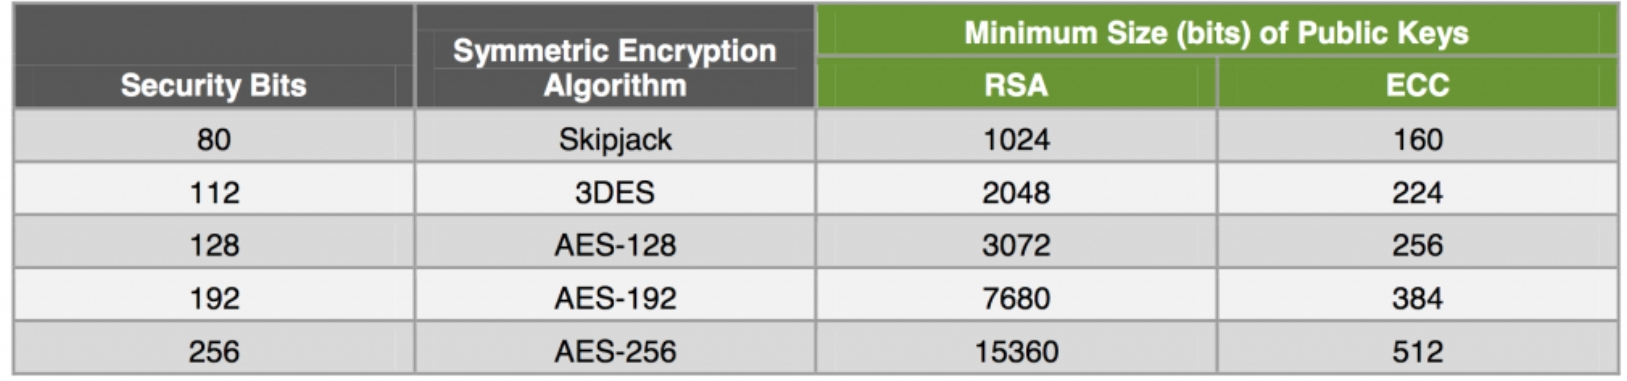
\includegraphics[width=0.8\textwidth]{image/section3/rsa.jpeg} 
    \caption[So sánh độ bảo mật giữa ECC và RSA]{So sánh độ bảo mật giữa ECC và RSA (\textbf{Nguồn:} \href{https://www.netburner.com/learn/comparing-rsa-and-ecc-encryption/}{NetBurner})}
    \label{}
\end{figure}

Có thể thấy rằng, mức bảo mật của khóa ECC-256 tương đương với khóa RSA-3072, trong khi kích thước khóa ECC nhỏ hơn hơn mười lần. Ưu điểm này mang lại lợi ích đáng kể trong các hệ thống nhúng (Embedded systems), nơi bộ nhớ, năng lượng và khả năng tính toán bị giới hạn.

\subsubsection{Đường cong NIST P-256}

Trong đề tài này, đường cong elliptic NIST P-256 (còn được gọi là \textit{secp256r1}) được sử dụng. Đường cong này được chuẩn hóa trong FIPS 186-4 \cite{fips186} và được xây dựng trên trường hữu hạn $\mathbb{F}_p$, với phương trình Weierstrass tổng quát:

\begin{equation}
y^2 \equiv x^3 + ax + b \pmod{p}
\end{equation}

\textbf{Các tham số của đường cong P-256} được xác định như sau:

\begin{align}
p &= 2^{256} - 2^{224} + 2^{192} + 2^{96} - 1 \\
a &= -3 \\
b &= \text{0x5AC635D8...} \quad \text{(hằng số 256 bit)}
\end{align}

Điểm sinh (base point) $G$ của đường cong có bậc (order) $n$ là một số nguyên tố lớn:

\begin{equation}
n = \text{0xFFFFFFFF00000000...} \quad \text{(số nguyên tố 256 bit)}
\end{equation}
\begin{figure}[H]
    \centering
    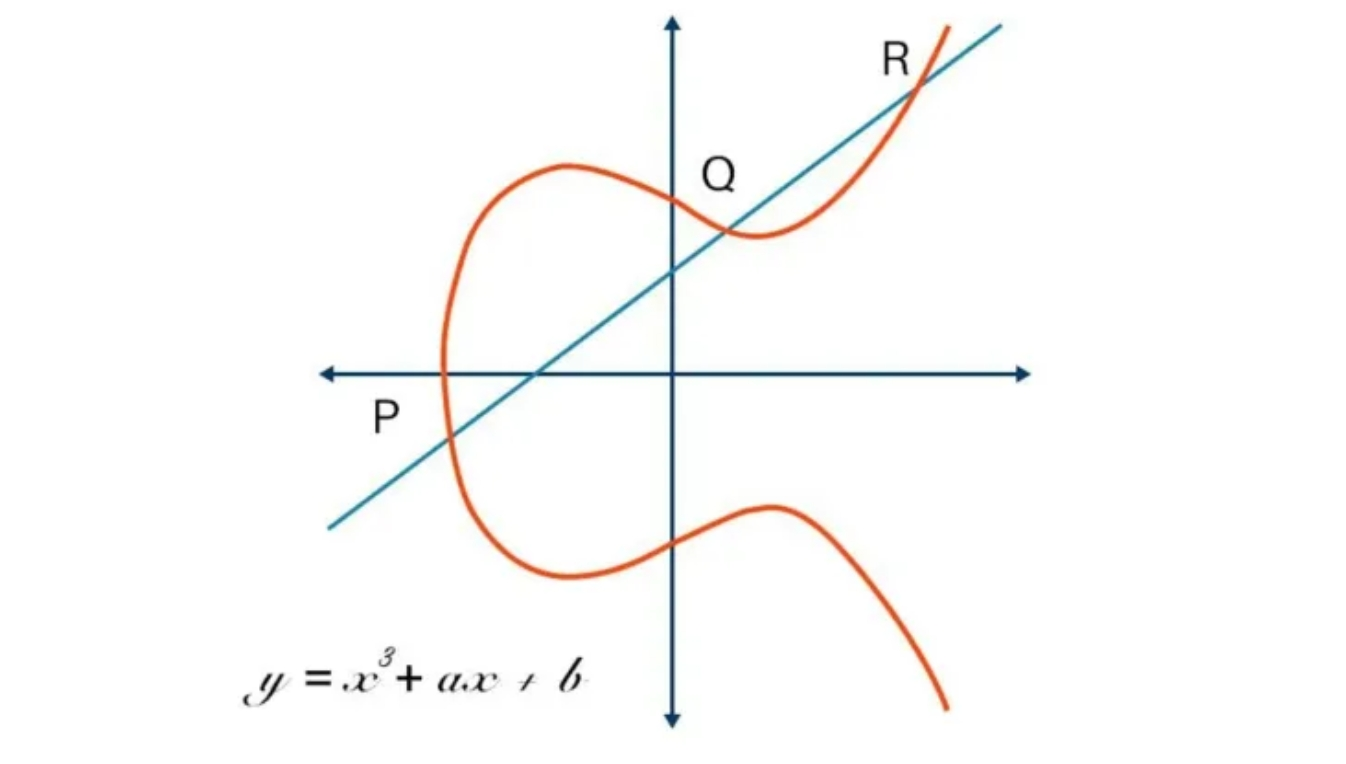
\includegraphics[width=0.8\textwidth]{image/section3/cry.jpeg} 
    \caption[Đồ thị đường cong Elliptic]{Đồ thị đường cong Elliptic (\textbf{Nguồn:} \href{https://blog.consultanubhav.com/elliptic-curve-cryptography-via-ope-5e91c059b817}{blog.consultanubhav.com})}
    \label{}
\end{figure}

\textbf{Các phép toán cơ bản trên đường cong}

\begin{itemize}
    \item \textbf{Cộng điểm (Point Addition):}  
    Cho hai điểm $P$ và $Q$ thuộc đường cong elliptic, phép cộng điểm tạo ra điểm thứ ba $R = P + Q$, được tính toán thông qua các phép toán đại số trên trường hữu hạn modulo $p$.
    
    \item \textbf{Nhân vô hướng (Scalar Multiplication):}  
    Phép nhân vô hướng là phép toán lặp phép cộng điểm nhiều lần:
    \begin{equation}
    Q = k \cdot P = \underbrace{P + P + \cdots + P}_{k \text{ lần}}
    \end{equation}
    Trong thực tế, phép toán này được thực hiện hiệu quả bằng thuật toán \textit{double-and-add}, với độ phức tạp tính toán là $O(\log k)$.
\end{itemize}

\textbf{Bài toán logarit rời rạc trên đường cong elliptic (ECDLP)}

Mức độ an toàn của ECC dựa trên độ khó của bài toán logarit rời rạc trên đường cong elliptic, được mô tả như sau:

\begin{quotation}
\textit{Cho hai điểm $P$ và $Q = k \cdot P$ trên đường cong elliptic, việc xác định giá trị vô hướng $k$ từ $P$ và $Q$ là một bài toán có độ phức tạp tính toán rất cao.}
\end{quotation}

Hiện nay, thuật toán hiệu quả nhất để giải bài toán ECDLP là thuật toán Pollard’s rho, với độ phức tạp xấp xỉ $O(\sqrt{n})$. Đối với đường cong P-256, độ phức tạp này tương đương khoảng $2^{128}$ phép toán, vượt quá khả năng tính toán của các hệ thống hiện tại.

\subsubsection{ECDH (Elliptic Curve Diffie-Hellman)}

ECDH (Elliptic Curve Diffie-Hellman) là giao thức trao đổi khóa dựa trên mật mã đường cong elliptic, cho phép hai bên thiết lập một \textbf{khóa bí mật chung} (shared secret) thông qua một kênh truyền không bảo mật. Giao thức này được chuẩn hóa trong NIST SP 800-56A Rev. 3 \cite{nist80056a} và được sử dụng rộng rãi trong các hệ thống bảo mật hiện đại.

\begin{figure}[htbp]
    \centering
    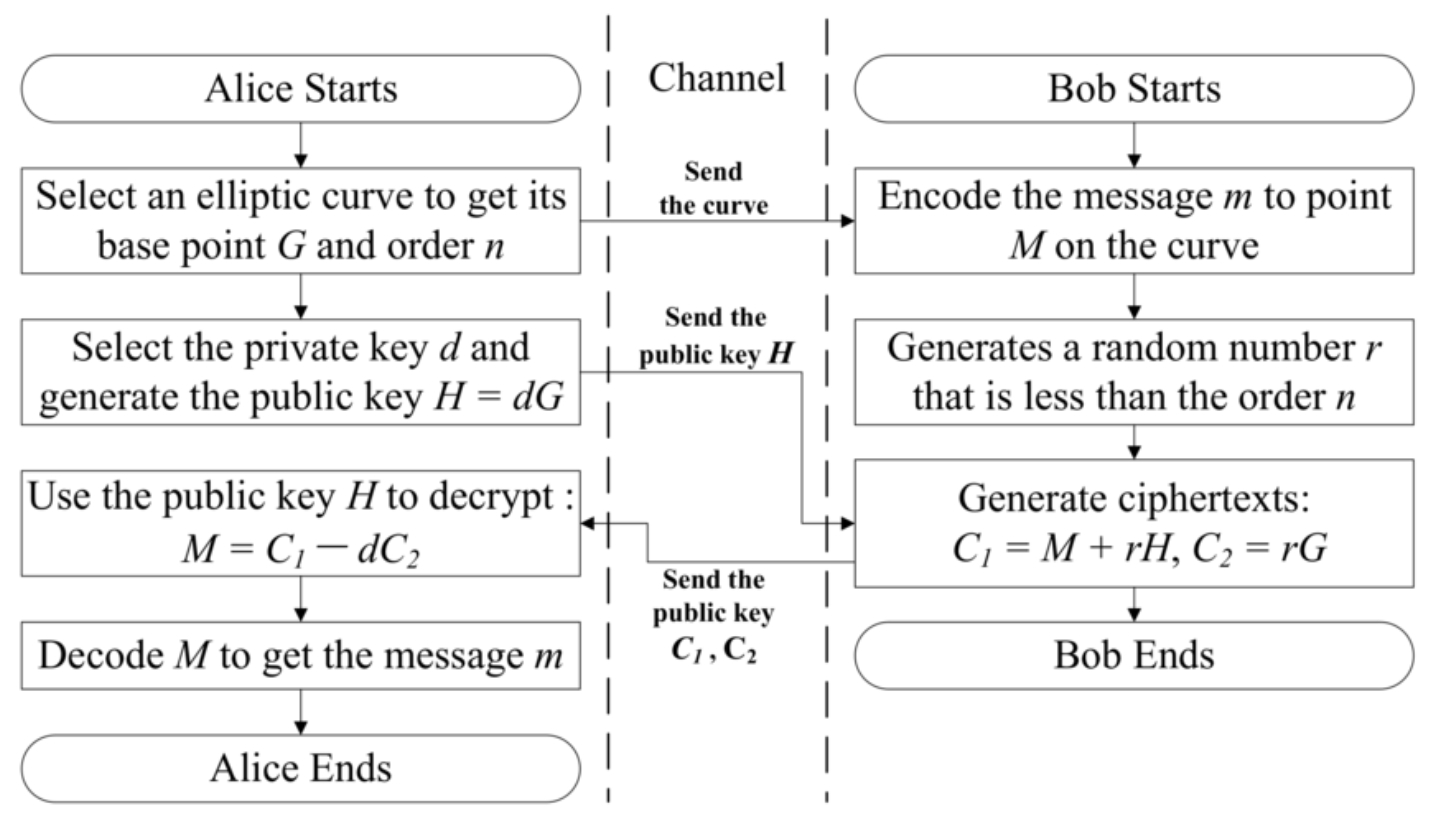
\includegraphics[width=0.8\textwidth]{image/section3/cry2.jpeg} 
    \caption[Sơ đồ giao thức ECDH]{Sơ đồ giao thức ECDH (\textbf{Nguồn:} \href{https://www.mdpi.com/2079-9292/11/18/2925}{MDPI})}
    \label{}
\end{figure}

\textbf{Quy trình giao thức ECDH}

Giả sử hai thực thể tham gia giao tiếp là Alice và Bob, quá trình thiết lập khóa được thực hiện như sau:

\begin{enumerate}
    \item \textbf{Alice tạo cặp khóa:}
    \begin{itemize}
        \item Khóa riêng: $d_A \in [1, n-1]$, được sinh ngẫu nhiên
        \item Khóa công khai: $Q_A = d_A \cdot G$
    \end{itemize}
    
    \item \textbf{Bob tạo cặp khóa:}
    \begin{itemize}
        \item Khóa riêng: $d_B \in [1, n-1]$, được sinh ngẫu nhiên
        \item Khóa công khai: $Q_B = d_B \cdot G$
    \end{itemize}
    
    \item \textbf{Trao đổi khóa công khai:}  
    Alice gửi khóa công khai $Q_A$ cho Bob; Bob gửi khóa công khai $Q_B$ cho Alice thông qua kênh truyền không bảo mật.
    
    \item \textbf{Tính toán khóa bí mật chung:}
    \begin{itemize}
        \item Alice tính:
        \[
        S = d_A \cdot Q_B = d_A \cdot (d_B \cdot G)
        \]
        \item Bob tính:
        \[
        S = d_B \cdot Q_A = d_B \cdot (d_A \cdot G)
        \]
    \end{itemize}
\end{enumerate}

Nhờ tính giao hoán của phép nhân vô hướng trên đường cong elliptic, cả hai bên thu được cùng một khóa bí mật chung:
\[
S = (d_A \cdot d_B) \cdot G
\]

\textbf{Các tính chất bảo mật}

\begin{itemize}
    \item \textbf{Tính bảo mật:}  
    Kẻ tấn công có thể quan sát được các khóa công khai $Q_A$ và $Q_B$, nhưng không thể suy ra khóa bí mật chung $S$ nếu không biết khóa riêng $d_A$ hoặc $d_B$. Điều này dựa trên độ khó của bài toán logarit rời rạc trên đường cong elliptic (ECDLP).
    
    \item \textbf{Forward Secrecy:}  
    Khi sử dụng \textbf{ephemeral keys} (cặp khóa tạm thời được tạo mới cho mỗi phiên), việc lộ khóa dài hạn không ảnh hưởng đến các khóa phiên đã được thiết lập trước đó.
\end{itemize}

\textbf{Ứng dụng trong đề tài}
\par\vspace{0.5em}
Trong đề tài này, ECDH được sử dụng ở \textbf{Phase B} của quá trình xác thực. Hai bên tạo cặp khóa ECDH tạm thời để thiết lập shared secret, sau đó sử dụng hàm dẫn xuất khóa HKDF để sinh ra các khóa phiên phục vụ cho mã hóa dữ liệu và kiểm tra toàn vẹn thông điệp (MAC).

\subsubsection{ECDSA (Elliptic Curve Digital Signature Algorithm)}

ECDSA (Elliptic Curve Digital Signature Algorithm) là thuật toán chữ ký số dựa trên mật mã đường cong elliptic (ECC), được chuẩn hóa trong tiêu chuẩn FIPS 186-4 \cite{fips186}. Thuật toán này cung cấp hai thuộc tính bảo mật quan trọng là \textbf{xác thực danh tính} (Authentication) và \textbf{tính không thể chối bỏ} (Non-repudiation).
\par\vspace{0.5em}
\textbf{Quy trình tạo chữ ký (Signing)}

Để tạo chữ ký số cho thông điệp $m$ bằng khóa riêng $d$, các bước được thực hiện như sau:

\begin{enumerate}
    \item Tính giá trị băm của thông điệp:
    \[
    e = \text{SHA-256}(m) \bmod n
    \]
    
    \item Sinh một số ngẫu nhiên bí mật (nonce):
    \[
    k \in [1, n-1]
    \]
    
    \item Tính điểm trên đường cong:
    \[
    R = k \cdot G = (x_R, y_R)
    \]
    
    \item Tính thành phần chữ ký thứ nhất:
    \[
    r = x_R \bmod n
    \]
    
    \item Tính thành phần chữ ký thứ hai:
    \[
    s = k^{-1} \cdot (e + r \cdot d) \bmod n
    \]
    
    \item Cặp giá trị $(r, s)$ tạo thành chữ ký số của thông điệp $m$.
\end{enumerate}

\textbf{Quy trình xác thực chữ ký (Verification)}

Để xác thực chữ ký $(r, s)$ của thông điệp $m$ bằng khóa công khai $Q$, các bước sau được thực hiện:

\begin{enumerate}
    \item Tính giá trị băm của thông điệp:
    \[
    e = \text{SHA-256}(m) \bmod n
    \]
    
    \item Tính nghịch đảo modulo của $s$:
    \[
    w = s^{-1} \bmod n
    \]
    
    \item Tính các hệ số trung gian:
    \[
    u_1 = e \cdot w \bmod n, \quad
    u_2 = r \cdot w \bmod n
    \]
    
    \item Tính điểm trên đường cong:
    \[
    P = u_1 \cdot G + u_2 \cdot Q = (x_P, y_P)
    \]
    
    \item Chữ ký được chấp nhận nếu:
    \[
    r \equiv x_P \bmod n
    \]
\end{enumerate}

\textbf{Các lưu ý bảo mật quan trọng}

\begin{itemize}
    \item \textbf{Tái sử dụng nonce:}  
    Việc sử dụng lại cùng một nonce $k$ cho nhiều chữ ký khác nhau là cực kỳ nguy hiểm, vì kẻ tấn công có thể khai thác để khôi phục khóa riêng $d$.
    
    \item \textbf{Bộ sinh số ngẫu nhiên:}  
    Nonce $k$ phải được sinh bằng bộ sinh số ngẫu nhiên an toàn về mặt mật mã (Cryptographically secure RNG) nhằm đảm bảo tính không thể dự đoán.
\end{itemize}

\textbf{Ứng dụng trong đề tài}
\par\vspace{0.5em}
ECDSA được sử dụng xuyên suốt trong hệ thống để đảm bảo xác thực danh tính và tính toàn vẹn dữ liệu:

\begin{itemize}
    \item \textbf{Phase A:} Điện thoại ký khóa công khai bằng khóa riêng định danh (identity private key), ESP32 xác thực chữ ký bằng khóa công khai đã được lưu trữ trước đó.
    
    \item \textbf{Phase B:} Điện thoại ký khóa công khai tạm thời (Ephemeral public key) và thông điệp thử thách (Challenge) nhằm chứng minh danh tính.
    
    \item Thư viện \textbf{mbedTLS} được sử dụng để triển khai ECDSA, đảm bảo  các phép toán mật mã được thực hiện an toàn.
\end{itemize}

%-----------------------------------------------------------------------

\subsection{Mã hóa đối xứng và xác thực thông điệp}

\subsubsection{AES-128-GCM – Advanced Encryption Standard}

AES là thuật toán mã hóa đối xứng được NIST lựa chọn làm chuẩn vào năm 2001 \cite{daemen2002design}.  
GCM là một chế độ mã hóa xác thực, kết hợp đồng thời chức năng mã hóa và xác thực thông điệp trong cùng một phép toán, được chuẩn hóa trong NIST SP 800-38D \cite{nist80038d}.
\begin{figure}[htbp]
    \centering
    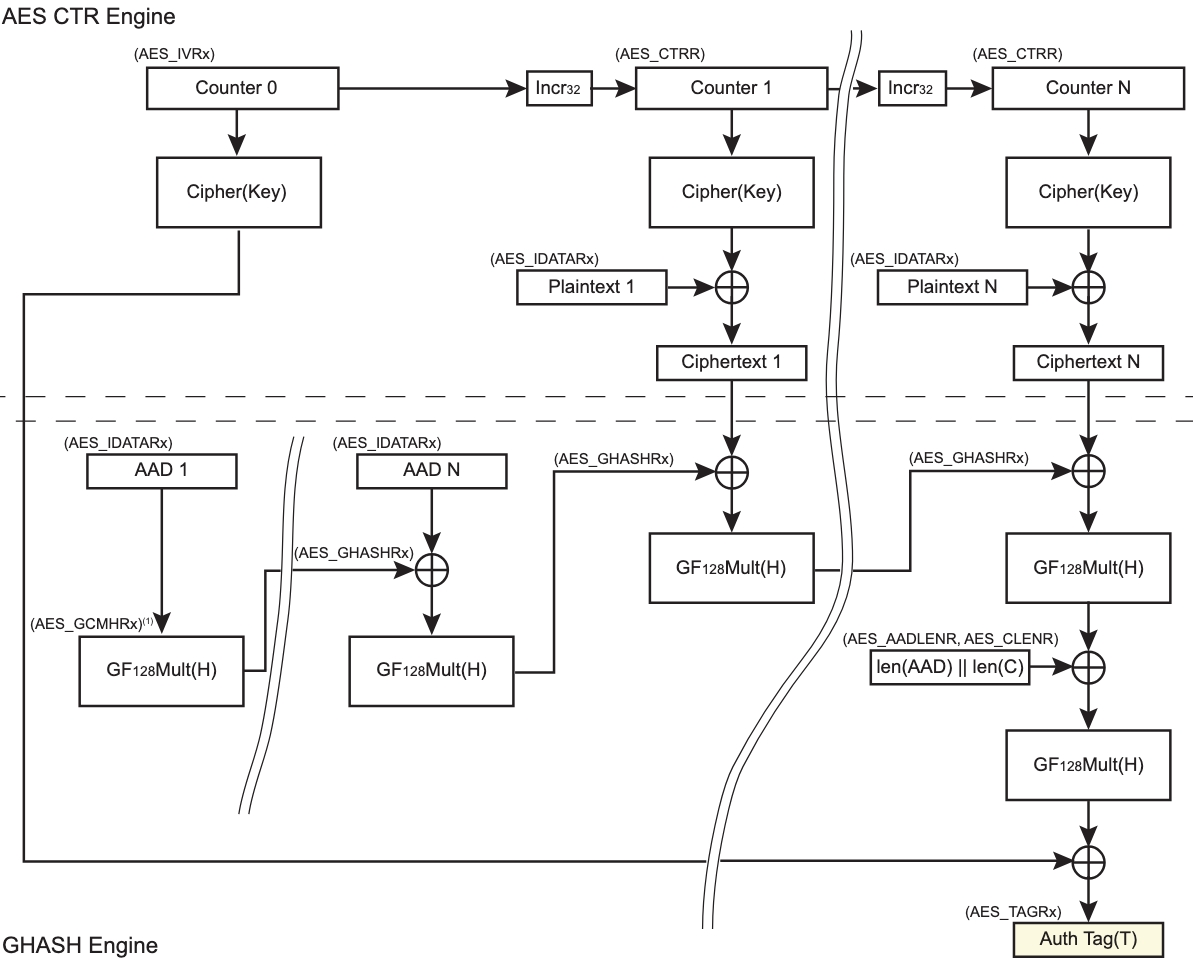
\includegraphics[width=0.8\textwidth]{image/section3/cry3.jpeg} 
    \caption[Cấu trúc AES-GCM]{Cấu trúc AES-GCM (\textbf{Nguồn:} \href{https://dl.acm.org/doi/10.1145/3766074}{dl.acm.org})}
    \label{}
\end{figure}

\textbf{Thông số kỹ thuật}

\begin{itemize}
    \item \textbf{Kích thước khóa:} 128 bit, đề tài sử dụng AES-128
    \item \textbf{Kích thước khối:} 128 bit
    \item \textbf{IV – Initialization Vector:} 96 bit, theo khuyến nghị của NIST
    \item \textbf{Authentication Tag:} 128 bit
\end{itemize}

\textbf{Thành phần của GCM}

\begin{enumerate}
    \item \textbf{Mã hóa theo chế độ CTR}

    Plaintext được XOR với keystream sinh ra từ quá trình mã hóa AES của giá trị counter:
    \begin{equation}
        C_i = P_i \oplus \text{AES}_K(\text{IV} \parallel \text{Counter}_i)
    \end{equation}

    \item \textbf{Xác thực bằng GHASH}

    Thuật toán GHASH sử dụng phép nhân trên trường Galois để tính toán authentication tag từ ciphertext và dữ liệu xác thực bổ sung:
    \begin{equation}
        T = \text{GHASH}_H(\text{AAD}, C)
    \end{equation}
\end{enumerate}

\textbf{Dữ liệu vào và dữ liệu ra}

\begin{itemize}
    \item \textbf{Dữ liệu vào:} Khóa $K$ 128 bit, IV 96 bit, Plaintext $P$, AAD (tùy chọn)
    \item \textbf{Dữ liệu ra:} Ciphertext $C$ và authentication tag $T$ 128 bit
\end{itemize}

\textbf{Các tính chất bảo mật}

\begin{itemize}
    \item \textbf{Confidentiality – Bảo mật:} Plaintext không thể được khôi phục nếu không có khóa bí mật
    \item \textbf{Authenticity – Xác thực:} Authentication tag cho phép phát hiện ciphertext bị giả mạo
    \item \textbf{Integrity – Toàn vẹn:} Bất kỳ thay đổi nào trong dữ liệu đều làm cho tag không hợp lệ
\end{itemize}

\textbf{Yêu cầu quan trọng}

\begin{itemize}
    \item \textbf{Tính duy nhất của IV:} IV phải là duy nhất cho mỗi lần mã hóa với cùng một khóa. Việc tái sử dụng IV gây ra lỗ hổng bảo mật nghiêm trọng \cite{joux2006authentication}.
    \item \textbf{Xác minh Authentication tag:} Authentication tag phải được kiểm tra trước khi sử dụng dữ liệu đã giải mã.
\end{itemize}

\textbf{Ứng dụng trong đề tài}
\par\vspace{0.5em}
Sau khi quá trình xác thực hoàn tất, AES-128-GCM được sử dụng để mã hóa dữ liệu trong phiên làm việc. IV(Initialization Vector) được sinh từ bộ sinh số ngẫu nhiên an toàn và kết hợp với Counter để đảm bảo tính duy nhất cho mỗi lần mã hóa.

\subsubsection{HMAC-SHA256 – Hash-based Message Authentication SHA-256}

HMAC là một cơ chế tạo mã xác thực thông điệp dựa trên hàm băm mật mã, được định nghĩa trong RFC 2104 \cite{rfc2104} và tiêu chuẩn hóa trong FIPS 198-1 \cite{fips198}.  
Thuật toán này kết hợp khóa bí mật với hàm băm để đảm bảo tính toàn vẹn và xác thực của dữ liệu trao đổi.
\par\vspace{0.5em}
\textbf{Công thức HMAC}

\begin{equation}
\text{HMAC}_K(m) = H\bigl((K \oplus \text{opad}) \parallel H((K \oplus \text{ipad}) \parallel m)\bigr)
\end{equation}

Trong đó:

\begin{itemize}
    \item $H$: Hàm băm mật mã, trong đề tài sử dụng SHA-256
    \item $K$: Khóa bí mật, độ dài 32 byte
    \item $\text{opad}$: Outer padding, giá trị 0x5c lặp lại theo độ dài khối
    \item $\text{ipad}$: Inner padding, giá trị 0x36 lặp lại theo độ dài khối
    \item $\parallel$: Phép nối chuỗi
\end{itemize}

\begin{figure}[H]
    \centering
    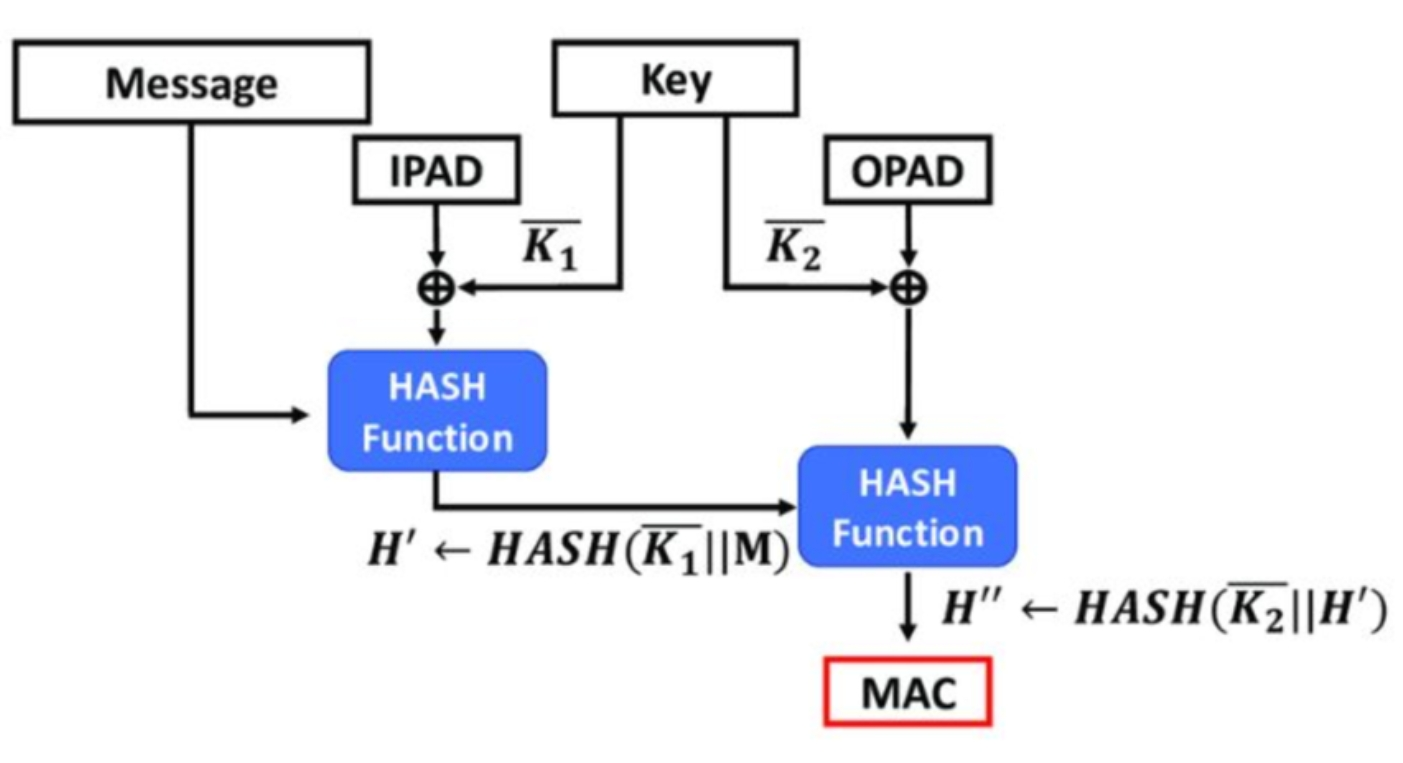
\includegraphics[width=0.8\textwidth]{image/section3/cry4.jpeg} 
    \caption[Cấu trúc HMAC]{Cấu trúc HMAC (\textbf{Nguồn:} \href{https://www.mdpi.com/2079-9292/9/11/1839}{MDPI})}
    \label{}
\end{figure}

\textbf{Thông số HMAC-SHA256 trong đề tài}

\begin{itemize}
    \item \textbf{Khóa đầu vào:} 32 byte, tương đương 256 bit
    \item \textbf{Giá trị đầu ra:} 32 byte, tương đương 256 bit
    \item \textbf{Mức độ bảo mật:} $2^{128}$, xét theo khả năng chống tấn công preimage đối với output rút gọn
\end{itemize}

\textbf{Các tính chất bảo mật}

\begin{itemize}
    \item \textbf{Unforgeability – Không thể giả mạo:} Không thể tạo ra HMAC hợp lệ nếu không biết khóa bí mật
    \item \textbf{Collision resistance – Chống va chạm:} Khó tìm hai thông điệp khác nhau cho cùng một giá trị HMAC
    \item \textbf{Key recovery resistance – Chống phục hồi khóa:} Không thể suy ra khóa bí mật từ các giá trị HMAC quan sát được
\end{itemize}

\textbf{Ứng dụng trong đề tài}

\begin{itemize}
    \item \textbf{Xác thực hai chiều:}  
    Điện thoại gửi $\text{HMAC}_{K_{c2s}}$ (Client confirm), thiết bị ESP32 xác minh và phản hồi bằng $\text{HMAC}_{K_{s2c}}$ (Server confirm)
    
    \item \textbf{Dẫn xuất khóa:}  
    Thuật toán HKDF sử dụng HMAC-SHA256 làm Primitive mật mã để sinh các Session keys
\end{itemize}


\subsubsection{HKDF – Hàm dẫn xuất khóa dựa trên HMAC}

HKDF là một hàm dẫn xuất khóa dựa trên HMAC, được định nghĩa trong RFC 5869 \cite{rfc5869}.  
Thuật toán này cho phép sinh ra nhiều khóa mật mã độc lập từ một Shared secret ban đầu, thường thu được từ các giao thức trao đổi khóa như ECDH.

\textbf{Cấu trúc của HKDF}

HKDF gồm hai giai đoạn liên tiếp: trích xuất và mở rộng.

\begin{enumerate}
    \item \textbf{Giai đoạn trích xuất – Extract Phase}
    
    Giai đoạn này chuyển Input keying material thành một khóa giả ngẫu nhiên có tính Entropy cao hơn, gọi là Pseudorandom key (PRK):
    \begin{equation}
    \text{PRK} = \text{HMAC}(\text{salt}, \text{IKM})
    \end{equation}
        \begin{figure}[H]
        \centering
        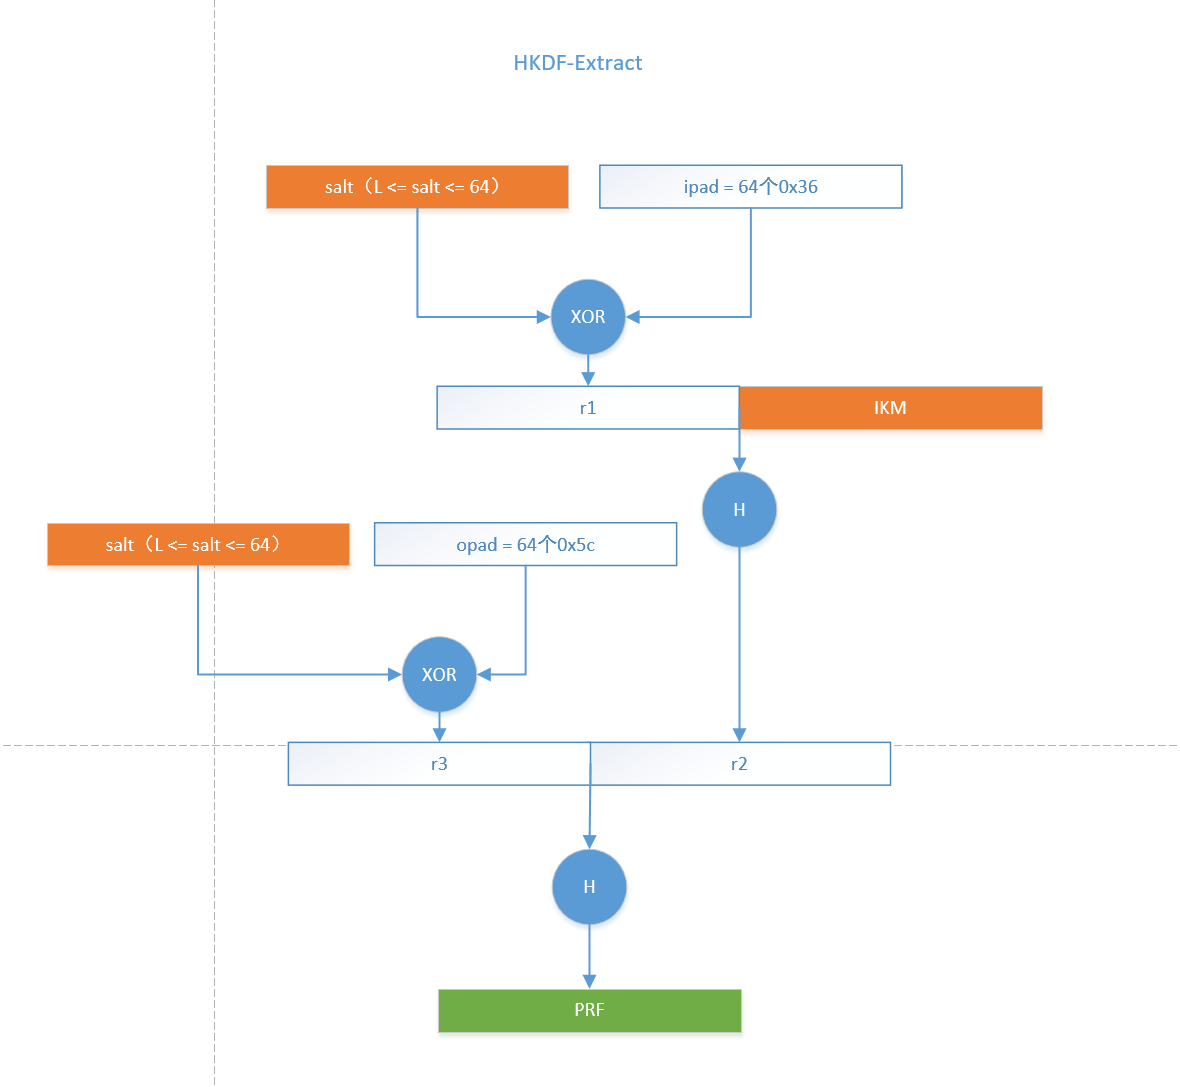
\includegraphics[width=0.5\textwidth]{image/section3/cry6.png} 
        \caption[Cấu trúc HKDF Extract]{Cấu trúc HKDF Extract (\textbf{Nguồn:} \href{https://suntus.github.io/2019/05/09/HKDF\%E7\%AE\%97\%E6\%B3\%95/}{HKDF - Morning~Sun})}
        \label{fig: hkdf_extract}
        \end{figure}
    \item \textbf{Giai đoạn mở rộng – Expand Phase}
    
    PRK được sử dụng để sinh ra một hoặc nhiều khóa đầu ra thông qua thông tin ngữ cảnh:
    \begin{align}
    T(0) &= \text{chuỗi rỗng} \\
    T(i) &= \text{HMAC}(\text{PRK}, T(i-1) \parallel \text{info} \parallel i)
    \end{align}
\end{enumerate}

\begin{figure}[H]
    \centering
    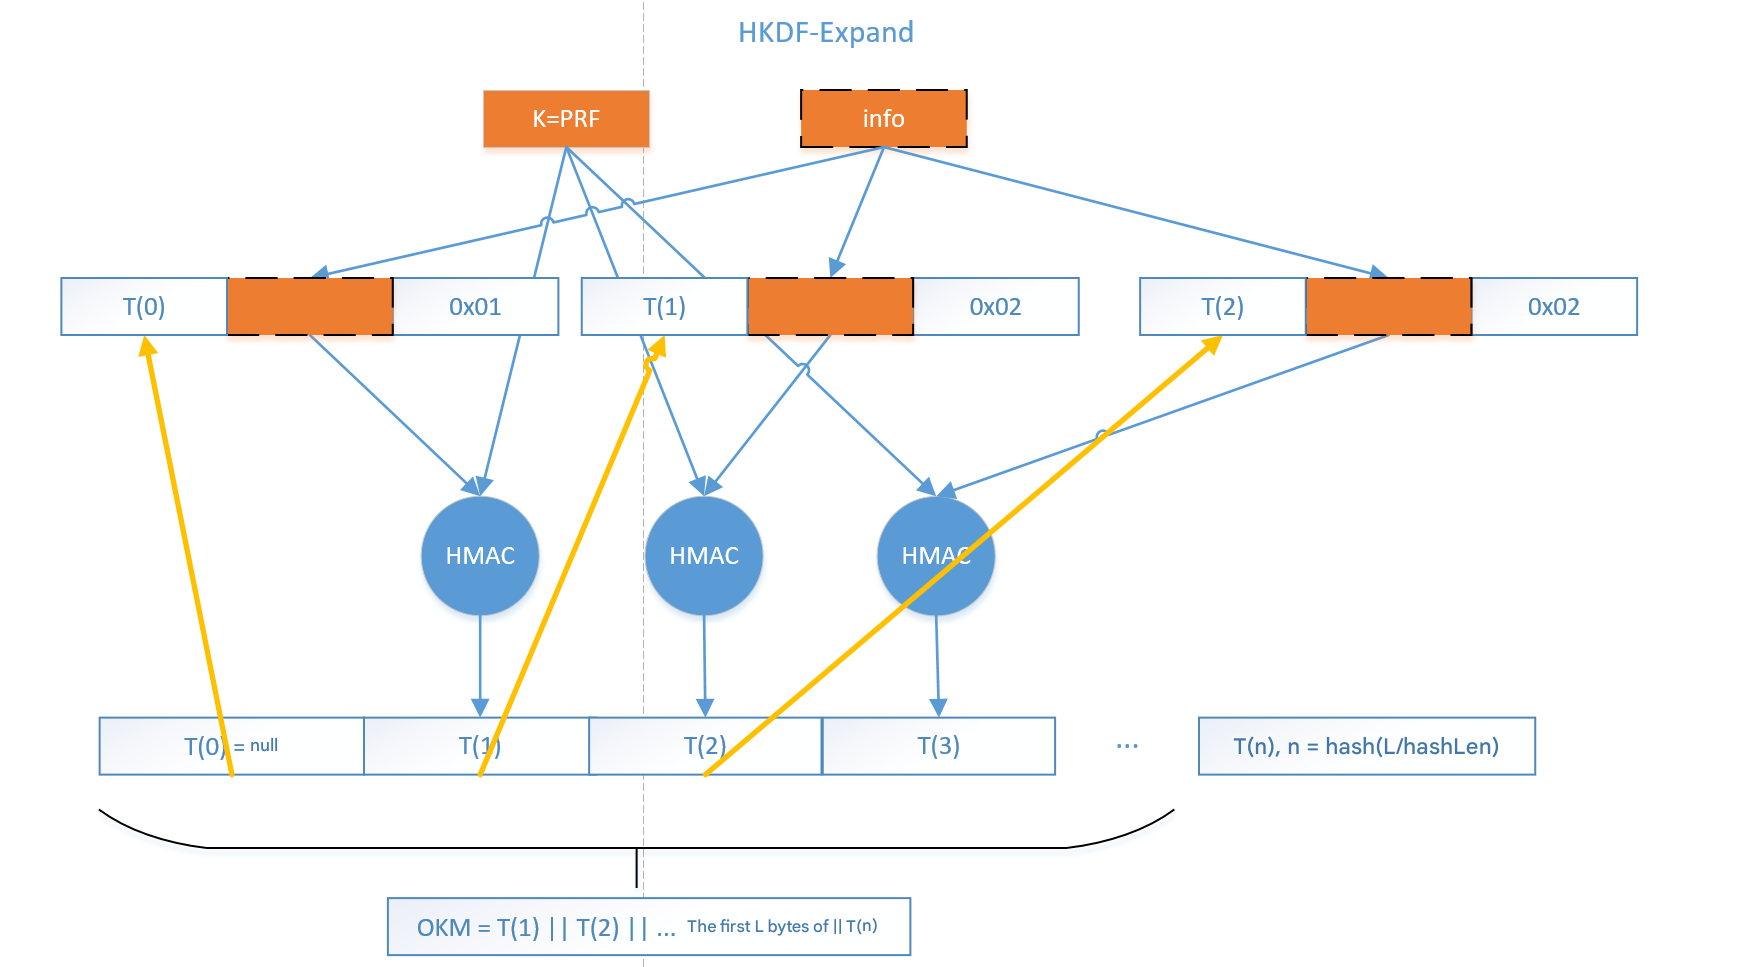
\includegraphics[width=0.8\textwidth]{image/section3/cry7.png} 
    \caption[Cấu trúc HKDF Expand]{Cấu trúc HKDF Expand (\textbf{Nguồn:} \href{https://suntus.github.io/2019/05/09/HKDF\%E7\%AE\%97\%E6\%B3\%95/}{HKDF - Morning~Sun})}
    \label{fig: hkdf_expand}
\end{figure}

\textbf{Các tham số của HKDF}

\begin{itemize}
    \item \textbf{IKM – Input Keying Material:} Dữ liệu đầu vào cho HKDF, trong đề tài là shared secret thu được từ ECDH, độ dài 32 byte
    \item \textbf{Salt:} Giá trị ngẫu nhiên tùy chọn dùng trong giai đoạn extract, không được sử dụng trong đề tài
    \item \textbf{Info:} Thông tin ngữ cảnh để ràng buộc khóa với phiên và ứng dụng cụ thể
    \item \textbf{L:} Độ dài khóa đầu ra mong muốn
\end{itemize}

\textbf{Tính chất bảo mật}

\begin{itemize}
    \item \textbf{Key independence – Tính độc lập của khóa:}  
    Các khóa được dẫn xuất với giá trị Info khác nhau là độc lập về mặt mật mã
    
    \item \textbf{Forward compatibility – Khả năng mở rộng về sau:}  
    Có thể sinh thêm các khóa mới mà không ảnh hưởng đến các khóa đã tồn tại
\end{itemize}

\textbf{Ứng dụng trong đề tài}

Từ Shared secret thu được trong quá trình trao đổi khóa ECDH, đề tài dẫn xuất các khóa phiên (Session Keys) nhằm mã hóa kênh truyền BLE và liên kết trực tiếp với phiên đo khoảng cách UWB:

\begin{lstlisting}[language=C++]
       // 1. Encryption Key
       info_enc = "SmartCarv1|ENC" || ecuPubKey || phonePubKey
       K_enc = HKDF-SHA256(sharedSecret, salt="", info_enc, L=32)

       // 2. MAC Key
       info_mac = "SmartCarv1|MAC" || ecuPubKey || phonePubKey
       K_mac = HKDF-SHA256(sharedSecret, salt="", info_mac, L=32)
       
       // 3. URSK - UWB Ranging Session Key
       info_uwb = "SmartCarv1|URSK" || ecuPubKey || phonePubKey
       K_ursk = HKDF-SHA256(sharedSecret, salt="", info_uwb, L=32)
\end{lstlisting}

Điểm đột phá trong giao thức bảo mật của đề tài (bám sát CCC Release 3) là việc khóa \texttt{K\_ursk} được sinh ra từ chính phiên giao tiếp BLE. Khóa này sau đó được nạp vào vi mạch UWB để mã hóa chuỗi STS (Scrambled Timestamp Sequence). Sự ràng buộc mật mã này đảm bảo rằng: Ngay cả khi kẻ tấn công can thiệp được vào sóng UWB, chúng cũng không thể giải mã hoặc đánh lừa được hệ thống đo khoảng cách vì không sở hữu khóa phiên bắt nguồn từ giao dịch BLE.
%-----------------------------------------------------------------------

\subsection{Tuân thủ chuẩn quốc tế}

Giao thức bảo mật của đề tài được thiết kế tuân thủ các chuẩn sau:

\begin{table}[h]
\centering
\label{tab:crypto_standards}
\begin{tabular}{|l|l|p{6cm}|}
\hline
\textbf{Chuẩn} & \textbf{Thuật toán} & \textbf{Mô tả} \\
\hline
NIST SP 800-56A Rev. 3 & ECDH & Key agreement với P-256 curve \\
\hline
FIPS 186-4 & ECDSA & Digital signature với P-256 \\
\hline
NIST SP 800-38D & AES-GCM & Authenticated encryption \\
\hline
FIPS 198-1 & HMAC-SHA256 & Message authentication \\
\hline
RFC 5869 & HKDF & Key derivation function \\
\hline
ISO/IEC 7816-4 & APDU & NFC communication protocol \\
\hline
\end{tabular}
\caption{Chuẩn mật mã được áp dụng}
\end{table}

Việc tuân thủ các chuẩn quốc tế đảm bảo:
\begin{itemize}
    \item Tính tương thích (Interoperability)
    \item Độ tin cậy về bảo mật (Security assurance)
    \item Khả năng chấp nhận trong công nghiệp (Industry acceptance)
\end{itemize}


\section{Công nghệ phát triển ứng dụng di động}

Ứng dụng di động (Smart Car) trong hệ thống được phát triển dựa trên Flutter Framework kết hợp với hệ sinh thái Firebase. Trong kiến trúc Hybrid Cloud của đề tài, Flutter không chỉ đảm nhiệm việc xây dựng giao diện người dùng mà còn đóng vai trò là Gateway trung gian, quản lý máy trạng thái (FSM) của khóa kỹ thuật số theo chuẩn CCC, xử lý các luồng dữ liệu bất đồng bộ từ phần cứng (BLE, UWB, NFC) và đồng bộ hóa với dịch vụ Cloud.

\subsection{Flutter Framework và Quản lý trạng thái}

Flutter là framework mã nguồn mở do Google phát triển, cho phép xây dựng ứng dụng đa nền tảng từ một codebase duy nhất sử dụng ngôn ngữ Dart. Đặc trưng nổi bật của Flutter là cơ chế biên dịch Ahead-of-Time (AOT), chuyển mã Dart trực tiếp sang mã máy ARM hoặc x86. Thay vì sử dụng JavaScript bridge hoặc WebView như các framework hybrid truyền thống, Flutter tự render toàn bộ giao diện thông qua đồ họa Skia/Impeller, giúp ứng dụng đạt hiệu năng cao và thời gian phản hồi thấp, đáp ứng tốt yêu cầu xử lý thời gian thực của hệ thống Smart Key.

\begin{figure}[H]
    \centering
    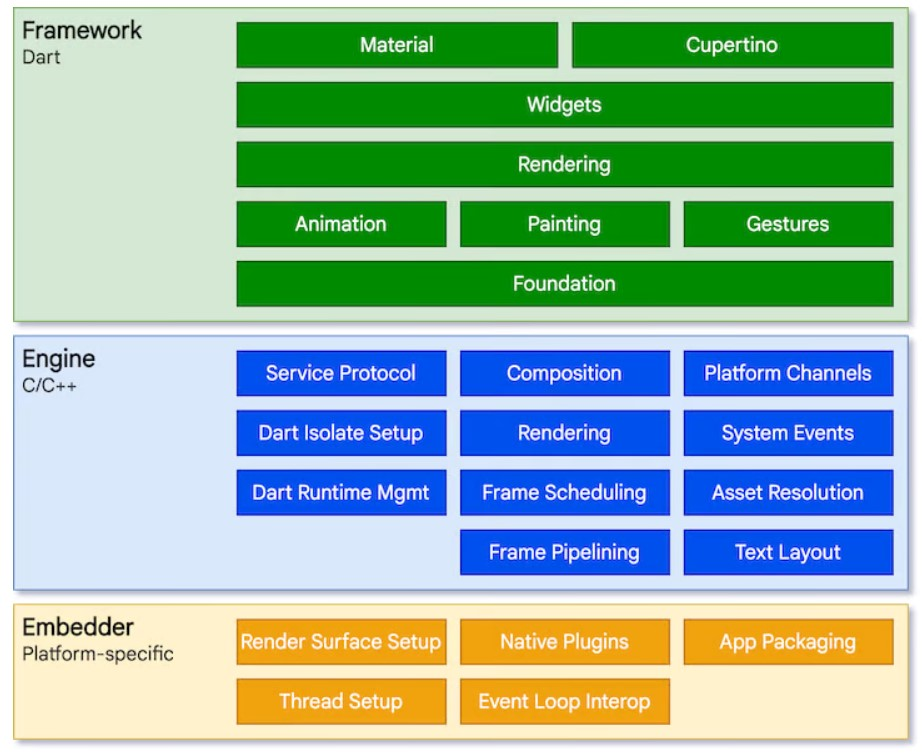
\includegraphics[width=0.8\textwidth]{image/section3/flu.jpg}
    \caption[Kiến trúc tổng thể của Flutter Framework]{Kiến trúc tổng thể của Flutter Framework (\textbf{Nguồn:} \href{https://bizflycloud.vn/tin-tuc/flutter-la-gi-tim-hieu-tinh-nang-noi-troi-cua-nen-tang-lap-trinh-flutter-20220623155918472.htm}{BizFlyCloud})}
    \label{fig: flutter_architecture}
\end{figure}

Kiến trúc của Flutter được tổ chức thành bốn tầng chính, hỗ trợ đắc lực cho việc phát triển ứng dụng giao tiếp phần cứng sâu:
\begin{itemize}
    \item \textbf{Application Layer:} Chứa mã Dart do lập trình viên xây dựng. Để quản lý sự phức tạp của các sự kiện phần cứng và luồng xác thực đa bước, ứng dụng áp dụng kiến trúc \textbf{BLoC (Business Logic Component)}. Mô hình này tách biệt hoàn toàn giao diện (UI) khỏi logic nghiệp vụ, giúp xử lý mượt mà các luồng dữ liệu (Streams) liên tục từ BLE, UWB và Firebase.
    \item \textbf{Framework Layer:} Cung cấp hệ thống widget nền tảng (Material, Cupertino), quản lý animation và pipeline render giao diện.
    \item \textbf{Engine Layer:} Core engine viết bằng C++, bao gồm đồ họa, Dart runtime và quản lý luồng (thread management).
    \item \textbf{Embedder Layer:} Đóng vai trò cầu nối giữa Flutter engine và hệ điều hành cụ thể (Android/iOS).
\end{itemize}

\textbf{Tương tác phần cứng qua Platform Channels:} \\
Một trong những lý do cốt lõi để chọn Flutter cho đề tài này là cơ chế Platform Channels. Cơ chế này cho phép luồng mã Dart giao tiếp trực tiếp và hai chiều với mã Native (Java/Kotlin trên Android, Swift trên iOS) thông qua \textit{MethodChannel} và \textit{EventChannel}. 

Tính năng này mang tính quyết định trong việc hiện thực hóa các chức năng bậc cao của chuẩn CCC Release 3, bao gồm:
\begin{itemize}
    \item Giao tiếp trực tiếp với các API Native của hệ điều hành để cấu hình \textbf{phiên UWB (UWB Session)} phục vụ đo khoảng cách an toàn (Secure Ranging).
    \item Thiết lập và duy trì \textbf{Background Services} cho phép ứng dụng quét BLE ngầm, phục vụ tính năng Auto-Unlock (Fast Authentication) mà không cần mở ứng dụng.
    \item Kích hoạt chế độ mô phỏng thẻ \textbf{NFC HCE (Host Card Emulation)}, biến điện thoại thành thẻ từ để thực hiện giao dịch Phase 0 dự phòng.
\end{itemize}

\subsection{Firebase Backend-as-a-Service}
Firebase là nền tảng Backend-as-a-Service (BaaS) do Google cung cấp, bao gồm tập hợp các dịch vụ backend được quản lý sẵn như xác thực người dùng, cơ sở dữ liệu thời gian thực, lưu trữ và điện toán phi máy chủ (serverless) \cite{firebase_docs}. Nền tảng này cho phép ứng dụng client giao tiếp trực tiếp với backend thông qua các SDK tích hợp sẵn hoặc REST API, giúp giảm thiểu tối đa sự phức tạp trong việc triển khai, duy trì và mở rộng hệ thống máy chủ vật lý.
\begin{figure}[H]
    \centering
    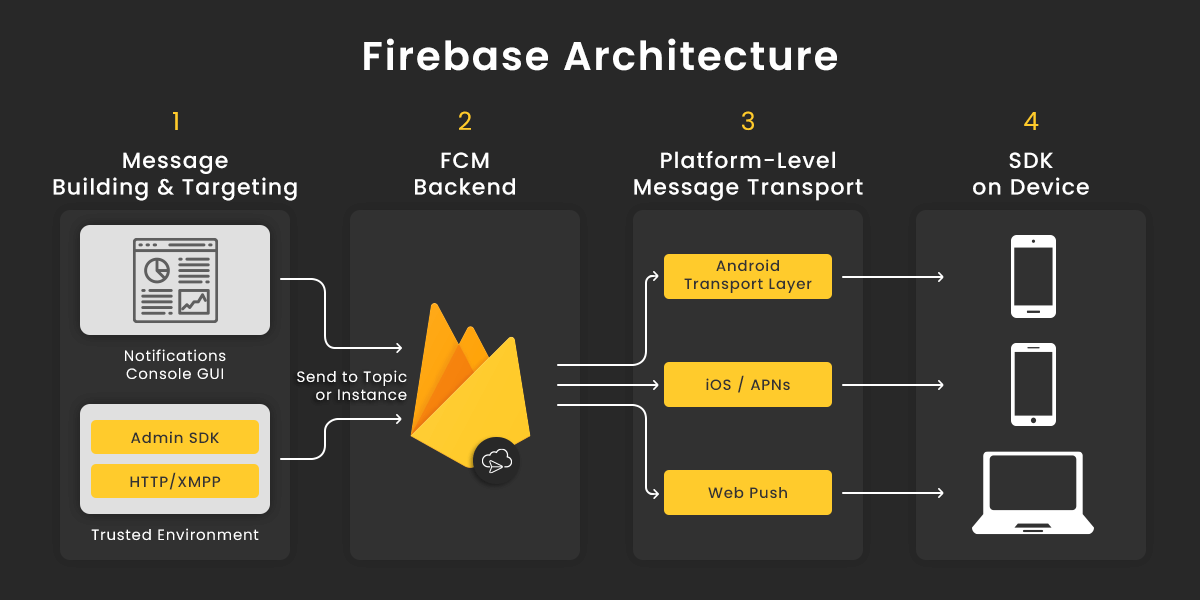
\includegraphics[width=0.85\textwidth]{image/section3/fire.png}
    \caption[Kiến trúc các dịch vụ Firebase trong hệ thống]{Kiến trúc các dịch vụ Firebase trong hệ thống (\textbf{Nguồn:} \href{https://bumblebeedev.hashnode.dev/2024-guide-to-creating-scalable-backend-apis-with-firebase}{BumblebeeDev})}
    \label{fig:firebase_architecture}
\end{figure}
\begin{itemize}
    \item \textbf{Firebase Authentication (Xác thực và định danh):}\\
    Trong hệ thống, Firebase Authentication được sử dụng để quản lý quá trình xác thực và định danh người dùng. Dịch vụ này hỗ trợ đa dạng các phương thức đăng nhập và tự động quản lý toàn bộ vòng đời của phiên làm việc (session), bao gồm việc phát hành, mã hóa và làm mới token (Token refresh). Firebase Authentication tuân thủ các tiêu chuẩn bảo mật mạng toàn cầu như OAuth 2.0 và OpenID Connect, đảm bảo an toàn tuyệt đối cho thông tin định danh trước các rủi ro đánh cắp phiên (Session Hijacking) hoặc nghe lén (Eavesdropping).

    \item \textbf{Cloud Firestore và Realtime Database (Lưu trữ và đồng bộ thời gian thực):}\\
    Cloud Firestore là cơ sở dữ liệu NoSQL dạng tài liệu (Document-based) của Firebase, được tối ưu hóa cho khả năng đồng bộ dữ liệu thời gian thực (Real-time synchronization) giữa các client. Dữ liệu được tổ chức theo mô hình phân cấp Collection và Document, cho phép linh hoạt lưu trữ các cấu trúc dữ liệu phức tạp. Cơ sở dữ liệu này hỗ trợ cơ chế cache dữ liệu ngoại tuyến (offline caching), tự động giải quyết xung đột và đồng bộ trạng thái khi kết nối mạng được khôi phục. 
    
    Bên cạnh đó, hệ thống phân quyền của Firestore được kiểm soát chặt chẽ thông qua Security Rules thực thi tại phía server. Cơ chế này đảm bảo chỉ những thiết bị hoặc người dùng có token hợp lệ, được cấp quyền tương ứng mới có thể thực hiện các thao tác truy xuất (Read) hoặc thay đổi (Write) dữ liệu, tạo ra một lớp phòng thủ độc lập hoàn toàn với client.

    \item \textbf{Firebase Cloud Messaging (FCM) - Giao thức truyền tin nhắn:}\\
    Firebase Cloud Messaging (FCM) là dịch vụ nhắn tin đa nền tảng, cung cấp cơ sở hạ tầng mạng định tuyến thông điệp có độ trễ thấp từ máy chủ đến thiết bị người dùng (Client). Trong các hệ thống yêu cầu tính thời gian thực cao, FCM đóng vai trò là kênh giao tiếp Push Notification tin cậy. Dịch vụ này sử dụng kiến trúc Pub/Sub (Publish/Subscribe), cho phép gửi cảnh báo ngay lập tức để đánh thức các ứng dụng đang chạy ngầm (background) hoặc đã tắt hoàn toàn (terminated), đảm bảo người dùng nhận được các thông báo an ninh quan trọng ngay tại thời điểm sự kiện phát sinh.

    \item \textbf{Khả năng tích hợp IoT và Event-Driven Architecture:}\\
    Mặc dù được thiết kế chủ yếu cho hệ sinh thái Web và Mobile, Firebase cung cấp hệ thống REST API mạnh mẽ, cho phép các thiết bị nhúng với tài nguyên phần cứng giới hạn (như vi điều khiển) giao tiếp trực tiếp qua giao thức HTTPS. Các thiết bị biên (Edge devices) có thể đẩy trực tiếp dữ liệu nhật ký hoạt động (Access Logs) hoặc trạng thái phần cứng lên cơ sở dữ liệu đám mây. 
    
    Khi kết hợp với \textbf{Firebase Cloud Functions} – môi trường thực thi mã backend phi máy chủ (Serverless), hệ thống có thể vận hành theo kiến trúc hướng sự kiện (Event-driven). Bất kỳ một luồng dữ liệu mới nào được ghi vào cơ sở dữ liệu từ thiết bị IoT cũng có thể trở thành một trigger (bộ kích hoạt), tự động gọi các hàm tính toán logic trên server hoặc giao tiếp với các hệ thống phân tích Trí tuệ nhân tạo (AI) bên thứ ba để phát hiện sự kiện bất thường mà không làm tiêu tốn tài nguyên của thiết bị biên.
\end{itemize}


Trong hệ thống, \textbf{Firebase Authentication} đảm nhiệm việc xác thực và định danh người dùng. Dịch vụ này tự động quản lý vòng đời phiên làm việc (cấp phát và làm mới token) dựa trên các tiêu chuẩn bảo mật nền tảng như OAuth 2.0 và OpenID Connect.

Bên cạnh đó, \textbf{Cloud Firestore} được sử dụng làm cơ sở dữ liệu NoSQL dạng tài liệu (document-based) nhằm lưu trữ linh hoạt và đồng bộ dữ liệu theo thời gian thực. Firestore hỗ trợ hoạt động ngoại tuyến (offline cache) và tích hợp cơ chế \textit{Security Rules} thực thi tại server, đảm bảo chỉ những client đã xác thực và có quyền hợp lệ mới được phép truy xuất hoặc thay đổi dữ liệu.




%----------------------------------------------------------------------------------------------



\section{Mô hình học sâu LSTM cho nhận diện hành vi}

Trong bài toán nhận diện hành vi người dùng dựa trên dữ liệu từ cảm biến UWB, các tín hiệu (khoảng cách, vận tốc, thặng dư) không tồn tại độc lập mà có sự phụ thuộc chặt chẽ vào thời gian. Các mạng nơ-ron truyền thống (Feed-forward Neural Network) không thể xử lý loại dữ liệu chuỗi này do thiếu cơ chế ghi nhớ các trạng thái quá khứ. Mạng nơ-ron hồi quy (RNN) ra đời để giải quyết vấn đề này, tuy nhiên RNN gặp phải hiện tượng "biến mất gradient" (Vanishing Gradient) khi xử lý các chuỗi dài, khiến mô hình không thể học được các phụ thuộc xa (long-term dependencies).Kiến trúc LSTM, được giới thiệu bởi Hochreiter \& Schmidhuber (1997), là một biến thể đặc biệt của RNN được thiết kế để khắc phục nhược điểm trên. Trong hệ thống Smart Car Access của đề tài, LSTM đóng vai trò nhận diện các "hình thái" chuyển động (như việc tiến lại gần xe hoặc các dao động bất thường của tấn công tiếp sóng) thông qua một cửa sổ thời gian (sliding window).

\subsection{Kiến trúc và cơ chế hoạt động của LSTM}Điểm khác biệt cốt lõi của LSTM là sự xuất hiện của Trạng thái tế bào (Cell State) — đóng vai trò như một "băng chuyền" thông tin chạy xuyên suốt chuỗi — và các Cổng (Gates) để điều tiết việc thêm hoặc bớt thông tin vào trạng thái đó.Mỗi tế bào LSTM tại thời điểm $t$ nhận đầu vào là dữ liệu hiện tại $x_t$, trạng thái ẩn của thời điểm trước $h_{t-1}$ và trạng thái tế bào trước $C_{t-1}$. Quá trình xử lý được thực hiện qua các bước toán học sau:
\begin{enumerate}
\item \textbf{Cổng quên (Forget Gate):} Quyết định thông tin nào từ trạng thái tế bào cũ sẽ bị loại bỏ.
\begin{equation}
    f_t = \sigma(W_f \cdot [h_{t-1}, x_t] + b_f)
\end{equation}
Trong đó $\sigma$ là hàm kích hoạt Sigmoid, đầu ra $f_t \in [0, 1]$. Nếu $f_t \approx 0$, thông tin cũ sẽ bị xóa bỏ.

\item \textbf{Cổng đầu vào (Input Gate):} Quyết định thông tin mới nào sẽ được lưu trữ vào trạng thái tế bào.
\begin{equation}
    i_t = \sigma(W_i \cdot [h_{t-1}, x_t] + b_i)
\end{equation}
Đồng thời, một lớp $\tanh$ tạo ra một vector ứng viên $\tilde{C}_t$ chứa các giá trị mới có thể thêm vào:
\begin{equation}
    \tilde{C}_t = \tanh(W_C \cdot [h_{t-1}, x_t] + b_C)
\end{equation}

\item \textbf{Cập nhật trạng thái tế bào (Cell State Update):} Kết hợp kết quả từ cổng quên và cổng đầu vào để tạo trạng thái mới $C_t$:
\begin{equation}
    C_t = f_t * C_{t-1} + i_t * \tilde{C}_t
\end{equation}

\item \textbf{Cổng đầu ra (Output Gate):} Quyết định giá trị của trạng thái ẩn $h_t$ dựa trên trạng thái tế bào đã được lọc qua hàm $\tanh$:
\begin{equation}
    o_t = \sigma(W_o \cdot [h_{t-1}, x_t] + b_o)
\end{equation}
\begin{equation}
    h_t = o_t * \tanh(C_t)
\end{equation}
\end{enumerate}

\subsection{Ứng dụng LSTM trong hệ thống định vị UWB}Trong phạm vi đề tài, mô hình LSTM được thiết kế để xử lý dữ liệu từ cửa sổ trượt có kích thước $T$ (thời điểm thực tế sử dụng $T=25$ frames).Vector đầu vào tại mỗi bước thời gian $t$ là $x_t = [d_t, r_t, v_t]^T$, trong đó:

\begin{itemize}
\item $d_t$: Khoảng cách đã qua bộ lọc Kalman.
\item $r_t$: Giá trị thặng dư (Residual) đại diện cho nhiễu vật lý.
\item $v_t$: Vận tốc tức thời của đối tượng.
\end{itemize}


Dữ liệu sau khi đi qua các lớp LSTM sẽ được đưa vào lớp kết nối đầy đủ và cuối cùng là hàm Softmax để phân loại xác suất cho 3 nhãn hành vi:

\begin{equation}P(y=k|X) = \frac{e^{z_k}}{\sum_{j=1}^{K} e^{z_j}}\end{equation}

với $K=3$ tương ứng với các nhãn: Walk (0), Loiter (1), và Relay Attack (2). Việc sử dụng LSTM giúp hệ thống không chỉ phản ứng với khoảng cách tức thời mà còn có khả năng nhận diện các "kịch bản" di chuyển phức tạp, nâng cao tính an toàn cho giải pháp Smart Car Access.
\newpage
\chapter{\MakeUppercase{KIẾN TRÚC HỆ THỐNG}}

Chương này trình bày chi tiết các yêu cầu kỹ thuật, kiến trúc tổng thể, các quyết định lựa chọn phần cứng, thiết kế giao thức bảo mật và kiến trúc phần mềm đa luồng của hệ thống truy cập xe thông minh (Smart Car Access) bám sát tiêu chuẩn CCC Digital Key Release 3.

\section{Yêu cầu hệ thống}

Dựa trên bối cảnh ứng dụng thực tế và tiêu chuẩn công nghiệp đối với hệ thống khóa kỹ thuật số ô tô, các yêu cầu hệ thống được phân chia thành hai nhóm chính: yêu cầu chức năng và yêu cầu phi chức năng.

\subsection{Yêu cầu chức năng}

\begin{enumerate}
    \item \textbf{Provisioning (Cấp quyền truy cập - Phase A)}
    \begin{itemize}
        \item Hệ thống cho phép đăng ký thiết bị di động mới thông qua giao tiếp NFC (Near Field Communication) để đảm bảo yếu tố xác thực vật lý tầm gần.
        \item Quá trình cấp quyền bao gồm trao đổi và lưu trữ khóa công khai ($PK_{Phone}$), định danh khóa (Key ID) vào bộ nhớ an toàn (NVS) của ECU.
        \item Giao thức phải áp dụng quy tắc cổng cam kết (Commit Gate - OP CONTROL FLOW) trước khi cho phép ghi cấu hình vào vùng nhớ, đảm bảo không lưu trữ các trạng thái lỗi hoặc bị bỏ dở giữa chừng.
    \end{itemize}

    \item \textbf{Authentication (Xác thực kênh truyền - Phase B)}
    \begin{itemize}
        \item Thực hiện xác thực hai chiều (Mutual Authentication) giữa điện thoại và xe thông qua đường hầm bảo mật trên nền kết nối BLE (Bluetooth Low Energy).
        \item Áp dụng cơ chế trao đổi khóa ECDH Ephemeral kết hợp thuật toán hàm băm HKDF để thiết lập các khóa phiên (Session Keys) dùng một lần, đảm bảo tính bí mật chuyển tiếp (Forward Secrecy).
    \end{itemize}

    \item \textbf{Secure Ranging (Đo khoảng cách an toàn - Phase C)}
    \begin{itemize}
        \item Hệ thống tự động kích hoạt phiên đo khoảng cách UWB ngay sau khi xác thực BLE thành công thông qua cấu hình Out-of-Band (OOB).
        \item Sử dụng giao thức Symmetrical Double-Sided Two-Way Ranging (DS-TWR) thông qua tập lệnh UCI (UWB Command Interface) để loại bỏ sai số trôi đồng hồ (Clock drift) giữa thiết bị di động và ECU.
    \end{itemize}

    \item \textbf{Access Decision (Quyết định mở khóa - Phase D)}
    \begin{itemize}
        \item Việc mở khóa (kích hoạt Rơ-le) phải dựa trên \textit{quyết định quyền truy cập kết hợp} (Conjunctive Access Decision): Kênh BLE phải được xác thực hợp lệ \textbf{VÀ} khoảng cách UWB phải nằm trong vùng an toàn (ví dụ: $\le 2.0$ mét).
        \item Phải áp dụng màng lọc trễ trạng thái (Hysteresis/Debouncing) vào dữ liệu đo khoảng cách để triệt tiêu hiện tượng đóng/ngắt rơ-le liên tục do nhiễu sóng (Relay Chattering).
    \end{itemize}

    \item \textbf{System \& Error Handling (Quản lý hệ thống và Xử lý lỗi)}
    \begin{itemize}
        \item Tuân thủ nguyên tắc "Fail-Closed": Mọi lỗi phát sinh (Timeout, sai chữ ký, mất kết nối) đều phải đưa hệ thống về trạng thái khóa an toàn (IDLE).
        \item Có cơ chế xóa thông tin cấp quyền (Clear Keys) và khôi phục hệ thống thông qua các lệnh quản trị (Admin Commands) an toàn.
    \end{itemize}
\end{enumerate}

\subsection{Yêu cầu phi chức năng}

\begin{enumerate}
    \item \textbf{Security (Bảo mật)}
    \begin{itemize}
        \item Thuật toán mật mã đường cong Elliptic (ECC) phải sử dụng tham số tối thiểu là NIST P-256 \cite{fips186,nist_ecdh}.
        \item Dữ liệu truyền tải trong phiên làm việc được mã hóa và xác thực toàn vẹn bằng chuẩn AES-128-GCM và HMAC-SHA256.
        \item Đảm bảo khả năng chống tấn công tiếp sóng (Relay Attack) tuyệt đối ở lớp vật lý nhờ cơ chế đo thời gian bay (Time-of-Flight) độ trễ thấp của UWB \cite{ieee802154z,neirynck2016overview}.
    \end{itemize}

    \item \textbf{Performance (Hiệu năng)}
    \begin{itemize}
        \item Thời gian xác thực mật mã BLE và bàn giao (Handoff) sang kết nối UWB phải được thực hiện dưới 500 ms để đảm bảo tính liền mạch.
        \item Độ chính xác khi đo khoảng cách bằng vi mạch UWB đạt sai số dưới 10 cm trong điều kiện tiêu chuẩn \cite{ieee802154z,decawave2017,sidorenko2020accurate}.
    \end{itemize}

    \item \textbf{Reliability (Độ tin cậy)}
    \begin{itemize}
        \item Hệ thống NFC phải tích hợp kỹ thuật chống rung tín hiệu (Adaptive Polling) để loại bỏ các kết nối chập chờn vật lý khi người dùng chạm thiết bị.
        \item Kiến trúc phần mềm nhúng phải vận hành trên hệ điều hành thời gian thực (RTOS) để đảm bảo các tác vụ đo đạc UWB tốc độ cao và tính toán mật mã không gây nghẽn luồng duy trì kết nối BLE.
    \end{itemize}

    \item \textbf{Usability (Tính khả dụng)}
    \begin{itemize}
        \item Trải nghiệm người dùng tuân theo cơ chế \textit{Passive Keyless Entry (PKE)}: Người dùng chỉ cần mang theo điện thoại đi bộ lại gần xe, hệ thống sẽ tự động xác thực ngầm và mở cửa mà không yêu cầu mở ứng dụng hay nhấn nút vật lý.
    \end{itemize}

    \item \textbf{Maintainability (Khả năng bảo trì)}
    \begin{itemize}
        \item Kiến trúc phần mềm áp dụng triệt để Máy trạng thái hữu hạn (Finite State Machine - FSM) giúp tách biệt logic điều khiển khỏi các tầng giao thức phần cứng.
        \item Ứng dụng di động áp dụng mô hình phân tách luồng (Dual-Isolate) để tối ưu hóa khả năng bảo trì các tiến trình chạy ngầm.
    \end{itemize}
\end{enumerate}





%------------------------------------------------------------------------------------






\section{Kiến trúc tổng quan hệ thống}

\subsection{Tổng quan hệ thống}

Hệ thống Smart Car Access được thiết kế dựa trên kiến trúc Tri-Radio tuân thủ tiêu chuẩn CCC Digital Key, bao gồm hai thực thể (Entities) chính giao tiếp với nhau qua ba giao thức không dây độc lập:
\begin{itemize}
    \item \textbf{Thiết bị di động (Mobile Device - Smartphone):} Chạy ứng dụng Flutter, đóng vai trò là "Chìa khóa" (Endpoint/Initiator).
    \item \textbf{Hệ thống xe (Vehicle ECU):} Chạy trên vi điều khiển ESP32-S3, đóng vai trò là "Ổ khóa" (Responder-Device).
\end{itemize}

\begin{figure}[H]
    \centering
    % Sinh viên lưu ý cập nhật ảnh Sơ đồ kiến trúc mới có đủ NFC, BLE, UWB và luồng Dual-Isolate nhé
    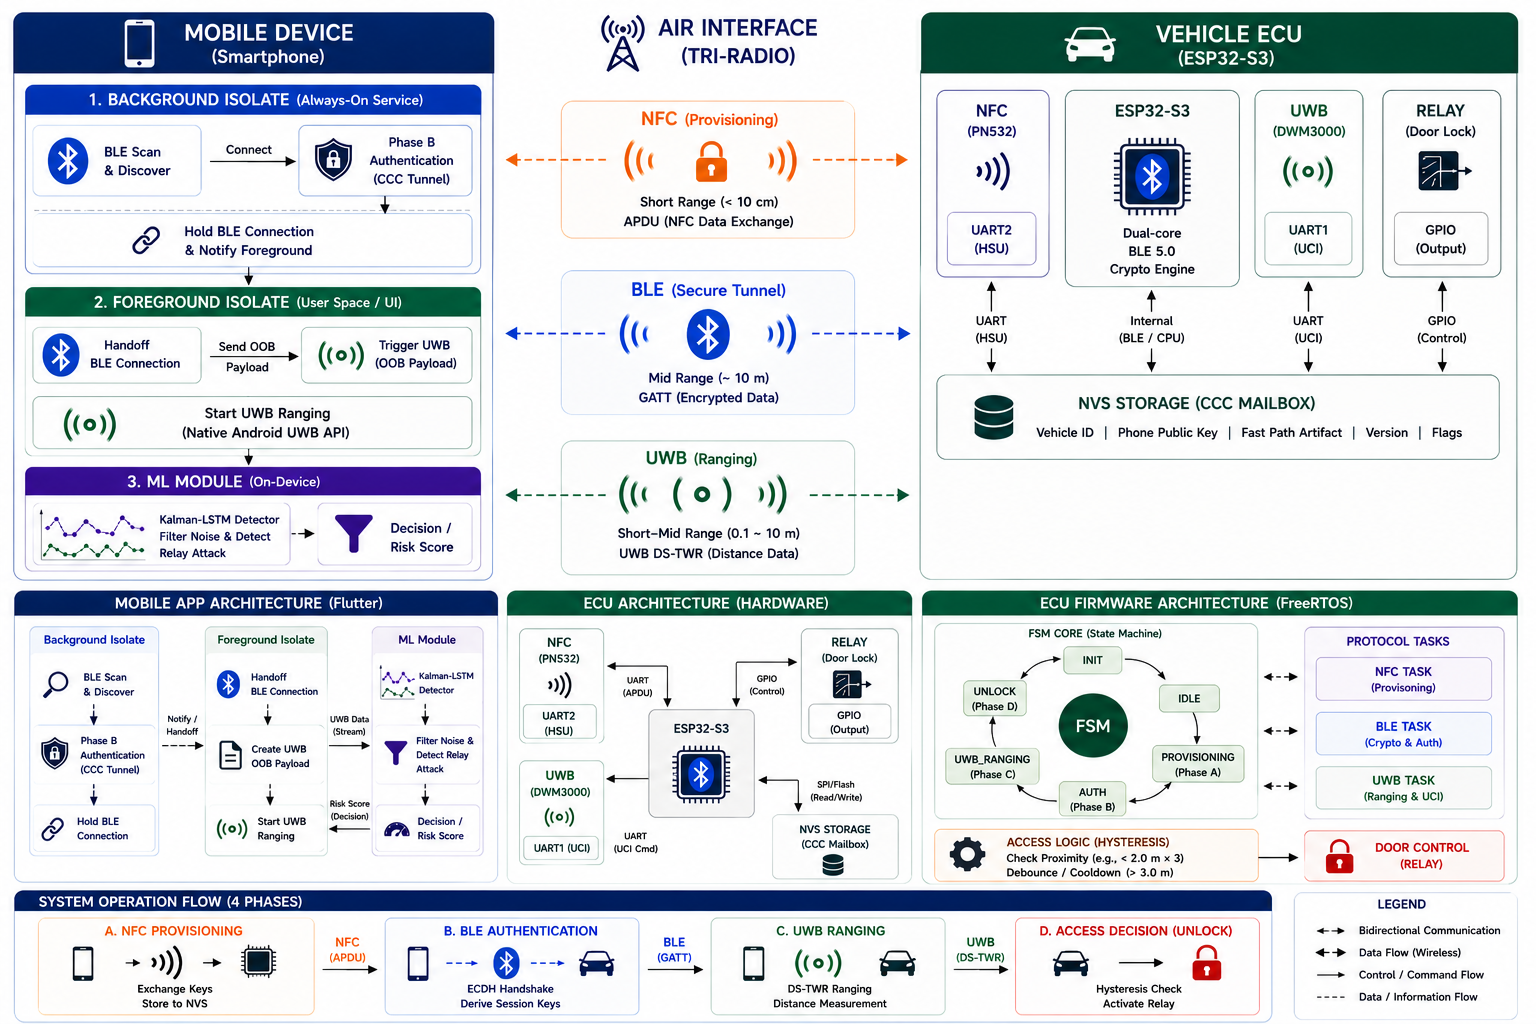
\includegraphics[width=1.0\textwidth]{image/section4/archi1.png} 
    \caption{Sơ đồ khối kiến trúc hệ thống Smart Car Access Tri-Radio}
    \label{fig:block_diagram}
\end{figure}

\subsection{Kiến trúc phần cứng ECU}

Hệ thống phần cứng trên xe được thiết kế module hóa nhằm tối ưu hóa hiệu năng giao tiếp đa kênh, bao gồm các thành phần:
\begin{itemize}
    \item \textbf{Core Microcontroller:} Vi điều khiển ESP32-S3 (Dual-core, tích hợp phần cứng mã hóa và BLE 5.0).
    \item \textbf{NFC Subsystem:} Sử dụng module PN532 phục vụ quá trình cấp quyền (Provisioning). Giao tiếp với ESP32 qua UART2 (RX=Pin 44, TX=Pin 43) sử dụng chế độ High Speed UART (HSU) ở tốc độ baud 115200.
    \item \textbf{UWB Subsystem:} Sử dụng vi mạch DWM3000 (được điều khiển bởi chip nRF52840 chạy UCI protocol firmware) để đo khoảng cách an toàn (Distance Bounding). Giao tiếp với ESP32 qua UART1 (RX=Pin 17, TX=Pin 18) thông qua giao thức UWB Command Interface (UCI).
    \item \textbf{Actuator (Cơ cấu chấp hành):} Module Relay khóa cửa, được điều khiển trực tiếp bởi chân GPIO (Digital Output) của ESP32.
\end{itemize}

\subsection{Kiến trúc phần mềm di động}

Để hiện thực hóa tính năng "Mở khóa không chạm" (Passive Keyless Entry) mà không làm tiêu hao tài nguyên pin, ứng dụng Flutter được chia thành hai không gian bộ nhớ (Isolates) tách biệt cùng với một module Trí tuệ nhân tạo:

\begin{itemize}
    \item \textbf{Background Isolate (Luồng chạy ngầm):} Quản lý bởi \texttt{PkeBackgroundService}. Nhiệm vụ của luồng này là liên tục quét (Scan) tín hiệu BLE dưới nền. Khi phát hiện xe, luồng tự động thiết lập kênh truyền an toàn và thực hiện Xác thực mật mã (Phase B). Điểm mấu chốt là sau khi xác thực, luồng này \textit{không ngắt kết nối} mà tiến hành "Giữ trạng thái" (Hold Connection) để bàn giao cho luồng Foreground.
    \item \textbf{Foreground Isolate (Luồng giao diện \& UWB Handoff):} Xử lý dịch vụ \texttt{UwbService} thông qua Native Android MethodChannel (\texttt{smartcar/uwb}). Kế thừa kết nối BLE từ Background, luồng này tạo gói tin OOB (Out-of-band Payload), gửi qua BLE Admin Characteristic (0x0005) cho ESP32, sau đó kích hoạt chip UWB trên điện thoại để bắt đầu phiên đo khoảng cách (Ranging).
    \item \textbf{Security \& ML Module:} Chứa thuật toán \textit{Kalman-LSTM Detector}. Tích hợp chức năng lọc nhiễu tọa độ UWB và phát hiện tấn công tiếp sóng (Relay Attack) dựa trên phân tích sự lạm phát khoảng cách trong chuỗi thời gian (Distance Inflation).
\end{itemize}

\subsection{Kiến trúc phần mềm vi điều khiển}

Firmware của ECU được thiết kế theo kiến trúc Event-Driven \& Multi-Tasking (Hướng sự kiện và Đa luồng) trên hệ điều hành thời gian thực FreeRTOS, đảm bảo xử lý đồng thời ba sóng vô tuyến mà không xảy ra nghẽn cổ chai.

\begin{itemize}
    \item \textbf{Core State Machine (Bộ não trung tâm - FSM Task):} Chạy trên một luồng riêng biệt, FSM quản lý toàn bộ vòng đời hệ thống (\texttt{INIT} $\rightarrow$ \texttt{IDLE} $\rightarrow$ \texttt{PROVISIONING} $\rightarrow$ \texttt{AUTH} $\rightarrow$ \texttt{UWB\_RANGING} $\rightarrow$ \texttt{UNLOCK}). FSM thu thập các sự kiện từ các task phần cứng và đưa ra quyết định chuyển trạng thái xuyên tầng (Cross-layer Security).
    \item \textbf{NFC Task:} Quản lý giao tiếp APDU với điện thoại trong Phase A, trao đổi khóa công khai và thiết lập các tham số Fast Path Artifact.
    \item \textbf{BLE Task (Crypto Engine):} Hoạt động trên nền thư viện NimBLE, cung cấp CCC Auth Service và Admin Service. Task này chịu trách nhiệm tính toán mật mã (mbedTLS): tạo cặp khóa ECDH Ephemeral, tính Shared Secret, băm HKDF-SHA256 sinh Session Keys, và xác thực chữ ký ECDSA.
    \item \textbf{UWB Task:} Quản lý giao thức UCI qua UART1 để cấu hình chip DWM3000, liên tục phân tích gói tin UCI Ranging Notification để trích xuất giá trị khoảng cách (\texttt{distanceM}) và trạng thái.
    \item \textbf{Door Unlock Module (Hysteresis Logic):} Đảm nhiệm quyết định mở cửa. Thuật toán yêu cầu khoảng cách đo được phải $\le 2.0$m trong 3 chu kỳ đo liên tiếp (Debounce) mới kích hoạt GPIO, và chỉ reset khi điện thoại ra khỏi vùng an toàn ($> 3.0$m).
    \item \textbf{CCC Mailbox:} Quản lý bộ nhớ Non-Volatile Storage (NVS) để lưu trữ tĩnh ID Xe, Public Key của điện thoại và các thông số cài đặt.
\end{itemize}

\begin{table}[H]
\centering
\begin{tabular}{|p{7.2cm}|p{7.2cm}|}
\hline
\textbf{Mobile App (Flutter Dual-Isolate)} & \textbf{Vehicle Controller (C/C++ FreeRTOS)} \\ \hline
\textbf{Background Isolate:} Quét BLE ngầm, tự động kết nối và chạy Phase B (Crypto) không cần mở màn hình. & \textbf{FSM Core:} Máy trạng thái hữu hạn kiểm soát tính nhất quán xuyên tầng (Cross-layer). \\ \hline
\textbf{Foreground Isolate:} Nhận Handoff, gọi API Native Android cấu hình chip UWB và gửi OOB. & \textbf{Tasks \& Protocol Layer:} NFC Task (APDU), BLE Task (GATT/Crypto), UWB Task (UCI Protocol). \\ \hline
\textbf{ML Layer:} Bộ lọc Kalman-LSTM phát hiện Relay Attack từ dữ liệu thô. & \textbf{Access Logic:} Thuật toán Hysteresis kết hợp dữ liệu Ranging để điều khiển GPIO Relay. \\ \hline
\end{tabular}
\caption{Tương quan kiến trúc phần mềm giữa Mobile App và ECU}
\label{tab:sw_arch_new}
\end{table}

\subsection{Luồng tương tác xuyên tầng}

Để đảm bảo an ninh vật lý và logic, hệ thống thực thi chuỗi giao dịch xuyên qua ba giao thức độc lập theo trình tự nghiêm ngặt sau:

\begin{enumerate}
    \item \textbf{Phase A: Cấp phép vật lý (Physical Root-of-Trust) - NFC} \\
    Đầu tiên người dùng thêm thông tin xe bằng cách sử dụng app quét thẻ master card, Sau đó người dùng chạm điện thoại vào NFC Reader. \texttt{NFCTask} nhận diện thẻ HCE, chuyển FSM sang trạng thái \texttt{PROVISIONING}. Hai thiết bị trao đổi Public Keys và lưu vào \texttt{CCCMailbox}.
    
    \item \textbf{Phase B: Xác thực bảo mật (Cryptographic Session Binding) - BLE} \\
    Khi người dùng tiến vào vùng Welcome Zone ($\sim 10$m), \texttt{PkeBackgroundService} tự động kết nối BLE. ESP32 chuyển FSM sang \texttt{AUTH}. Hai bên sinh khóa tạm thời ECDH, ký xác nhận bằng khóa NFC đã lưu, dẫn xuất ra các Khóa phiên (Session Keys).
    
    \item \textbf{Phase C: Xác thực khoảng cách (Physical Distance Bounding) - UWB} \\
    Sau khi Phase B thành công, điện thoại gửi cấu hình UWB (OOB Payload) qua đường hầm BLE. ESP32 đẩy OOB sang \texttt{UWBTask} để bật vi mạch DWM3000. Giao thức DS-TWR (Double-Sided Two-Way Ranging) hoạt động, liên tục trả về các thông số khoảng cách ($1.5$m, $1.3$m, $0.8$m...).
    
    \item \textbf{Phase D: Quyết định mở cửa (Conjunctive Access Decision)} \\
    Dữ liệu khoảng cách từ Phase C được đẩy vào mạng lọc Hysteresis. Nếu hệ thống ghi nhận 3 lần liên tiếp khoảng cách $< 2.0$m \textbf{VÀ} FSM đang ở trạng thái \texttt{AUTH\_SECURE\_CHANNEL\_READY} (Đã xác thực BLE), ESP32 mới cấp điện cho GPIO kích hoạt Relay mở cửa.
\end{enumerate}







%------------------------------------------------------------------------------------







\section{Lựa chọn nền tảng phần cứng}

Việc lựa chọn phần cứng đóng vai trò then chốt trong việc hiện thực hóa các giao thức bảo mật phức tạp và xử lý đồng thời đa vô tuyến trong thời gian thực.

\subsection{Yêu cầu về phần cứng trung tâm}
Bộ điều khiển trung tâm cần đáp ứng các tiêu chí:
\begin{itemize}
    \item Hỗ trợ cấu hình nhiều giao tiếp ngoại vi độc lập (UART/SPI) để kết nối NFC và UWB mà không nghẽn cổ chai.
    \item Có khả năng xử lý các thuật toán mã hóa (ECDH, ECDSA, AES), ưu tiên có bộ tăng tốc phần cứng (Hardware Accelerator).
    \item Có bộ nhớ lưu trữ không bay hơi (NVS) và đủ dung lượng RAM cho RTOS đa luồng.
\end{itemize}

\subsection{Phân tích và lựa chọn: Automotive ECU vs. ESP32-S3}

\subsubsection{Target Platform: Automotive ECU}
Các ECU tiêu chuẩn công nghiệp (như Bosch EDC17, Continental BCM) sử dụng kiến trúc ARM Cortex-M4/M7, tuân thủ chuẩn AUTOSAR và ISO 26262. Tuy nhiên, rào cản lớn nhất đối với nghiên cứu là chi phí đắt đỏ (\$500-\$2000/unit) và độ phức tạp cực kỳ cao trong việc tiếp cận công cụ phát triển (Vector CANoe).

\subsubsection{Development Platform: ESP32-S3}
Nhóm quyết định sử dụng ESP32-S3 làm nền tảng phát triển Proof-of-Concept (PoC) dựa trên các lợi thế kỹ thuật chuyên sâu \cite{esp32s3}:

\textbf{A. Thông số kỹ thuật ESP32-S3:}
\begin{itemize}
    \item \textbf{MCU:} Xtensa LX7 dual-core hoạt động ở xung nhịp 240 MHz, cung cấp năng lực xử lý vượt trội.
    \item \textbf{Crypto Engine:} Tích hợp bộ tăng tốc phần cứng cho AES, SHA, RSA, RNG.
    \item \textbf{Wireless:} Tích hợp sẵn Wi-Fi và BLE 5.0 Native.
    \item \textbf{Peripherals:} Hỗ trợ ma trận phần cứng linh hoạt, cho phép cấu hình 2 luồng UART độc lập (UART1 cho DWM3000, UART2 cho PN532) không xung đột.
\end{itemize}

\textbf{B. So sánh kỹ thuật chi tiết:}

\begin{table}[H]
\centering
\begin{tabularx}{\textwidth}{|l|X|X|X|}
\hline
\textbf{Tiêu chí} & \textbf{Automotive ECU} & \textbf{ESP32-S3} & \textbf{Đánh giá} \\ \hline
Processing Power & ARM M4/M7 & Xtensa LX7 @240MHz & Tương đương \\ \hline
Crypto HW & Có & Có (AES, SHA Accel) & Đạt yêu cầu \\ \hline
Kết nối nội bộ & Multi-bus & Ma trận linh hoạt (Multi-UART) & Rất phù hợp cho UWB/NFC \\ \hline
Chi phí & \$500 - \$2000 & $\approx$ \$5 & ESP32 tối ưu \\ \hline
Safety Cert & ISO 26262 & Không có & Hạn chế của ESP32 \\ \hline
Development & Phức tạp (AUTOSAR) & Linh hoạt (FreeRTOS/C++) & ESP32 dễ tiếp cận \\ \hline
\end{tabularx}
\caption{So sánh Automotive ECU và ESP32-S3}
\end{table}

\textbf{C. Kết quả Benchmark hiệu năng Crypto:}
Để chứng minh khả năng đáp ứng thời gian thực (đặc biệt khi kết hợp luồng đo UWB), nhóm đã thực hiện đo đạc trên ESP32-S3 (sử dụng thư viện mbedTLS):
\begin{itemize}
    \item ECDH key exchange (P-256): \textbf{85ms} (Mục tiêu $< 100$ms).
    \item ECDSA verify (P-256): \textbf{95ms}.
    \item AES-128-GCM encrypt (1KB): \textbf{12ms}.
    \item \textbf{Tổng thời gian luồng xác thực BLE:} \textbf{< 400ms} (Dư dả thời gian cấp quyền bật UWB).
\end{itemize}

\textbf{Kết luận:} ESP32-S3 hoàn toàn đáp ứng được các yêu cầu khắt khe về thời gian phản hồi, khả năng quản lý đa luồng FreeRTOS cho giao thức Tri-Radio, đồng thời tối ưu hóa thời gian và chi phí phát triển R\&D.

\subsection{Kiến trúc chuyển đổi}
Để đảm bảo tính khả thi khi chuyển đổi từ ESP32 sang ECU thực tế trong tương lai, hệ thống phần mềm được thiết kế theo kiến trúc phân lớp (Layered Architecture):

\begin{itemize}
    \item \textbf{Application Layer:} Chứa logic FSM, Access Control. Tầng này độc lập với phần cứng.
    \item \textbf{Protocol Layer:} Xử lý APDU, BLE GATT, UCI Parser. Tuân thủ tiêu chuẩn quốc tế.
    \item \textbf{Hardware Abstraction Layer (HAL):} Tầng trung gian quản lý UART/GPIO. Hiện tại HAL map vào ESP-IDF, trong tương lai có thể map vào AUTOSAR BSW \cite{iso26262}.
\end{itemize}

Việc tách biệt này giúp tái sử dụng phần lớn mã nguồn C/C++ khi thay đổi phần cứng vi điều khiển.





%------------------------------------------------------------------------------------





\section{Thiết kế giao thức bảo mật}

Kiến trúc bảo mật của hệ thống được thiết kế phân lớp, tuân thủ nghiêm ngặt chuẩn CCC Digital Key Release 3.0 nhằm triệt tiêu các rủi ro tấn công tiếp sóng và giả mạo thiết bị. Quá trình từ khi người dùng chưa có quyền đến khi mở cửa xe thành công được chia thành 4 giai đoạn (Phases) với trách nhiệm bảo mật chuyên biệt.

\subsection{Phase A - Giai đoạn Cấp quyền vật lý}
Phase A thiết lập mối quan hệ tin cậy nền tảng (Root-of-Trust) giữa điện thoại thông minh và ECU của xe thông qua kênh giao tiếp vật lý tầm ngắn NFC (Out-of-Band). Sự giới hạn về khoảng cách của NFC ($< 10$cm) chính là lớp khiên vật lý chống lại các hành vi nghe lén.

\leavevmode
\begin{figure}[htbp]
    \centering
    % Sinh viên lưu ý cập nhật ảnh Sơ đồ kiến trúc mới có đủ NFC, BLE, UWB và luồng Dual-Isolate nhé
    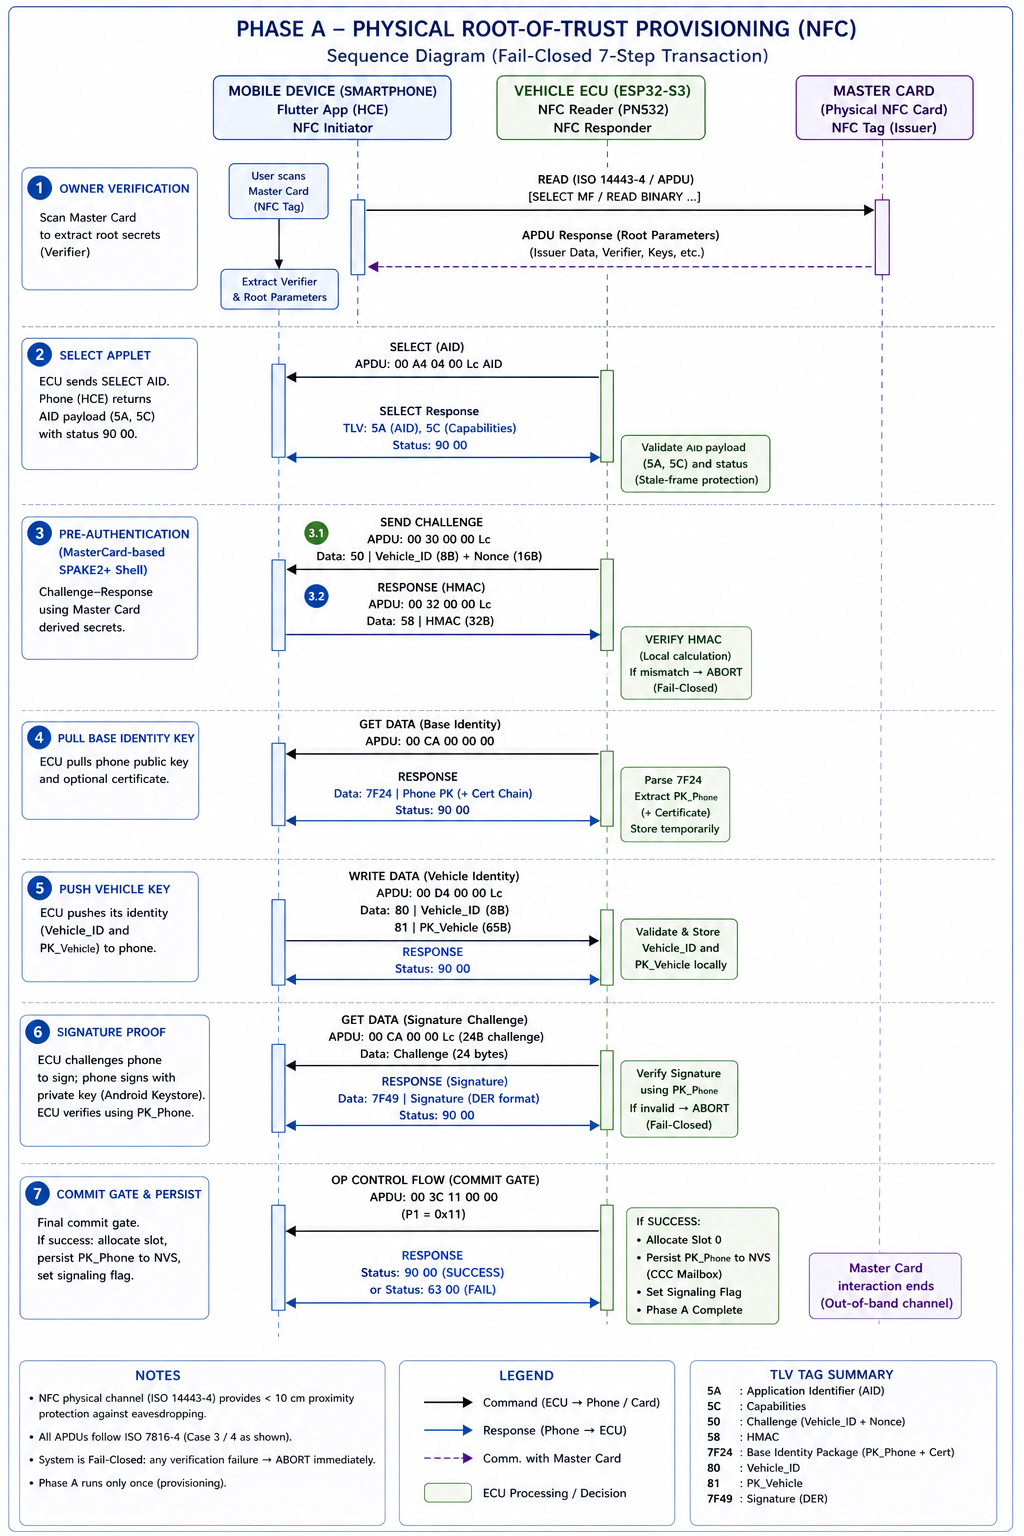
\includegraphics[width=0.9\textwidth]{image/section4/phaseAnew.png} 
    \caption{Sơ đồ Sequence Phase A}
    \label{fig:phaseA}
\end{figure}

Nhằm tăng cường độ tin cậy và chống lại các khung dữ liệu cũ/trễ (Stale-frame), hệ thống không sử dụng luồng cấp quyền đơn giản mà áp dụng một quy trình giao dịch \textit{Fail-Closed} nghiêm ngặt gồm 7 bước:

\begin{enumerate}
    \item \textbf{Xác thực quyền sở hữu qua thẻ Master Card (Owner Verification):} 
    Trước khi tương tác với xe, người dùng phải sử dụng điện thoại thông minh để quét thẻ NFC vật lý Master Card (thẻ gốc do nhà sản xuất cấp) thông qua đầu đọc NFC tích hợp trên điện thoại. Bước này giúp ứng dụng trích xuất các tham số mật mã nền tảng (Verifier) nhằm chứng minh người dùng là chủ sở hữu hợp pháp của phương tiện trước khi bắt đầu quy trình cấp quyền.

    \item \textbf{Lựa chọn Applet (SELECT AID):} 
    Người dùng đưa điện thoại (lúc này đang kích hoạt chế độ mô phỏng thẻ HCE) chạm vào đầu đọc NFC (PN532) trên xe. ECU lập tức gửi lệnh \texttt{SELECT AID} chuẩn ISO 7816-4. Ứng dụng HCE trên điện thoại phản hồi các thẻ dữ liệu (payload tags \texttt{5A, 5C}) kèm mã trạng thái \texttt{90 00}. ECU thực hiện xác thực chéo nội dung payload nhằm loại bỏ hoàn toàn các khung dữ liệu rác (Stale-frame protection).

    \item \textbf{Xác thực sơ bộ (MasterCard-based SPAKE2+ Shell):} 
    Hệ thống áp dụng cơ chế xác thực mô phỏng chuẩn MasterCard để xác minh dữ liệu quét được từ bước 1. ESP32 tạo một thông điệp thử thách (Challenge) gồm định danh xe (\texttt{Vehicle\_ID} - 8 bytes) và chuỗi ngẫu nhiên (Nonce - 16 bytes). 
    \begin{itemize}
        \item ECU gửi Challenge qua lệnh APDU \texttt{0x30} (được bọc trong thẻ TLV \texttt{0x50}).
        \item Điện thoại sử dụng thông tin từ thẻ Master Card để tính toán, sau đó phản hồi lệnh yêu cầu xác thực \texttt{0x32} bằng mã băm HMAC (thẻ TLV \texttt{0x58}). 
        \item ESP32 tính toán HMAC cục bộ và đối chiếu. Nếu dữ liệu không khớp hoàn toàn, giao dịch lập tức bị hủy.
    \end{itemize}

    \item \textbf{Rút khóa định danh cơ sở (Base Key Exchange Pull):} 
    ECU gửi lệnh \texttt{GET DATA} (INS \texttt{0xCA}, \texttt{Lc=0}). Điện thoại trả về gói định danh cơ sở (bọc bởi tag \texttt{7F24}). ESP32 tiến hành phân tách gói tin để thu thập Khóa công khai của điện thoại ($PK_{Phone}$) và chuỗi chứng chỉ tùy chọn.

    \item \textbf{Đẩy khóa định danh xe (Vehicle Key Exchange Push):} 
    Để thiết lập ràng buộc hai chiều, ECU chủ động gửi lệnh \texttt{WRITE DATA} (INS \texttt{0xD4}) đẩy dữ liệu sang điện thoại. Các tham số bao gồm \texttt{Vehicle\_ID} (TLV \texttt{0x80}) và Khóa công khai của xe $PK_{Vehicle}$ (TLV \texttt{0x81}). Ứng dụng điện thoại sẽ xác thực và lưu trữ các tham số này cục bộ.

    \item \textbf{Chứng minh bằng chữ ký (Signature Proof):} 
    ECU gửi một lệnh \texttt{GET DATA} (INS \texttt{0xCA}) thứ hai mang theo một Challenge dài 24 bytes vào vùng dữ liệu APDU. Điện thoại bắt buộc phải ký chuỗi này bằng Private Key được bảo vệ sâu trong Android Keystore và trả về chữ ký định dạng DER. ESP32 sử dụng $PK_{Phone}$ vừa nhận được ở bước 4 để xác thực chữ ký này.

    \item \textbf{Cổng cam kết và Lưu trữ (Commit Gate \& Persist):} 
    Nếu chữ ký hoàn toàn hợp lệ, ECU tiến hành gửi lệnh \texttt{OP CONTROL FLOW} (INS \texttt{0x3C}, tham số \texttt{P1=0x11}) làm "Cổng cam kết" cho giao dịch. Chỉ khi bước chốt chặn này báo thành công, ESP32 mới cấp phát Slot 0, lưu trữ vĩnh viễn $PK_{Phone}$ vào bộ nhớ bảo mật NVS (CCC Mailbox) và bật cờ tín hiệu (Signaling flag). Phase A chính thức kết thúc.
\end{enumerate}

Phase A chỉ diễn ra một lần duy nhất. Giai đoạn này không thực hiện mở khóa xe mà đóng vai trò gieo mầm (Seeding) các khóa định danh dài hạn cho các pha xác thực vô tuyến tiếp theo.

\subsection{Phase B - Xác thực bảo mật kênh truyền}
Giai đoạn B thiết lập một đường hầm bảo mật (Secure Tunnel) tầm xa giữa điện thoại và xe qua sóng Bluetooth Low Energy (BLE). Mục tiêu của Phase B \textbf{không phải là mở cửa xe}, mà là để chứng minh quyền sở hữu khóa (Proof of Ownership) và sinh ra các khóa phiên (Session Keys).

\leavevmode
\begin{figure}[htbp]
    \centering
    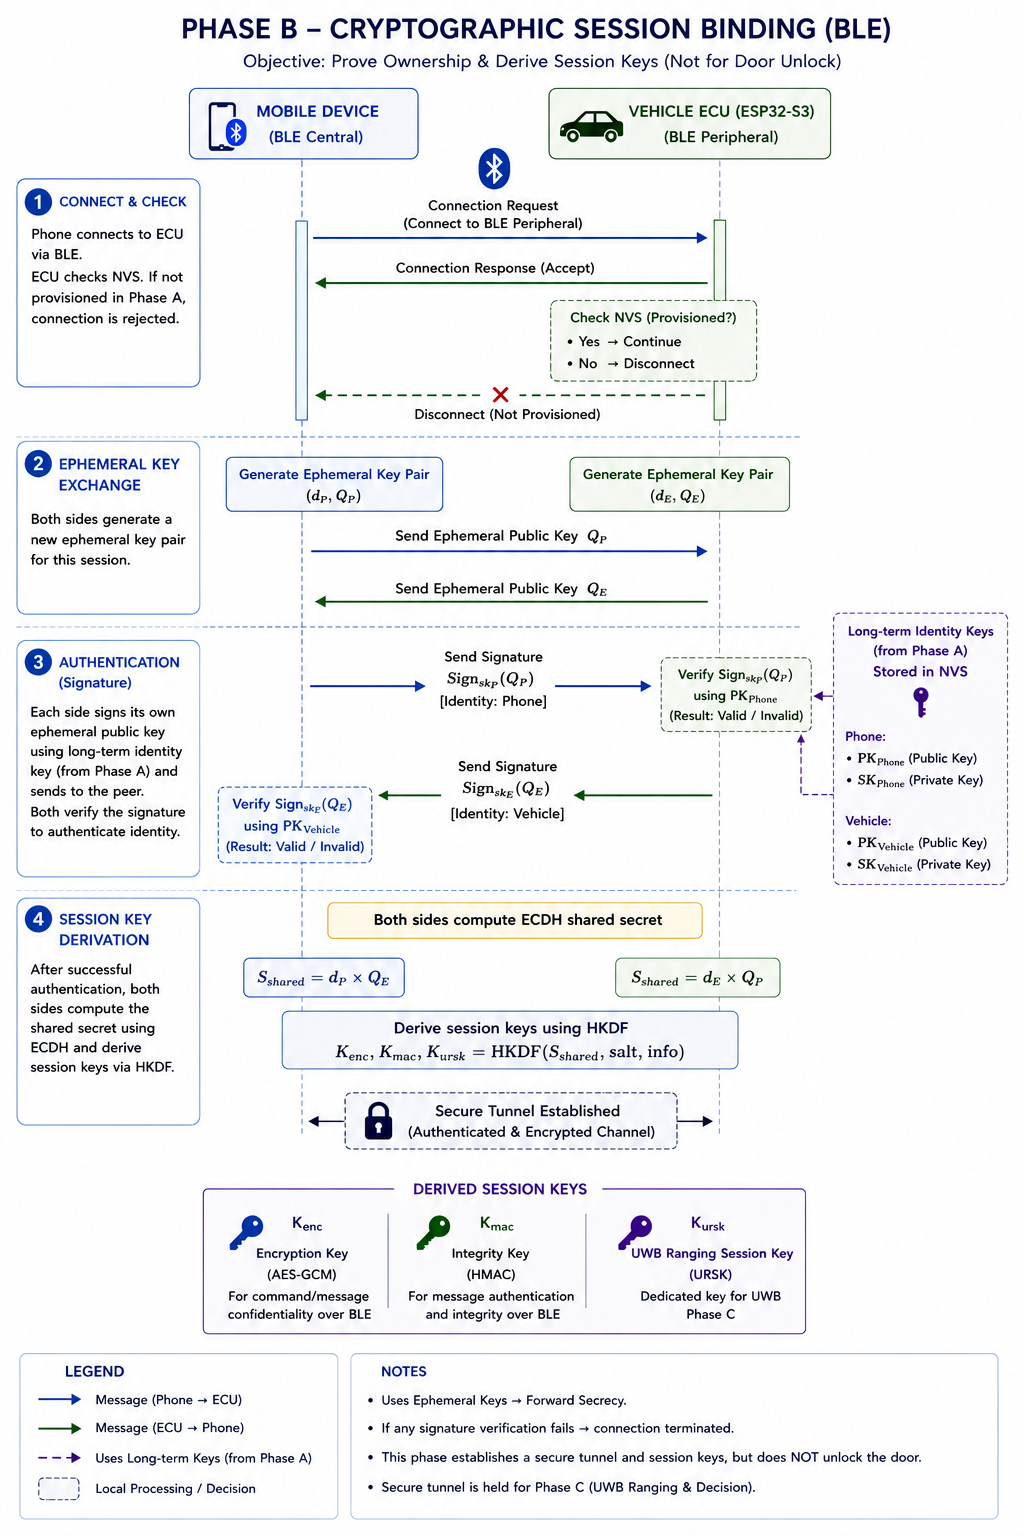
\includegraphics[width=0.9\textwidth]{image/section4/phaseBnew.png} 
    \caption{Sơ đồ Sequence Phase B}
    \label{fig:phaseB}
\end{figure}

\textbf{Quy trình bắt tay 3 bước (3-Way Handshake) dựa trên ECDH:}
\begin{enumerate}
    \item \textbf{Kết nối và Kiểm tra:} Điện thoại (BLE Central) tiến vào vùng phủ sóng và kết nối với ESP32 (BLE Peripheral). ESP32 kiểm tra trạng thái NVS, nếu chưa được Provisioning ở Phase A, kết nối lập tức bị ngắt.
    \item \textbf{Trao đổi khóa tạm thời (Ephemeral Key Exchange):} Cả hai thiết bị sinh một cặp khóa đường cong Elliptic tạm thời (Ephemeral Keys) hoàn toàn mới cho phiên kết nối hiện tại.
    \item \textbf{Xác thực danh tính (Authentication):} Mỗi bên dùng Khóa định danh dài hạn (đã lưu ở Phase A) để ký lên Khóa tạm thời của mình rồi gửi cho đối phương. Quá trình này giúp hai bên xác minh chắc chắn danh tính của nhau.
    \item \textbf{Dẫn xuất khóa phiên (Session Key Derivation):} Sau khi xác thực chữ ký, hai bên dùng thuật toán ECDH để tính ra bí mật chung ($S_{shared}$). Từ đó, sử dụng hàm KDF (Key Derivation Function) \cite{rfc5869} để sinh ra các khóa dùng một lần:
\end{enumerate}

\begin{equation}
    K_{enc}, K_{mac}, K_{ursk} = \text{HKDF}(S_{shared}, \text{salt}, \text{info})
\end{equation}

Trong đó:
\begin{itemize}
    \item $K_{enc}, K_{mac}$: Khóa dùng để mã hóa (AES-GCM) và xác thực toàn vẹn (HMAC) các thông điệp lệnh qua BLE \cite{fips197}.
    \item $K_{ursk}$: Khóa Ranging Session Key dành riêng cho giao thức UWB ở Phase C \cite{neirynck2016overview}.
\end{itemize}

Việc sử dụng Ephemeral Keys đảm bảo tính \textbf{Bảo mật chuyển tiếp (Forward Secrecy)}: Dù kẻ gian có giải mã được khóa của một phiên kết nối cũ, chúng cũng không thể can thiệp vào các phiên kết nối hiện tại hay tương lai.

\subsection{Phase C - Xác thực khoảng cách an toàn với UWB}
Khác với các hệ thống Smart Key truyền thống dùng RSSI của Bluetooth để đo khoảng cách (vốn dễ bị khuyếch đại bởi các bộ lặp Relay), hệ thống sử dụng công nghệ UWB (Ultra-Wideband) làm thước đo vật lý chính xác tuyệt đối.

\leavevmode
\begin{figure}[htbp]
    \centering
    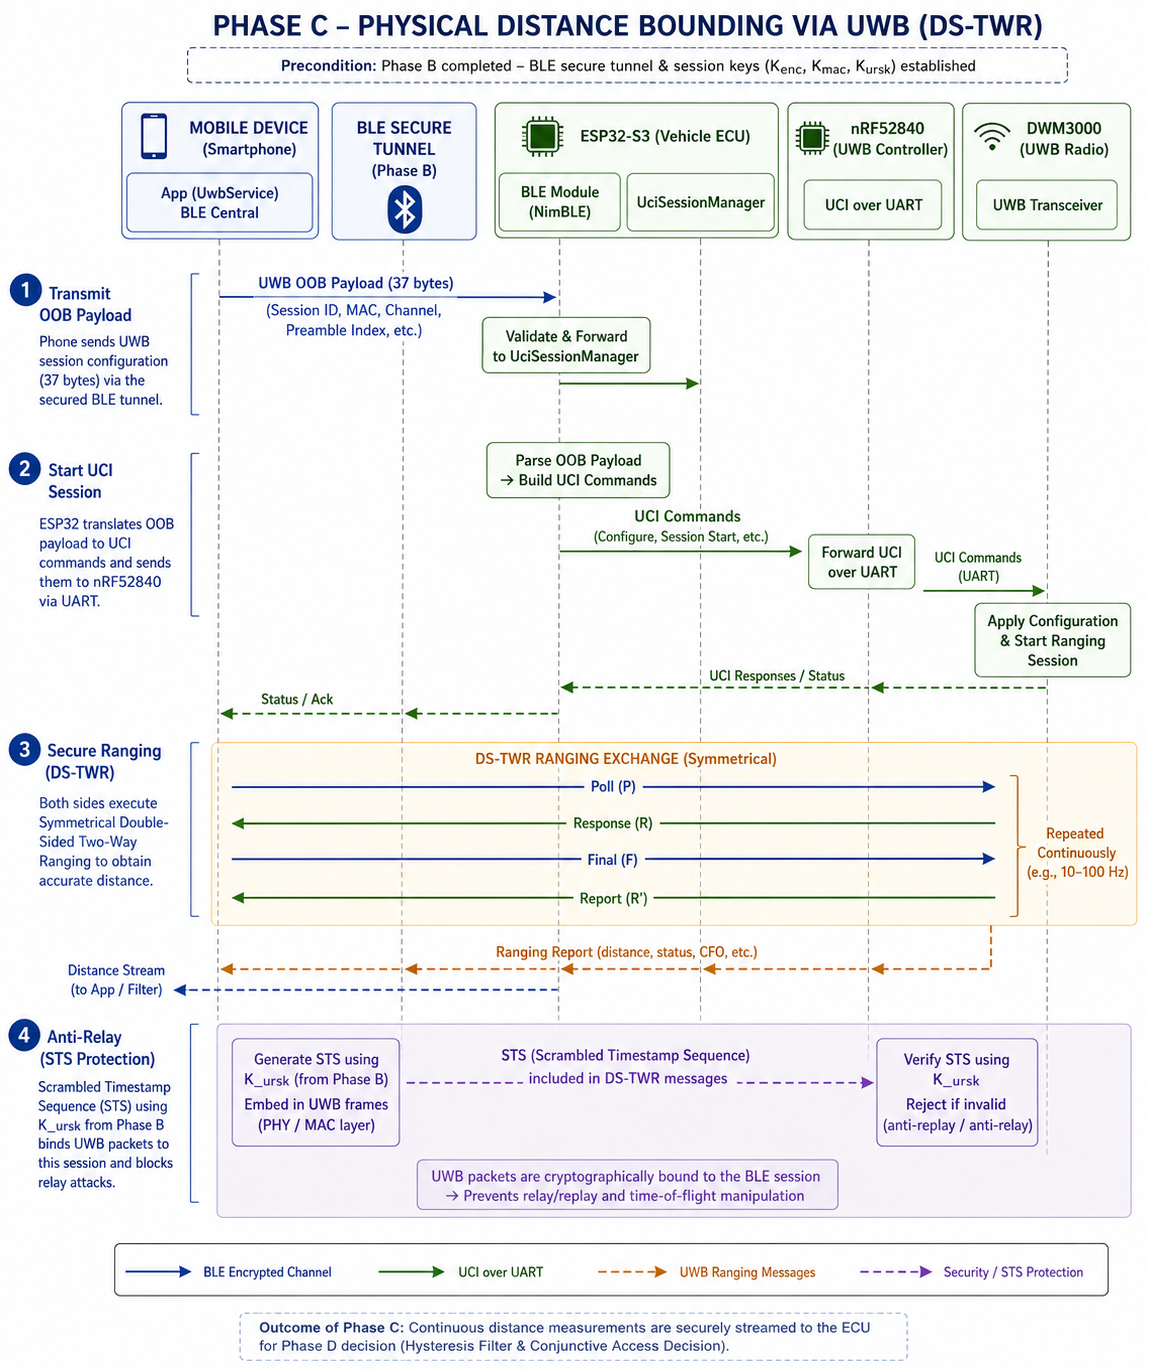
\includegraphics[width=0.9\textwidth]{image/section4/phaseCnew.png} 
    \caption{Sơ đồ Sequence Phase C}
    \label{fig:phaseC}
\end{figure}

\begin{enumerate}
    \item \textbf{Truyền OOB Payload:} Thông qua đường hầm BLE đã được bảo mật ở Phase B, điện thoại gửi một gói \textit{Out-Of-Band (OOB) Payload} (37 bytes) chứa cấu hình phiên UWB (Session ID, MAC Address, Channel, Preamble Index) đến ESP32.
    \item \textbf{Khởi động phiên UCI:} ESP32 (lớp \texttt{UciSessionManager}) dịch OOB Payload thành các lệnh UWB Command Interface (UCI) và đẩy xuống vi mạch nRF52840 gắn shield DWM3000 thông qua giao tiếp UART1. Từ đó Ranging session sẽ được thiết lập.
    \item \textbf{Đo khoảng cách (Secure Ranging):} Vi mạch UWB hai bên bắt đầu phát xung. Giao thức \textbf{Symmetrical Double-Sided Two-Way Ranging (DS-TWR)} được sử dụng nhằm triệt tiêu hoàn toàn sai số trôi đồng hồ (Clock drift) giữa điện thoại và xe.
    \item \textbf{Chống Relay Attack:} Để ngăn chặn kẻ gian thu phát lại tín hiệu xung UWB, một chuỗi dấu thời gian bị xáo trộn (Scrambled Timestamp Sequence - STS) được áp dụng vào tầng vật lý (MAC layer) \cite{ccc_digikey3, nxp_ncj29d5, neirynck2016overview}. STS được mã hóa bằng chính khóa $K_{ursk}$ đã sinh ra từ Phase B \cite{neirynck2016overview}. Nhờ đó, gói tin UWB bị ràng buộc chặt chẽ với phiên BLE, triệt tiêu mọi khả năng chèn ép hoặc làm giả thời gian bay (Time-of-Flight).
\end{enumerate}

\subsection{Phase D - Quyết định truy cập thông minh dựa trên học sâu}

Đây là giai đoạn thực thi cuối cùng và quan trọng nhất của hệ thống. Việc kích hoạt rơ-le mở cửa (Door Unlock Actuator) không còn phụ thuộc vào các ngưỡng khoảng cách tĩnh đơn lẻ, mà là kết quả của sự \textbf{quyết định kết hợp} giữa trạng thái giao thức, dữ liệu vật lý thời gian thực và kết quả suy luận từ mô hình học sâu chuỗi thời gian.

\leavevmode
\begin{figure}[htbp]
    \centering
    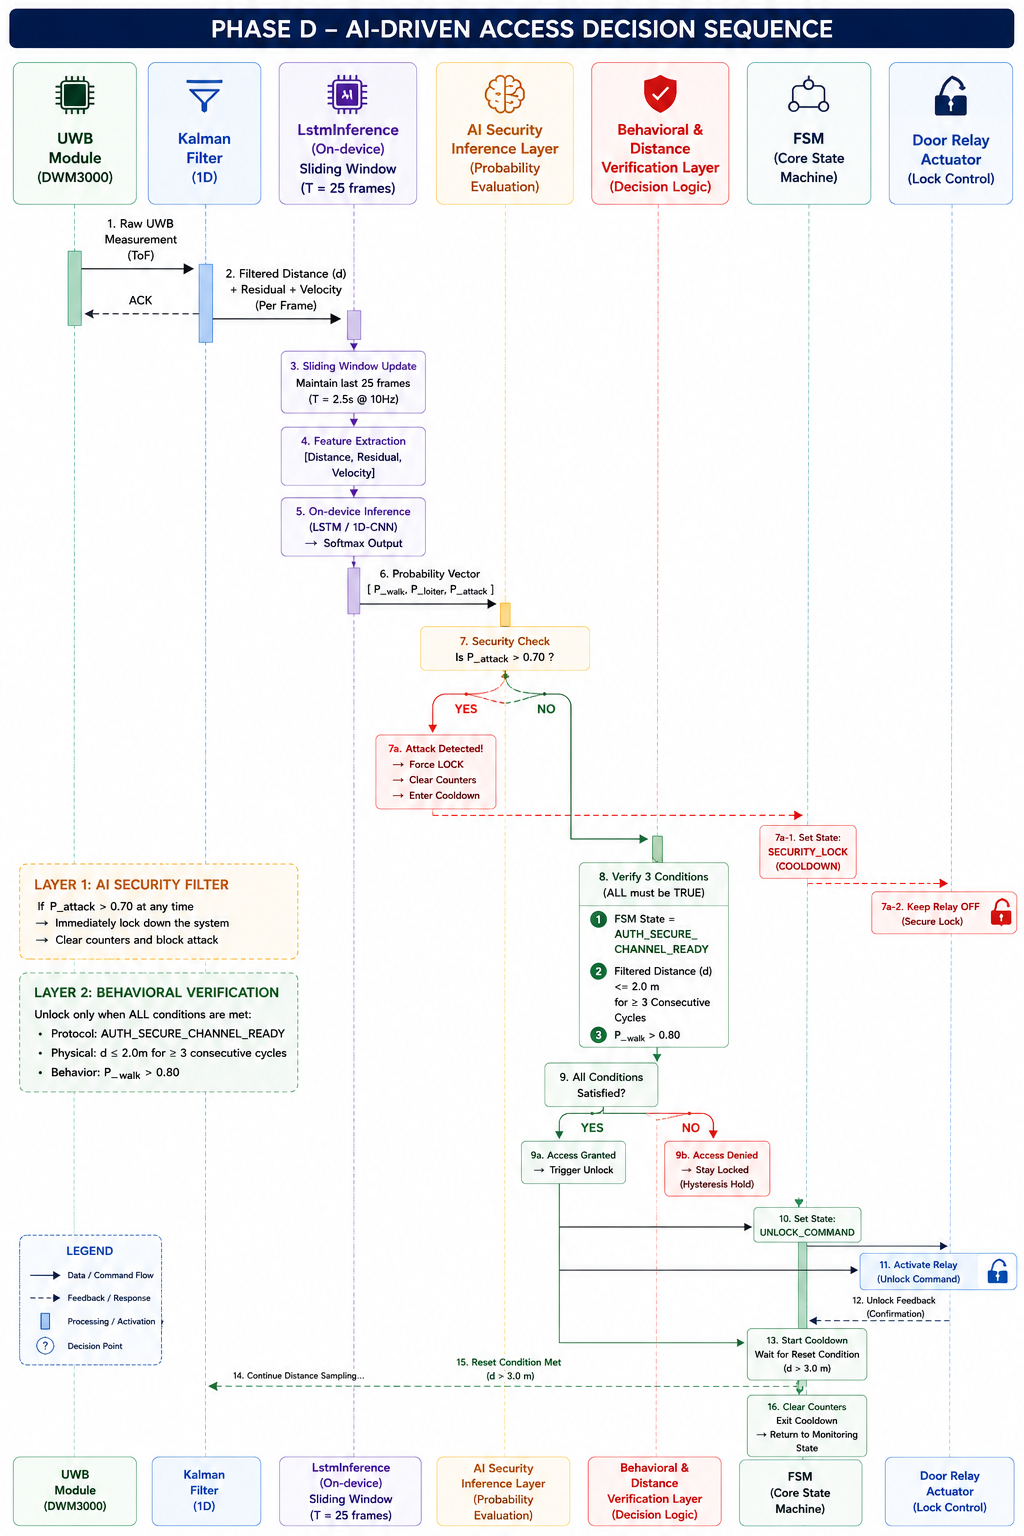
\includegraphics[width=0.8\textwidth]{image/section4/phaseDnew2.png} 
    \caption{Sơ đồ Sequence Phase D tích hợp suy luận AI}
    \label{fig:phaseD}
\end{figure}

Dữ liệu UWB sau khi đi qua bộ lọc Kalman sẽ được đưa vào module \texttt{LstmInference}. Tại đây, một cửa sổ trượt (Sliding Window) lưu trữ $25$ khung hình gần nhất sẽ thực hiện tính toán đặc trưng và suy luận ngay trên vi điều khiển (On-device Inference). Quy trình ra quyết định được thực hiện qua hai lớp bảo mật:

\begin{enumerate}
    \item \textbf{Lớp lọc an ninh AI (Security Inference Layer):}
    Hệ thống liên tục đánh giá vector xác suất từ mô hình AI bao gồm $P_{walk}$ (Tiếp cận), $P_{loiter}$ (Lảng vảng) và $P_{attack}$ (Tấn công tiếp sóng). 
    \begin{itemize}
        \item Nếu ghi nhận xác suất tấn công $P_{attack} > 0.70$, hệ thống lập tức cưỡng bức trạng thái khóa an toàn, ngăn chặn hoàn toàn mọi nỗ lực xâm nhập bằng thiết bị tiếp sóng ngay cả khi khoảng cách vật lý thỏa mãn điều kiện.
    \end{itemize}

    \item \textbf{Lớp xác thực hành vi và khoảng cách (Behavioral Verification Layer):}
    Rơ-le cửa chỉ được phép kích hoạt \textbf{NẾU VÀ CHỈ NẾU} thỏa mãn đồng thời ba điều kiện sau:
    \begin{itemize}
        \item \textbf{Giao thức:} FSM đang ở trạng thái \texttt{AUTH\_SECURE\_CHANNEL\_READY} (Đã xác thực BLE thành công).
        \item \textbf{Vật lý:} Khoảng cách UWB đã lọc ($d$) nằm trong ngưỡng tiệm cận ($\le 2.0$ mét) trong ít nhất \textbf{3 chu kỳ đo liên tiếp}.
        \item \textbf{Hành vi:} Mô hình AI xác nhận ý định người dùng với độ tin cậy $P_{walk} > 0.80$. Điều này giúp loại bỏ hoàn toàn các trường hợp người dùng vô tình đi ngang qua vùng nhận diện hoặc dừng lại ở ranh giới 2m nhưng không có ý định vào xe.
    \end{itemize}
\end{enumerate}

\paragraph*{Điều kiện phục hồi (Cooldown):} 
Sau khi thực hiện lệnh mở cửa, hệ thống sẽ đi vào trạng thái cooldown. Cơ chế Reset chỉ được kích hoạt khi người dùng rời khỏi vùng thiết lập lại (Reset Zone, ví dụ $d > 3.0$ mét), đảm bảo tính ổn định và tránh việc rơ-le hoạt động thừa thãi.

Sự kết hợp giữa lý thuyết điều khiển truyền thống (Hysteresis) và trí tuệ nhân tạo (TinyML) giúp hệ thống Smart Car Access đạt được độ tin cậy vượt trội, mang lại trải nghiệm mở khóa thụ động (PKE) mượt mà nhưng vẫn đảm bảo tính an toàn tuyệt đối trước các hình thức tấn công công nghệ cao hiện nay.

% =======================================================================


\subsection{Cơ chế đánh giá hành vi dựa trên mô hình chuỗi thời gian}

Trong các hệ thống PKE (Passive Keyless Entry) truyền thống, việc ra quyết định mở cửa chỉ dựa trên một ngưỡng khoảng cách tĩnh (ví dụ: $d \le 2.0$m). Tuy nhiên, phương pháp này tồn tại hai lỗ hổng lớn: không thể nhận diện được các bước nhảy vọt của khoảng cách do tấn công tiếp sóng (Relay Attack), và không phân biệt được người dùng đang chủ đích tiến vào xe hay chỉ đang đứng nói chuyện/lảng vảng gần xe (Loitering).

Để giải quyết triệt để bài toán này, kiến trúc hệ thống đã tích hợp thêm một lớp đánh giá hành vi sử dụng mô hình học sâu (Deep Learning) xử lý chuỗi thời gian, vận hành song song với bộ đệm Hysteresis. Cơ chế đánh giá được thực hiện qua các bước sau:

\paragraph*{Cửa sổ thời gian và Trích xuất đặc trưng: }
Thay vì đánh giá từng khung hình rời rạc, hệ thống duy trì một cửa sổ trượt (Sliding Window) có kích thước $T = 25$ khung hình (tương đương với chu kỳ $2.5$ giây ở tần số lấy mẫu 10Hz). Tại mỗi khung hình, bộ tiền xử lý sẽ trích xuất 3 đặc trưng vật lý quan trọng:
\begin{itemize}
    \item \textbf{Khoảng cách đã lọc (Filtered Distance):} Dữ liệu quỹ đạo đi bộ sau khi đi qua bộ lọc Kalman 1D.
    \item \textbf{Thặng dư Kalman (Residual):} Sự chênh lệch giữa phép đo UWB thô và giá trị dự báo của bộ lọc. Đây là đặc trưng tối quan trọng, vì các thiết bị Relay Attack khi khuếch đại tín hiệu sẽ tạo ra độ trễ phần cứng, dẫn đến sự sai lệch đột biến về Thời gian bay (ToF), làm giá trị Residual tăng vọt.
    \item \textbf{Vận tốc tức thời (Velocity):} Đạo hàm bậc 1 của khoảng cách theo thời gian. Đặc trưng này giúp mô hình nhận biết hướng di chuyển (tiến lại gần, lùi ra xa) và trạng thái dừng lại.
\end{itemize}

\paragraph*{Phân loại xác suất hành vi: }
Ma trận dữ liệu đầu vào có kích thước $(25 \times 3)$ sẽ được chuẩn hóa (Z-score Normalization) dựa trên các tham số cấu hình tĩnh (Mean, Scale) từ tập dữ liệu huấn luyện trước khi đưa vào mạng nơ-ron (LSTM/1D-CNN) trên vi điều khiển.
Mô hình sẽ tính toán và xuất ra phân bố xác suất (Softmax) cho 3 kịch bản hành vi:
\begin{itemize}
    \item $P(\text{Walk})$: Xác suất người dùng đang chủ đích bước tới xe.
    \item $P(\text{Loiter})$: Xác suất người dùng đang lảng vảng, đi ngang qua hoặc dừng lại ở ranh giới ngoài mà không có ý định mở cửa.
    \item $P(\text{Attack})$: Xác suất tín hiệu đang bị thao túng bởi trạm lặp (Relay Station).
\end{itemize}

\paragraph*{Tích hợp AI vào Logic điều khiển cơ học: }
Xác suất đầu ra từ mô hình AI không thay thế hoàn toàn cơ chế Hysteresis cơ học mà đóng vai trò như một màng lọc bảo mật cấp cao (High-level Security Gate). Quyết định điều khiển rơ-le mở cửa được thiết kế dựa trên logic kết hợp như sau:
\begin{itemize}
    \item \textbf{Ưu tiên an ninh tuyệt đối:} Nếu bất kỳ thời điểm nào hệ thống ghi nhận $P(\text{Attack}) > 0.70$, hệ thống lập tức từ chối mở cửa và làm trống bộ đệm (Reset counter), vô hiệu hóa hoàn toàn cuộc tấn công.
    \item \textbf{Xử lý nhiễu biên (Edge-case Handling):} Khi người dùng bước vào vùng $< 2.0$m nhưng đột ngột khựng lại hoặc quay lưng bước đi, vận tốc sẽ thay đổi nhanh chóng làm $P(\text{Loiter})$ tăng cao và $P(\text{Walk})$ giảm sút. Rơ-le sẽ không kích hoạt, triệt tiêu hiện tượng mở cửa sai (False Positive).
    \item \textbf{Kích hoạt mở cửa an toàn:} Rơ-le chỉ nhả chốt khi thỏa mãn đồng thời hai điều kiện vật lý và động học: Người dùng đã nằm trong vùng tiệm cận ($d \le 2.0$m) trong 3 chu kỳ đo liên tiếp và AI xác nhận độ tin cậy của hành động tiếp cận ($P(\text{Walk}) > 0.80$).
\end{itemize}

Kết hợp này tạo ra một kiến trúc "Phòng thủ chiều sâu" (Defense-in-depth), nơi thuật toán truyền thống đảm bảo tính an toàn cơ học, còn AI cung cấp lớp bảo mật chống giả mạo vật lý.




%------------------------------------------------------------------------------------








\section{Thiết kế kiến trúc máy trạng thái hữu hạn - FSM}

Trong hệ thống Smart Car Access, máy trạng thái hữu hạn (Finite State Machine - FSM) được sử dụng làm trung tâm điều phối xuyên tầng (Cross-layer Coordinator) để quản lý toàn bộ vòng đời hoạt động của hệ thống. Dựa trên kiến trúc Tri-Radio của chuẩn CCC, FSM phải đồng bộ hóa trạng thái giữa ba tiến trình phần cứng độc lập: NFC (Provisioning - Phase A), BLE (Authentication - Phase B) và UWB (Secure Ranging - Phase C/D) \cite{fsm_book}.

FSM cho phép hệ thống vận hành theo nguyên tắc \textit{Fail-Closed}, có thể kiểm chứng toán học, ngăn chặn các rủi ro bảo mật như tấn công hạ cấp (Downgrade Attack) bằng cách đảm bảo hệ thống không bao giờ bỏ qua các trạng thái xác thực trung gian.

\leavevmode
\begin{figure}[htbp]
    \centering
    % Hãy chèn ảnh FSM Flowchart cập nhật có đủ luồng UWB vào đây
    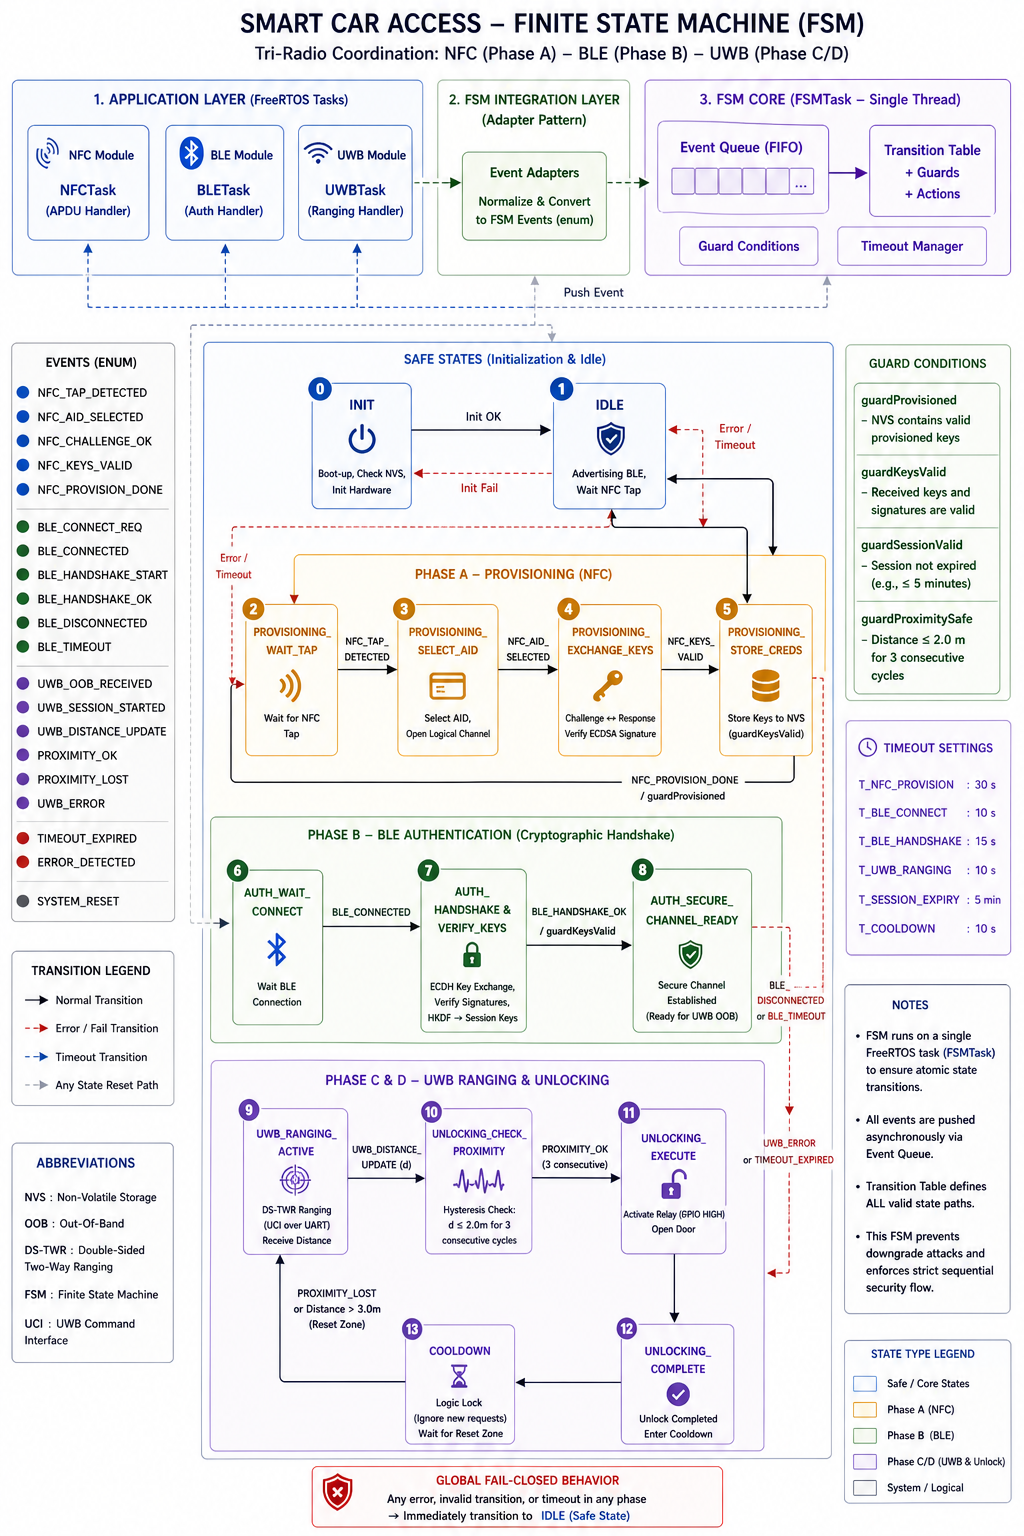
\includegraphics[width=0.9\textwidth]{image/section4/FSMnew.png} 
    \caption{Sơ đồ Máy Trạng thái Xuyên tầng (Cross-layer FSM)}
    \label{fig:fsm_diagram}
\end{figure}

\subsection{Cấu trúc phân lớp FSM}
Kiến trúc FSM trên ESP32 được triển khai dựa trên cơ chế đa luồng (Multi-tasking) của FreeRTOS, bao gồm ba tầng chính:

\begin{enumerate}
  \item \textbf{Tầng Ứng dụng (Application Layer)}: 
  Chạy độc lập trên các FreeRTOS Task tương ứng (\texttt{NFCTask}, \texttt{BLETask}, \texttt{UWBTask}). Tầng này thu thập dữ liệu thô từ các module phần cứng nhưng không có quyền tự thay đổi trạng thái của hệ thống.
  
  \item \textbf{Tầng Tích hợp (FSM Integration Layer)}: 
  Sử dụng Adapter Pattern để chuẩn hóa các sự kiện (Events) riêng lẻ thành dạng enum chung cho FSM (ví dụ: chuyển tín hiệu ngắt từ vi mạch DW3000 thành sự kiện \texttt{UWB\_OOB\_RECEIVED}).
  
  \item \textbf{Tầng Cốt lõi (FSM Core)}: 
  Hoạt động trên một FreeRTOS Task duy nhất (\texttt{FSMTask}) để tránh xung đột tài nguyên, bao gồm:
  \begin{itemize}
    \item \textbf{Hàng đợi sự kiện (Event Queue):} Xử lý bất đồng bộ, giúp FSM không bị treo khi nhận nhiều tín hiệu cùng lúc.
    \item \textbf{Bảng chuyển trạng thái (Transition Table):} Ma trận tĩnh định nghĩa mọi đường dẫn trạng thái hợp lệ.
    \item \textbf{Điều kiện bảo vệ (Guard Conditions):} Xác minh bối cảnh (Context) trước khi cho phép chuyển trạng thái (ví dụ: \texttt{guardKeysValid} hoặc \texttt{guardProvisioned}).
    \item \textbf{Cơ chế Timeout:} Tự động đặt lại trạng thái về \texttt{IDLE} nếu quá trình xác thực không hoàn tất trong thời gian quy định.
  \end{itemize}
\end{enumerate}

\subsection{Phân loại các chuỗi trạng thái}

Các trạng thái được phân định rạch ròi theo 4 giai đoạn bảo mật của hệ thống:

\subsubsection{Trạng thái Khởi tạo và An toàn}
\begin{itemize}
  \item \textbf{INIT}: Trạng thái thiết lập ban đầu (Boot-up). Kiểm tra tính toàn vẹn của CCC Mailbox trong bộ nhớ NVS và khởi động các phần cứng vô tuyến.
  \item \textbf{IDLE}: Trạng thái nghỉ an toàn. Hệ thống duy trì quảng bá BLE và chờ quét thẻ NFC. Mọi lỗi bảo mật hoặc Timeout ở các pha sau đều đưa hệ thống về trạng thái này.
\end{itemize}

\subsubsection{Nhóm trạng thái Phase A - Cấp quyền vật lý}
Chuỗi trạng thái xử lý giao tiếp APDU qua NFC giữa ESP32 và điện thoại (Host Card Emulation):
\begin{itemize}
  \item \textbf{PROVISIONING\_WAIT\_TAP}: Trạng thái Polling, chờ người dùng đưa điện thoại chạm vào đầu đọc NFC.
  \item \textbf{PROVISIONING\_SELECT\_AID}: Thiết lập kết nối logic đến đúng ứng dụng cấp quyền.
  \item \textbf{PROVISIONING\_EXCHANGE\_KEYS}: ESP32 gửi thông điệp thử thách (Challenge), nhận và xác thực chữ ký ECDSA từ điện thoại.
  \item \textbf{PROVISIONING\_STORE\_CREDS}: Chỉ ghi dữ liệu khóa vào NVS khi điều kiện bảo vệ \texttt{guardKeysValid} trả về đúng.
\end{itemize}

\subsubsection{Nhóm trạng thái Phase B - Xác thực kênh truyền}
Quản lý quá trình bắt tay mật mã (Cryptographic Handshake) tầm xa:
\begin{itemize}
  \item \textbf{AUTH\_WAIT\_AUTH0 / AUTH\_WAIT\_CONNECT}: Chờ điện thoại gửi yêu cầu kết nối sau khi đã qua bước kiểm tra \texttt{guardProvisioned}.
  \item \textbf{AUTH\_HANDSHAKE \& VERIFY\_KEYS}: Trạng thái tính toán chuyên sâu (chạy trên \texttt{AuthWorker} task). Thực hiện ECDH Key Exchange và băm HKDF để sinh Session Keys.
  \item \textbf{AUTH\_SECURE\_CHANNEL\_READY}: Kênh BLE bảo mật đã thiết lập. Ở trạng thái này, hệ thống sẵn sàng nhận tải trọng cấu hình UWB (OOB Payload), nhưng \textbf{chưa được phép} bật rơ-le mở cửa.
\end{itemize}

\subsubsection{Nhóm trạng thái C\&D - Đo khoảng cách và Kích hoạt relay}
Tiếp quản phiên làm việc từ Phase B để quyết định mở khóa:
\begin{itemize}
  \item \textbf{UWB\_RANGING\_ACTIVE}: Kích hoạt sau khi nhận được sự kiện \texttt{UWB\_OOB\_RECEIVED}. ESP32 liên tục giao tiếp chuẩn UCI với chip DW3000 để đo khoảng cách theo giao thức DS-TWR.
  \item \textbf{UNLOCKING\_CHECK\_PROXIMITY}: Module \texttt{UwbDoorUnlock} thực hiện kiểm tra Hysteresis. Nếu dữ liệu khoảng cách UWB thỏa mãn điều kiện an toàn (ví dụ: $< 2.0$m trong 3 chu kỳ liên tiếp), kích hoạt sự kiện \texttt{PROXIMITY\_OK}.
  \item \textbf{UNLOCKING\_EXECUTE \& COMPLETE}: FSM gọi hàm cấp điện áp High cho chân GPIO điều khiển Rơ-le cửa, sau đó ghi nhận hoàn tất và đưa hệ thống vào trạng thái \textit{Cooldown} (khóa logic tạm thời).
\end{itemize}
\newpage
\chapter{HIỆN THỰC HỆ THỐNG}






%------------------------------------------------------------------------------------







\section{Kiến trúc hệ thống tổng thể}

Hệ thống Smart Car Access được xây dựng dựa trên kiến trúc phân tầng (Layered Architecture)~\cite{richards_arch}, bao gồm ba thành phần cốt lõi. Việc phân tầng này đảm bảo tính tách biệt trách nhiệm (Separation of Concerns), giúp hệ thống dễ dàng mở rộng và bảo trì:

\begin{enumerate}
    \item \textbf{Lớp Ứng dụng Di động (Mobile Layer):} Được phát triển trên nền tảng Flutter (Android)~\cite{flutter_docs}. Lớp này đảm nhiệm giao diện người dùng, quản lý định danh đám mây qua Firebase~\cite{firebase_docs}, đồng thời xử lý các tiến trình chạy ngầm (Background Service) và điều phối phần cứng vô tuyến (UWB/BLE) thông qua giao diện Native Bridge.
    \item \textbf{Lớp Điều khiển Nhúng (Embedded Control Layer):} Sử dụng vi điều khiển ESP32-S3 làm trung tâm. Lớp này triển khai kiến trúc đa luồng (Multi-tasking) trên nền hệ điều hành thời gian thực FreeRTOS, cho phép quản lý đồng thời các stack giao thức (NFC, BLE, UWB). Máy trạng thái hữu hạn (FSM) đóng vai trò trung tâm điều phối luồng xử lý bảo mật xuyên tầng (Cross-layer Security).
    \item \textbf{Lớp Phần cứng Xe (Vehicle Hardware Layer):} Bao gồm các module viễn thông phần cứng (đầu đọc PN532, vi mạch UWB DWM3000) và các cơ cấu chấp hành (Relay khóa cửa, hệ thống còi báo), được điều khiển trực tiếp bởi các giao tiếp ngoại vi (GPIO, UART) của ESP32.
\end{enumerate}

Nhằm đáp ứng tiêu chuẩn bảo mật khắt khe của CCC Digital Key Release 3, hệ thống triển khai kiến trúc \textbf{Tri-Radio (Ba sóng vô tuyến)}: sử dụng \textbf{NFC} cho giai đoạn cấp quyền (Provisioning - Phase A) nhằm đảm bảo bảo mật vật lý tầm gần; sử dụng \textbf{BLE} cho giai đoạn xác thực (Authentication - Phase B) để thiết lập kênh truyền an toàn; và sử dụng \textbf{UWB} để đo khoảng cách (Secure Ranging - Phase C) nhằm triệt tiêu hoàn toàn rủi ro tấn công tiếp sóng (Relay Attack).

%------------------------------------------------------------------------------------







\section{Giao thức truyền thông}

Các giao thức vô tuyến và giao tiếp nội mạch được cấu hình tối ưu dựa trên yêu cầu cụ thể về phạm vi, băng thông và độ trễ. Chi tiết được tóm tắt trong Bảng \ref{tab:protocols}.

\begin{table}[H]
    \centering
    \renewcommand{\arraystretch}{1.35}
    \setlength{\tabcolsep}{4pt}

    \begin{tabular}{|p{0.22\linewidth}|p{0.36\linewidth}|p{0.2\linewidth}|p{0.16\linewidth}|}
        \hline
        \textbf{Giao thức} &
        \textbf{Mục đích sử dụng} &
        \textbf{Đặc tả kỹ thuật} &
        \textbf{Phạm vi} \\
        \hline

        NFC (ISO 14443-4) &
        Provisioning (Phase A) &
        13.56 MHz, giao thức ISO-DEP &
        $< 10$ cm \\
        \hline

        BLE 4.2/5.0 &
        Authentication (Phase B) &
        2.4 GHz, 1 Mbps &
        10--50 m \\
        \hline

        UWB (802.15.4z) &
        Secure Ranging (Phase C) &
        HRP, băng tần 9 (7987.2 MHz) &
        $< 30$ m \\
        \hline

        UART2 (HSU) &
        Giao tiếp ESP32 $\leftrightarrow$ PN532 &
        115200 bps &
        On-board \\
        \hline

        USB-CDC (Native USB) &
        Nhận khung RANGE từ cầu nối PC &
        115200 bps (ASCII line) &
        On-board \\
        \hline

        USB/UART (x3) &
        PC $\leftrightarrow$ ba mỏ neo DWM3001CDK &
        Vài Mbaud (COM) &
        Ngoại vi \\
        \hline

        GPIO &
        Điều khiển Relay mở cửa &
        Mức logic High/Low &
        On-board \\
        \hline
    \end{tabular}

    \caption{Đặc tả các giao thức truyền thông trong hệ thống}
    \label{tab:protocols}
\end{table}

\section{Môi trường phát triển}

\subsection{Phần mềm vi điều khiển nhúng (ESP32 Firmware)}
Firmware nhúng được phát triển bằng ngôn ngữ C/C++ trên nền tảng Espressif ESP32, sử dụng core Arduino-ESP32 (v3.0.7) và được quản lý toàn diện bởi hệ thống build PlatformIO~\cite{platformio_docs}.

\textbf{Cấu hình phần cứng mục tiêu:}
\begin{itemize}
    \item \textbf{Bo mạch:} ESP32-S3 Yolo Uno.
    \item \textbf{Vi xử lý:} Xtensa® 32-bit LX7 dual-core, xung nhịp 240 MHz \cite{esp32s3}.
    \item \textbf{Bộ nhớ:} 8MB Flash, 512KB SRAM \cite{esp32s3}.
\end{itemize}

\textbf{Các thư viện và Dependencies lõi:}

\begin{table}[H]
    \centering
    \begin{tabular}{|p{0.3\linewidth}|p{0.15\linewidth}|p{0.45\linewidth}|}
        \hline
        \textbf{Thư viện} & \textbf{Phiên bản} & \textbf{Mục đích sử dụng} \\
        \hline
        NimBLE-Arduino & 2.3.6 & Stack BLE tối ưu hóa tài nguyên RAM~\cite{nimble_arduino}, thay thế Bluedroid. \\
        \hline
        PN532 (Seed Studio) & - & Trình điều khiển giao tiếp với vi mạch NXP PN532~\cite{nxp_pn532} qua chuẩn HSU. \\
        \hline
        mbedTLS & 3.5.1 & Cung cấp các nguyên hàm mật mã cốt lõi (ECC, ECDH, HKDF, SHA256)~\cite{mbedtls_docs}. \\
        \hline
        Preferences & 2.1.0 & Quản lý lưu trữ Key-Value (Khóa, ID) trong vùng nhớ tĩnh NVS. \\
        \hline
        RANGE Protocol Parser & Tự phát triển & Trình phân tích khung dữ liệu \texttt{RANGE:d0,d1,d2,valid} nhận từ cầu nối PC qua USB-CDC. \\
        \hline
        FreeRTOS & Tích hợp sẵn & Quản lý tác vụ đa luồng (NFC Task, BLE Task, UWB Task) và Đồng bộ hóa. \\
        \hline
    \end{tabular}
    \caption{Danh sách thư viện phần mềm cốt lõi trên ESP32}
    \label{tab:esp_libs}
\end{table}

\subsection{Ứng dụng thiết bị di động (Flutter App)}
Ứng dụng di động được xây dựng bằng framework Flutter SDK 3.24.5 (ngôn ngữ Dart 3.5), hỗ trợ hệ điều hành từ Android 10 (API 29) đến Android 14 (API 34).

Để tận dụng tối đa sức mạnh phần cứng, ứng dụng sử dụng cơ chế \textbf{Native Bridge}:
\begin{itemize}
    \item \textbf{Giao tiếp phần cứng:} Khai thác các gói \texttt{flutter\_blue\_plus} cho BLE, \texttt{nfc\_manager} cho điều khiển NFC cơ bản.
    \item \textbf{Xử lý cấp thấp (Native Kotlin):} Các tác vụ đòi hỏi quyền truy cập hệ thống sâu như NFC Host Card Emulation (HCE), bảo mật Android Keystore, tính toán mật mã (ECDH/ECDSA), và gọi API định vị UWB nội tại của Android được hiện thực hoàn toàn bằng ngôn ngữ Kotlin, kết nối với luồng Dart thông qua \texttt{MethodChannel}.
\end{itemize}

\textbf{Các gói thư viện (Packages) chính:}

\begin{table}[H]
    \centering
    \begin{tabular}{|p{0.35\linewidth}|p{0.15\linewidth}|p{0.4\linewidth}|}
        \hline
        \textbf{Package} & \textbf{Phiên bản} & \textbf{Mục đích sử dụng} \\
        \hline
        flutter\_blue\_plus & 1.32.12 & Quản lý kết nối, quét và truyền nhận dữ liệu GATT BLE. \\
        \hline
        nfc\_manager & 3.5.0 & Giao tiếp với phần cứng NFC (dành cho Phase A). \\
        \hline
        flutter\_background\_service & 3.5.0 & Quản lý tiến trình quét BLE và xác thực chạy ngầm. \\
        \hline
        MethodChannel (Native) & Tự phát triển & Gọi API Android UWB để khởi tạo phiên Ranging. \\
        \hline
        firebase\_auth & 5.3.1 & Quản lý xác thực và định danh người dùng (Google, Email). \\
        \hline
        cloud\_firestore & 5.4.4 & Hệ quản trị cơ sở dữ liệu NoSQL đồng bộ thời gian thực. \\
        \hline
    \end{tabular}
    \caption{Danh sách các gói thư viện chủ đạo trên Ứng dụng Mobile}
    \label{tab:flutter_libs}
\end{table}

\subsection{Dịch vụ Backend (Cloud Infrastructure)}
Hệ thống tận dụng nền tảng kiến trúc phi máy chủ (Serverless) của Google Firebase (Region: us-central1) để đảm bảo tính sẵn sàng và bảo mật dữ liệu.
\begin{itemize}
    \item \textbf{Authentication:} Quản lý vòng đời phiên đăng nhập an toàn thông qua Google OAuth 2.0 và Email/Password.
    \item \textbf{Cloud Firestore:} Hoạt động như một cơ sở dữ liệu NoSQL, lưu trữ thông tin người dùng, siêu dữ liệu xe và cấu trúc khóa kỹ thuật số (Digital Keys). Dữ liệu được bảo vệ nghiêm ngặt bằng cơ chế \texttt{Security Rules} thực thi tại phía server, quy định quyền truy xuất chỉ dựa trên Token định danh hợp lệ (\texttt{ownerId}).
\end{itemize}








%------------------------------------------------------------------------------------






\section{Triển khai phần nhúng (ESP32)}

\subsection{Thiết lập phần cứng}
Hệ thống sử dụng vi điều khiển ESP32-S3 (trên bo mạch Yolo Uno) làm bộ xử lý trung tâm. Điểm mấu chốt trong thiết kế phần cứng giai đoạn hai là việc tách bạch hoàn toàn khối thu phát UWB (đẩy sang ba mỏ neo độc lập và cầu nối PC) khỏi vi điều khiển trung tâm, để ESP32-S3 chỉ tập trung vào điều phối bảo mật (NFC, BLE) và hợp nhất dữ liệu định vị mà không gây xung đột tài nguyên.

\begin{itemize}
    \item \textbf{Module NFC (PN532):} Giao tiếp qua \textbf{UART2} sử dụng chế độ High-Speed UART (HSU) với tốc độ baud 115200. Trên module PN532, hai công tắc gạt (DIP switch) được cấu hình ở vị trí \texttt{0-0} để chọn chế độ HSU. Do nhãn in trên bo mạch Yolo Uno bị ngược, chân RX của PN532 được nối với chân TX (Pin 43) của ESP32, và chân TX của PN532 được nối với chân RX (Pin 44) của ESP32 \cite{nxp_pn532}.

    \item \textbf{Ba mỏ neo UWB (DWM3001CDK):} Mỗi mỏ neo là một bo mạch phát triển chứa vi mạch Qorvo DW3000, đảm nhiệm vai trò thu phát sóng vô tuyến ở lớp vật lý (UWB PHY) và đóng vai trò \textbf{Responder} trong phiên đo. Vi mạch DW3000 truyền/nhận các xung UWB cực ngắn và ghi nhận chính xác thời gian nhận tín hiệu (Timestamp) phục vụ cho thuật toán đo khoảng cách ToF (Time of Flight). Ba mỏ neo được gắn cố định trên thân xe tại $A_0$ (cản sau), $A_1$ (bên phải) và $A_2$ (cột B trái), mỗi mỏ neo kết nối với PC qua một cổng USB/UART riêng.

    \item \textbf{Cầu nối PC (Ranging Bridge):} Một máy tính chạy script \texttt{run\_fira\_bridge.py} mở đồng thời ba cổng COM, thu thập khoảng cách $d_0, d_1, d_2$ từ ba mỏ neo, kiểm tra tính tươi và phạm vi hợp lệ, rồi đóng gói thành khung \texttt{RANGE:d0,d1,d2,valid} gửi sang ESP32 qua kênh \textbf{USB-CDC} (native USB). Cầu nối PC cũng nhận các lệnh \texttt{CMD:START/STOP\_RANGING} từ ESP32 để điều khiển vòng đời phiên đo.

    \item \textbf{Cơ cấu chấp hành (Door Relay):} Điều khiển qua chân Digital Output \texttt{GPIO26} của ESP32 (xung kích hoạt 500 ms).

    \item \textbf{Điện thoại (UWB Controller):} Điện thoại đóng vai trò bộ khởi tạo duy nhất (\texttt{0x06C1}), thực hiện DS-TWR multicast đồng thời với cả ba mỏ neo thông qua API \texttt{android.ranging} (Android 16+).
\end{itemize}

Kiến trúc này giúp ESP32-S3 giải phóng hoàn toàn tài nguyên CPU khỏi các ngắt (interrupts) mức thấp của sóng UWB, để tập trung vào việc duy trì kết nối BLE, thực thi thuật toán Trilateration, cập nhật bộ lọc Kalman và ra quyết định truy cập mà không lo ngại về vấn đề nghẽn cổ chai (bottleneck) hệ thống.

\begin{figure}[H]
    \centering
    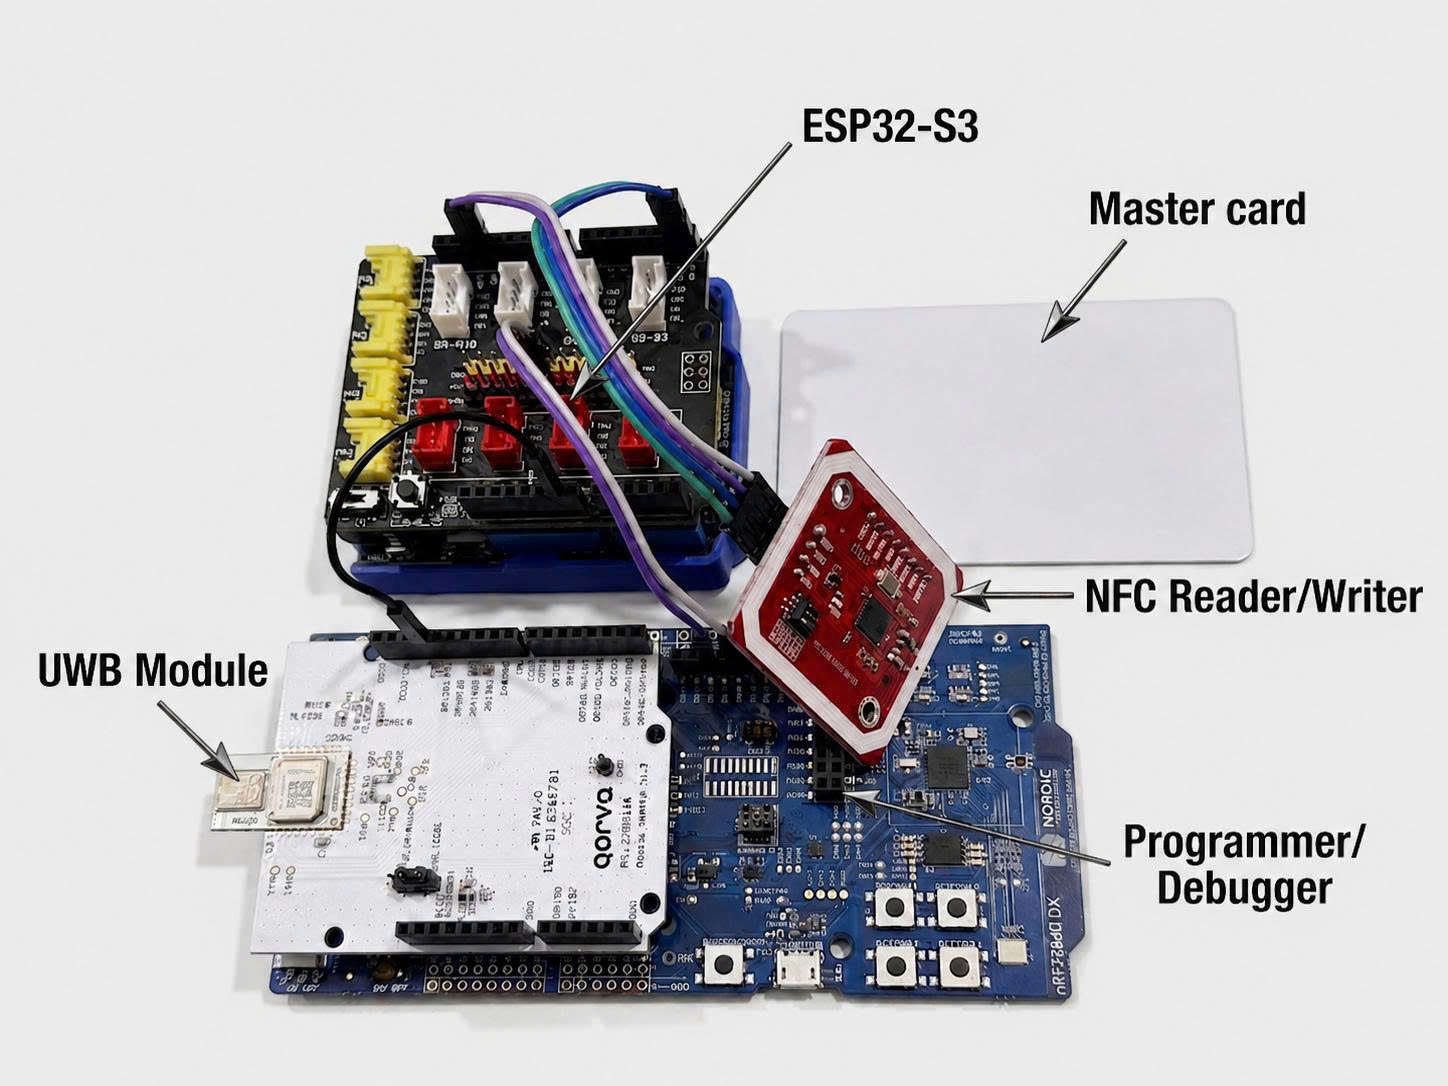
\includegraphics[width=0.8\textwidth]{image/section5/hardware.jpg} 
    \caption[Sơ đồ ghép nối hệ thống UWB đa mỏ neo]{Sơ đồ ghép nối hệ thống UWB đa mỏ neo: ESP32-S3 (trung tâm), ba mỏ neo DWM3001CDK, cầu nối PC và điện thoại Controller. \textit{(Sinh viên lưu ý cập nhật hình minh họa cho đúng cấu trúc liên kết mới.)}}
    \label{fig:uwb_hardware_arch}
\end{figure}


Sự kết hợp giữa ESP32-S3 (chuyên xử lý ứng dụng và hợp nhất dữ liệu) với ba mỏ neo DW3000 (chuyên xử lý tín hiệu UWB) và cầu nối PC (chuyên thu thập/đóng gói dữ liệu) tạo ra một hệ thống nhúng có độ tin cậy cao, mang đậm tính thực tiễn và tuân thủ chặt chẽ các thiết kế tham chiếu (Reference Design) của ngành công nghiệp ô tô hiện đại.

\begin{figure}[H]
    \centering
    \begin{minipage}{0.48\textwidth}
        \centering
        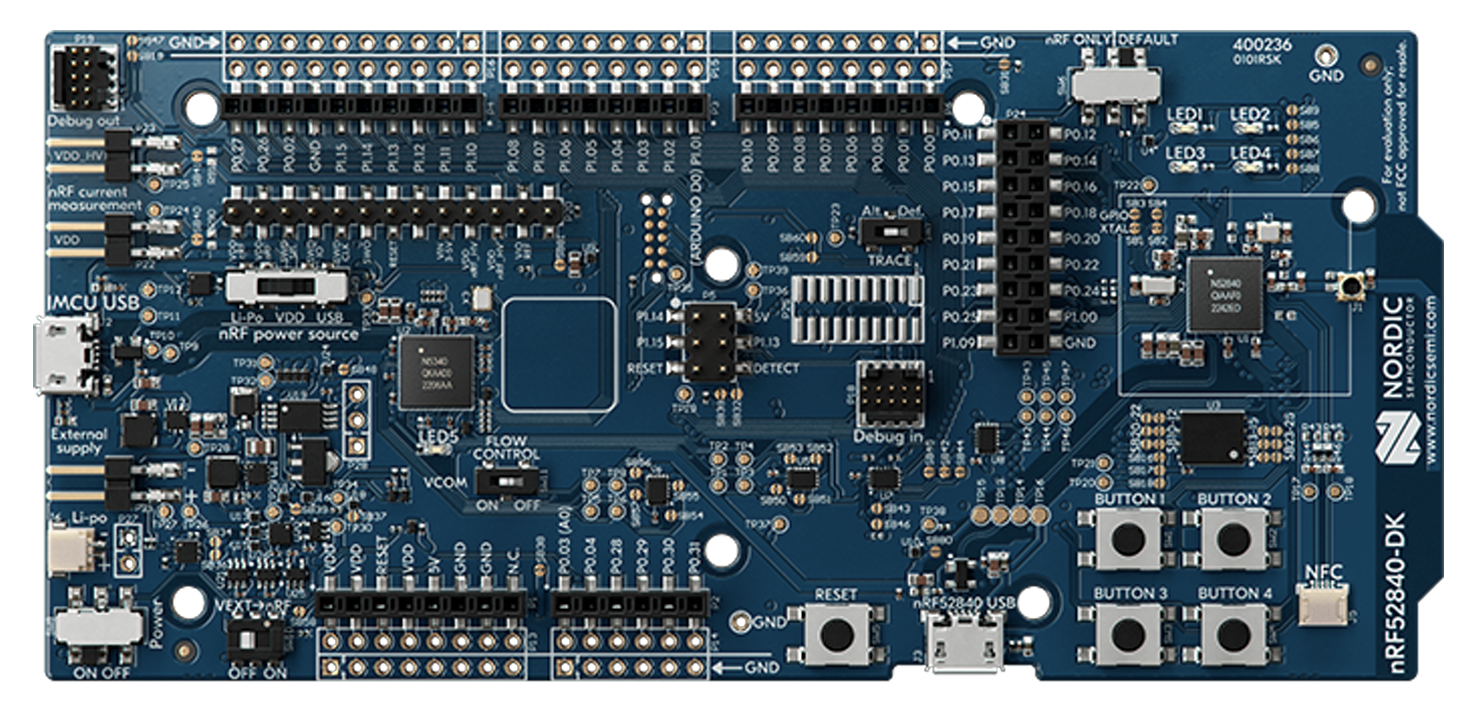
\includegraphics[width=\linewidth]{image/section5/nRF52840_DK.png}
        \caption[Mạch trung gian nRF52840]{Mạch trung gian nRF52840 (\textbf{Nguồn:} \href{https://docs.edgeimpulse.com/hardware/boards/nordic-semi-nrf52840-dk}{Nordic Semi nRF52840 DK})}
        \label{fig:hardware}
    \end{minipage}
    \hfill
    \begin{minipage}{0.48\textwidth}
        \centering
        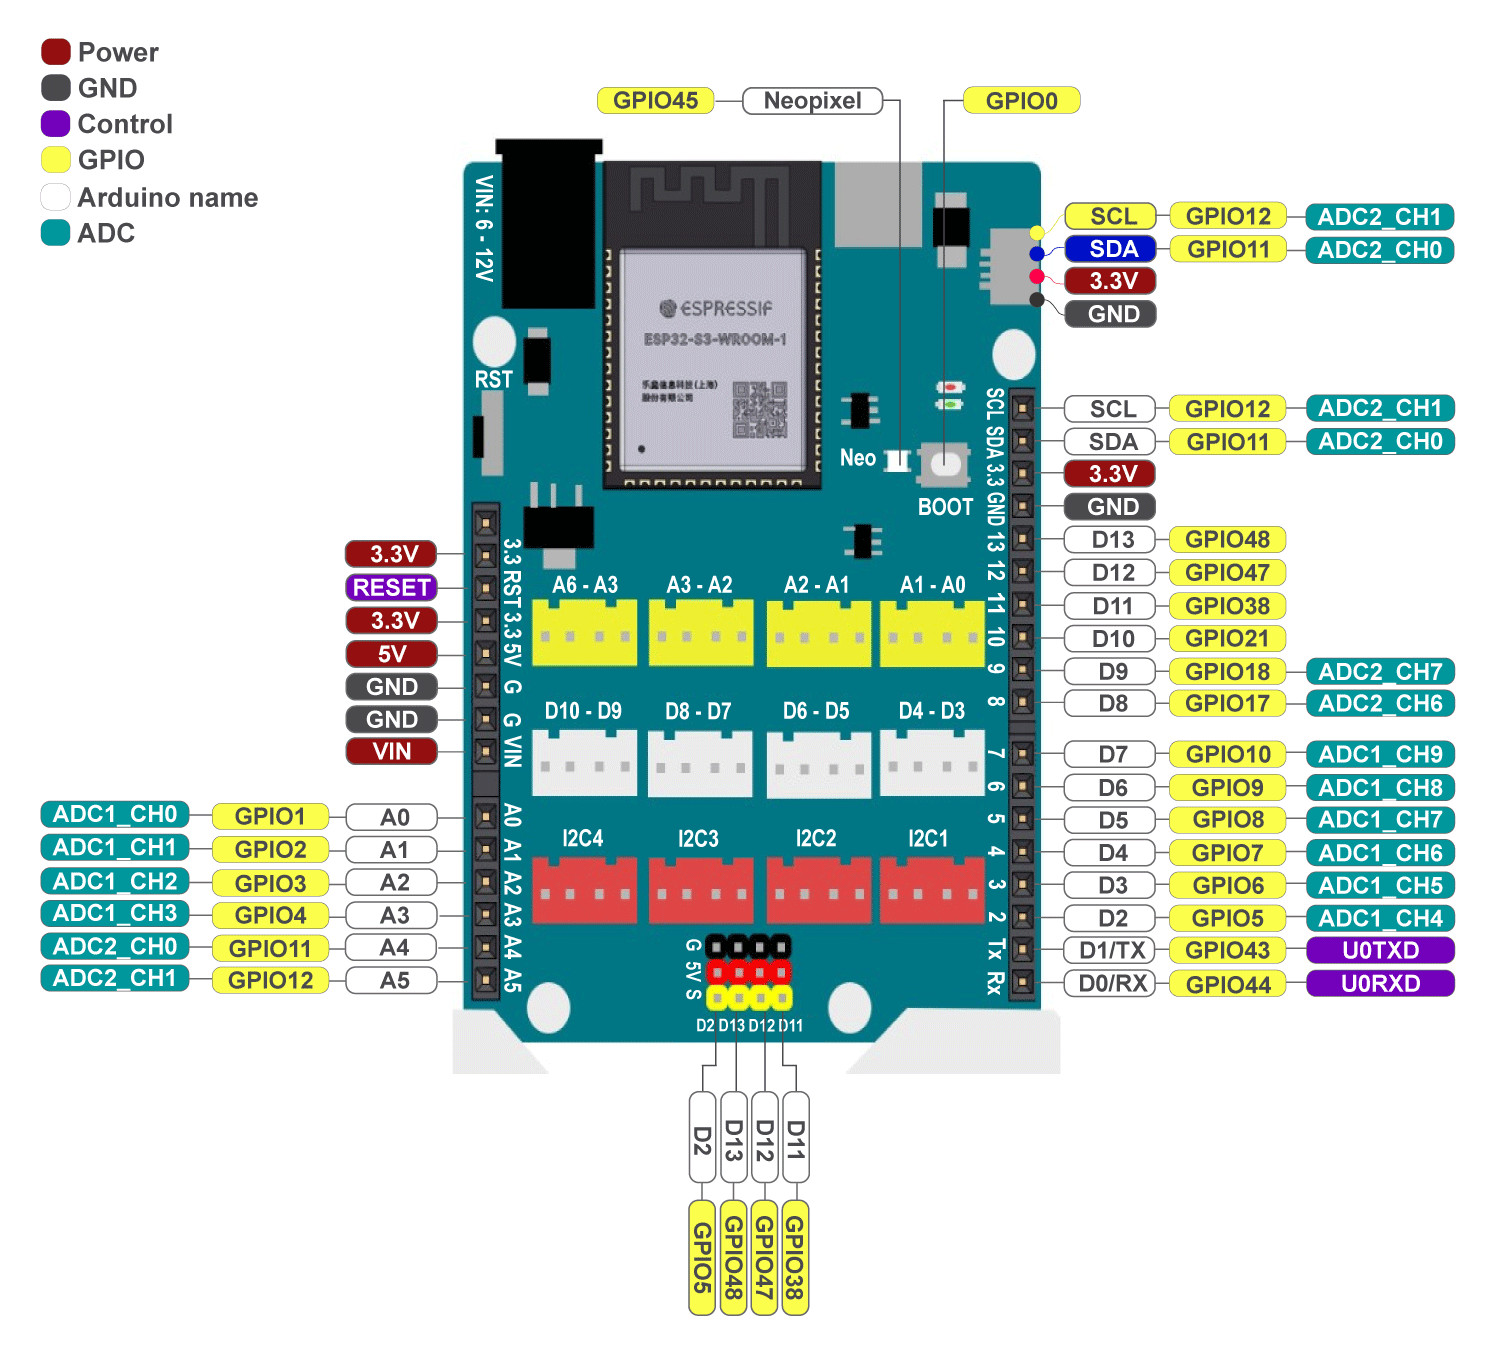
\includegraphics[width=\linewidth]{image/section5/yolouno_spec.jpg}
        \caption[Sơ đồ chân Yolo Uno ESP32-S3]{Sơ đồ chân Yolo Uno ESP32-S3 (\textbf{Nguồn:} \href{https://docs.ohstem.vn/en/latest/yolo_uno/yolo_uno_khoi_lenh/gioi_thieu_yolo_uno.html}{OhStem - Yolo UNO doc})}
        \label{fig:spec_yolouno}
    \end{minipage}
\end{figure}

\begin{figure}[H]
    \centering
    \begin{minipage}{0.38\textwidth}
        \centering
        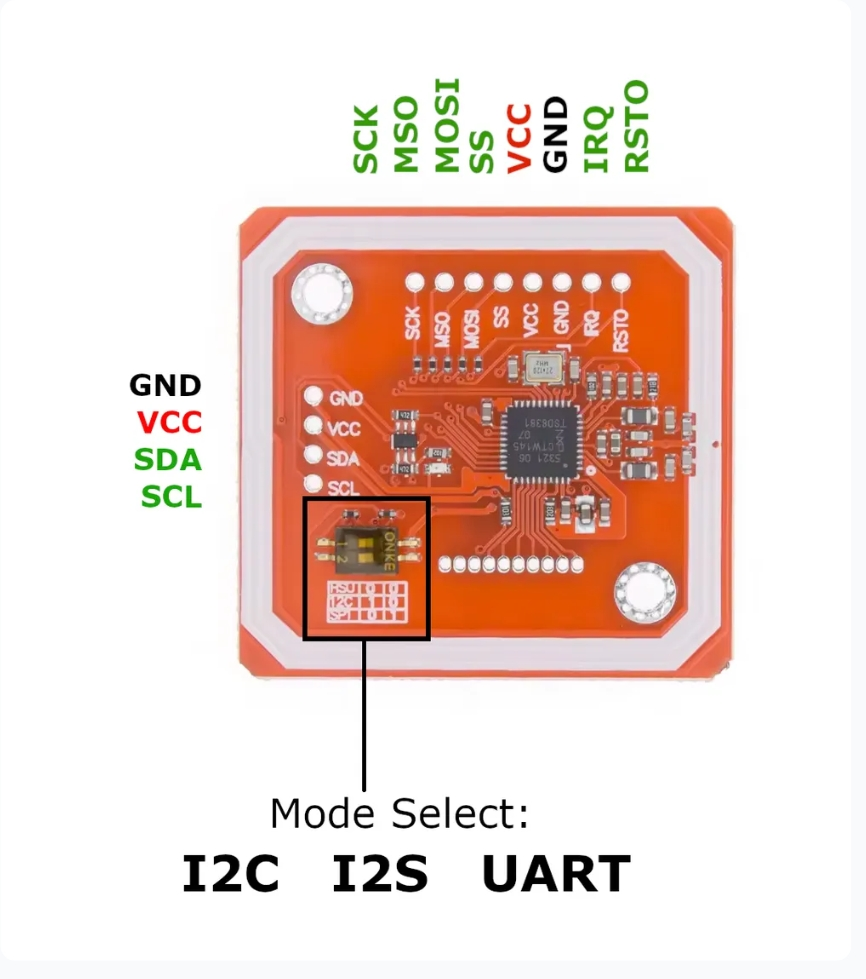
\includegraphics[width=\linewidth]{image/section5/spec_pn532.jpeg}
        \caption[Module NFC PN532]{Module NFC PN532 (\textbf{Nguồn:} \href{https://www.espboards.dev/sensors/pn532/}{ESPBoards - PN532 NFC Module Pinout})}
        \label{fig:spec_pn532}
    \end{minipage}
    \hfill
    \begin{minipage}{0.38\textwidth}
        \centering
        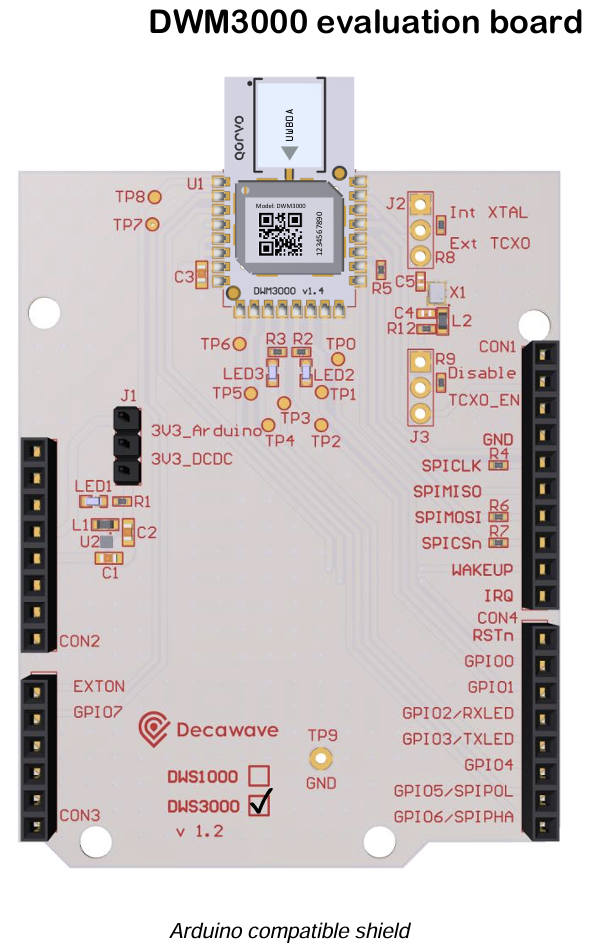
\includegraphics[width=\linewidth]{image/section5/DWM3000EVB.png} % Cập nhật tên file ảnh DWM3000EVB nếu cần
        \caption[Module UWB DWM3000EVB]{Module UWB DWM3000EVB (\textbf{Nguồn:} \href{https://www.digikey.tw/en/products/detail/qorvo/DWM3000EVB/24367408}{DWM3000EVB Qorvo - DigiKey})}
        \label{fig:spec_dwm3000}
    \end{minipage}
    \hfill
    \begin{minipage}{0.38\textwidth}
        \centering
        \includegraphics[width=\linewidth]{image/section5/DWM3001CDK.jpg} % Cập nhật tên file ảnh mỏ neo UWB nếu cần
        \caption[Mỏ neo UWB DWM3001CDK (vi mạch DW3000)]{Mỏ neo UWB DWM3001CDK (vi mạch Qorvo DW3000) (\textbf{Nguồn:} \href{https://www.qorvo.com/products/p/DWM3001CDK}{DWM3001CDK Qorvo})}
        \label{fig:spec_dwm3001cdk}
    \end{minipage}
\end{figure}








%------------------------------------------------------------------------------------






\subsection{Hiện thực phần mềm}

Kiến trúc phần mềm trên ESP32 được xây dựng trên nền tảng hệ điều hành thời gian thực FreeRTOS, cho phép các tác vụ (NFC, BLE, UWB) hoạt động đa luồng (Multi-tasking) một cách mượt mà.

\subsection{Máy trạng thái hữu hạn xuyên tầng (Cross-layer FSM)}

Cốt lõi điều khiển của ESP32 là Máy trạng thái hữu hạn (FSM) quản lý toàn bộ vòng đời truy cập. Lớp \texttt{FSMIntegration} đóng vai trò Adapter, nhận sự kiện từ các module phần cứng và điều hướng FSM.

\begin{itemize}
    \item \textbf{Khởi tạo (INIT \& IDLE):} Hệ thống duy trì quảng bá BLE và chờ quét thẻ NFC.
    \item \textbf{Cấp quyền (PROVISIONING - Phase A):} Điều khiển luồng APDU với điện thoại qua module PN532. Lưu trữ định danh điện thoại vào NVS.
    \item \textbf{Xác thực (AUTH - Phase B):} Quản lý tiến trình bắt tay mật mã (ECDH, HKDF) qua kết nối BLE. Khi hoàn tất, hệ thống đạt trạng thái \texttt{AUTH\_SECURE\_CHANNEL\_READY}.
    \item \textbf{Đo khoảng cách và Mở khóa (RANGING \& UNLOCK - Phase C \& D):} Khi nhận OOB Payload qua BLE, FSM cho phép luồng UWB Ranging hoạt động. Trạng thái \texttt{UNLOCKING\_EXECUTE} chỉ được kích hoạt khi cả kênh BLE và dữ liệu UWB đều hợp lệ.
\end{itemize}

\subsection{Xử lý NFC và Provisioning (Phase A)}
Module \texttt{nfc\_session.cpp} (chạy trên \texttt{NFCTask}) chịu trách nhiệm thiết lập kênh tin cậy ban đầu (Trust Establishment). Để khắc phục hiện tượng nhiễu tín hiệu RF, hệ thống áp dụng kỹ thuật \textit{Adaptive Polling} (chống rung tín hiệu): yêu cầu xác nhận sự hiện diện ổn định của thẻ qua nhiều chu kỳ đọc liên tiếp (\texttt{stableReads}) trước khi thiết lập kết nối APDU.

\noindent\begin{minipage}{\linewidth}
\begin{lstlisting}[language=C++, caption={Adaptive Polling logic cho NFC}]
bool waitForCard(uint32_t timeoutMs = 15000, uint8_t stableReads = 2) {
    while (true) {
        // Debounce logic: Request for successive stability detection
        if (nfc->inListPassiveTarget()) {
            if (++stableCount >= stableReads) return true;
        } else {
            stableCount = 0; // Reset if signal is lost.
        }
    }
}
\end{lstlisting}
\end{minipage}

Quy trình APDU bao gồm: Lựa chọn Applet (\texttt{SELECT AID}), trao đổi thông tin định danh, xác thực chữ ký số bằng thuật toán ECDSA. Nếu thành công, thiết bị sẽ được lưu vào danh sách truy cập (NVS).

\subsection{Giao thức xác thực BLE (Phase B)}
Giai đoạn này thiết lập kênh truyền an toàn không dây. Để tránh gây nghẽn (timeout) cho kết nối BLE do các phép toán mật mã đường cong Elliptic tốn nhiều tài nguyên, hệ thống tách các phép toán này vào một FreeRTOS Task độc lập (\texttt{AuthWorker}). Quy trình mật mã tuân thủ cấu trúc ECDH Ephemeral:

\noindent\begin{minipage}{\linewidth}
\begin{lstlisting}[language=C++, caption={Các bước mật mã chính trong Phase B}]
// 1. Generate Ephemeral P-256 (Forward Secrecy) key pair
mbedtls_ecp_gen_keypair(&grp, &d, &Q, rng, &ctr_drbg);

// 2. Calculating Shared Secrets (ECDH)
mbedtls_ecdh_compute_shared(&grp, &z, &Qp, &d, rng, &ctr_drbg);

// 3. Derive Session Keys using HKDF-SHA256
mbedtls_hkdf(md_info, salt, saltLen, ikm, ikmLen, info, infoLen, output, 32);
\end{lstlisting}
\end{minipage}

Hàm HKDF sẽ tách Shared Secret thành hai khóa độc lập: Session Encryption Key (để mã hóa AES-GCM) và Session MAC Key (để xác thực HMAC).

\subsection{Đo khoảng cách đa mỏ neo và Định vị Trilateration (Phase C)}
Đây là trọng tâm vật lý của hệ thống. Sau khi xác thực BLE (Phase B), điện thoại gửi lệnh \texttt{RANGING\_START} qua đường hầm CCC. ESP32 (lớp \texttt{UwbBridge}) chuyển thành lệnh \texttt{CMD:START\_RANGING} gửi sang cầu nối PC, cầu nối này khởi tạo phiên DS-TWR multicast trên ba mỏ neo.

Trong mỗi vòng đo, điện thoại (Controller) trao đổi xung với cả ba mỏ neo (Responder) theo giao thức \textbf{Symmetrical Double-Sided Two-Way Ranging (DS-TWR)}. Cầu nối PC thu thập ba khoảng cách $d_0, d_1, d_2$, kiểm tra tính tươi (freshness) và phạm vi hợp lệ $[0.1,\,30]$ m, rồi đóng gói thành một dòng văn bản gửi sang ESP32 qua USB-CDC:

\noindent\begin{minipage}{\linewidth}
\begin{lstlisting}[language=C++, caption={Khung dữ liệu RANGE và hàm phân tích trên ESP32}]
// Frame received from PC bridge over USB-CDC:
//   RANGE:d0=1.82,d1=0.97,d2=3.14,valid=1
bool UwbBridge::parseRange(const char* line, RangingFrame& frame) {
    double d0, d1, d2; int valid;
    if (sscanf(line, "RANGE:d0=%lf,d1=%lf,d2=%lf,valid=%d",
               &d0, &d1, &d2, &valid) != 4) return false;
    frame.d[0] = d0; frame.d[1] = d1; frame.d[2] = d2;
    frame.valid_mask = valid ? 0x07 : 0x00;   // 0b111 when all three are valid
    frame.t_ms = millis();
    return true;
}
\end{lstlisting}
\end{minipage}

Cờ \texttt{valid} chỉ được bật khi \textbf{cả ba} khoảng cách đều tươi và nằm trong phạm vi hợp lệ. Khi đủ điều kiện, ESP32 tiến hành định vị hai bước: \texttt{Trilateration::solve} trả về tọa độ $(x, y)$ kèm chất lượng lời giải RMS, sau đó \texttt{Ekf::update} hợp nhất phép đo vào quỹ đạo:

\noindent\begin{minipage}{\linewidth}
\begin{lstlisting}[language=C++, caption={Định vị Trilateration và cập nhật EKF}]
// 1. Trilateration: 3 khoang cach -> toa do (x, y) + chat luong RMS
Trilateration::Result fix = Trilateration::solve(frame.d, frame.valid_mask);

// 2. EKF: cap nhat vi tri, uoc luong van toc (x, y, vx, vy)
if (fix.valid) {
    double sigma = clamp(fix.rms, 0.05, 1.0);   // nhieu do ~ chat luong loi giai
    ekf.update(fix.x, fix.y, frame.t_ms, sigma);
}
ekf.predictTo(millis());   // du bao bu khi mat khung du lieu
\end{lstlisting}
\end{minipage}

Bộ lọc Kalman hai chiều chạy ở nhịp cố định 10 Hz, độc lập với nhịp nhận khung dữ liệu, và tự động dự báo bù khi một vài khung bị mất (tối đa 2 giây).

\subsection{Quyết định truy cập theo vùng hình học (Phase D)}

Sau khi bộ lọc Kalman hai chiều cung cấp trạng thái mượt $(x, y, v_x, v_y)$ ở nhịp 10 Hz, hệ thống thực hiện \textbf{phân vùng không gian} (Geofencing) và ra quyết định truy cập thông qua một \textbf{máy trạng thái truy cập} gồm ba trạng thái. Đây là tầng lõi tất định (deterministic) của hệ thống, hoạt động độc lập với tầng học sâu, đảm bảo tính an toàn cơ học (fail-safe) ngay cả khi tầng AI chưa sẵn sàng.

\subsubsection{Phân vùng không gian (Geofencing)}

Module \texttt{Geofence} ánh xạ tọa độ đã lọc $(x, y)$ vào bốn vùng ảo trong hệ quy chiếu gắn với xe (gốc tọa độ tại tâm xe, $+x$ hướng sang phải, $+y$ hướng về phía trước):

\begin{itemize}
    \item \textbf{DRIVER\_SEAT:} vùng ghế lái, tâm $(-0.35,\,0)$ bán kính $0.45$ m --- đại diện vị trí người dùng ngồi vào xe.
    \item \textbf{DRIVER\_DOOR:} vùng cửa tài xế, tâm $(-0.95,\,0)$ bán kính $2.0$ m (trùng với mỏ neo $A_2$ --- cột B bên trái).
    \item \textbf{WELCOME:} vùng chào đón, bán kính $4.0$ m tính từ tâm xe.
    \item \textbf{OUTSIDE:} bên ngoài vùng chào đón.
\end{itemize}

Bộ lọc \texttt{Hysteresis} chỉ chấp nhận vùng ổn định (đồng nhất trong 3 chu kỳ liên tiếp) nhằm triệt tiêu hiện tượng chuyển vùng liên tục tại biên giới (boundary chatter).

\subsubsection{Máy trạng thái truy cập (Access State Machine)}

Module \texttt{AccessController} duy trì ba trạng thái hoạt động:

\begin{itemize}
    \item \textbf{LOCKED:} cửa khóa, chưa cấp quyền khởi động.
    \item \textbf{DOOR\_UNLOCKED:} cửa đã mở, người dùng chưa ngồi vào ghế lái.
    \item \textbf{OCCUPIED:} người dùng đã ngồi vào ghế lái --- cửa khóa lại và cấp quyền khởi động động cơ.
\end{itemize}

Các chuyển trạng thái được điều khiển bởi các cổng tất định:

\begin{enumerate}
    \item \textbf{Mở khóa} (\texttt{LOCKED $\rightarrow$ DOOR\_UNLOCKED}): chỉ khi người dùng ở vùng cửa (\texttt{DRIVER\_DOOR}/\texttt{DRIVER\_SEAT}), \textbf{giảm tốc gần như dừng hẳn} (tốc độ $< 0.4$ m/s) trong 3 chu kỳ liên tiếp, đồng thời không có chuyển động rời xa (cổng vận tốc hướng tâm).
    \item \textbf{Định cư ghế lái} (\texttt{DOOR\_UNLOCKED $\rightarrow$ OCCUPIED}): khi người dùng đứng yên trong vùng \texttt{DRIVER\_SEAT} liên tục 3 giây. Lúc này hệ thống khóa cửa và cấp quyền khởi động (chân \texttt{GPIO27}).
    \item \textbf{Rời đi} (\texttt{OCCUPIED $\rightarrow$ LOCKED}): khi người dùng ra khỏi vùng chào đón (\texttt{OUTSIDE}) và có vận tốc hướng ra xa trong 3 chu kỳ liên tiếp. Hệ thống thu hồi quyền khởi động và khóa cửa.
    \item \textbf{Hủy bỏ} (\texttt{DOOR\_UNLOCKED $\rightarrow$ LOCKED}): người dùng bỏ đi mà không ngồi vào ghế --- hệ thống khóa cửa trở lại.
\end{enumerate}

Trong đó, \textbf{cổng giảm tốc} (deceleration gate) là bổ sung quan trọng: yêu cầu người dùng phải giảm tốc gần như dừng hẳn ở gần cửa mới được mở khóa, nhờ đó loại bỏ triệt để các trường hợp người dùng chỉ \textit{đi ngang qua} cửa (tangential pass) mà không có ý định vào xe --- điều mà một ngưỡng vận tốc hướng tâm đơn thuần không thể phân biệt được.

\noindent\begin{minipage}{\linewidth}
\begin{lstlisting}[language=C++, caption={Máy trạng thái truy cập (AccessController) rút gọn}]
void AccessController::handlePosition(double x, double y,
                                      double vx, double vy) {
  double vr = radialSpeed(x, y, vx, vy);          // >0 roi xa, <0 tien lai
  Zone  z  = zone_hyst.update(x, y, 3);           // vung on dinh (debounce 3)
  bool movingAway = (vr > 0.10);
  double speed = hypot(vx, vy);

  switch (state_) {
    case LOCKED:
      if (z == OUTSIDE || movingAway) { hits = 0; return; }
      if ((z == DRIVER_DOOR || z == DRIVER_SEAT) && speed < 0.4) {
        if (++hits >= 3) { fireUnlock(); state_ = DOOR_UNLOCKED; hits = 0; }
      } else hits = 0;
      break;
    case DOOR_UNLOCKED:
      if (z == DRIVER_SEAT && speed < 0.4) {       // ngoi yen ghe lai 3s
        if (settledFor(3s)) { lockDoor(); setIgnition(true); state_ = OCCUPIED; }
      }
      if (z == OUTSIDE && movingAway) { lockDoor(); state_ = LOCKED; }
      break;
    case OCCUPIED:
      if (z == OUTSIDE && movingAway) {            // roi di
        if (++leaveHits >= 3) { setIgnition(false); lockDoor(); state_ = LOCKED; }
      } else leaveHits = 0;
      break;
  }
}
\end{lstlisting}
\end{minipage}

\subsubsection{Kích hoạt cơ cấu chấp hành}

Kết quả ra quyết định được phản ánh qua hai kênh tín hiệu:

\begin{itemize}
    \item \textbf{Chân \texttt{GPIO26}}: điều khiển rơ-le khóa/mở cửa --- mức \texttt{LOW} tương ứng trạng thái khóa, xung \texttt{HIGH} trong 500 ms tương ứng lệnh mở cửa.
    \item \textbf{Chân \texttt{GPIO27}}: tín hiệu cấp quyền khởi động động cơ --- mức \texttt{HIGH} khi ở trạng thái \texttt{OCCUPIED}.
\end{itemize}

Toàn bộ quy trình chuyển trạng thái được ghi nhận qua các thẻ log \texttt{[ZONE]}, \texttt{[STATE]} và \texttt{[IGNITION]} phục vụ giám sát và kiểm thử. Logic tất định này tạo ra trải nghiệm \textit{Passive Keyless Entry} mượt mà: mở cửa khi người dùng tiến lại gần và dừng lại, khóa cửa và cấp quyền khởi động khi người dùng đã định cư ghế lái, rồi khóa xe và thu hồi quyền khi người dùng rời đi.






%------------------------------------------------------------------------------------






\section{Triển khai phần ứng dụng di động}

Mặc dù Flutter được sử dụng làm framework phát triển chính, nhưng đối với một hệ thống yêu cầu bảo mật phần cứng nghiêm ngặt như Smart Car Access (chuẩn CCC), ứng dụng được thiết kế theo kiến trúc phân tầng sâu. Flutter chỉ đóng vai trò là Lớp Giao diện (Presentation) và Điều phối logic (Domain), trong khi toàn bộ các tác vụ mật mã và điều khiển phần cứng vô tuyến được chuyển giao (delegate) xuống tầng Native Android (Kotlin).

\subsection{Tích hợp Native Android}
Ứng dụng thiết lập một hệ thống \texttt{MethodChannel} và \texttt{EventChannel} để ánh xạ trực tiếp các lệnh từ Dart xuống API hệ thống của Android:

\begin{itemize}
    \item \textbf{Kênh \texttt{smartcar/keystore}:} Chịu trách nhiệm quản lý định danh. Native Kotlin (\texttt{KeystoreBridge.kt}) trực tiếp sinh cặp khóa ECDSA P-256 và bảo vệ Private Key vĩnh viễn trong vùng an toàn (Hardware-backed) của Android Keystore. Các thao tác ký điện tử ở Phase A được thực hiện tại đây để khóa bí mật không bao giờ lọt lên tầng Flutter.
    \item \textbf{Kênh \texttt{smartcar/mastercard} \& \texttt{smartcar/nfc\_reader}:} Quản lý phiên cấp quyền (Provisioning Session). Module \texttt{MasterCardSession} nhận dữ liệu xác thực từ Flutter và giữ phiên làm việc tạm thời trong RAM để cấp phép cho tiến trình mô phỏng thẻ HCE hoạt động.
    \item \textbf{Kênh \texttt{smartcar/uwb}:} Lớp \texttt{UwbRangingBridge.kt} gọi trực tiếp API \texttt{androidx.core.uwb} của hệ điều hành, cấu hình các tham số Ranging chuẩn FiRa (Channel, Preamble Index, MAC) và sử dụng Coroutine để duy trì vòng lặp đo khoảng cách liên tục, đẩy dữ liệu tọa độ về Flutter qua luồng sự kiện.
\end{itemize}

\subsection{Cấp quyền vật lý qua Thẻ chủ (Phase A - Master Card \& HCE)}
Luồng cấp quyền (Provisioning) được chia làm hai bước tách biệt nhằm tối đa hóa bảo mật:
\begin{enumerate}
    \item \textbf{Xác nhận chủ sở hữu (Flutter):} Người dùng sử dụng Flutter App (\texttt{Master CardProvisioningService}) để quét thẻ vật lý Master Card (chứa NDEF Payload gồm \texttt{vid} và \texttt{msk}). Dữ liệu này được đẩy xuống tầng Native thông qua MethodChannel để mở khóa phiên làm việc.
    \item \textbf{Giao tiếp APDU (Native HCE):} Ngay sau đó, dịch vụ \texttt{Provisioning HostApduService} (chạy ngầm dưới nền hệ điều hành) tiếp quản. Dịch vụ này mô phỏng thẻ thông minh (AID \texttt{F00102030405}), thực hiện cơ chế xác thực SPAKE2+ từ Master Card, trao đổi khóa và ký Challenge bằng Android Keystore, hoàn toàn độc lập với vòng đời của giao diện Flutter.
\end{enumerate}

\subsection{Cơ chế chạy ngầm và Bàn giao phần cứng}
Để hiện thực hóa tính năng "Mở khóa thụ động" (Passive Keyless Entry) mà không cần người dùng mở màn hình điện thoại, ứng dụng áp dụng kiến trúc \textit{Dual-Isolate}:

\begin{itemize}
    \item \textbf{Background Isolate:} Chạy liên tục dưới dạng Android Foreground Service (\texttt{Pke BackgroundService.dart}). Luồng này lắng nghe sóng BLE, tự động kết nối và thực hiện toàn bộ luồng mật mã ECDH (Phase B) một cách âm thầm.
    \item \textbf{Foreground Isolate:} Đảm nhiệm cấu hình chip UWB. Do các chính sách bảo mật hệ thống của Android, phần cứng UWB chỉ cho phép khởi tạo khi ứng dụng đang ở trên màn hình (Foreground).
\end{itemize}

Để giải quyết bài toán chuyển tiếp giữa hai luồng độc lập mà không làm đứt kết nối BLE (gây trễ do phải quét lại), đề tài áp dụng cơ chế \textbf{Connection Hold \& Handoff}. Luồng Background sau khi xác thực BLE thành công sẽ \textbf{không gửi lệnh ngắt kết nối}, mà phát tín hiệu đánh thức luồng Foreground. Luồng Foreground lập tức tiếp quản kết nối BLE thông qua địa chỉ MAC đã biết, vá địa chỉ UWB cục bộ vào OOB Payload, gửi cho ESP32 và bật chip UWB. Thiết kế này giúp giảm thời gian chuyển tiếp từ Phase B sang Phase C xuống dưới 400ms.

\subsection{Dữ liệu và Hệ thống cảnh báo an ninh}
Ứng dụng sử dụng Firebase Firestore (\texttt{CarService.dart}) để đồng bộ hóa trạng thái xe và khóa số theo thời gian thực. Toàn bộ các thao tác ghi dữ liệu đều được ràng buộc bảo mật với \texttt{ownerId} của Firebase Auth.

Bên cạnh đó, ứng dụng tích hợp dịch vụ thu thập tọa độ \texttt{GpsService}. Dữ liệu GPS không chỉ dùng để hiển thị mà được đóng gói thành một cấu trúc nhị phân 32-byte, mã hóa tính toàn vẹn bằng HMAC-SHA256 và gửi qua BLE. Hệ thống AI (\texttt{AnomalyDetectionService}) sẽ tổng hợp các sự kiện truy cập, phân tích yếu tố thời gian/vị trí để phát cảnh báo đẩy (Push Notification) nếu phát hiện hành vi truy cập bất thường.

\subsection{Giao diện Kiểm thử Chuyên sâu (Integration Test UIs)}
Khác với các ứng dụng thông thường, giao diện hệ thống này được thiết kế đi kèm với các công cụ kiểm thử tích hợp chuyên biệt, cho phép cô lập và đánh giá từng giao thức vô tuyến trong kiến trúc Tri-Radio. Có hai màn hình kiểm thử chính:

\begin{itemize}
    \item \textbf{Giao diện Kiểm thử Phase A/B (\texttt{TestPhaseABScreen}):} 
    Chuyên dùng để kiểm tra tính toàn vẹn của Android Keystore và luồng BLE. Màn hình này mô phỏng lại các bước của dịch vụ HCE, kiểm tra sự tồn tại của khóa Identity P-256. Trong Phase B, giao diện cho phép chọn thiết bị, thực hiện luồng bắt tay ECDH và in trực tiếp các log mật mã (Shared Secret, Session Keys, Challenge) ra màn hình Console nội bộ nhằm đối chiếu với log trên ESP32.
    
    \item \textbf{Giao diện Kiểm thử UWB (\texttt{TestUwbScreen}):} 
    Được thiết kế chuyên biệt để gỡ lỗi quá trình Ranging đa mỏ neo. Màn hình cho phép các nhà phát triển kích hoạt phiên đo (Start/Stop Ranging), gửi lệnh qua đường hầm CCC, đồng thời hiển thị trực tiếp ba khoảng cách $d_0, d_1, d_2$ và trạng thái phiên từ API Native UWB (\texttt{android.ranging}) với tần số làm mới cao.
\end{itemize}

Việc tách biệt hai màn hình kiểm thử này giúp rút ngắn đáng kể thời gian gỡ lỗi phần cứng, đồng thời cung cấp công cụ trực quan để minh chứng sự hoạt động độc lập và liền mạch của các giao thức NFC, BLE và UWB trong hệ thống.






\section{Kết quả kiểm thử thực tế}

Để đảm bảo tính đúng đắn và độ ổn định của giao thức, hệ thống tích hợp các giao diện Debug chuyên dụng, cho phép cô lập và theo dõi trạng thái của từng giai đoạn, đồng thời xuất logs chi tiết từ Console.

\leavevmode
\begin{figure}[htbp]
    \centering
    \begin{minipage}{0.25\textwidth}
        \centering
        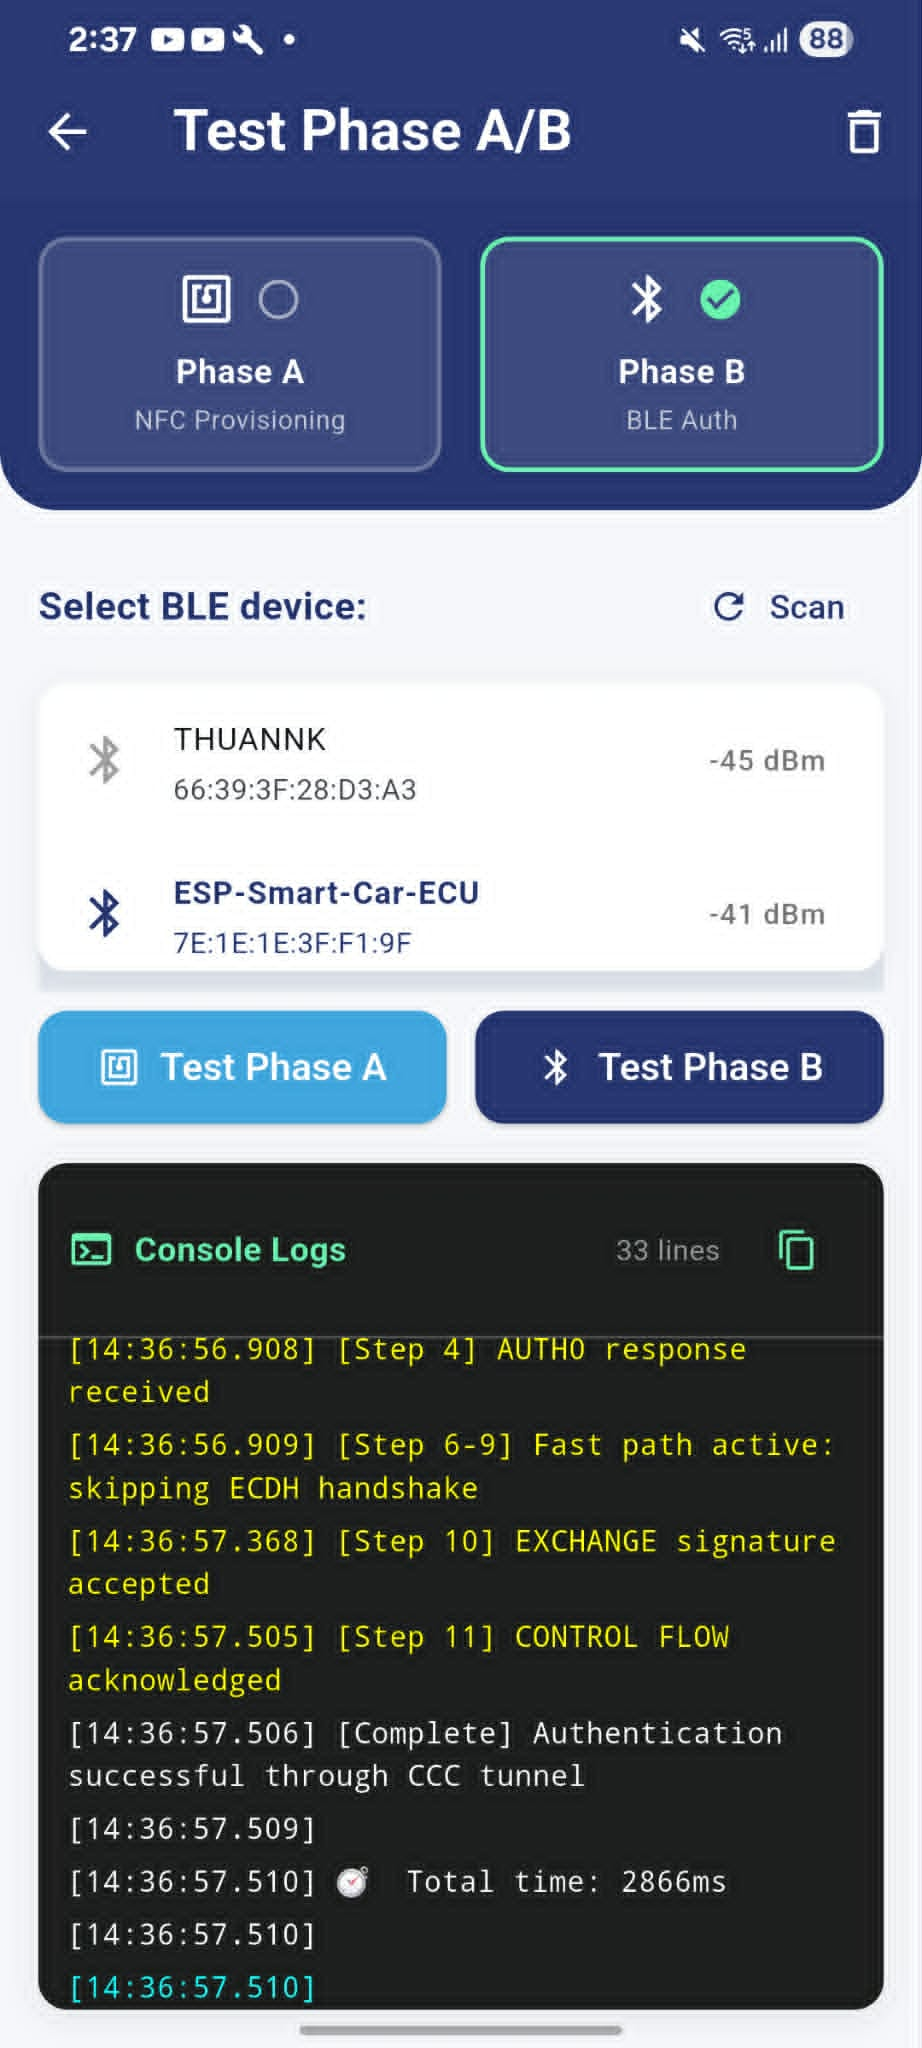
\includegraphics[width=\linewidth]{image/section5/ble_screen.jpg}
        \caption{Giao diện kiểm thử xác thực BLE (Phase B)}
        \label{fig:ble_test}
    \end{minipage}
    \hfill
    \begin{minipage}{0.25\textwidth}
        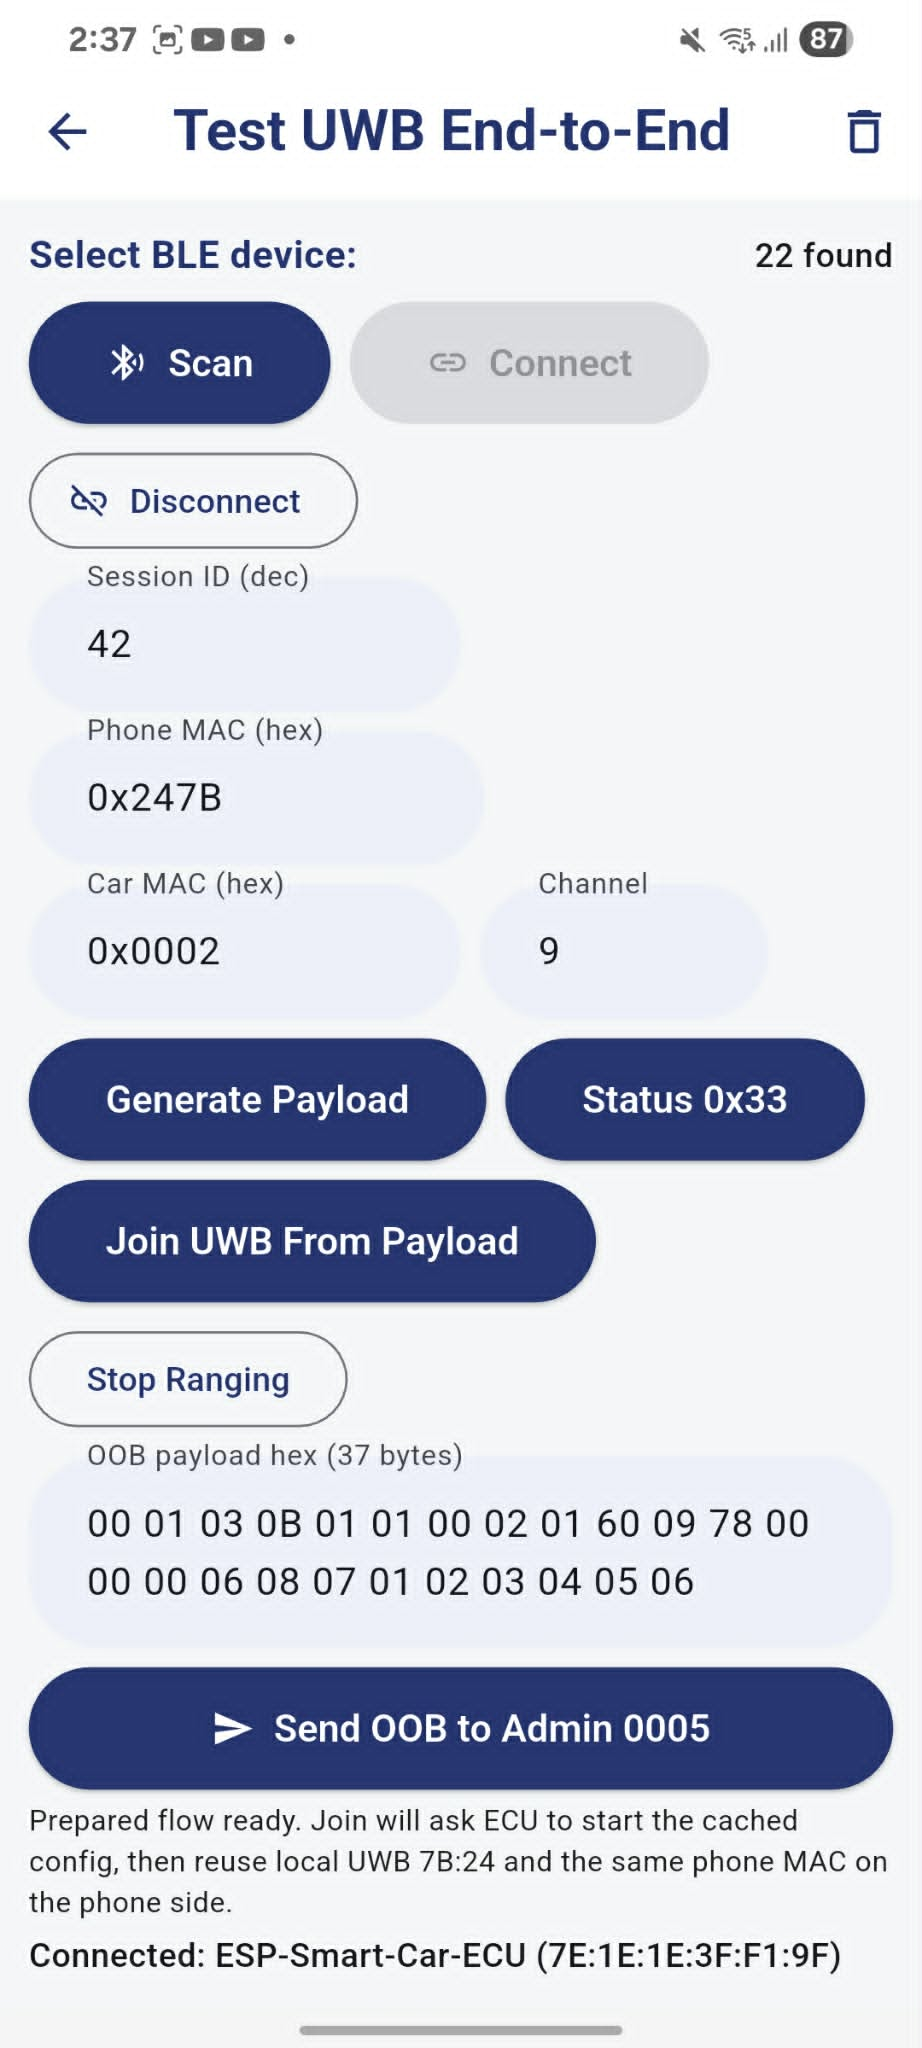
\includegraphics[width=\linewidth]{image/section5/uwb_screen_1.jpg}
        \caption{Giao diện kích hoạt UWB Ranging đa mỏ neo (Phase C) (1)}
        \label{fig:uwb_test1}
    \end{minipage}
    \hfill
    \begin{minipage}{0.25\textwidth}
        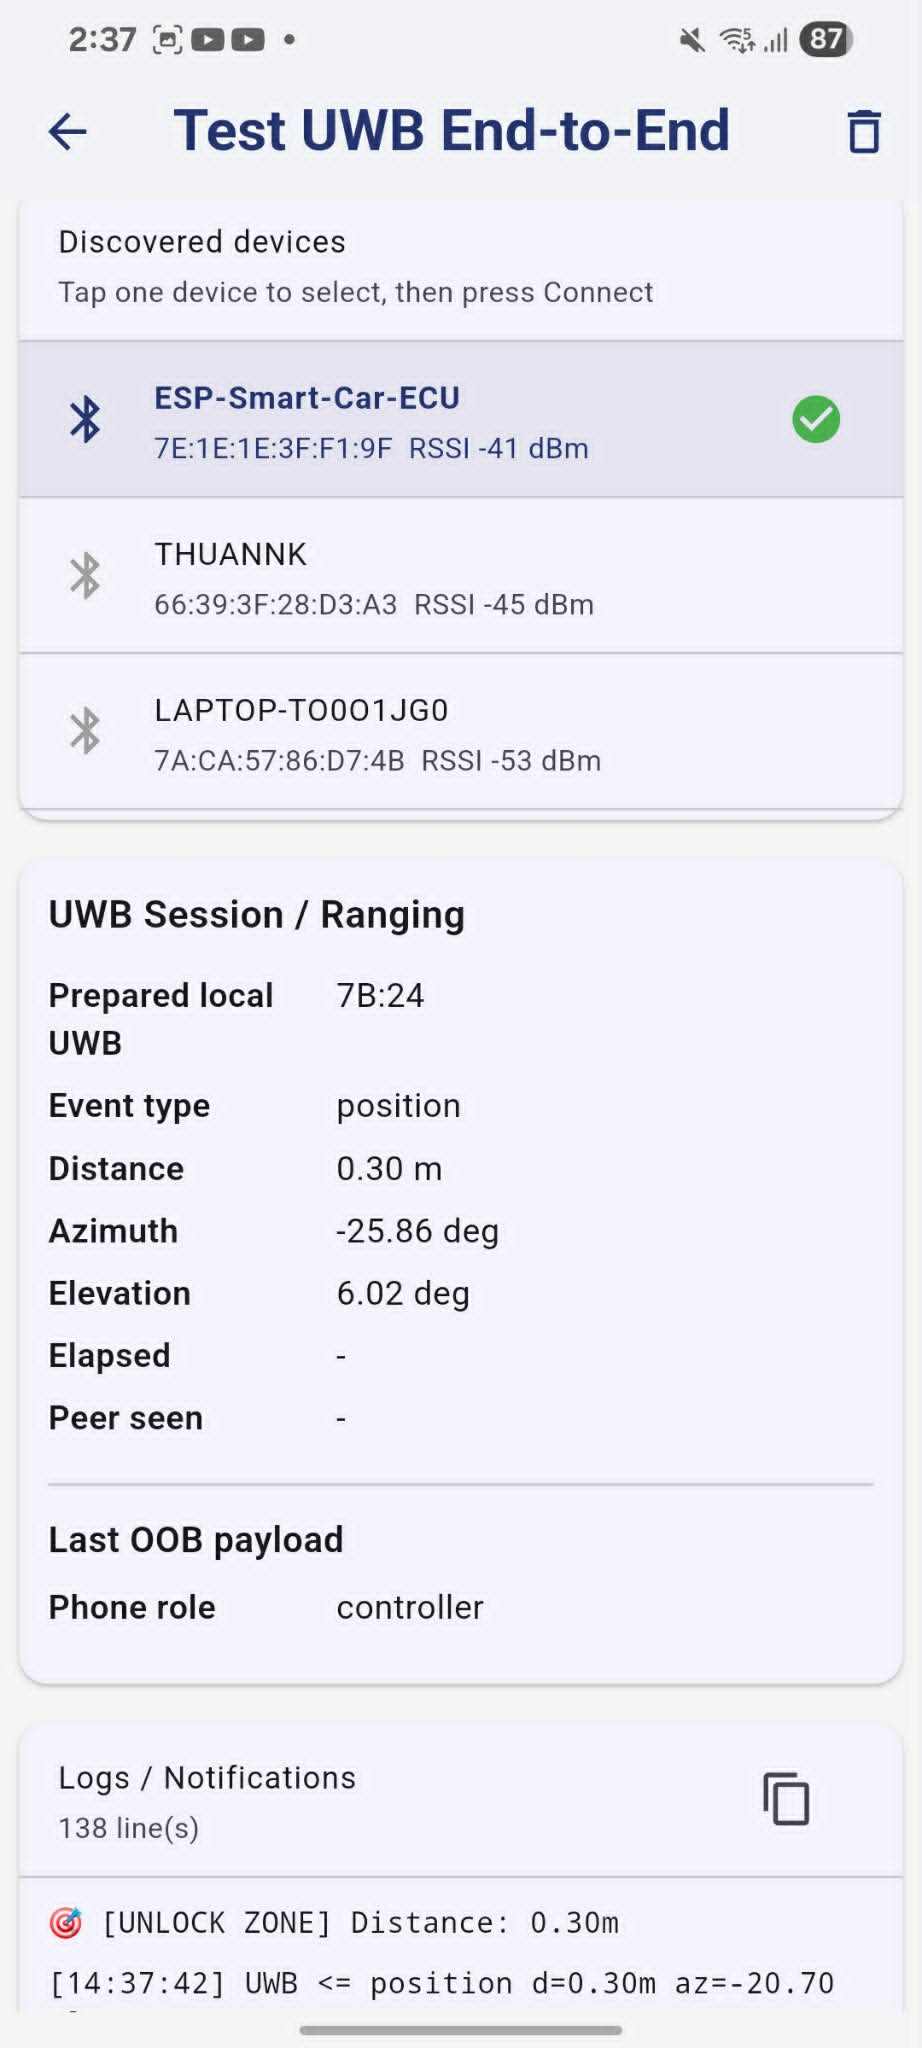
\includegraphics[width=\linewidth]{image/section5/uwb_screen_2.jpg}
        \caption{Giao diện ranging UWB Ranging (Phase C) (2)}
        \label{fig:uwb_test2}
    \end{minipage}
\end{figure}

Trong bài kiểm thử Phase B (Hình \ref{fig:ble_test}), ứng dụng tiến hành quét thiết bị BLE, thiết lập kênh an toàn và thực hiện quy trình bắt tay mật mã ECDH. Màn hình Debug hiển thị minh bạch các tham số dẫn xuất như Shared Secret và Session Keys, khẳng định kênh liên lạc đã được mã hóa an toàn.

Ngay sau khi quá trình Hand-off hoàn tất, giao diện chuyển sang bài kiểm thử Phase C (Hình \ref{fig:esp32_log}). Điện thoại thực hiện DS-TWR đồng thời với ba mỏ neo, ba khoảng cách (ví dụ: $d_0 = 1.82$m, $d_1 = 0.97$m, $d_2 = 3.14$m) được cập nhật liên tục trên màn hình, chứng minh sự đồng bộ giữa Android UWB API (\texttt{android.ranging}) và ba mỏ neo DWM3001CDK qua cầu nối PC.

\leavevmode
\begin{figure}[htbp]
	\centering
	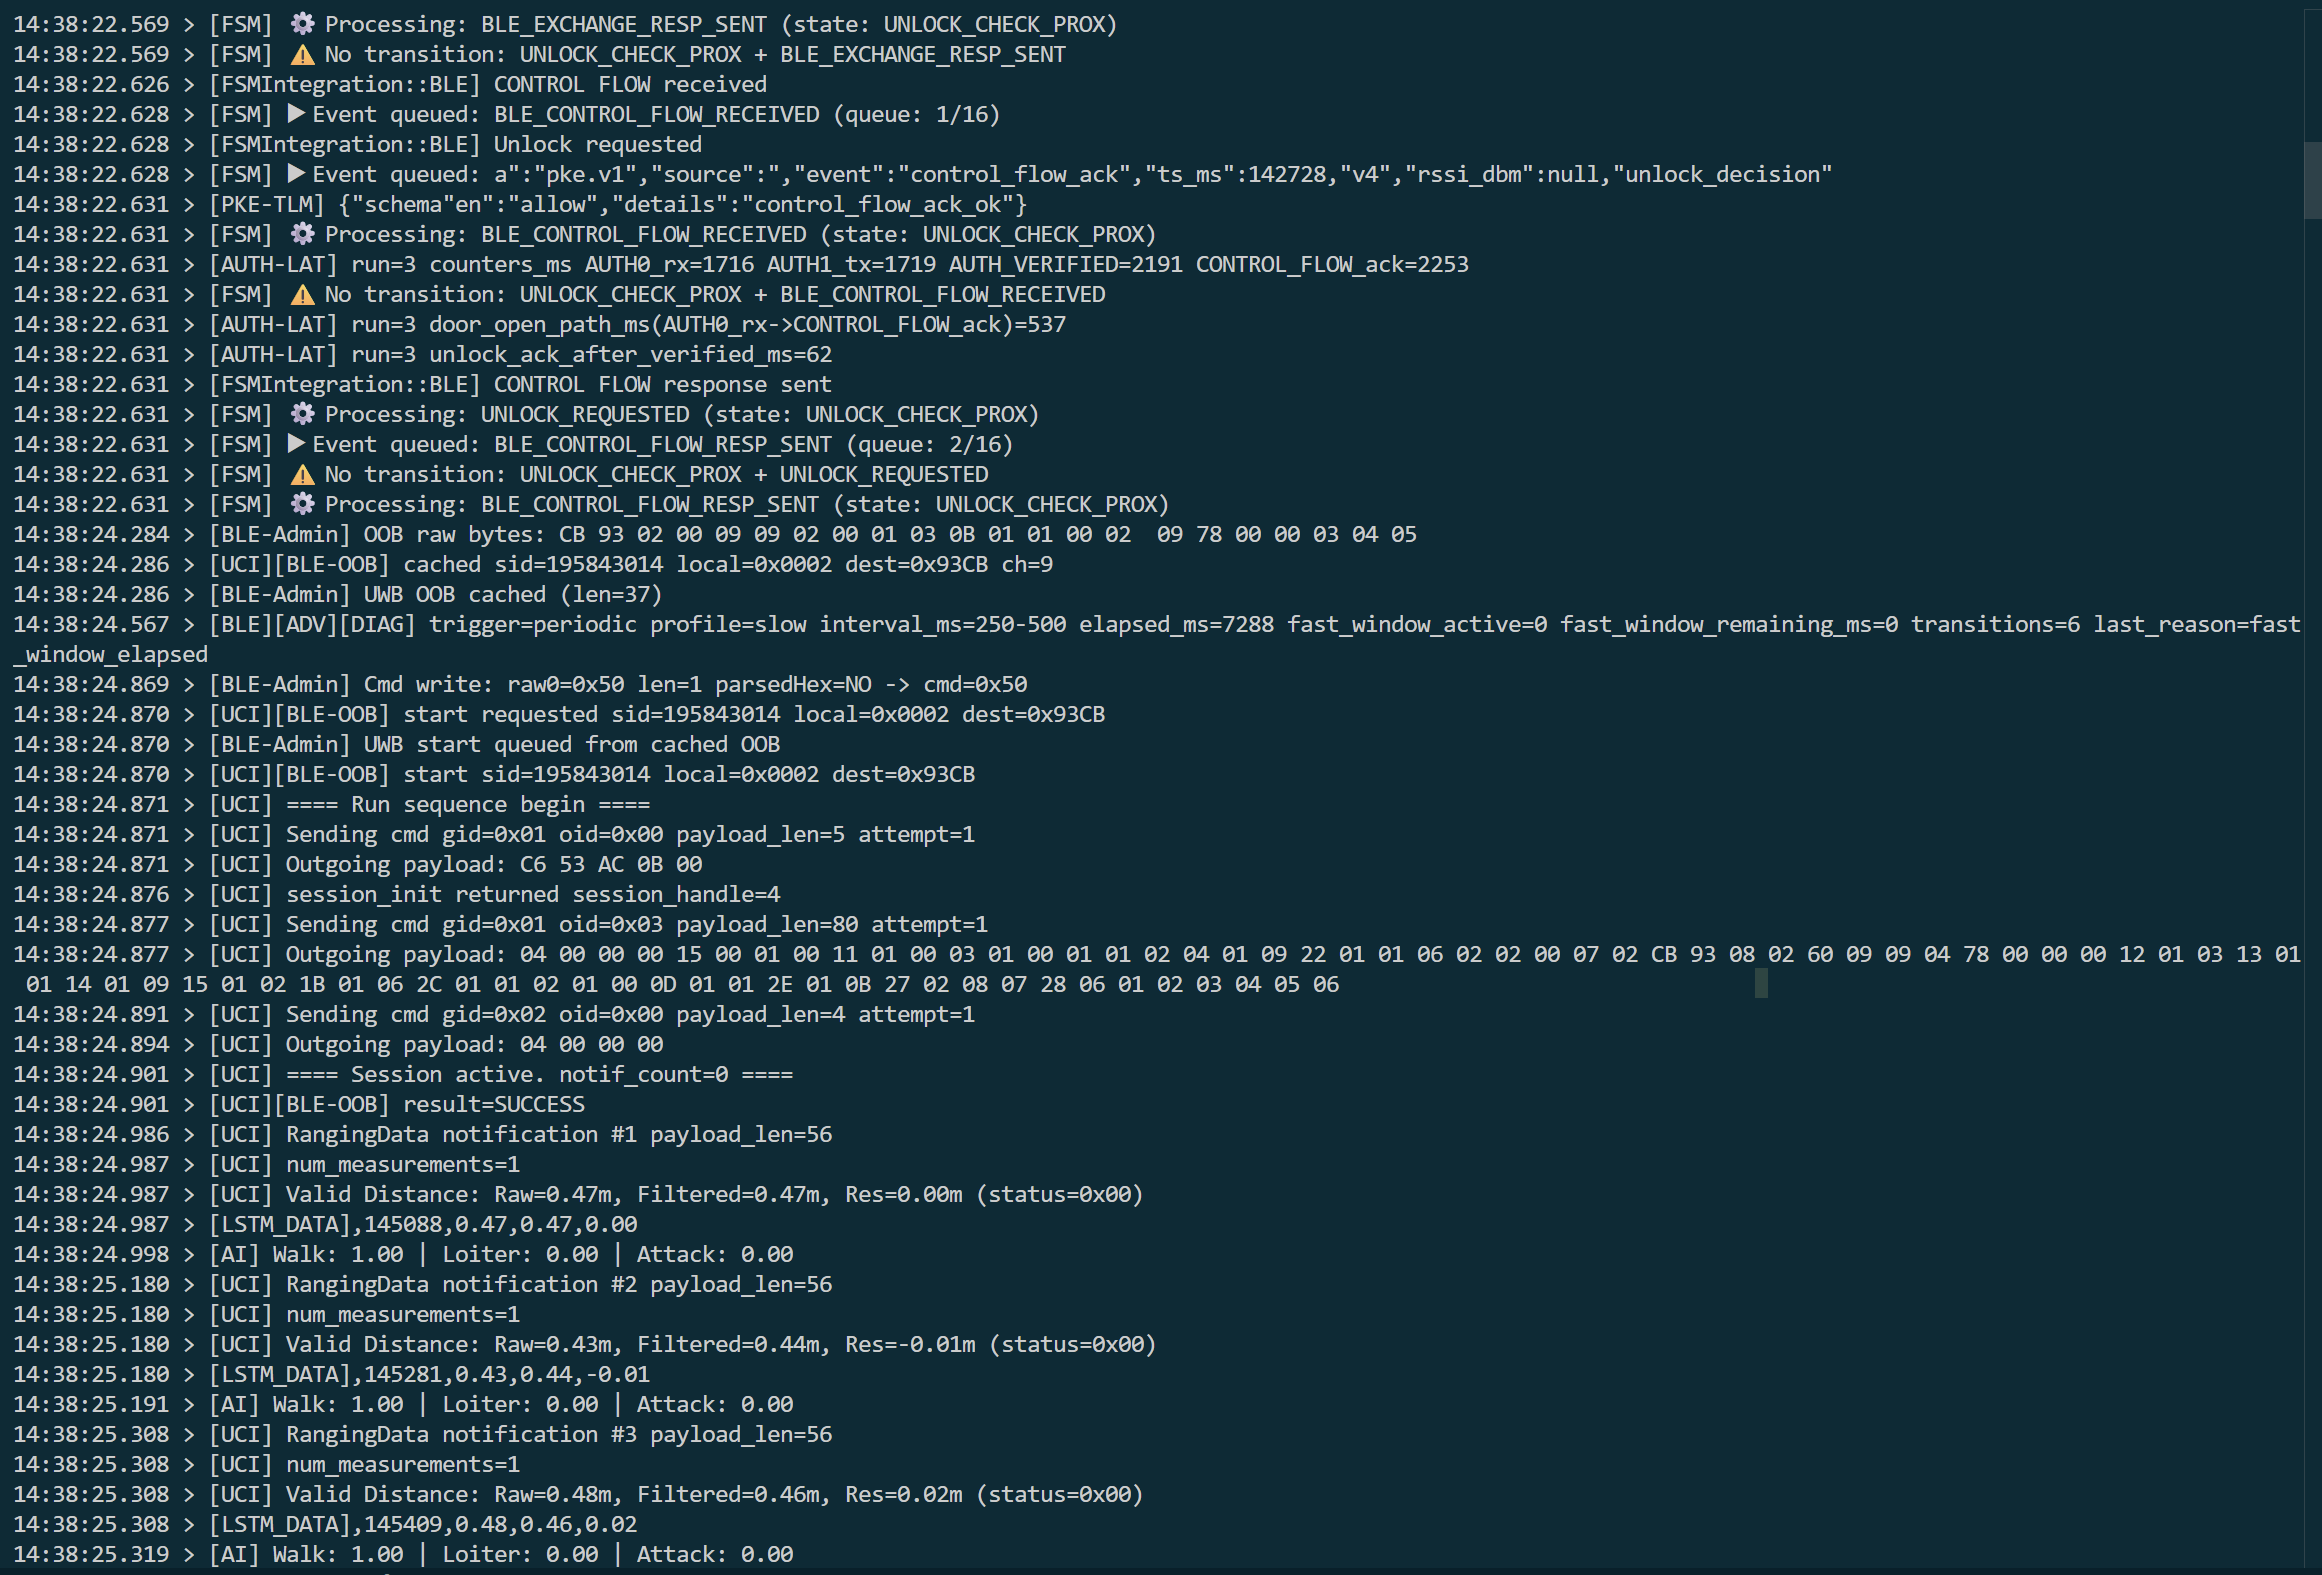
\includegraphics[width=1.0\textwidth]{image/section5/BLE TO UWB.png}
	\caption{Log xử lý xuyên tầng (BLE \& UWB) trên ESP32}
	\label{fig:esp32_log}
\end{figure}

Đối chứng từ phía vi điều khiển, log từ Serial Monitor của ESP32 (Hình \ref{fig:esp32_log}) xác nhận sự kết hợp chính xác của toàn bộ quy trình. Luồng log ghi nhận các sự kiện theo đúng thứ tự thiết kế:
\begin{enumerate}
    \item \textbf{Xác thực BLE:} Sinh khóa ephemeral, nhận Handshake, xác minh chữ ký điện thoại, tính toán ECDH và dùng HKDF sinh ra Session Keys.
    \item \textbf{Kích hoạt phiên Ranging:} Tiếp nhận lệnh \texttt{RANGING\_START} qua đường hầm CCC, ESP32 phát lệnh \texttt{CMD:START\_RANGING} sang cầu nối PC để khởi động ba mỏ neo.
    \item \textbf{Xử lý định vị thời gian thực (Trilateration + Kalman Filtering):} Ba khoảng cách thô $d_0, d_1, d_2$ từ cầu nối PC được đưa qua thuật toán Trilateration để giải tọa độ $(x, y)$, sau đó cập nhật bộ lọc Kalman hai chiều. Log hệ thống ghi nhận quá trình làm mượt quỹ đạo, triệt tiêu các xung nhiễu vật lý và ước lượng vận tốc $(v_x, v_y)$. Đây là bước tiền xử lý quan trọng để tạo ra bộ dữ liệu đầu vào ổn định cho tầng quyết định truy cập.
    \item \textbf{Suy luận ý định hành vi (On-device Inference, đang hiện thực):} Sau khi tích lũy đủ cửa sổ thời gian 25 frames, module \texttt{TrajInference} (Conv1D/TFLM) sẽ thực hiện dự báo ý định. Log Console dự kiến hiển thị các xác suất phân loại $p_{\text{approach}}$, $p_{\text{seated}}$, $p_{\text{leave}}$ và $p_{\text{passing}}$ qua thẻ log \texttt{[INTENT]}. Kết quả kỳ vọng là mô hình phản hồi $p_{\text{approach}} \ge 0.80$ khi người dùng tiến lại gần và giảm tốc.
    \item \textbf{Quyết định truy cập thông minh (AI-driven Decision, đang hiện thực):} Thay vì chỉ dựa vào ngưỡng khoảng cách vô hướng, lệnh mở GPIO rơ-le chỉ được phát ra khi đồng thời thỏa mãn: Khoảng cách Euclid từ vị trí $(x, y)$ đến điểm mở khóa $\le 2.0$m, cổng vận tốc hướng tâm xác nhận người dùng đang tiến lại gần, VÀ xác suất $p_{\text{approach}}$ đạt ngưỡng tin cậy cao (đồng thời $p_{\text{passing}}$ không vượt ngưỡng chặn). Điều này nhằm chống mở cửa sai (False Positive) khi người dùng chỉ đi ngang qua hoặc lảng vảng gần xe.
\end{enumerate}

% Để trực quan hóa hiệu quả của tầng xử lý thông minh, đồ thị thực nghiệm dưới đây so sánh sự khác biệt giữa dữ liệu thô và dữ liệu sau xử lý:

% \leavevmode
% \begin{figure}[H]
%     \centering
%     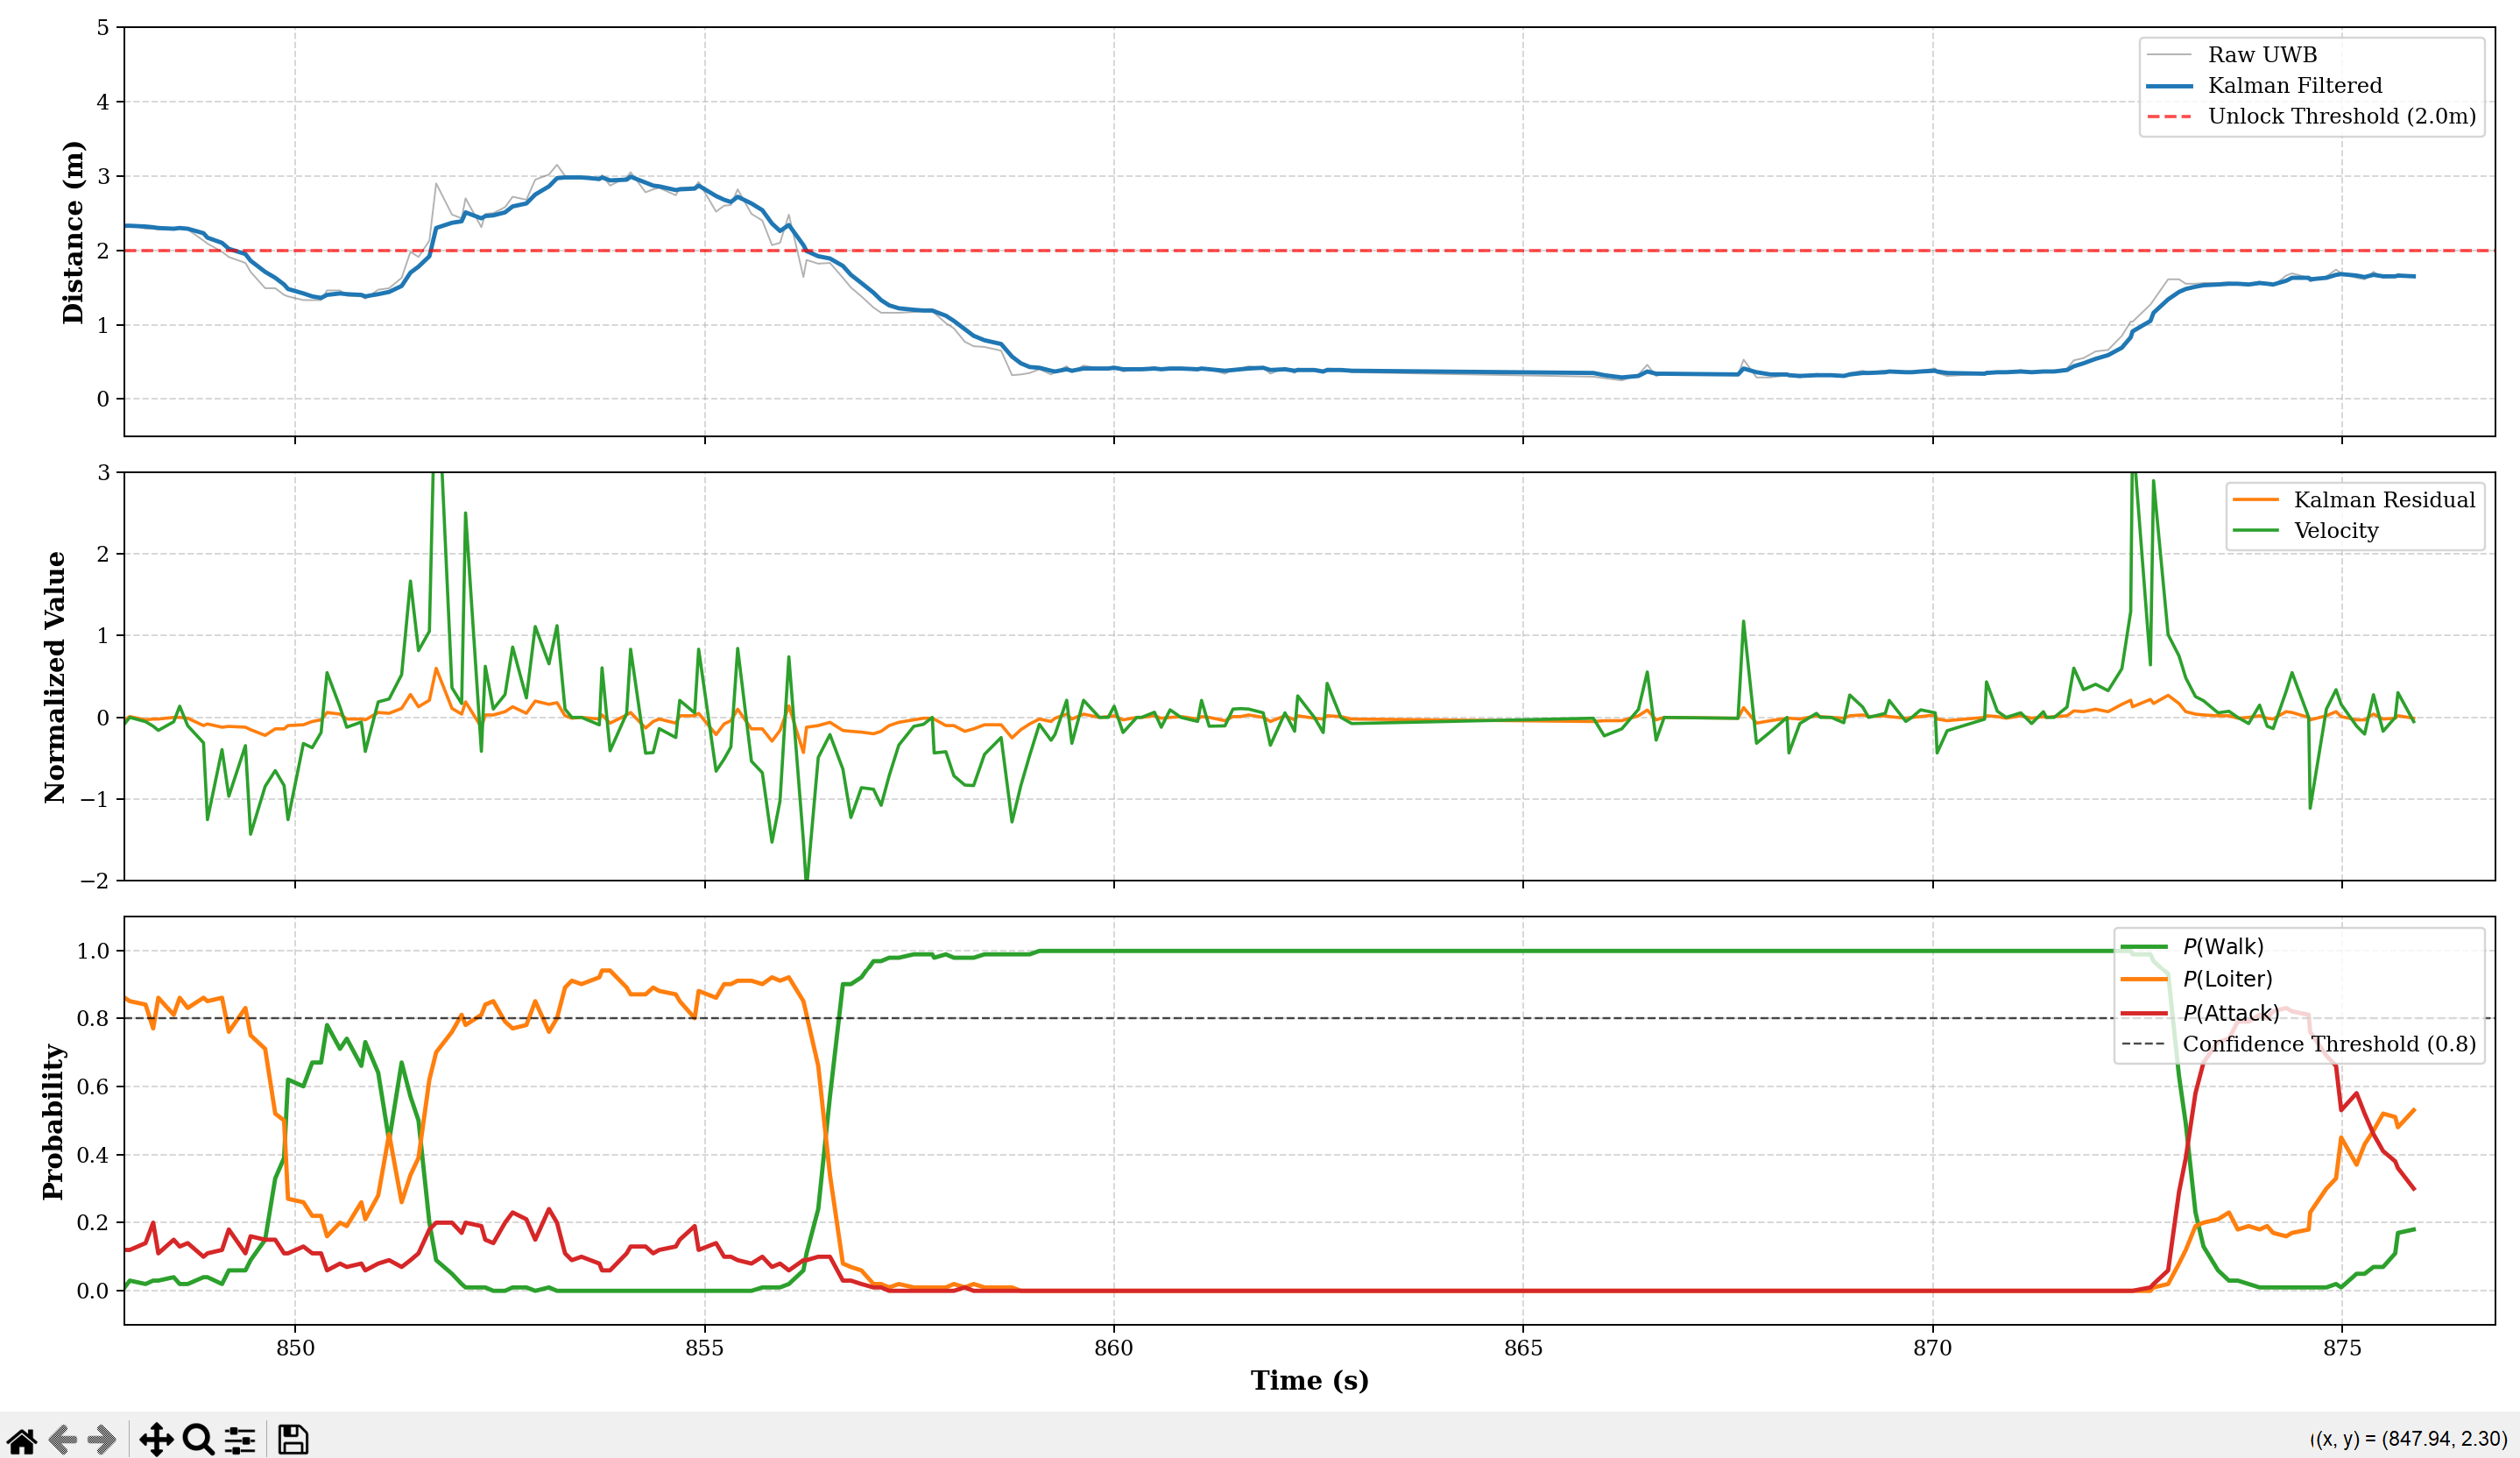
\includegraphics[width=0.8\textwidth]{image/section5/kalman_filter.png}
%     \caption{Đồ thị đối chứng dữ liệu UWB thô và dữ liệu sau bộ lọc Kalman}
%     \label{fig:ai_result}
% \end{figure}

% Sự kết hợp giữa bộ lọc Kalman và tầng nhận diện ý định TinyML (\textbf{đang hiện thực}) hướng tới nâng tầm hệ thống từ một thiết bị đo khoảng cách thuần túy thành một hệ thống nhận thức ngữ cảnh (Context-aware). Các kết quả kiểm thử trên đã chứng minh sự vận hành ổn định và tính đúng đắn của toàn bộ kiến trúc hệ thống Tri-Radio, đáp ứng toàn diện tiêu chuẩn an ninh nghiêm ngặt dành cho giải pháp truy cập phương tiện thông minh.
\newpage
\chapter{\MakeUppercase{KẾT QUẢ THỰC NGHIỆM VÀ ĐÁNH GIÁ}}
\section{Tổng quan}

Hệ thống Smart Car Access được xây dựng trong đề tài đã đạt được các mục tiêu đề ra, không chỉ đáp ứng đầy đủ về mặt chức năng mà còn thể hiện tính khả thi cao trong việc ứng dụng vào các hệ thống xe thông minh hiện đại. Điểm đột phá của hệ thống là việc ứng dụng kiến trúc \textbf{Tri-Radio (Ba sóng vô tuyến)} theo tiêu chuẩn CCC Digital Key Release 3, vượt qua các rào cản bảo mật của mô hình chìa khóa BLE thuần túy trước đây.

Thông qua việc kết hợp chặt chẽ giữa phần cứng nhúng (ESP32-S3, vi mạch NFC PN532, vi mạch UWB DWM3000), hệ điều hành thời gian thực FreeRTOS, và ứng dụng di động phân luồng (Dual-Isolate), hệ thống mang lại một giải pháp truy cập phương tiện thụ động (Passive Keyless Entry - PKE) an toàn tuyệt đối trước các hình thức tấn công tiếp sóng (Relay Attack), đồng thời duy trì độ trễ thấp và trải nghiệm liền mạch cho người dùng.

Nhìn chung, kết quả đạt được chứng minh hệ thống không chỉ phù hợp với mục tiêu nghiên cứu học thuật mà còn có tiềm năng phát triển thành giải pháp thực tế cấp độ công nghiệp (Industrial-grade), làm tiền đề lý tưởng để triển khai các thuật toán học máy (Machine Learning) nhận diện hành vi trong tương lai.

\par\noindent
\textbf{Source code của dự án:} 
\href{https://github.com/T-K-Nguyen/SmartCarAccess}{\textcolor{blue}{\textbf{Kho mã nguồn trên GitHub}}}

\par\noindent
\textbf{Video demo hệ thống:} 
\href{https://drive.google.com/drive/u/0/folders/1UxYpHjgZSg0lMo_vmYPE1nLQXl4Ya1Jx}{\textcolor{red}{\textbf{Demo hệ thống}}}

\section{Kết quả đạt được}

Sau quá trình nghiên cứu và triển khai, hệ thống đã đáp ứng đầy đủ các yêu cầu khắt khe về bảo mật, tính ổn định và tối ưu tài nguyên. Các kết quả cụ thể đạt được được phân tích theo từng hạng mục như sau.

\subsection{Kết quả về phần cứng và hệ thống nhúng}

Hệ thống phần cứng và firmware đóng vai trò là xương sống của toàn bộ đồ án, đảm bảo tính ổn định và khả năng phản hồi thời gian thực:

\begin{itemize}
    \item \textbf{Giao tiếp đa vô tuyến tốc độ cao:} Nhóm đã cấu hình thành công ma trận UART của ESP32-S3 để điều khiển đồng thời module NFC (UART2 - HSU 115200 bps) và module UWB (UART1 - UCI 115200 bps). Thiết kế này loại bỏ hiện tượng nghẽn cổ chai vật lý khi đọc thẻ NFC hoặc nhận luồng dữ liệu Ranging liên tục từ UWB.
    \item \textbf{Đa nhiệm với FreeRTOS:} Để giải quyết bài toán "nghẽn cổ chai" khi thực hiện các phép toán mật mã nặng (ECC Multiplication) đồng thời với việc duy trì sóng vô tuyến, firmware được chia thành các tác vụ (Tasks) độc lập:
    \begin{itemize}
        \item \textit{Core Task (Priority High):} Duy trì quảng bá BLE, xử lý NFC và giao thức UCI của UWB để đảm bảo phản hồi nhanh nhất.
        \item \textit{Crypto Worker Task (Priority Medium):} Chuyên biệt xử lý tính toán ECDH/ECDSA và HKDF. Việc tách biệt này giúp luồng giao tiếp không bị chặn (non-blocking) trong suốt thời gian tính toán khóa.
    \end{itemize}
    \item \textbf{Cơ chế lưu trữ an toàn (Secure Storage):} Tận dụng phân vùng NVS (Non-Volatile Storage) của ESP32 để lưu trữ các thông tin nhạy cảm (Public Key của điện thoại, Fast Path Artifacts, CCC Mailbox). Dữ liệu được bảo vệ bởi cơ chế check-sum, đảm bảo toàn vẹn dữ liệu ngay cả khi mất điện đột ngột.
    \item \textbf{Bộ lọc Hysteresis mở cửa:} Module \texttt{UwbDoorUnlock} đã áp dụng thành công màng lọc độ trễ trạng thái đối với dữ liệu UWB. Rơ-le chỉ mở khi liên tiếp 3 chu kỳ đo UWB đều cho khoảng cách an toàn, triệt tiêu hoàn toàn hiện tượng rơ-le đóng/ngắt liên tục do dao động sóng.
\end{itemize}

\subsection{Kết quả về giao thức bảo mật và mật mã}

Hệ thống đã thiết lập thành công một kiến trúc bảo mật đa lớp, bảo vệ hệ thống xuyên suốt cả 3 giao thức sóng vô tuyến:

\begin{itemize}
    \item \textbf{Thiết lập niềm tin vật lý (Phase A - NFC):} Tuân thủ chuẩn giao tiếp ISO/IEC 14443-4, hệ thống triển khai ngăn xếp APDU với luồng kiểm tra \texttt{SELECT AID} nghiêm ngặt. Xác thực chữ ký số được tối ưu hóa với thư viện mbedTLS, sử dụng thuật toán ECDSA (đường cong secp256r1) và SHA-256 để chống giả mạo khóa.
    \item \textbf{Bảo mật chuyển tiếp hoàn hảo (Phase B - BLE):} Hệ thống không sử dụng khóa tĩnh để mã hóa dữ liệu. Thay vào đó, cơ chế Ephemeral ECDH được áp dụng để sinh cặp khóa dùng một lần. Hàm dẫn xuất khóa HKDF-SHA256 phân tách bí mật chung thành Session Encryption Key (AES-GCM) và Session MAC Key (HMAC), đảm bảo tính bí mật chuyển tiếp (Forward Secrecy) và chống tấn công phát lại (Anti-Replay).
    \item \textbf{Chống tấn công tiếp sóng (Phase C \& D - UWB):} Thời gian bay (ToF) của sóng UWB là bất biến. Nhờ giao thức DS-TWR và việc ứng dụng chuỗi STS (Scrambled Timestamp Sequence) được dẫn xuất từ khóa của Phase B, mọi nỗ lực của kẻ gian nhằm dùng trạm lặp (Relay Station) để khuếch đại sóng và đánh lừa khoảng cách đều bị vô hiệu hóa ở lớp vật lý.
\end{itemize}

\subsection{Kết quả về Ứng dụng di động và tích hợp hệ thống}
\subsubsection{Ứng dụng di động}
Ứng dụng di động được phát triển bằng Flutter với định hướng tối ưu trải nghiệm người dùng (User Experience) và khả năng tương tác trực quan với hệ thống Smart Car Access. Giao diện được thiết kế theo phong cách hiện đại, tối giản và tập trung vào các thao tác truy cập nhanh, phù hợp với đặc thù của một hệ thống truy cập phương tiện thông minh.

Bên cạnh việc hỗ trợ các chức năng cốt lõi như quản lý khóa số (Digital Key), xác thực thiết bị và theo dõi trạng thái xe theo thời gian thực, ứng dụng còn cung cấp khả năng tùy chỉnh giao diện và cấu hình cá nhân nhằm nâng cao tính tiện dụng trong quá trình sử dụng hằng ngày.

\begin{figure}[H]
    \centering
    
    % ================= ROW 1 =================
    \begin{minipage}[t]{0.25\textwidth}
        \centering
        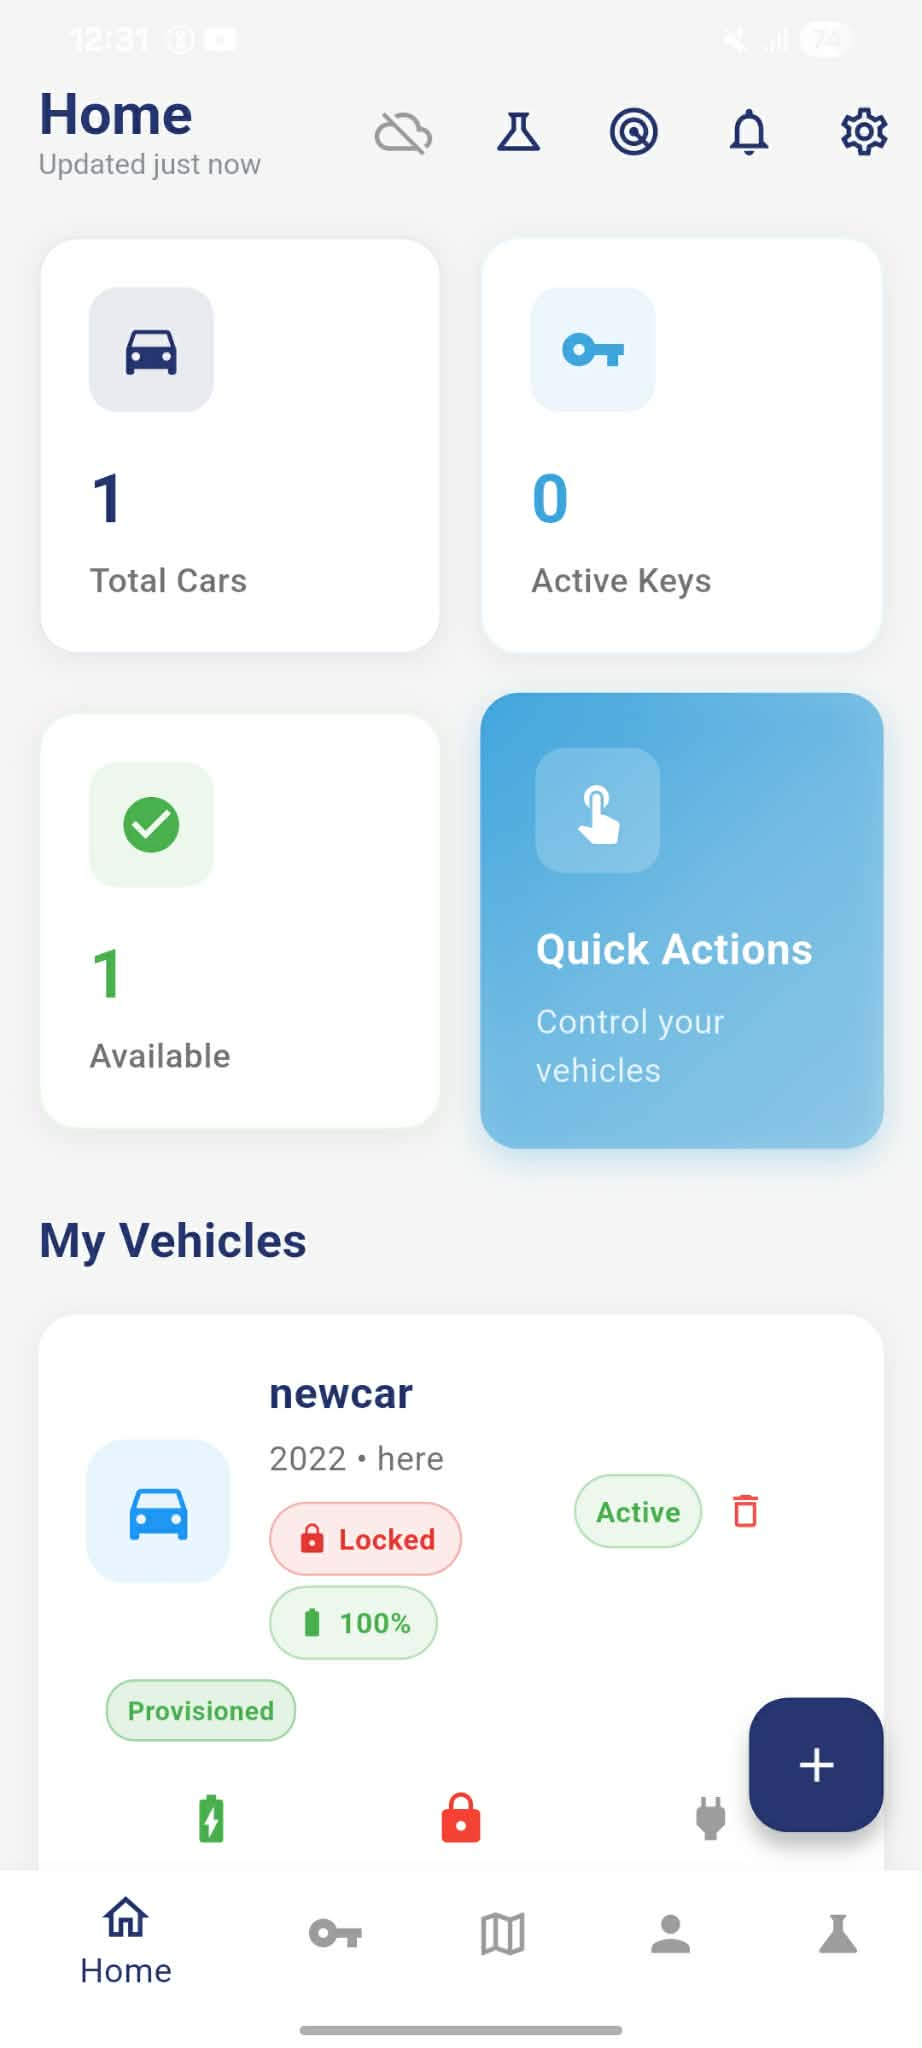
\includegraphics[width=\linewidth]{image/section5/home.jpg}
        \caption{Giao diện màn hình chính}
        \label{fig:app_home}
    \end{minipage}
    \hfill
    \begin{minipage}[t]{0.25\textwidth}
        \centering
        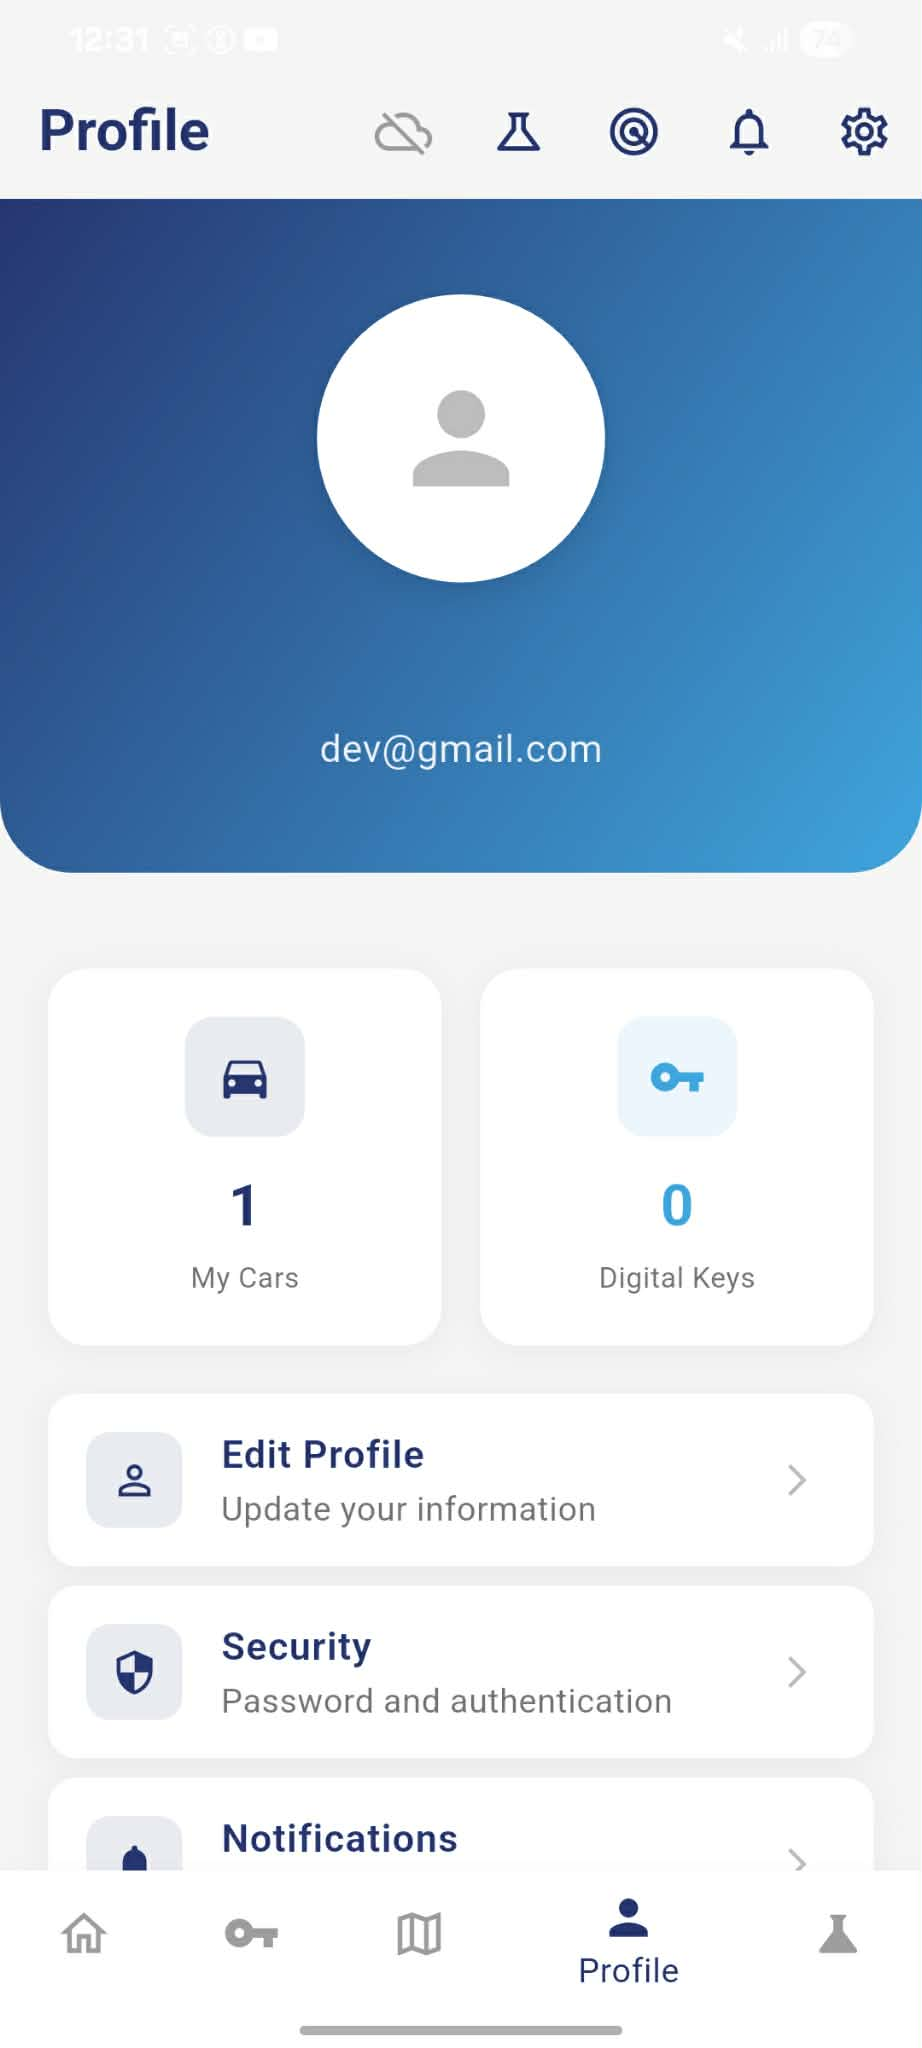
\includegraphics[width=\linewidth]{image/section5/profile2.jpg}
        \caption{Giao diện hồ sơ người dùng (1)}
        \label{fig:app_profile2}
    \end{minipage}
    \hfill
    \begin{minipage}[t]{0.25\textwidth}
        \centering
        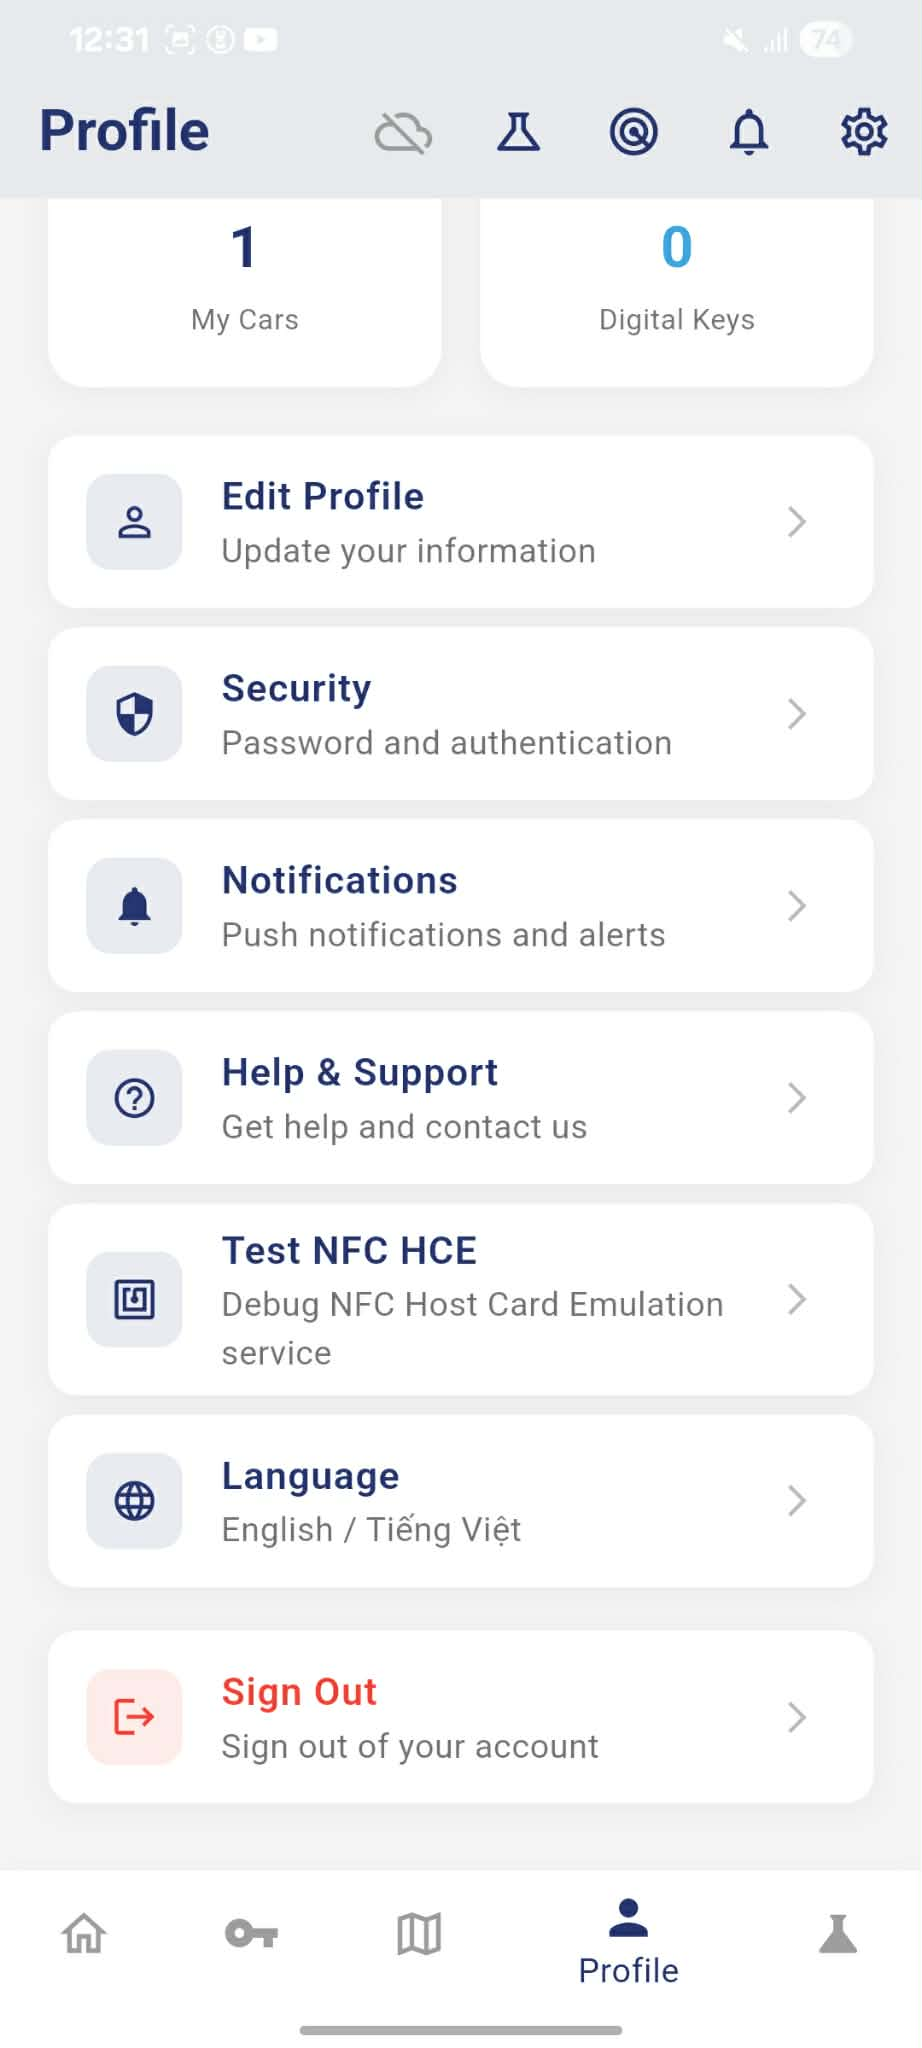
\includegraphics[width=\linewidth]{image/section5/profile.jpg}
        \caption{Giao diện hồ sơ người dùng (2)}
        \label{fig:app_profile}
    \end{minipage}

\end{figure}

\begin{figure}[H]
    \centering

    % ================= ROW 2 =================
    \begin{minipage}[t]{0.25\textwidth}
        \centering
        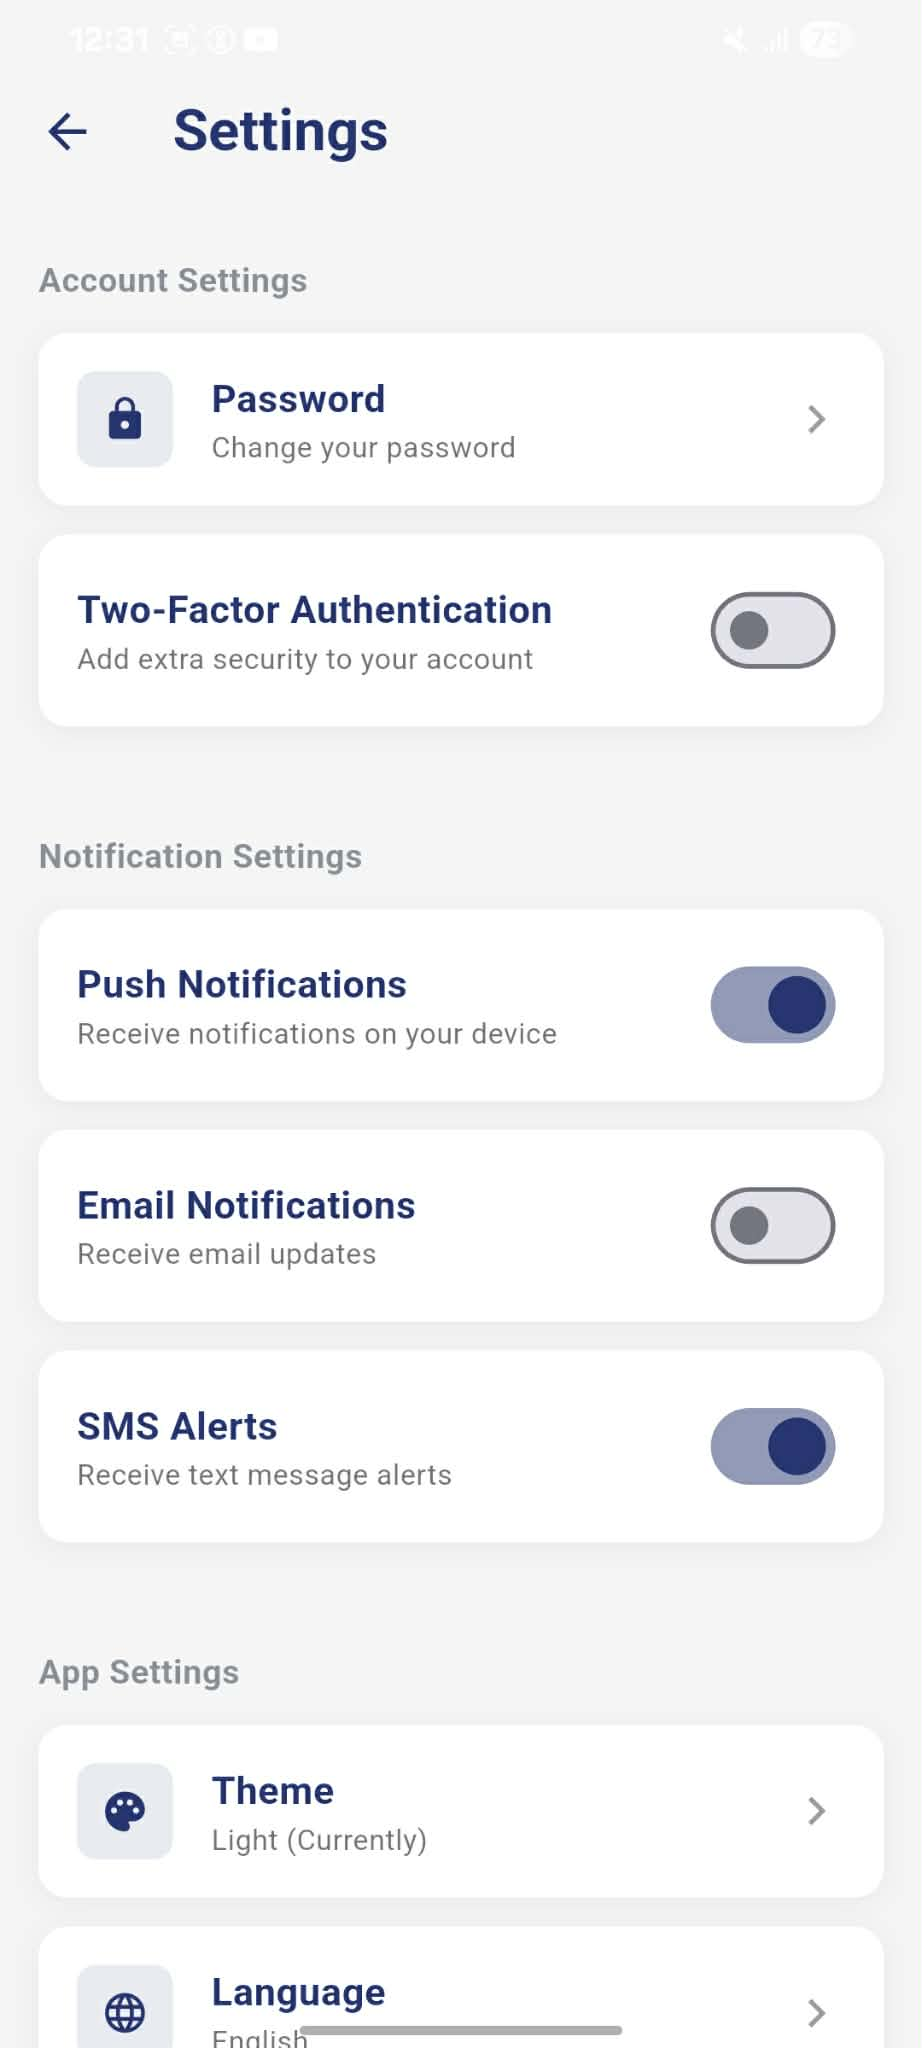
\includegraphics[width=\linewidth]{image/section5/setting.jpg}
        \caption{Giao diện cài đặt hệ thống (1)}
        \label{fig:app_setting1}
    \end{minipage}
    \hfill
    \begin{minipage}[t]{0.25\textwidth}
        \centering
        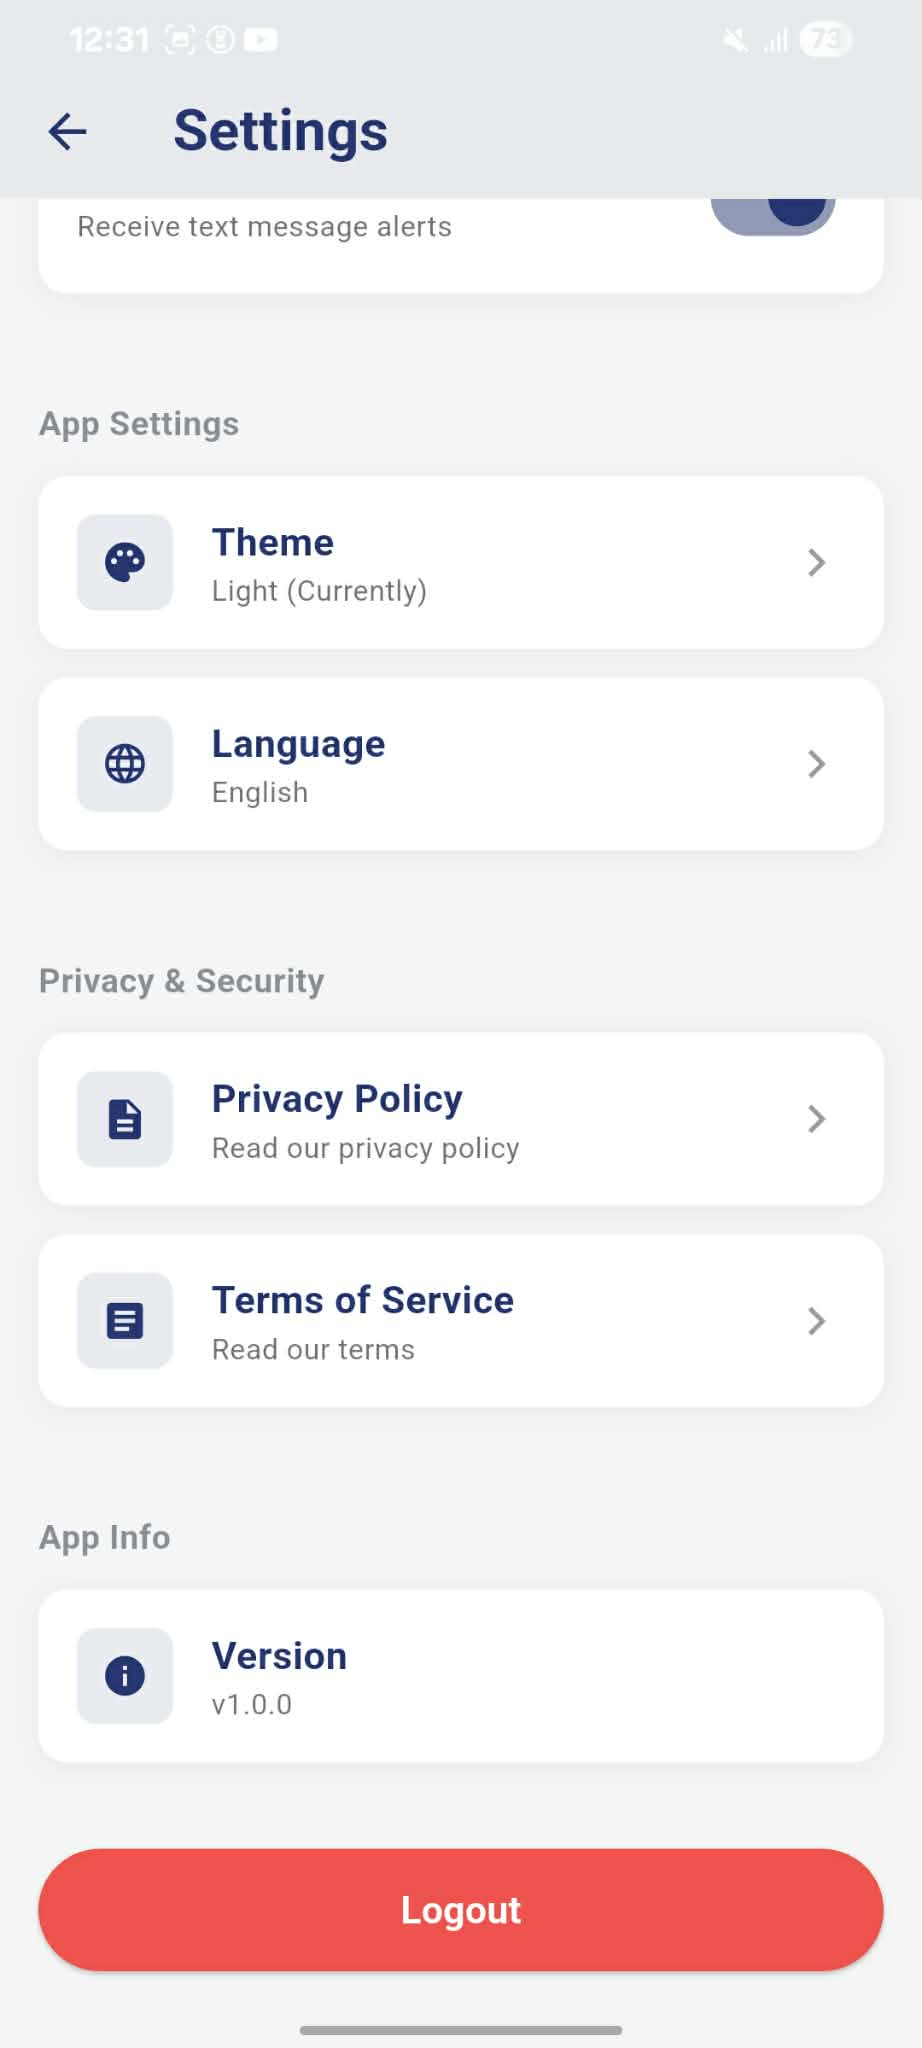
\includegraphics[width=\linewidth]{image/section5/setting2.jpg}
        \caption{Giao diện cài đặt hệ thống (2)}
        \label{fig:app_setting2}
    \end{minipage}
    \hfill
    \begin{minipage}[t]{0.25\textwidth}
        \centering
        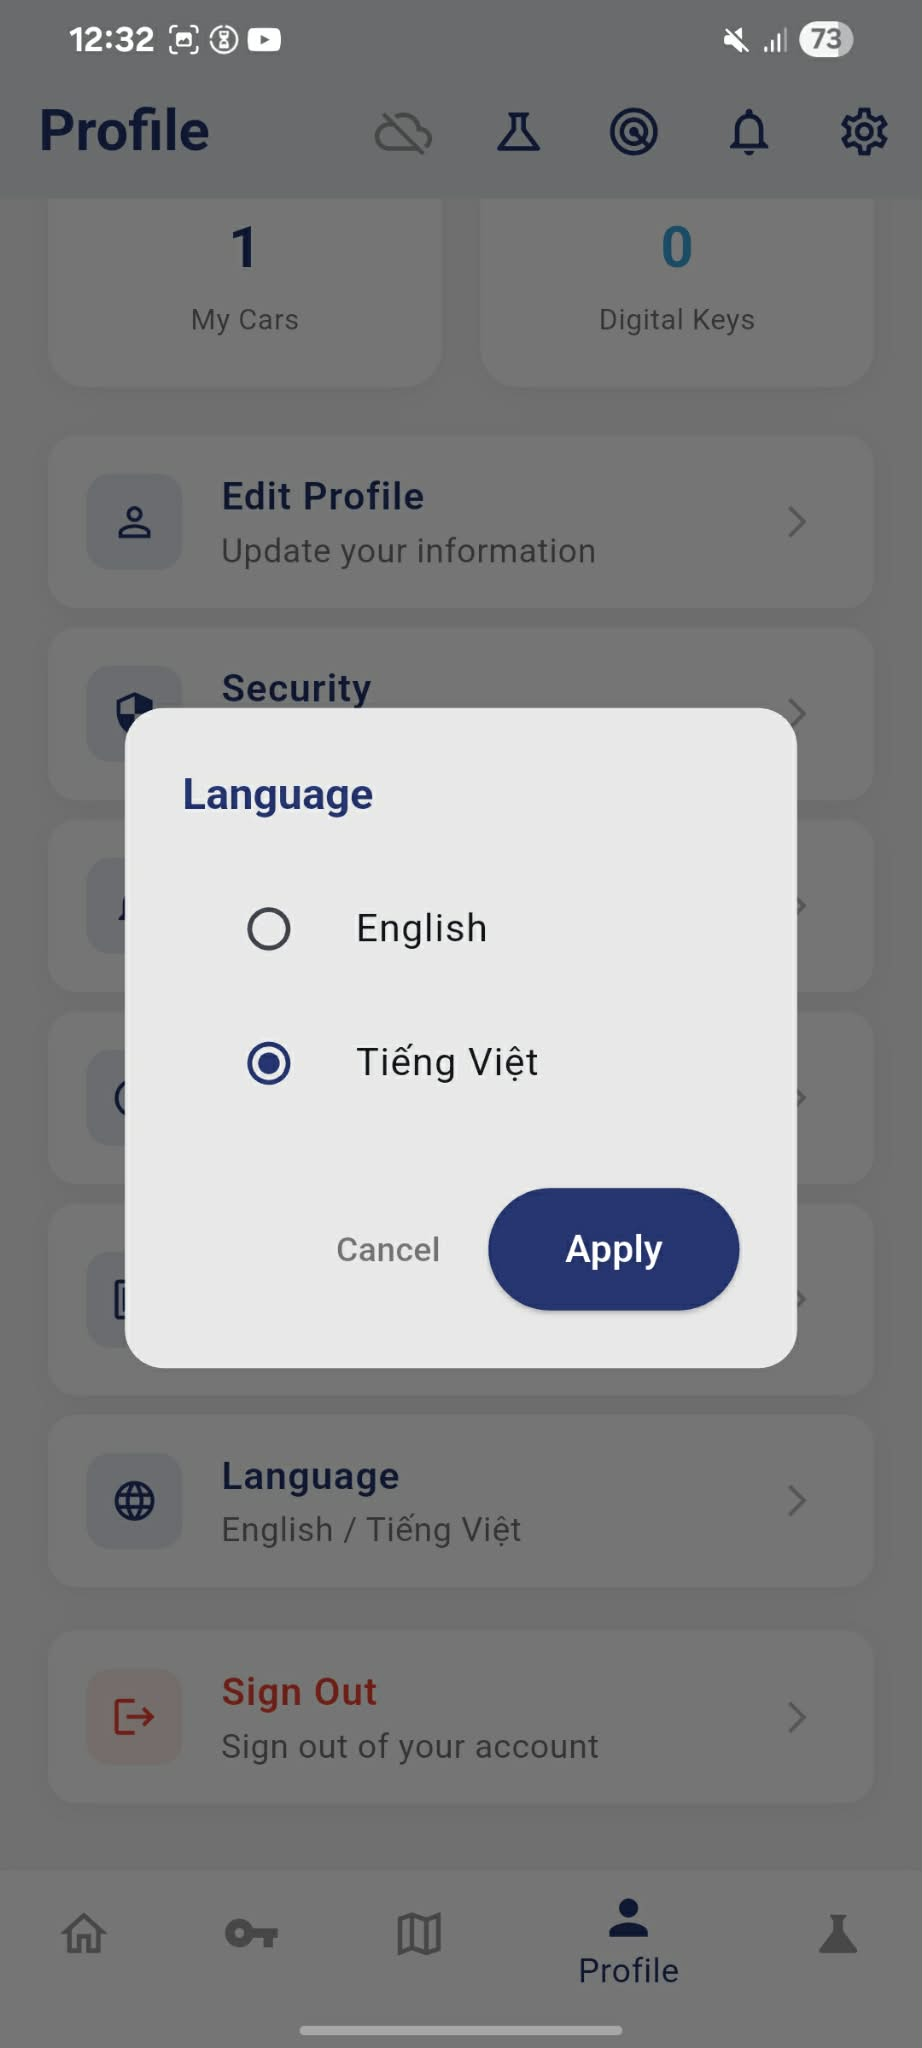
\includegraphics[width=\linewidth]{image/section5/language.jpg}
        \caption{Giao diện lựa chọn ngôn ngữ}
        \label{fig:app_language}
    \end{minipage}

\end{figure}
\subsubsection{Tích hợp hệ thống}

Ứng dụng di động (Flutter) không chỉ cung cấp giao diện tương tác mà còn đóng vai trò là thiết bị đầu cuối thông minh (Intelligent Terminal):

\begin{itemize}
    \item \textbf{Kiến trúc hướng sự kiện và Đồng bộ thời gian thực:} Dựa trên luồng dữ liệu (Streams) của Flutter và kiến trúc Serverless (Firebase), cơ chế Snapshot Listener của Cloud Firestore đồng bộ trạng thái xe và quyền truy cập (Digital Key) gần như tức thời (Near real-time) mà không gây chặn luồng giao diện (UI Thread blocking).
    
    \item \textbf{Hiện thực hóa HCE tại tầng Hệ điều hành:} Thay vì phụ thuộc vào Secure Element (SE) của phần cứng, nhóm đã xây dựng thành công dịch vụ nền Host Card Emulation (HCE) trên Android. Dịch vụ HCE được đăng ký với Hệ điều hành thông qua AID cụ thể, đảm bảo hệ thống chỉ phản hồi các yêu cầu từ xe của chủ sở hữu.
    
    \item \textbf{Tích hợp Android Keystore System (TEE):} Khóa Private Key không lưu trữ trong mã nguồn ứng dụng mà được sinh ra và bảo vệ trong Trusted Execution Environment của điện thoại. Khi cần ký số ECDSA, Flutter gửi yêu cầu xuống tầng Native qua MethodChannel, đảm bảo vật liệu khóa không bao giờ bị trích xuất ngay cả khi thiết bị bị root.
    
    \item \textbf{Kiến trúc Dual-Isolate (Handoff PKE):} Việc tách tiến trình quét BLE xuống Background Service cho phép trải nghiệm "Mở khóa thụ động" thực sự. Khi Background xác thực BLE xong, luồng Foreground được đánh thức để lập tức tiếp quản kết nối và cấu hình chip UWB (OOB Payload) mà không cần quét lại thiết bị, giảm độ trễ chuyển giao xuống dưới 400ms.
\end{itemize}

\subsection{Đánh giá hiệu năng và Tính ổn định}

Nhóm thực hiện đã tiến hành đo đạc thực nghiệm trong môi trường phòng thí nghiệm với thiết bị ESP32-S3 (240MHz) và Smartphone Android.

\subsubsection{Phân tích tốc độ giao dịch và độ trễ toàn trình}
Dựa trên tiêu chuẩn CCC, hệ thống được thiết kế để hỗ trợ cả hai luồng xác thực. Kết quả thực nghiệm qua log phân tích cho thấy độ trễ được tối ưu hóa cực kỳ tốt:

\begin{itemize}
    \item \textbf{Tốc độ Giao dịch tiêu chuẩn (Standard Transaction):} Đây là luồng xác thực đầy đủ (Full Handshake) khi hai thiết bị kết nối lần đầu. ESP32 thực hiện toàn bộ quá trình trao đổi khóa Ephemeral, tính toán ECDH, chạy HKDF và xác minh chữ ký phần cứng ECDSA từ điện thoại. Kết quả đo đạc cho thấy tổng thời gian từ lúc nhận gói \texttt{AUTH0} đến khi chốt sổ \texttt{CONTROL\_FLOW\_ack} chỉ mất $\approx 1.56$ giây. Thời gian xử lý mật mã thuần túy trên ESP32 chỉ chiếm $\approx 480$ ms, phần còn lại là độ trễ truyền tải BLE.
    \leavevmode
    \begin{table}[!htbp]
        \centering
        \caption{Thời gian xử lý thực tế quá trình Mở khóa thụ động (Giao dịch Tiêu chuẩn)}
        \label{tab:latency_breakdown_real}
        \begin{tabular}{|l|p{6.5cm}|c|}
            \hline
            \textbf{Giai đoạn} & \textbf{Mô tả tác vụ} & \textbf{Thời gian trung bình} \\
            \hline
            1. BLE Connection & Điện thoại vào vùng phủ sóng ($\approx 10$m) và kết nối GATT. & $\approx 800 - 1200$ ms \\
            \hline
            2. Crypto Handshake & Tính toán ECDH, HKDF và trao đổi chữ ký (Phase B). & $\approx 480$ ms (Chỉ phần xử lý) \\
            \hline
            3. UWB Handoff & Gửi OOB Payload qua BLE và cấu hình chip DWM3000. & $\approx 200 - 300$ ms \\
            \hline
            4. Secure Ranging & Đo UWB liên tục (Tần số $10\sim15$ Hz) đến khi khoảng cách $\le 2.0$m. & Tùy tốc độ di chuyển \\
            \hline
            5. Access Decision & Lọc Hysteresis (đợi 3 chu kỳ đo liên tiếp) và bật GPIO Relay. & $\approx 200 - 300$ ms \\
            \hline
        \end{tabular}
    \end{table}
    \item \textbf{Tốc độ Giao dịch nhanh (Fast Transaction):} Đối với các lần kết nối lại (Reconnect), hệ thống tận dụng \textit{Fast Path Artifact} đã thiết lập từ trước, bỏ qua các phép toán bất đối xứng (Asymmetric Crypto) nặng nề để chuyển sang xác thực đối xứng (Symmetric Crypto). Điều này giúp rút ngắn thời gian xác thực kênh truyền BLE (Phase B) xuống mức $\approx 800 - 900$ ms, tăng tốc đáng kể quá trình bàn giao (Handoff) sang UWB.
\end{itemize}



\noindent \textbf{Nhận xét:} Ngay khi người dùng bước vào vùng Welcome Zone (10m), hệ thống chỉ mất chưa tới 2 giây để hoàn tất xác thực mật mã ngầm. Khi tiếp cận sát xe, hệ thống phản hồi mở cửa qua UWB gần như tức thời (khoảng 300ms) khi người dùng đi bước vào vùng 2m.

\vspace{0.5cm}
\noindent \textbf{Đánh giá chuyên sâu về Độ trễ chuyển giao (Handoff Latency Breakdown):}

Bên cạnh thời gian giao dịch tổng thể, một chỉ số đặc biệt quan trọng trong tiêu chuẩn CCC là thời gian bàn giao (Handoff) từ kênh kết nối BLE sang kênh đo đạc UWB. Nhóm đã thực hiện trích xuất log thực tế (System Telemetry) để phân rã các điểm nghẽn (Bottleneck) trong quá trình này.



\leavevmode
\begin{table}[!htbp]
    \centering
    \caption{Phân rã độ trễ chuyển giao từ BLE sang UWB (Dựa trên Log thực nghiệm)}
    \label{tab:handoff_latency_breakdown}
    \begin{tabularx}{\textwidth}{|c|L|c|L|}
        \hline
        \textbf{Giai đoạn} & \textbf{Sự kiện / Tác vụ} & \textbf{Độ trễ} & \textbf{Phân tích \& Nguyên nhân} \\
        \hline
        1 & Nhận cấu hình OOB \& Chờ Hệ điều hành của điện thoại & $\approx 584$ ms & Thời gian chờ hệ điều hành (Android) khởi động chip UWB, cấp phát tài nguyên dịch vụ FiRa/CCC và chuẩn bị ăng-ten. \\
        \hline
        2 & ESP32 thực thi cấu hình UCI (Firmware Execution) & $\approx 30$ ms & ESP32 thiết lập FSM và truyền toàn bộ chuỗi lệnh cấu hình UCI (Session, App, Ranging) xuống DWM3000 qua UART. \\
        \hline
        3 & Bắt khung hình UWB đầu tiên (Time-to-First-Fix) & $\approx 16$ ms & DWM3000 hoàn tất khởi động, bắt sóng từ điện thoại và trả về khung dữ liệu đo khoảng cách (Ranging) đầu tiên. \\
        \hline
        \multicolumn{2}{|r|}{\textbf{Tổng độ trễ chuyển giao:}} & \textbf{$\approx 630$ ms} & \textbf{Đạt chuẩn CCC ($< 1.5$s)} \\
        \hline
    \end{tabularx}
\end{table}

\noindent \textbf{Nhận xét:} 
Dữ liệu thực nghiệm từ Bảng \ref{tab:handoff_latency_breakdown} cho thấy kiến trúc phân luồng hoạt động với hiệu suất tối ưu. Phần lớn thời gian chờ của quá trình Handoff ($\approx 584$ ms) là độ trễ khách quan thuộc về kiến trúc cấp phát tài nguyên của hệ điều hành trên thiết bị di động. Ngay khi nhận được lệnh kích hoạt, hệ thống nhúng (ESP32-S3) đáp ứng gần như tức thời với tổng thời gian cấu hình và đo đạc chỉ mất $46$ ms ($30$ ms + $16$ ms). Điều này chứng minh Firmware và các tác vụ FreeRTOS được thiết kế rất chặt chẽ, khai thác tối đa băng thông phần cứng mà không xảy ra hiện tượng kẹt luồng (blocking) hay suy hao hiệu năng.

\subsubsection{Đánh giá tài nguyên hệ thống (Resource Utilization):}
Việc tối ưu hóa bộ nhớ là rất quan trọng đối với các hệ thống nhúng Automotive.

\leavevmode
\begin{table}[H]
    \centering
    \caption{Thống kê tiêu thụ tài nguyên trên ESP32-S3}
    \label{tab:resource_usage}
    \begin{tabular}{|l|c|c|c|}
        \hline
        \textbf{Loại tài nguyên} & \textbf{Tổng dung lượng} & \textbf{Đã sử dụng} & \textbf{Tỷ lệ (\%)} \\
        \hline
        Flash (Program) & 8 MB & $\approx 1.2$ MB & $\approx 15\%$ \\
        \hline
        Static RAM & 512 KB & $\approx 95$ KB & $\approx 18.5\%$ \\
        \hline
        Stack (Crypto Task) & 12 KB (Allocated) & $\approx 8.5$ KB (Peak) & $70.8\%$ \\
        \hline
    \end{tabular}
\end{table}
\textit{Đánh giá:} Hệ thống vẫn còn dư lượng lớn tài nguyên Flash và RAM, tạo tiền đề sẵn sàng tích hợp các mô hình Machine Learning mạnh hơn trực tiếp lên vi điều khiển ở các nghiên cứu tiếp theo.


\subsubsection{Đánh giá tiêu thụ năng lượng (Power Consumption)}

Trong môi trường ứng dụng ô tô, việc kiểm soát dòng tiêu thụ là tiêu chí tiên quyết để đảm bảo không gây cạn kiệt nguồn ắc-quy (lead-acid battery) khi xe dừng đỗ lâu ngày. Hệ thống được thiết kế tối ưu hóa dựa trên các chế độ vận hành của vi điều khiển ESP32-S3 và quản lý trạng thái của các module NFC, BLE, UWB.

\begin{itemize}
    \item \textbf{Chế độ Deep Sleep (Chế độ chờ dài hạn):} Đây là trạng thái tiêu thụ năng lượng thấp nhất. Hệ thống tắt toàn bộ các radio (NFC, BLE, UWB) và đưa CPU về trạng thái ngủ sâu, chỉ duy trì bộ đếm thời gian thực (RTC) hoặc chờ kích hoạt từ ngoại vi (NFC field hoặc nút nhấn tay nắm cửa). Dòng điện tiêu thụ ở mức cực thấp ($< 0.1$ mA), cho phép xe duy trì trạng thái này trong nhiều tháng mà không ảnh hưởng đến dung lượng ắc-quy.
    
    \item \textbf{Chế độ Idle - BLE Advertising (Chế độ chờ tiệm cận):} Khi hệ thống phát hiện có sự tương tác gần hoặc theo lịch trình, BLE sẽ bắt đầu quảng bá (Advertising) để điện thoại có thể nhận diện. Dòng tiêu thụ trung bình lúc này khoảng $75$ mA do phải duy trì chu kỳ quét và phát sóng RF định kỳ. Nhóm đã tối ưu hóa bằng cách tăng chu kỳ quảng bá (Advertising Interval) để cân bằng giữa tốc độ kết nối và năng lượng tiêu thụ.
    
    \item \textbf{Chế độ Active - Secure Ranging (Chế độ hoạt động toàn phần):} Đây là giai đoạn tiêu tốn năng lượng nhất khi hệ thống đồng thời thực hiện xác thực mật mã ECDH/ECDSA trên CPU (chạy ở xung nhịp 240MHz) và kích hoạt vi mạch DWM3000 để đo khoảng cách liên tục. Dòng điện đạt đỉnh $\approx 140$ mA. Tuy nhiên, nhờ kiến trúc phân tầng (Phase C/D), giai đoạn này chỉ diễn ra trong thời gian ngắn (vài giây) khi người dùng tiếp cận sát xe, nên tổng năng lượng tiêu thụ tích phân theo thời gian vẫn nằm trong ngưỡng an toàn.
\end{itemize}

\leavevmode
\begin{table}[H]
    \centering
    \caption{Phân tích dòng tiêu thụ chi tiết ở các chế độ (Nguồn cấp 5V qua LDO)}
    \label{tab:power_consumption}
    \begin{tabular}{|l|p{6cm}|c|}
        \hline
        \textbf{Chế độ hoạt động} & \textbf{Chi tiết trạng thái phần cứng} & \textbf{Dòng điện (mA)} \\
        \hline
        Deep Sleep & Tắt RF, CPU Off, chỉ duy trì RTC/ULP. & $< 0.1$ mA \\
        \hline
        Idle (Advertising) & BLE Advertising (Interval 100ms), CPU 80MHz. & $\approx 75$ mA \\
        \hline
        Active (Crypto) & Thực hiện xác thực ECDSA, CPU 240MHz. & $\approx 110$ mA \\
        \hline
        Active (Ranging) & Đo UWB liên tục + Suy luận TinyML. & $\approx 140$ mA \\
        \hline
    \end{tabular}
\end{table}

\textit{Nhận xét:} Với dòng tiêu thụ tĩnh ở chế độ Deep Sleep cực thấp, hệ thống hoàn toàn đáp ứng được các tiêu chuẩn khắt khe về quản lý năng lượng trên xe hơi hiện đại, đảm bảo tính bền bỉ và ổn định của nguồn điện hệ thống.


\subsubsection{Độ ổn định, Phạm vi kết nối và Tối ưu dữ liệu UWB}
\begin{itemize}
    \item \textbf{Xác định sai số hệ thống (Systematic Offset):} Để đảm bảo tính chính xác tuyệt đối cho dữ liệu đầu vào, nhóm đã thực hiện quy trình hiệu chuẩn thực nghiệm. Phương pháp thực hiện bao gồm việc đo đạc tại các mốc khoảng cách chuẩn $1m, 2m$ và $3m$. Tại mỗi mốc, dữ liệu được lấy trung bình từ 3 lần đo độc lập nhằm triệt tiêu các sai số ngẫu nhiên. Kết quả phân tích cho thấy hệ thống tồn tại một sai số cố định (offset) là $24$ cm. Giá trị này đã được tích hợp vào firmware để bù trừ trực tiếp vào dữ liệu thô trước khi đưa vào các tầng lọc phía sau.
    
    \item \textbf{Phạm vi kết nối BLE:} Kết nối ổn định ở khoảng cách $40 \sim 50$ mét (môi trường thoáng) và $10 \sim 15$ mét (xuyên qua kính/thân xe).
    
    \item \textbf{Độ tin cậy hệ thống:} Thực hiện 10 lần đóng/mở khóa liên tục, kết hợp giả lập ngắt kết nối đột ngột. Hệ thống tự phục hồi trạng thái FSM 10/10 lần, không xảy ra hiện tượng treo (hang).
    
    \item \textbf{Độ ổn định của dữ liệu Ranging sau khi áp dụng Kalman Filter:} Dữ liệu khoảng cách gốc từ vi mạch DWM3000 thường tồn tại các dao động nhiễu tĩnh ($\pm 10\sim20$ cm) hoặc các bước nhảy vọt do hiện tượng phản xạ đa đường (multipath). Nhóm đã tích hợp thành công \textbf{Bộ lọc Kalman 1D} trực tiếp vào tầng Parse gói tin UCI (với ma trận hiệp phương sai được tinh chỉnh riêng cho bước đi của người: Process Noise $Q=0.05$, Sensor Noise $R=0.2$). Kết quả cho thấy đường cong quỹ đạo (trajectory) của người dùng trở nên cực kỳ mượt mà. Kỹ thuật này không chỉ giúp bộ đệm Hysteresis ra quyết định mở cửa chính xác tuyệt đối mà còn tạo ra giá trị thặng dư (Residual) chất lượng cao, phục vụ làm đầu vào (Input feature) cho mạng nơ-ron LSTM nhận diện hành vi giả mạo trong tương lai.
\end{itemize}



%-------------------------------------------------------------------------------------------------------------



\subsection{Ứng dụng TinyML trong nhận diện hành vi và phòng chống tấn công tiếp sóng chuyên sâu}

Điểm nhấn kỹ thuật quan trọng nhất của đồ án là việc triển khai thành công mô hình học máy nhúng (TinyML) trực tiếp trên vi điều khiển ESP32-S3. Thay vì chỉ dựa vào các ngưỡng khoảng cách cố định (Rule-based), hệ thống hiện nay có khả năng "hiểu" được hình thái động học của người dùng thông qua chuỗi thời gian.

\begin{itemize}
    \item \textbf{Xây dựng bộ dữ liệu đặc trưng (Dataset \& Feature Engineering):} Nhóm đã thực hiện thu thập và gán nhãn cho hơn $4.000$ chuỗi dữ liệu thực tế (sequences), bao gồm 3 trạng thái chính: \textit{Tiếp cận xe (Walk)}, \textit{Lảng vảng không mục đích (Loiter)} và \textit{Tấn công tiếp sóng (Relay Attack)}. Các đặc trưng đầu vào được tối ưu hóa bao gồm: Khoảng cách đã lọc Kalman, Thặng dư (Residual) từ bộ lọc, và Vận tốc tức thời (Velocity).
    
    \item \textbf{Kiến trúc mô hình tối ưu cho phần cứng nhúng:} Nhóm đã hiện thực hóa mạng nơ-ron tích chập một chiều (1D-CNN) thông qua thư viện TensorFlow Lite for Microcontrollers (TFLM). Với cửa sổ thời gian $25$ khung hình (tương đương $2.5$ giây dữ liệu), mô hình có khả năng trích xuất các đặc trưng không gian-thời gian để phân biệt các hành vi có quỹ đạo tương đồng nhưng bản chất vật lý khác nhau.
    
    \item \textbf{Kết quả thực nghiệm suy luận tại biên (On-device Inference):}
    \begin{itemize}
        \item \textit{Độ chính xác:} Mô hình đạt độ chính xác tổng thể là \textbf{84.3\%} trên tập dữ liệu kiểm thử độc lập. Đặc biệt, chỉ số \textbf{Precision} cho nhãn \textit{Relay Attack} đạt \textbf{96\%}, đảm bảo khả năng phát hiện sớm các hành vi giả mạo tín hiệu có độ trễ vật lý cao.
        
        \item \textit{Hiệu năng phần cứng:} Nhờ kỹ thuật lượng tử hóa và tối ưu vùng nhớ (Tensor Arena), mô hình chỉ chiếm khoảng \textbf{21.5 KB} bộ nhớ Flash và vận hành ổn định trong vùng nhớ tĩnh \textbf{40 KB RAM}. Thời gian suy luận cho mỗi cửa sổ dữ liệu đạt mức mili-giây, hoàn toàn không gây ảnh hưởng đến tính thời gian thực của các tác vụ FreeRTOS.
    \end{itemize}


\begin{figure}[H]
    \centering
    \begin{minipage}{0.45\textwidth}
        \centering
        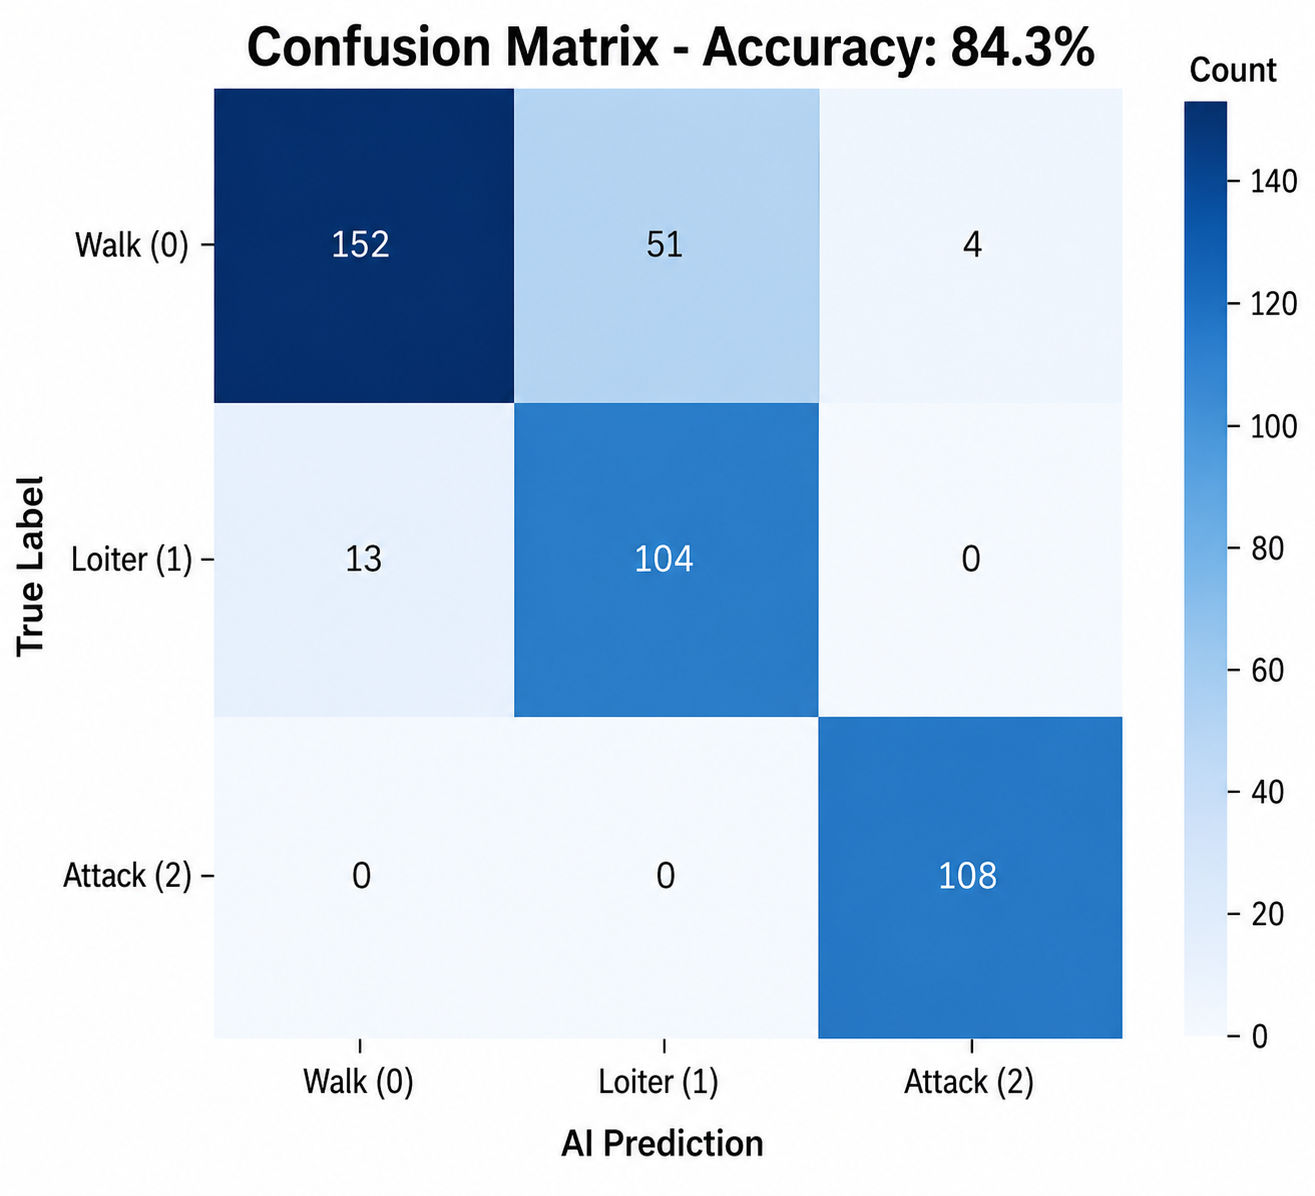
\includegraphics[width=\textwidth]{image/LSTM/training out come.png}
        \caption{Ma trận nhầm lẫn với độ chính xác là 84.3\%}
        \label{fig:confu_matrix}
    \end{minipage}
    \hfill
    \begin{minipage}{0.45\textwidth}
        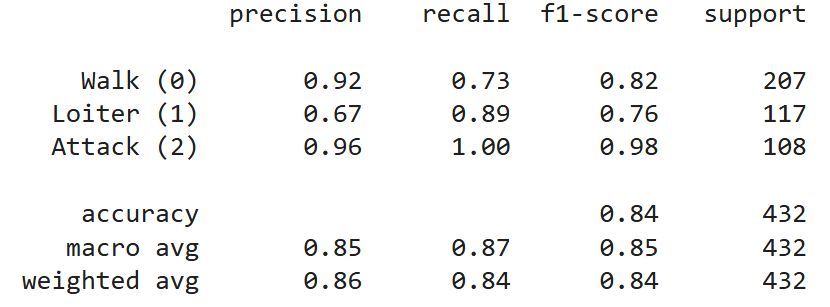
\includegraphics[width=\linewidth]{image/LSTM/baocaophanloai.png}
        \caption{Báo cáo phân loại (walk, loiter, relay attack)}
        \label{fig:classification_report}
    \end{minipage}
\end{figure}
    
    \item \textbf{Phân tích diễn biến suy luận theo thời gian (Time-series Inference Analysis):}
    Để làm rõ cơ chế ra quyết định của hệ thống, nhóm đã trích xuất và trực quan hóa luồng dữ liệu thực tế thông qua các đồ thị đồng bộ hóa trục thời gian. Việc phân tích này giúp minh chứng sự phối hợp chặt chẽ giữa tầng xử lý tín hiệu (Kalman Filter) và tầng nhận diện hành vi (1D-CNN) trong các kịch bản khác nhau.


    \begin{figure}[H]
        \centering
        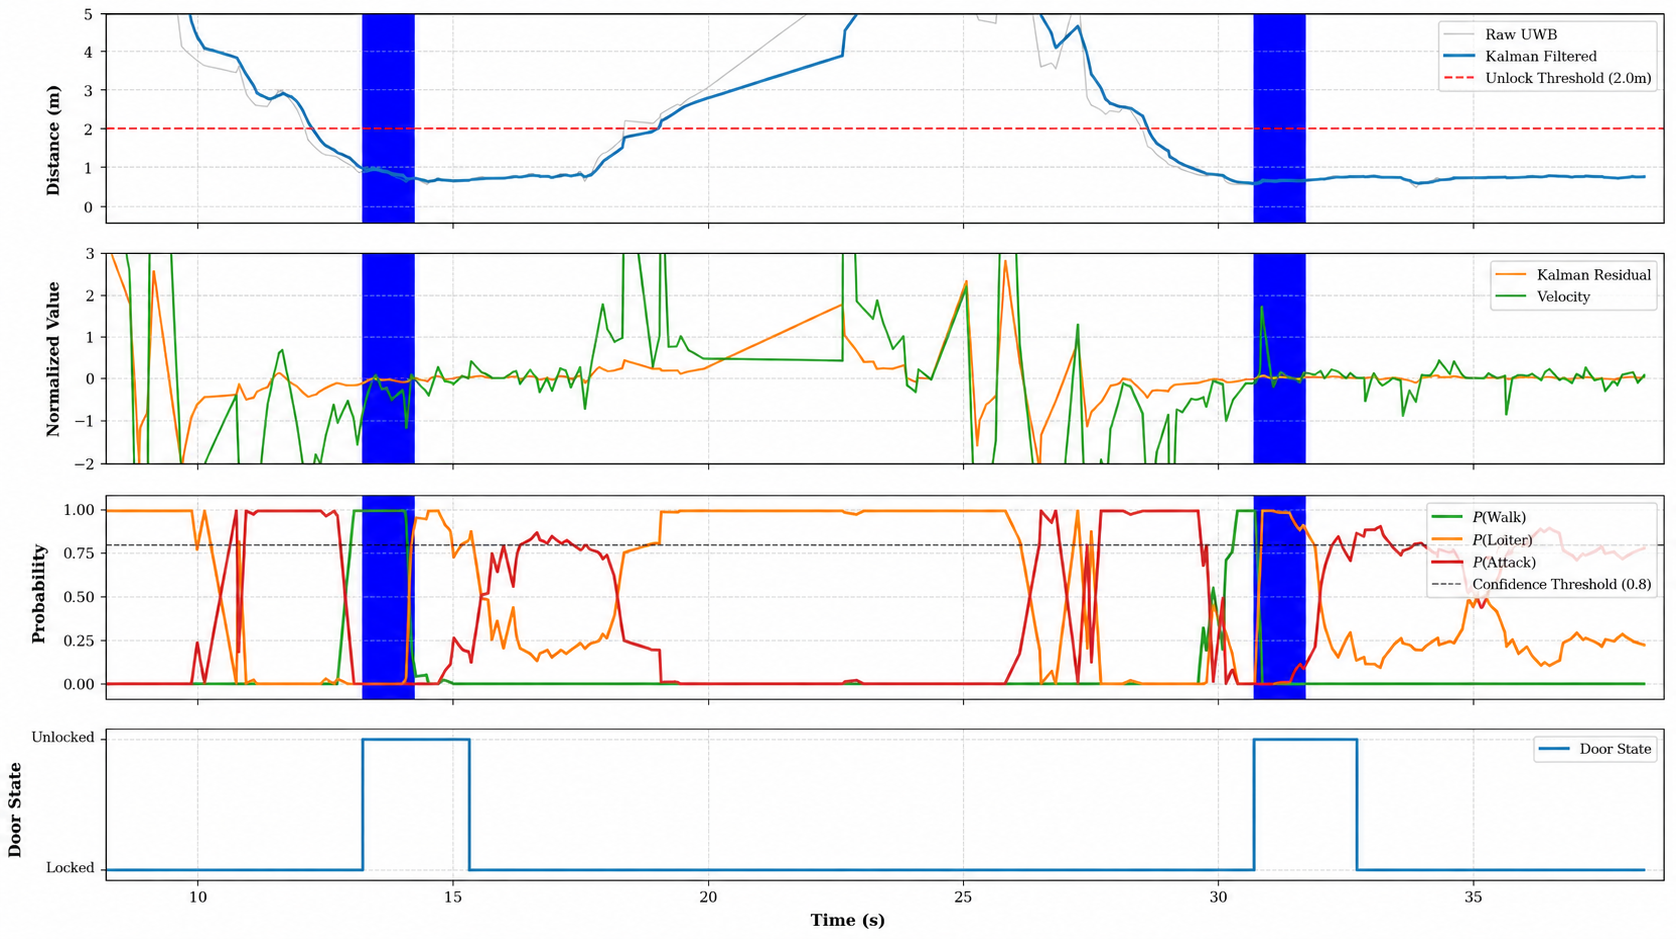
\includegraphics[width=0.9\textwidth]{image/LSTM/normal_behavior.png} % Thay bằng đường dẫn ảnh Walk/Loiter của em
        \caption{Đồ thị phân tích hành vi bình thường: Lảng vảng (Loiter) và Tiếp cận (Walk)}
        \label{fig:normal_behavior}
    \end{figure}

    \textbf{Kịch bản 1: Hành vi tự nhiên (Hình \ref{fig:normal_behavior})}
    \begin{itemize}
        \item \textit{Giai đoạn Lảng vảng:} Người dùng di chuyển quanh ranh giới 2m. Đồ thị Đặc trưng động học (Normalize value) cho thấy vận tốc (đường màu xanh lá) dao động liên tục (tiến và lùi), trong khi thặng dư (đường màu cam) rất nhỏ do di chuyển thực tế. Ngay lập tức, AI phản hồi bằng cách đẩy xác suất P(Loiter) lên mức cao (khoảng 0.8 đến 0.9), đồng thời đè P(Walk) xuống mức thấp, đảm bảo rơ-le cửa không bị kích hoạt sai.
        \item \textit{Giai đoạn Tiếp cận:} Khoảng cách giảm mượt mà và ổn định xuống dưới ngưỡng 2m. Quỹ đạo này tạo ra một vector vận tốc âm đều đặn. Mô hình AI lập tức nhận diện đúng ý định, đẩy xác suất P(Walk) vọt lên gần 1.0 và duy trì liên tục qua nhiều khung hình, kích hoạt cơ chế đồng thuận để mở cửa.
    \end{itemize}

    \begin{figure}[H]
        \centering
        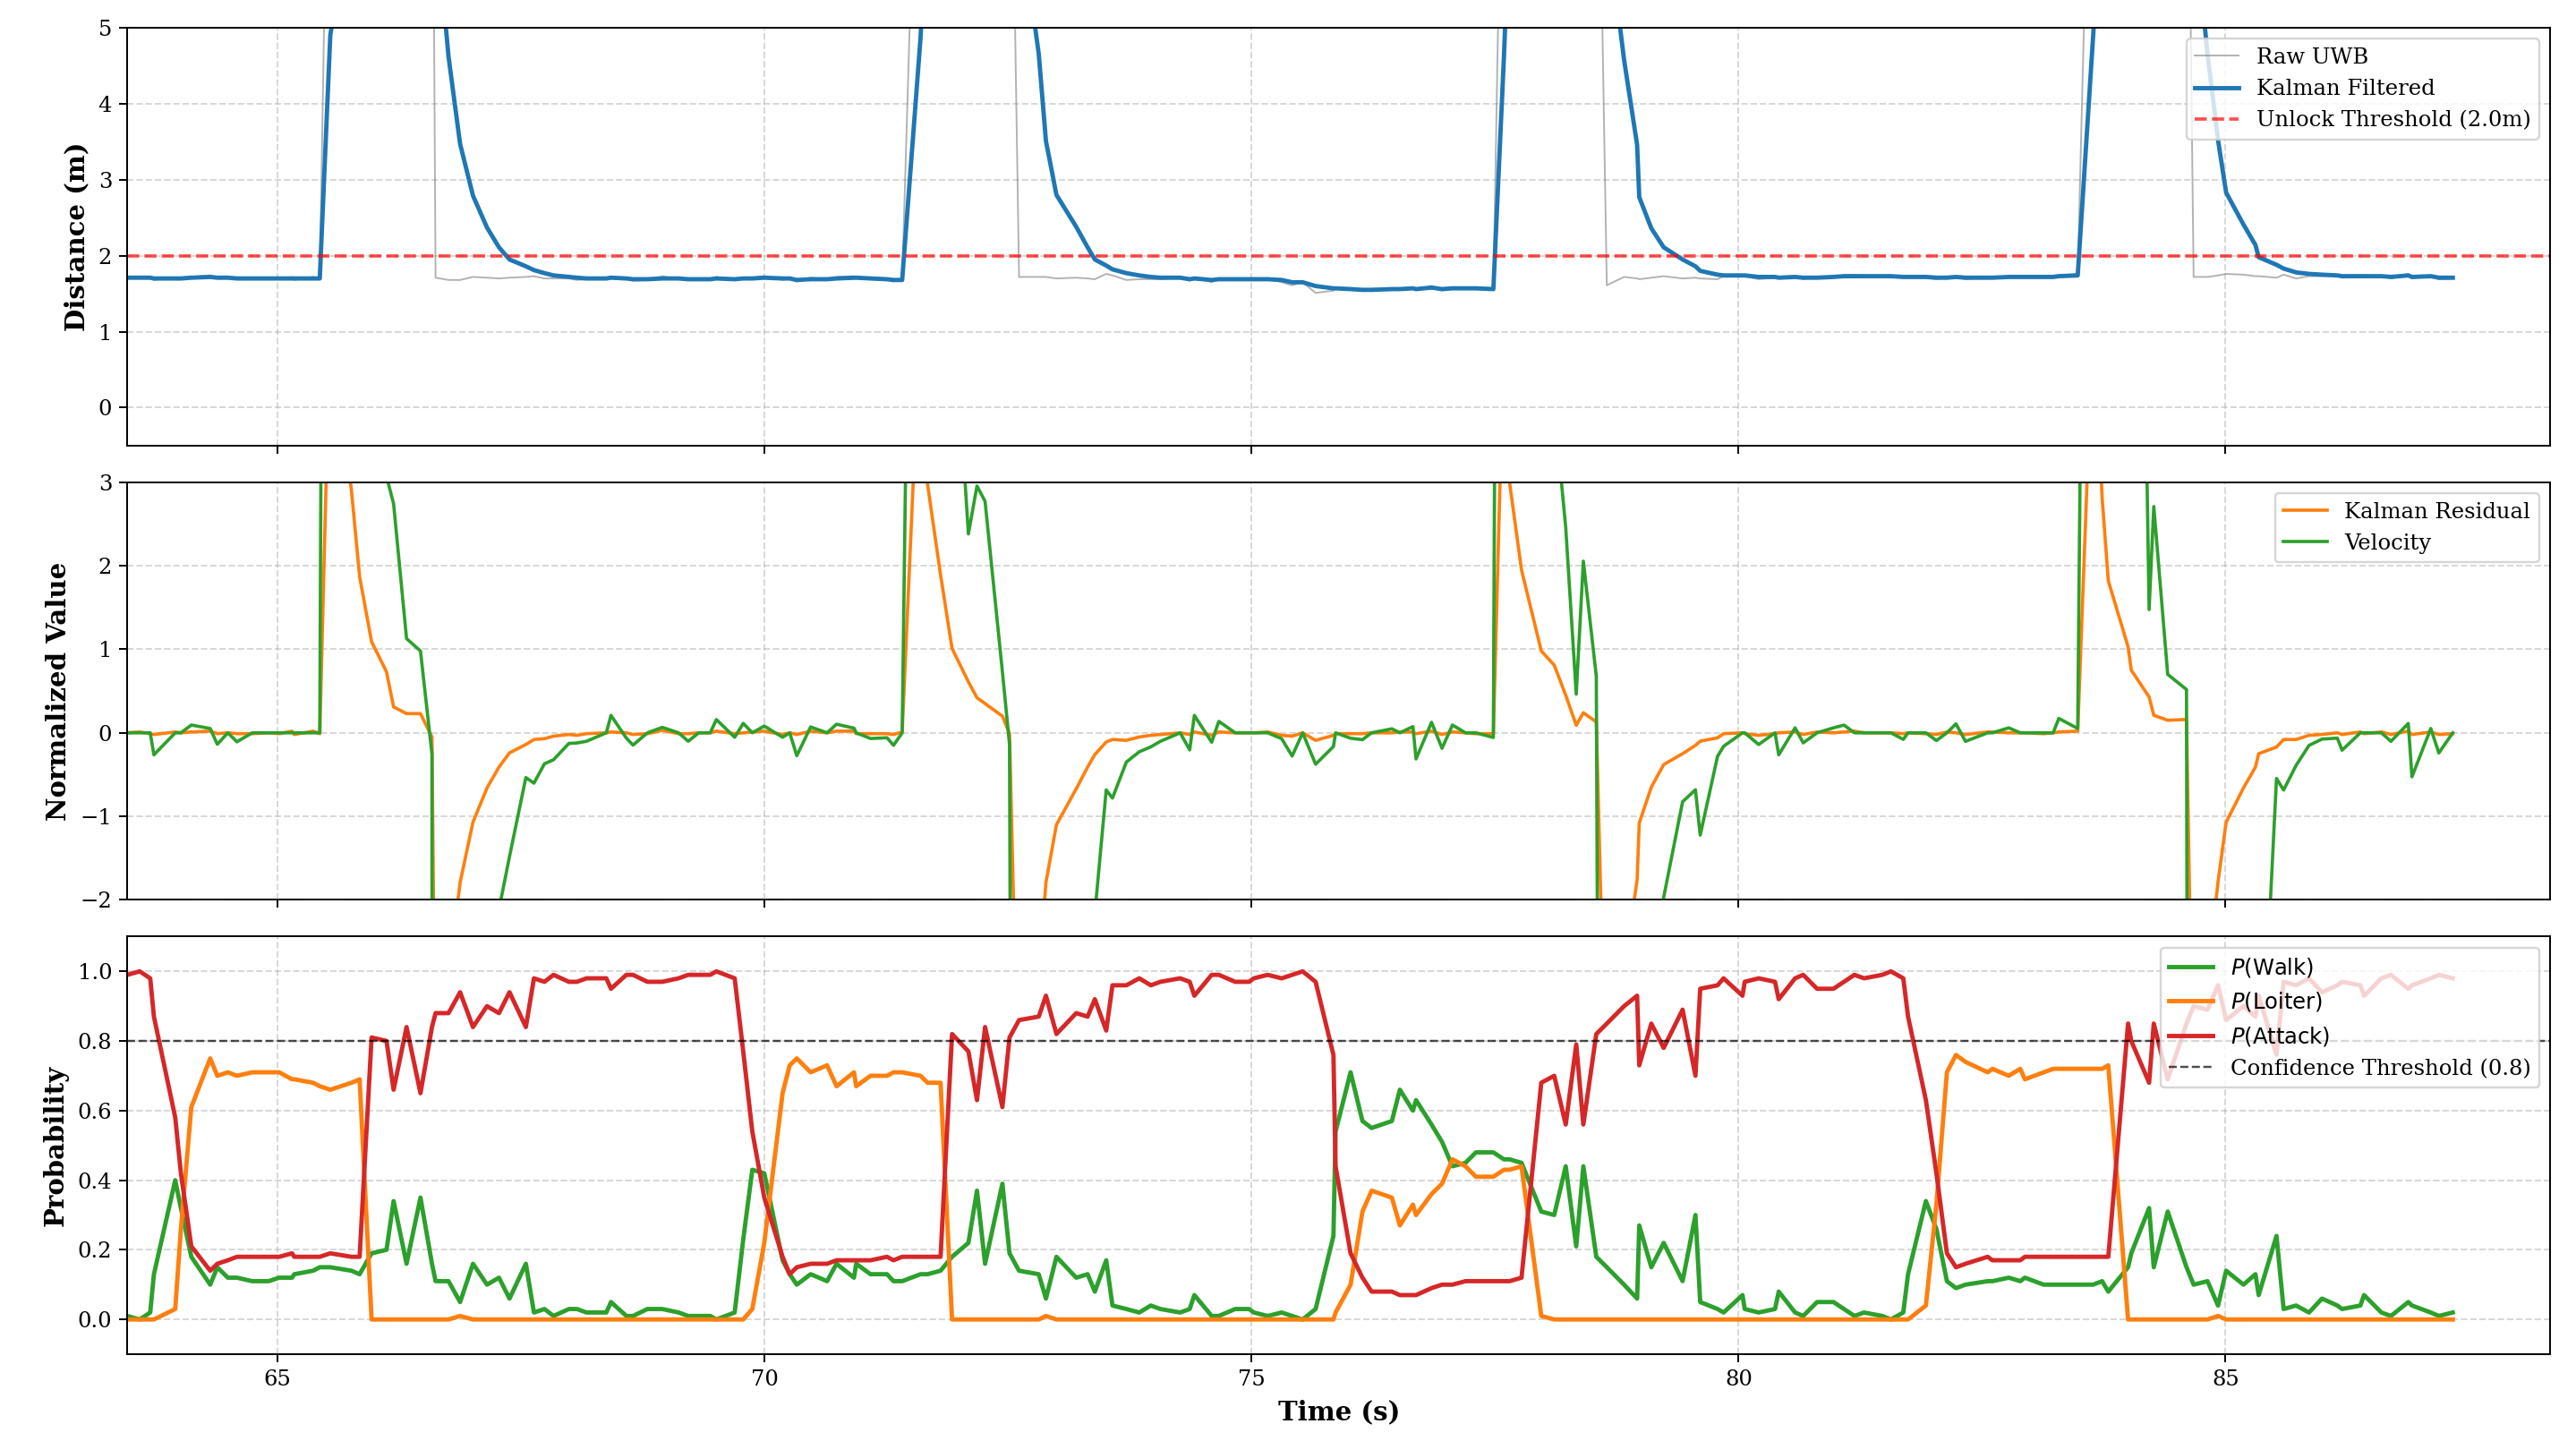
\includegraphics[width=0.9\textwidth]{image/LSTM/relay_attack.png} % Thay bằng đường dẫn ảnh Relay Attack của em
        \caption{Đồ thị phân tích kịch bản Tấn công tiếp sóng (Relay Attack)}
        \label{fig:relay_atk}
    \end{figure}

    \textbf{Kịch bản 2: Tấn công tiếp sóng giả mạo (Hình \ref{fig:relay_atk})}
    \begin{itemize}
        \item Đây là kịch bản phô diễn sức mạnh phòng thủ của hệ thống. Kẻ tấn công giả mạo tín hiệu, khiến khoảng cách thô (đường nét mờ ở đồ thị trên cùng) đột ngột rớt từ mức 5m xuống dưới 2m theo hình bậc thang.
        \item Nếu chỉ dùng if-else truyền thống, cửa sẽ mở ngay lập tức. Tuy nhiên, nhờ quán tính của bộ lọc Kalman, quỹ đạo bị trễ lại, tạo ra một sự sai lệch khổng lồ. Điều này được thể hiện rõ qua các cú giật cực lớn của đường Thặng dư (Residual - màu cam) ở đồ thị giữa.
        \item Khối 1D-CNN ngay lập tức bắt được đặc trưng dị thường này. Ở đồ thị dưới cùng, xác suất P(Attack) (đường màu đỏ) vọt lên mức gần 1.0 mỗi khi xuất hiện spike, trong khi P(Walk) bị dập tắt hoàn toàn. Hệ thống cưỡng bức trạng thái khóa an toàn, ngăn chặn triệt để cuộc tấn công.
    \end{itemize}
\end{itemize}



%-------------------------------------------------------------------------------------------------------------


\section{Thành tựu nghiên cứu và Công bố khoa học}

Một trong những kết quả nổi bật nhất của đề tài là việc đúc kết các nghiên cứu lý thuyết và thực nghiệm thành một công trình khoa học hoàn chỉnh. Bài báo mang tựa đề \textit{"Beyond Relay Attacks: A Cross-Layer and Robustness Evaluation of CCC Digital Key Systems Utilizing NFC, BLE, and UWB"} đã chính thức được chấp nhận báo cáo tại Hội nghị Quốc tế IAAA 2026 (The 2nd International Conference on Intelligent Aerial Access and Applications). Website chính thức của hội nghị: \url{https://cse.hcmut.edu.vn/iaaa2026/}

Đặc biệt, bài báo đã vượt qua quá trình bình duyệt (Peer-review) khắt khe và được chọn xuất bản trong chuỗi kỷ yếu danh giá \textbf{Lecture Notes in Networks and Systems (LNNS)} của nhà xuất bản \textbf{Springer}, được lập chỉ mục bởi \textbf{SCOPUS}. 

\begin{figure}[H]
    \centering
    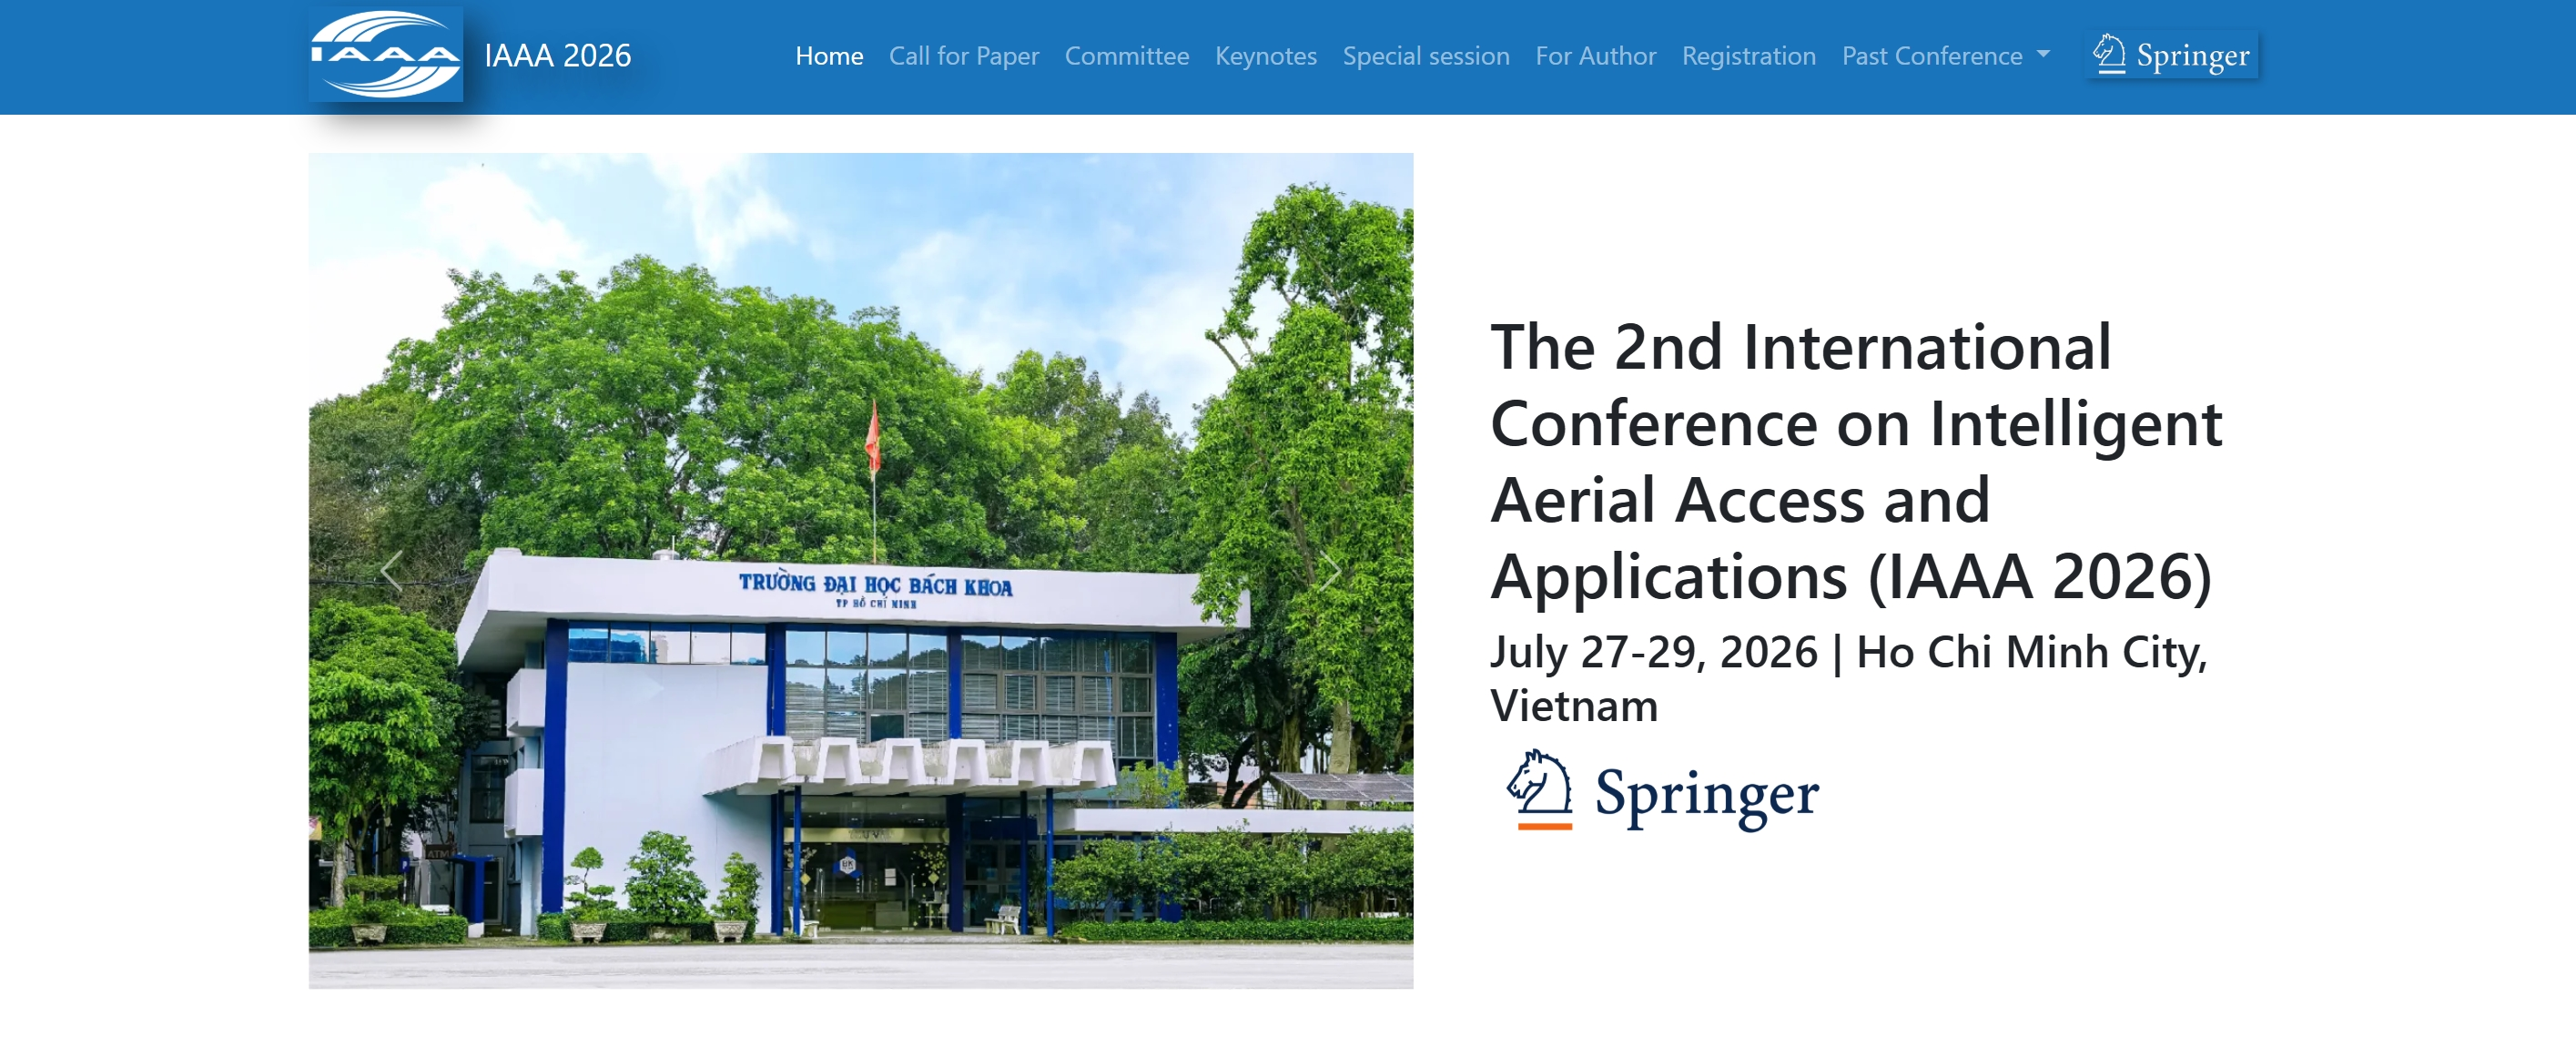
\includegraphics[width=\linewidth]{image/achievements/IAAA.jpeg}
    \caption{Hội nghị Quốc tế IAAA 2026 tổ chức tại trường ĐH Bách Khoa}
    \label{fig:iaaa_website}
\end{figure}

\begin{figure}[H]
    \centering
    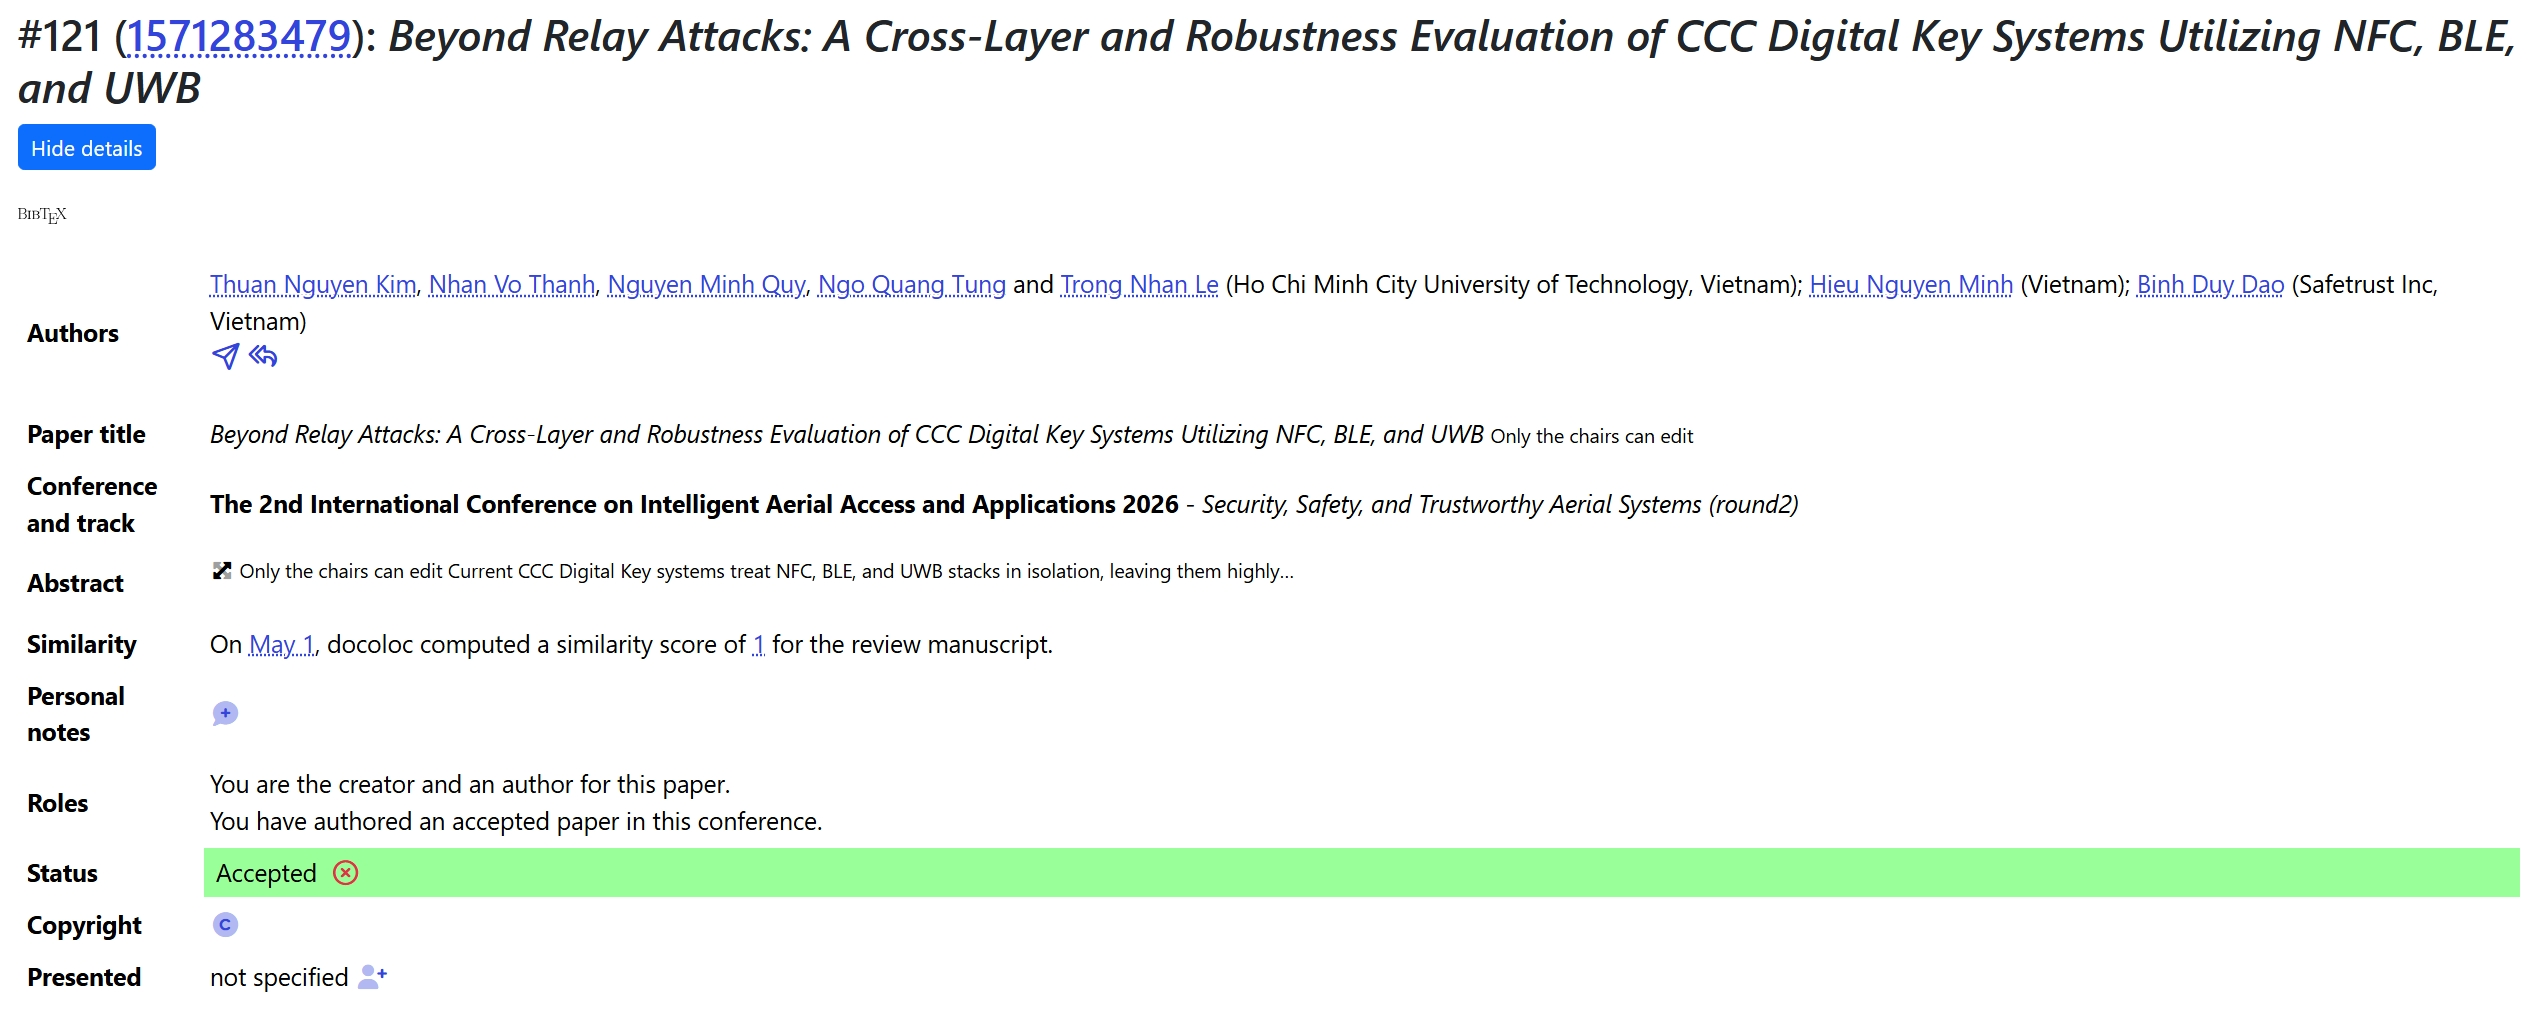
\includegraphics[width=\linewidth]{image/achievements/paper_accepted.jpeg}
    \caption{Minh chứng bài báo được chấp nhận (Accepted) trên hệ thống EDAS}
    \label{fig:paper_accepted}
\end{figure}


Dựa trên các nhận xét từ Hội đồng phản biện quốc tế (Reviewers's Comments), công trình của nhóm được đánh giá cao ở các khía cạnh sau:
\begin{itemize}
    \item \textbf{Tính thực tiễn và Kiến trúc phần cứng:} Hội đồng đánh giá cao việc nhóm sử dụng các phần cứng thương mại (Commodity hardware như ESP32-S3 và vi mạch DWM3000) thay vì chỉ mô phỏng lý thuyết. Kiến trúc bảo mật đa lớp chéo (Cross-Layer Security) kết hợp máy trạng thái FreeRTOS được nhận định là những "lựa chọn kỹ thuật hợp lý" (reasonable engineering choices) để liên kết chặt chẽ quá trình xác thực và đo lường khoảng cách.
    \item \textbf{Khả năng chống tấn công giả mạo (Relay Attack Defense):} Mô hình lai (Hybrid) kết hợp Bộ lọc Kalman và mạng LSTM được hội đồng công nhận là một thiết kế có tính thuyết phục cao (plausible design). Thuật toán không chỉ giới hạn kẻ tấn công ở không gian vật lý mà còn đưa hệ thống về trạng thái khóa an toàn (Fail-closed state) khi phát hiện dấu hiệu bất thường.
    \item \textbf{Đóng góp về thuật toán và chi phí:} Nghiên cứu đã chứng minh khả năng đạt được độ bảo mật cao chống lại các cuộc tấn công tiếp sóng chỉ với kiến trúc UWB đơn mỏ neo (Single-anchor), qua đó loại bỏ hoàn toàn rào cản về chi phí cao và sự phức tạp trong đồng bộ hóa của các hệ thống UWB đa mỏ neo (TDOA) truyền thống.
\end{itemize}

Việc công trình được cộng đồng học thuật quốc tế công nhận không chỉ khẳng định tính đúng đắn và cấp thiết của đề tài, mà còn là minh chứng cho năng lực nghiên cứu, phân tích và triển khai thực nghiệm của sinh viên trong việc giải quyết các bài toán an ninh phức tạp trên hệ thống nhúng ô tô hiện đại.

%-------------------------------------------------------------------------------------------------------------


\newpage
\chapter{\MakeUppercase{KẾT LUẬN VÀ ĐỊNH HƯỚNG PHÁT TRIỂN}}

Đồ án đã hoàn thành đầy đủ các mục tiêu nghiên cứu và thực nghiệm đề ra. Thông qua quá trình nghiên cứu lý thuyết, thiết kế kiến trúc và triển khai thực tế trên nền tảng hệ thống nhúng, nhóm nghiên cứu xin rút ra các kết luận tổng quát như sau:

\begin{enumerate}
    \item \textbf{Về mặt kiến trúc và giao thức:} Đồ án đã hiện thực hóa thành công mô hình bảo mật đa giao thức \textit{Tri-Radio} (NFC, BLE, UWB) bám sát đặc tả kỹ thuật của liên minh CCC Digital Key Release 3. Việc kết hợp chặt chẽ giữa cơ sở hạ tầng xác thực mật mã bất đối xứng (ECDSA/ECDH) và kỹ thuật đo đạc khoảng cách vật lý an toàn bằng sóng UWB đã tạo ra một "hàng rào" bảo mật đa lớp, giải quyết triệt để các rủi ro của hệ thống chìa khóa thông minh truyền thống.

    \item \textbf{Về mặt kỹ thuật nhúng và hiệu năng:} Hệ thống đã chứng minh tính khả thi khi vận hành ổn định các giao thức mật mã phức tạp và xử lý tín hiệu thời gian thực trên vi điều khiển ESP32-S3 dưới sự quản lý của hệ điều hành FreeRTOS. Các chỉ số hiệu năng thực tế, bao gồm độ trễ giao dịch toàn trình ($\approx 1.5$s) và độ trễ bàn giao kết nối ($\approx 630$ms), đều nằm trong ngưỡng đáp ứng tiêu chuẩn công nghiệp, mang lại trải nghiệm liền mạch cho người dùng.

    \item \textbf{Về điểm đột phá Trí tuệ nhân tạo (TinyML, đang hiện thực):} Điểm sáng tạo của đề tài là việc vượt ra khỏi các thuật toán so sánh ngưỡng (Rule-based) đơn thuần để nhúng mô hình học máy (mạng tích chập 1D - Conv1D) trực tiếp lên thiết bị biên nhằm nhận diện ý định hành vi. Kiến trúc định hướng ở giai đoạn 2 phân loại quỹ đạo $(x, y, v_x, v_y)$ thành bốn lớp ý định (Approach, Seated, Leave, Passing) và đóng vai trò cổng (gate) cho quyết định truy cập tất định, hướng tới nâng cấp hệ thống từ mức đo lường thụ động sang nhận thức thông minh.

    \item \textbf{Về giá trị thực tiễn và khoa học:} Đồ án là minh chứng cho việc làm chủ công nghệ xuyên suốt từ tầng vật lý (Physical Layer) đến tầng ứng dụng (Application Layer). Sự kết hợp giữa bộ lọc Kalman truyền thống và học máy hiện đại mở ra hướng tiếp cận khả thi và tối ưu chi phí cho các hệ thống an ninh ô tô thế hệ mới.
\end{enumerate}

Tóm lại, hệ thống Smart Car Access được phát triển trong đồ án là một giải pháp mang tính toàn diện, hội đủ các yếu tố: an ninh mật mã, ổn định phần cứng và thông minh hóa phần mềm. Đây là tiền đề quan trọng để phát triển các ứng dụng bảo mật ô tô hướng tới sự tiện nghi và an toàn tuyệt đối trong kỷ nguyên xe điện và xe tự hành.

\section*{Hạn chế của đề tài}
\addcontentsline{toc}{section}{Hạn chế của đề tài}

Mặc dù hệ thống đã hiện thực hóa thành công luồng truy cập PKE dựa trên kiến trúc Tri-Radio tuân thủ tiêu chuẩn CCC, đồ án vẫn còn một số rào cản nhất định do giới hạn về mặt thời gian, chi phí và tài nguyên phần cứng trong môi trường nghiên cứu học thuật.

\begin{itemize}
    \item \textbf{Giới hạn về nền tảng phần cứng và định vị không gian (Spatial Resolution):}
    \begin{itemize}
        \item Hệ thống hiện tại sử dụng vi điều khiển đa dụng ESP32-S3. Mặc dù có hiệu năng xử lý tốt, đây chưa phải là dòng vi điều khiển đạt chuẩn ô tô (Automotive-Grade MCU) và chưa đáp ứng các tiêu chuẩn an toàn chức năng khắt khe như ISO 26262 hay kiến trúc phần mềm AUTOSAR.
        \item Về mặt định vị, hệ thống giai đoạn hai đã nâng cấp từ đo khoảng cách đơn mỏ neo (1D) lên định vị đa mỏ neo với ba mỏ neo UWB, cho phép giải tọa độ phẳng $(x, y)$ của người dùng thông qua Trilateration kết hợp bộ lọc Kalman. Tuy nhiên, các mỏ neo hiện được kết nối với xe gián tiếp qua một cầu nối PC (mang tính nghiên cứu, chưa phải cấu trúc liên kết sản xuất), tọa độ mỏ neo được cố định trong mã nguồn và hệ thống chưa khai thác tham số Góc đến (Angle of Arrival - AoA). Do đó, định vị mới dừng ở mặt phẳng hai chiều và chưa đủ cơ sở để phân biệt các vùng kích hoạt cục bộ một cách tinh tế (ví dụ: mở cốp khi người dùng đứng chính giữa sau đuôi xe so với lệch một bên).
    \end{itemize}

    \item \textbf{Mức độ triển khai Hạ tầng khóa công khai (PKI):}
    \begin{itemize}
        \item Một hệ thống thương mại chuẩn CCC yêu cầu phải có Hạ tầng quản lý chứng chỉ số (PKI) hoàn chỉnh. Trong phạm vi đồ án, quy trình cấp quyền (Provisioning) mới dừng ở mức mô phỏng cục bộ thông qua thẻ vật lý (Master Card) thay vì xác thực đám mây thông qua các máy chủ OEM chuyên dụng.
    \end{itemize}

    \item \textbf{Tiến độ nhúng mô hình học máy (TinyML, đang hiện thực):}
    \begin{itemize}
        \item Hệ thống đã trích xuất thành công đặc trưng vật lý và tối ưu hóa quỹ đạo bằng bộ lọc Kalman hai chiều (EKF), tạo chuỗi trạng thái $(x, y, v_x, v_y)$ chất lượng cao làm đầu vào cho mô hình. Mô hình nhận diện ý định hành vi (Conv1D/TFLM) hiện đang trong quá trình thu thập dữ liệu, huấn luyện và nhúng lên ESP32-S3. Do đó, để đảm bảo tính an toàn cơ học tuyệt đối, logic ra quyết định mở cửa hiện tại vẫn ưu tiên sử dụng thuật toán Hysteresis kết hợp bộ lọc Kalman làm cốt lõi tất định.
    \end{itemize}

    \item \textbf{Độ phủ của dữ liệu huấn luyện (Model Coverage):}
    \begin{itemize}
        \item Dù mô hình phân loại hành vi đạt độ chính xác khá tốt, bộ dữ liệu hiện tại chưa bao quát hết mọi kịch bản môi trường phức tạp (như bãi đỗ xe có nhiều vật cản kim loại gây nhiễu đa đường mạnh). Để đạt độ tin cậy cấp độ thương mại ($>95\%$), hệ thống cần thu thập lượng dữ liệu đa dạng hơn từ nhiều mẫu hành vi và thiết bị di động khác nhau.
    \end{itemize}
\end{itemize}

\section*{Định hướng phát triển}
\addcontentsline{toc}{section}{Định hướng phát triển}

Từ những kết quả và hạn chế đã phân tích, nhóm nghiên cứu đề xuất các hướng phát triển tiếp theo nhằm hoàn thiện và nâng cao tính ứng dụng của hệ thống:

\begin{enumerate}
    \item \textbf{Nâng cấp định vị không gian đa chiều (AoA và nhúng trực tiếp):} Tích hợp mảng ăng-ten (Antenna Array) nhằm khai thác tham số Góc đến, đồng thời nhúng các bộ thu phát UWB trực tiếp lên ECU để loại bỏ cầu nối PC. Việc kết hợp giữa Khoảng cách (nhiều mỏ neo) và Góc sẽ cho phép hệ thống xác định chính xác vị trí người dùng trong không gian, hỗ trợ các tính năng cao cấp như "Welcome Light" hay "Smart Trunk" (Mở cốp thông minh) theo vùng (geofencing).
    
    \item \textbf{Tối ưu hóa độ chính xác mô hình học máy:} Áp dụng các kỹ thuật Tăng cường dữ liệu (Data Augmentation) và thử nghiệm các kiến trúc lai (Hybrid CNN-LSTM) phù hợp với tài nguyên thiết bị biên. Mục tiêu là tối đa hóa tỷ lệ nhận diện hành vi và giảm thiểu triệt để sai số định vị trong môi trường nhiễu sóng mạnh.
    
    \item \textbf{Tiêu chuẩn hóa phần cứng và hệ sinh thái:} Chuyển đổi kiến trúc trung tâm sang các dòng vi điều khiển đạt chuẩn Automotive (như NXP S32K) đáp ứng tiêu chuẩn an toàn ASIL-B. Đồng thời, nghiên cứu tích hợp hệ thống lên hệ điều hành iOS thông qua nền tảng Apple CarKey API.
    
    \item \textbf{Hoàn thiện hạ tầng PKI trên nền tảng Đám mây:} Xây dựng máy chủ mô phỏng Vehicle OEM để quản lý vòng đời khóa kỹ thuật số, từ đó hiện thực hóa quy trình đăng ký chìa khóa (Owner Provisioning) và chia sẻ chìa khóa (Key Sharing) từ xa an toàn theo đúng đặc tả kỹ thuật của CCC.
\end{enumerate}

\addcontentsline{toc}{chapter}{DANH MỤC TÀI LIỆU THAM KHẢO}
\newpage

\begin{thebibliography}{99}

\bibitem{axelson_serial}
Axelson, J. (2007). \textit{Serial Port Complete: The Developer's Guide} (2nd ed.). Lakeview Research.

\bibitem{autosar}
AUTOSAR Partners. (2017). \textit{AUTOSAR Layered Software Architecture} (Version 4.3.1).

\bibitem{arduinojson}
Blanchon, B. (2025). \textit{ArduinoJson: Efficient JSON serialization for embedded C++}. [Online]. Available: https://arduinojson.org.

\bibitem{bluetooth40}
Bluetooth SIG. (2010). \textit{Bluetooth Core Specification Version 4.0}. Bluetooth Special Interest Group. Retrieved from https://www.bluetooth.com/

\bibitem{ble_core}
Bluetooth SIG. (2016). \textit{Bluetooth Core Specification Version 5.0}. Bluetooth Special Interest Group.
\bibitem{miller1985use} V. S. Miller, ``Use of Elliptic Curves in Cryptography,'' in \textit{Advances in Cryptology --- CRYPTO '85}, vol. 218, Lecture Notes in Computer Science, pp. 417--426, Springer, 1985. DOI: 10.1007/3-540-39799-X\_31

\bibitem{koblitz1987elliptic} N. Koblitz, ``Elliptic Curve Cryptosystems,'' \textit{Mathematics of Computation}, vol. 48, no. 177, pp. 203--209, 1987. DOI: 10.1090/S0025-5718-1987-0866109-5

\bibitem{fips186} National Institute of Standards and Technology, \textit{Digital Signature Standard (DSS)}, Federal Information Processing Standards Publication 186-4, U.S. Department of Commerce, July 2013. Available: \url{https://doi.org/10.6028/NIST.FIPS.186-4}

\bibitem{nist80056a} National Institute of Standards and Technology, \textit{Recommendation for Pair-Wise Key-Establishment Schemes Using Discrete Logarithm Cryptography}, NIST Special Publication 800-56A Revision 3, U.S. Department of Commerce, April 2018. Available: \url{https://doi.org/10.6028/NIST.SP.800-56Ar3}
\bibitem{nist80038d} National Institute of Standards and Technology, \textit{Recommendation for Block Cipher Modes of Operation: Galois/Counter Mode (GCM) and GMAC}, NIST Special Publication 800-38D, U.S. Department of Commerce, November 2007. Available: \url{https://doi.org/10.6028/NIST.SP.800-38D}
\bibitem{bharadwaj2020accurate}
Bharadwaj, R., Swaisaenyakorn, S., Parini, C. G., Batchelor, J. C., \& Koul, A. (2020). Localization of wearable ultrawideband antennas for motion capture applications. \textit{IEEE Antennas and Wireless Propagation Letters}, 13, 507-510. DOI: 10.1109/LAWP.2014.2313133

\bibitem{coskun2013professional}
Coskun, V., Ozdenizci, B., \& Ok, K. (2013). \textit{Professional NFC Application Development for Android}. John Wiley \& Sons.

\bibitem{daemen2002design}
Daemen, J., \& Rijmen, V. (2002). \textit{The design of Rijndael: AES-the advanced encryption standard}. Springer Science \& Business Media.

\bibitem{decawave2017}
DecaWave (Qorvo). (2017). \textit{DW1000 User Manual Version 2.18}. Qorvo, Inc. Retrieved from https://www.qorvo.com/products/p/DW1000

\bibitem{esp32s3}
Espressif Systems. (2022). \textit{ESP32-S3 Series Datasheet, Version 1.1}.

\bibitem{espidf_nvs}
Espressif Systems. (2024). \textit{ESP-IDF Programming Guide: Non-Volatile Storage Library}.

\bibitem{fcc2002}
Federal Communications Commission. (2002). \textit{Revision of Part 15 of the Commission's Rules Regarding Ultra-Wideband Transmission Systems, First Report and Order}. FCC 02-48, ET Docket No. 98-153. Washington, DC.

\bibitem{finkenzeller2010rfid}
Finkenzeller, K. (2010). \textit{RFID Handbook: Fundamentals and Applications in Contactless Smart Cards, Radio Frequency Identification and Near-Field Communication} (3rd ed.). John Wiley \& Sons.

\bibitem{francillon2011relay}
Francillon, A., Danev, B., \& Capkun, S. (2011). Relay attacks on passive keyless entry and start systems in modern cars. In \textit{Proceedings of the Network and Distributed System Security Symposium (NDSS)}. San Diego, CA.

\bibitem{ghavami2007ultra}
Ghavami, M., Michael, L. B., \& Kohno, R. (2007). \textit{Ultra Wideband Signals and Systems in Communication Engineering}. John Wiley \& Sons.

\bibitem{gomez2012overview}
Gomez, C., Oller, J., \& Paradells, J. (2012). Overview and evaluation of bluetooth low energy: An emerging low-power wireless technology. \textit{Sensors}, 12(9), 11734-11753. DOI: 10.3390/s120911734

\bibitem{mckinsey2023}
McKinsey \& Company. (2023). \textit{Outlook on the automotive software and electronics market through 2030}. McKinsey Center for Future Mobility. [Online]. Available: \url{https://www.mckinsey.com/features/mckinsey-center-for-future-mobility/our-insights/mapping-the-automotive-software-and-electronics-landscape-2024}

\bibitem{flutter_docs}
Google. (2025). \textit{Flutter SDK Documentation}. [Online]. Available: https://docs.flutter.dev.

\bibitem{firebase_docs}
Google. (2025). \textit{Firebase Documentation: Authentication and Cloud Firestore}. [Online]. Available: https://firebase.google.com/docs.

\bibitem{android_security}
Google Developers. (2025). \textit{Android Keystore System and Host-based Card Emulation (HCE) Documentation}. [Online]. Available: https://developer.android.com/training/articles/keystore.

\bibitem{haataja2008bluetooth}
Haataja, K., \& Toivanen, P. (2008). Two practical man-in-the-middle attacks on Bluetooth secure simple pairing and countermeasures. \textit{IEEE Transactions on Wireless Communications}, 9(1), 384-392.

\bibitem{nimble_arduino}
h2zero. (2024). \textit{NimBLE-Arduino: A Bluetooth Low Energy library for ESP32}. GitHub Repository.

\bibitem{haselsteiner2006security}
Haselsteiner, E., \& Breitfuß, K. (2006). Security in near field communication (NFC). In \textit{Workshop on RFID Security} (RFIDSec 2006), Graz, Austria (pp. 12-14).

\bibitem{heydon2013bluetooth}
Heydon, R. (2013). \textit{Bluetooth Low Energy: The Developer's Handbook}. Prentice Hall. ISBN: 978-0132888363.

\bibitem{ieee802154}
IEEE 802.15.4a. (2007). \textit{IEEE Standard for Low-Rate Wireless Networks -- Amendment 1: Add Alternate PHYs}. IEEE.

\bibitem{ieee802154z}
IEEE 802.15.4z. (2020). \textit{IEEE Standard for Low-Rate Wireless Networks -- Amendment 1: Enhanced Ultra Wideband (UWB) Physical Layers (PHYs) and Associated Ranging Techniques}. Institute of Electrical and Electronics Engineers. DOI: 10.1109/IEEESTD.2020.9179124

\bibitem{iso14443}
ISO/IEC 14443. (2016). \textit{Identification cards -- Contactless integrated circuit cards -- Proximity cards}. International Organization for Standardization.

\bibitem{iso14443-2}
ISO/IEC 14443-4:2018. (2018). \textit{Identification cards -- Contactless integrated circuit cards -- Part 4: Transmission protocol}. International Organization for Standardization.

\bibitem{iso18092}
ISO/IEC 18092. (2013). \textit{Information technology -- Telecommunications and information exchange between systems -- Near Field Communication -- Interface and Protocol (NFCIP-1)}. International Organization for Standardization.

\bibitem{iso26262}
ISO 26262-1:2018. (2018). \textit{Road vehicles -- Functional safety}. International Organization for Standardization.

\bibitem{iso7816}
ISO/IEC 7816-4. (2020). \textit{Identification cards -- Integrated circuit cards -- Part 4: Organization, security and commands for interchange}. International Organization for Standardization/International Electrotechnical Commission.

\bibitem{iso7816-2}
ISO/IEC 7816-4:2020. (2020). \textit{Identification cards -- Integrated circuit cards -- Part 4: Organization, security and commands for interchange}. International Organization for Standardization.

\bibitem{jimenez2017survey}
Jiménez, A. R., \& Seco, F. (2017). Improving the accuracy of decawave's UWB MDEK1001 location system by gaining access to multiple ranges. \textit{Sensors}, 21(5), 1787. DOI: 10.3390/s21051787

\bibitem{joux2006authentication}
Joux, A. (2006). Authentication failures in NIST version of GCM. Retrieved from https://csrc.nist.gov/csrc/media/projects/block-cipher-techniques/documents/bcm/joux\_comments.pdf

\bibitem{rfc2104}
Krawczyk, H., Bellare, M., \& Canetti, R. (1997). HMAC: Keyed-Hashing for Message Authentication. \textit{RFC 2104}. DOI: 10.17487/RFC2104

\bibitem{rfc5869}
Krawczyk, H., \& Eronen, P. (2010). \textit{HMAC-based Extract-and-Expand Key Derivation Function (HKDF)}. RFC 5869, Internet Engineering Task Force.

\bibitem{lindell2009attacks}
Lindell, A. Y. (2009). Attacks on the pairing protocol of Bluetooth v2.1. In \textit{Black Hat USA}.

\bibitem{madlmayr2008nfc}
Madlmayr, G., Langer, J., Kantner, C., \& Scharinger, J. (2008). NFC devices: Security and privacy. In \textit{Third International Conference on Availability, Reliability and Security} (pp. 642-647). IEEE.

\bibitem{mulliner2009vulnerability}
Mulliner, C. (2009). Vulnerability analysis and attacks on NFC-enabled mobile phones. In \textit{International Conference on Availability, Reliability and Security} (pp. 695-700). IEEE.

\bibitem{fips186}
National Institute of Standards and Technology (NIST). (2013). \textit{FIPS PUB 186-4: Digital Signature Standard (DSS)}. U.S. Department of Commerce.

\bibitem{nist_ecdh}
National Institute of Standards and Technology (NIST). (2018). \textit{NIST SP 800-56A Rev. 3: Recommendation for Pair-Wise Key Establishment Schemes Using Discrete Logarithm Cryptography}.

\bibitem{fips197}
National Institute of Standards and Technology (NIST). (2001). \textit{FIPS PUB 197: Advanced Encryption Standard (AES)}.

\bibitem{fips198}
NIST. (2008). \textit{The Keyed-Hash Message Authentication Code (HMAC)}. FIPS PUB 198-1. U.S. Department of Commerce.

\bibitem{neirynck2016overview}
Neirynck, D., Luk, E., \& McLaughlin, M. (2016). An alternative double-sided two-way ranging method. In \textit{13th Workshop on Positioning, Navigation and Communications (WPNC)} (pp. 1-4). IEEE. DOI: 10.1109/WPNC.2016.7822844

\bibitem{nxp_pn532}
NXP Semiconductors. (2007). \textit{PN532/C1: Near Field Communication (NFC) controller - User Manual} (Rev. 3.2).

\bibitem{platformio_docs}
PlatformIO Labs. (2025). \textit{PlatformIO Documentation}. [Online]. Available: https://docs.platformio.org.

\bibitem{richards_arch}
Richards, M. (2015). \textit{Software Architecture Patterns}. O'Reilly Media, Inc.

\bibitem{ridolfi2018analysis}
Ridolfi, M., Van de Velde, S., Steendam, H., \& De Poorter, E. (2018). Analysis of the scalability of UWB indoor localization solutions for high user densities. \textit{Sensors}, 18(6), 1875. DOI: 10.3390/s18061875

\bibitem{roland2013software}
Roland, M., Langer, J., \& Scharinger, J. (2013). \textit{Applying relay attacks to Google Wallet}. In 5th International Workshop on Near Field Communication (NFC) (pp. 1-6). IEEE.

\bibitem{ryan2013bluetooth}
Ryan, M. (2013). Bluetooth: With low energy comes low security. In \textit{7th USENIX Workshop on Offensive Technologies (WOOT 13)}. USENIX Association.

\bibitem{fsm_book}
Samek, M. (2008). \textit{Practical UML Statecharts in C/C++: Event-Driven Programming for Embedded Systems} (2nd ed.). Newnes.

\bibitem{sidorenko2020accurate}
Sidorenko, J., Schatz, V., Scherer-Negenborn, N., Arens, M., \& Hugentobler, U. (2020). Decawave UWB clock drift correction and power self-calibration. \textit{Sensors}, 20(13), 3527. DOI: 10.3390/s20133527

\bibitem{townsend2014getting}
Townsend, K., Cufí, C., Akiba, \& Davidson, R. (2014). \textit{Getting Started with Bluetooth Low Energy: Tools and Techniques for Low-Power Networking}. O'Reilly Media. ISBN: 978-1491949511.

\bibitem{mbedtls_docs}
Trusted Firmware. (2025). \textit{Mbed TLS Documentation}. [Online]. Available: https://mbed-tls.readthedocs.io.

\bibitem{vama2023}
Vietnam Automobile Manufacturers' Association (VAMA). (2023). \textit{Vietnam Automobile Market Report 2023}. VAMA, Ho Chi Minh City, Vietnam. Available: \url{http://vama.org.vn}

\bibitem{wouters2021tesla}
Wouters, L., Marin, E., Ashur, T., Gierlichs, B., \& Preneel, B. (2021). Fast, Furious and Insecure: Passive Keyless Entry and Start Systems in Modern Supercars. \textit{IACR Transactions on Cryptographic Hardware and Embedded Systems}, 2021(3), 66-85. DOI: 10.46586/tches.v2021.i3.66-85

\bibitem{ccc_digikey3}
Car Connectivity Consortium. (2021). \textit{Digital Key Release 3.0: The Future of Vehicle Access}. White Paper. Beaverton, OR. Available: \url{https://carconnectivity.org}

\bibitem{nxp_ncj29d5}
NXP Semiconductors. (2019). \textit{NCJ29D5: Ultra-Wideband (UWB) IC for Automotive Applications}. Product Data Sheet. Eindhoven, Netherlands. Available: \url{https://www.nxp.com/docs/en/fact-sheet/NCJ29D5FS.pdf}

\bibitem{nxp_pn532}
NXP Semiconductors. (2007). \textit{PN532/C1: Near Field Communication (NFC) controller - User Manual} (Rev. 3.2). Document Number: 141520. Available: \url{https://www.nxp.com}
\end{thebibliography}


\newpage
\appendix
\chapter{\MakeUppercase{KHAI BÁO TRÁCH NHIỆM}}
Đồ án tốt nghiệp \textit{"Nghiên cứu và Phát triển hệ thống Định vị đa điểm (Multi-anchor) và Nhận diện ý định hành vi dựa trên TinyML cho giải pháp Smart Car Access"} được thực hiện bởi sinh viên \textbf{Võ Thành Nhân} (MSSV: 2111914). Khối lượng công việc được phân bổ dựa trên thế mạnh chuyên môn nhằm đảm bảo hiệu quả tích hợp hệ thống như sau:

\textbf{Võ Thành Nhân (MSSV: 2111914):} Chuyên trách toàn bộ hệ thống nhúng, trí tuệ nhân tạo (TinyML), ứng dụng di động và bảo mật giao thức CCC. Cụ thể, sinh viên đảm nhận lập trình hệ điều hành FreeRTOS trên ESP32-S3, thiết kế cầu nối PC thu thập dữ liệu từ ba mỏ neo UWB (DWM3001CDK), triển khai thuật toán định vị Trilateration và bộ lọc Kalman hai chiều (EKF) cùng khối quyết định truy cập hình học AccessController. Đồng thời, sinh viên phát triển ứng dụng Flutter thiết lập dịch vụ mô phỏng thẻ NFC (Android HCE), quản lý hạ tầng Firebase, triển khai luồng bắt tay mật mã Phase B (ECDH, ECDSA, HKDF-SHA256) và thiết kế chuẩn giao thức chuyển giao kết nối (Handoff) OOB từ kênh BLE sang UWB. Bên cạnh đó, sinh viên chịu trách nhiệm toàn bộ quy trình AI: thu thập dữ liệu, huấn luyện mạng học sâu (Conv1D/LSTM), lượng tử hóa và nhúng mô hình bằng TFLite Micro với cơ chế đồng thuận khung hình để chống tấn công tiếp sóng, đồng thời đảm nhận vai trò chính trong việc tham gia viết bài báo khoa học.

\textbf{Trách nhiệm chung:} Xuyên suốt dự án, sinh viên trực tiếp nghiên cứu tài liệu đặc tả FiRa/CCC, thực hiện đo đạc thực nghiệm vật lý (xác định sai số 24cm, kiểm thử độ trễ), tối ưu hóa tiêu thụ năng lượng phần cứng, tích hợp toàn diện hệ thống và tổng hợp số liệu để hoàn thiện báo cáo luận văn này.

\vspace{1cm}
\noindent \textit{Tôi xin cam đoan những khai báo trên là hoàn toàn đúng sự thật và phản ánh chính xác nỗ lực đóng góp của bản thân trong suốt quá trình thực hiện đồ án.}



% \newpage
% \thispagestyle{empty}
% \mbox{}

% \fancyhf{}
% \newpage
% 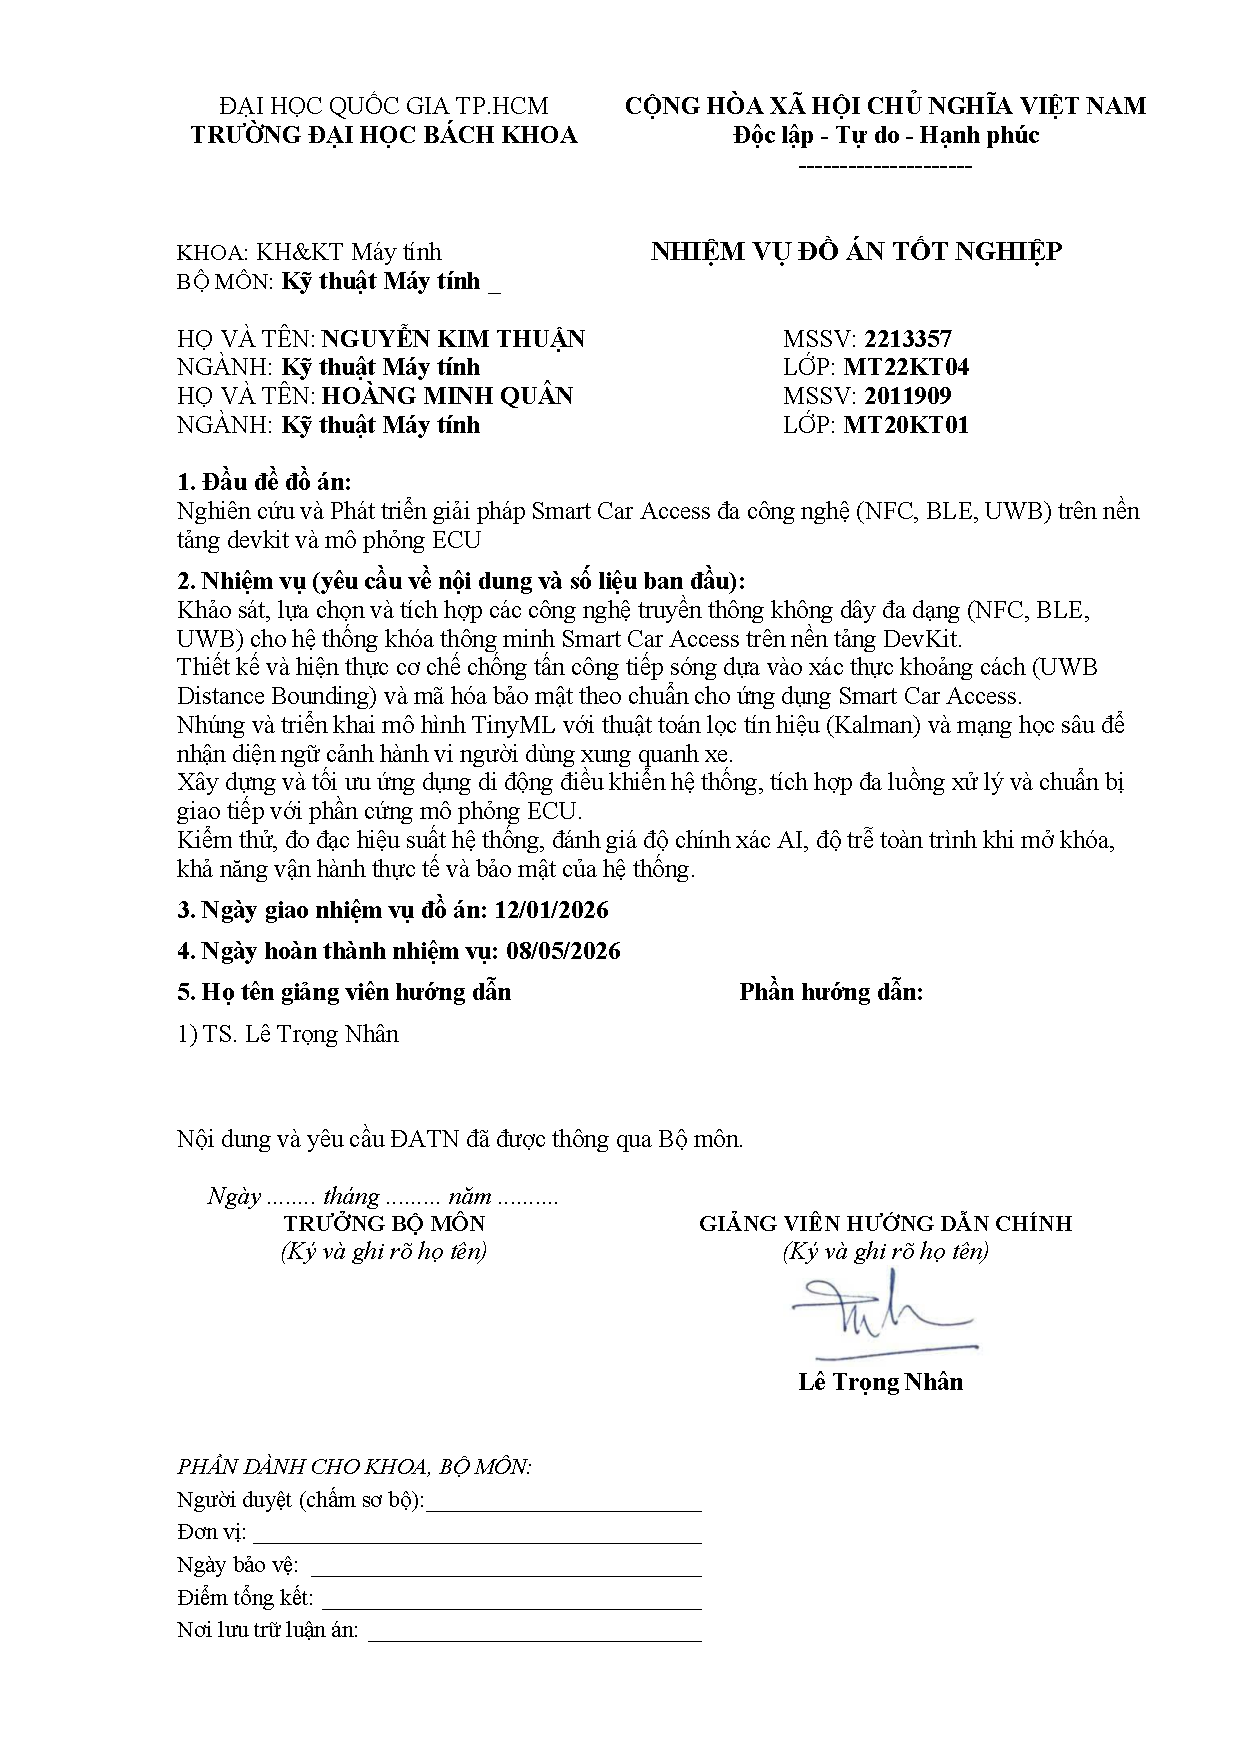
\includepdf[pages=1,pagecommand={},width=\paperwidth,height=\paperheight]{pdf files/Nv_signed.pdf}


% \newpage
% \thispagestyle{empty}
% \mbox{}
% \newpage

% 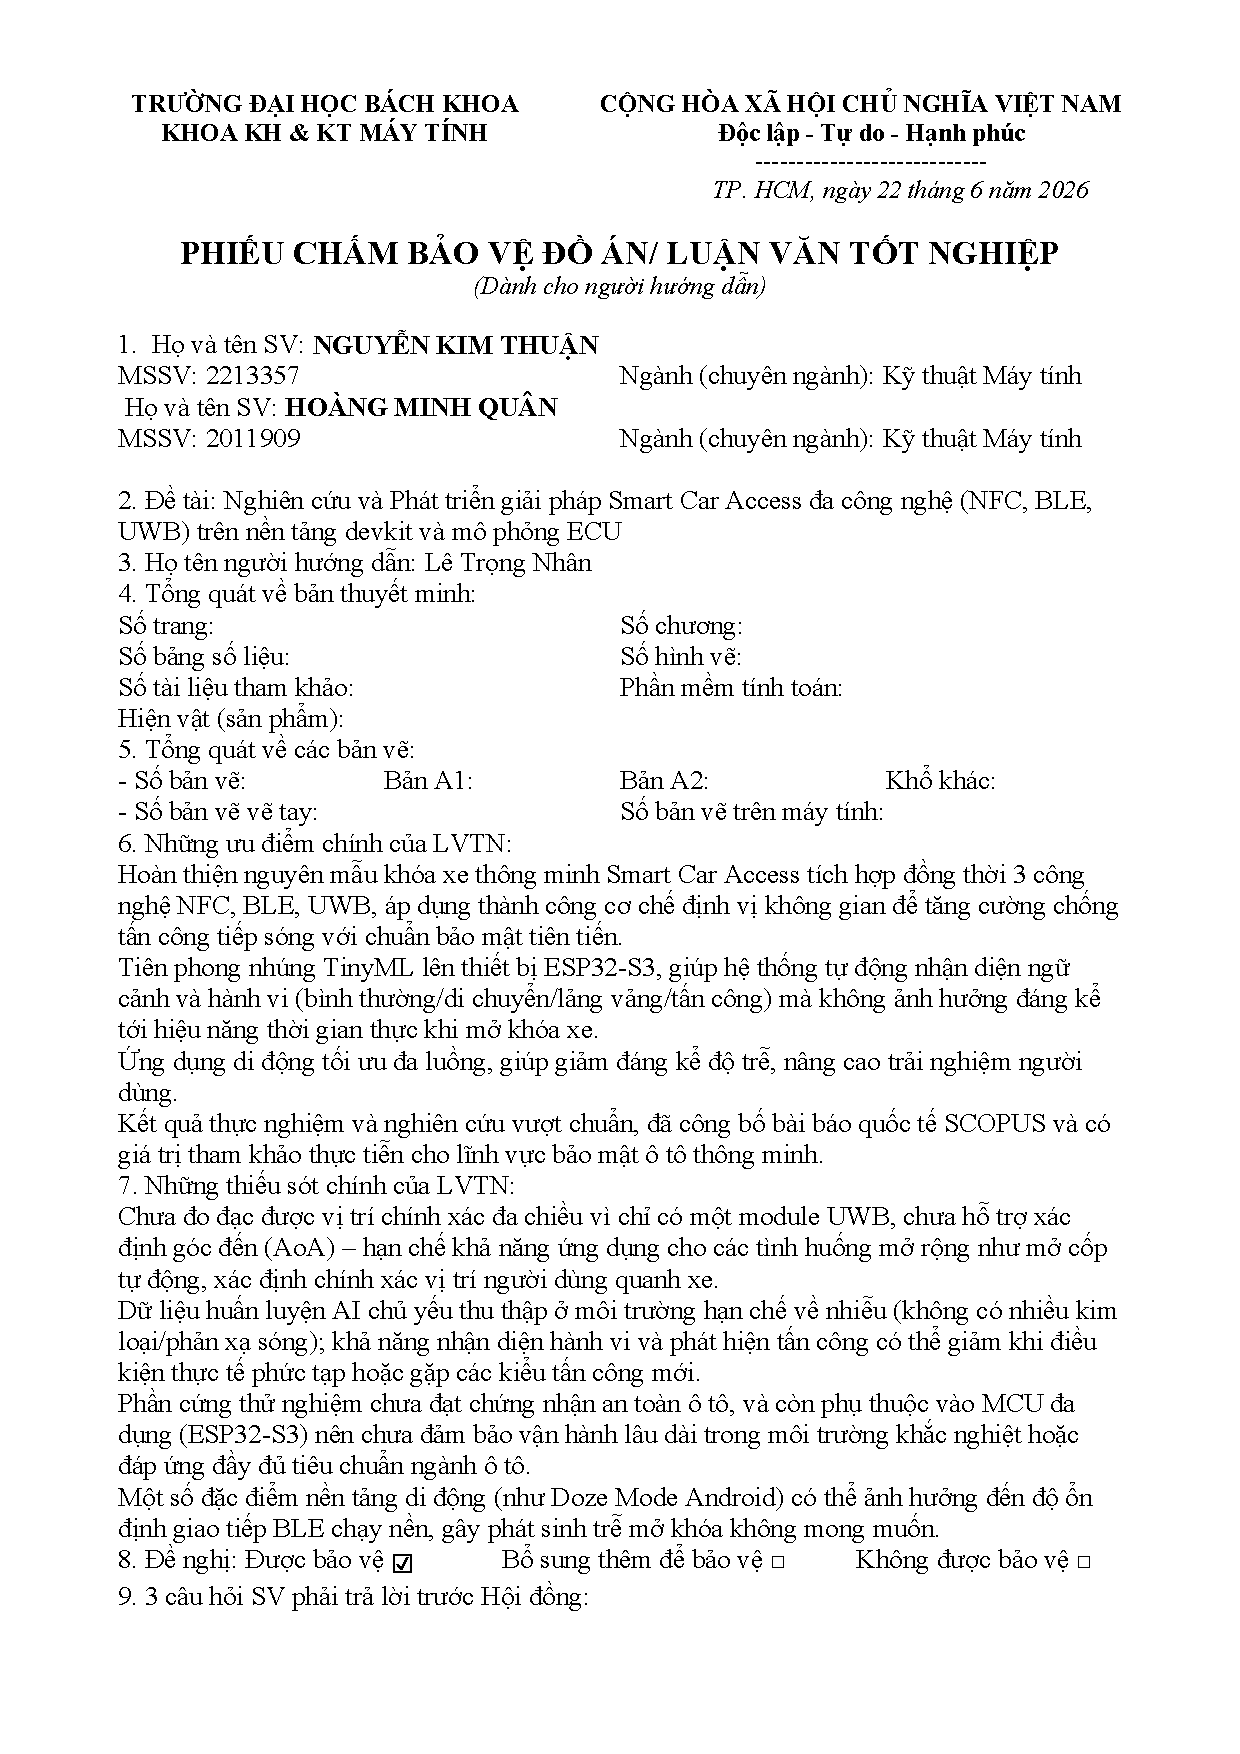
\includepdf[pages=1,pagecommand={},width=\paperwidth,height=\paperheight]{pdf files/Hd_signed.pdf}


% \newpage
% \thispagestyle{empty}
% \mbox{}
% \newpage

% 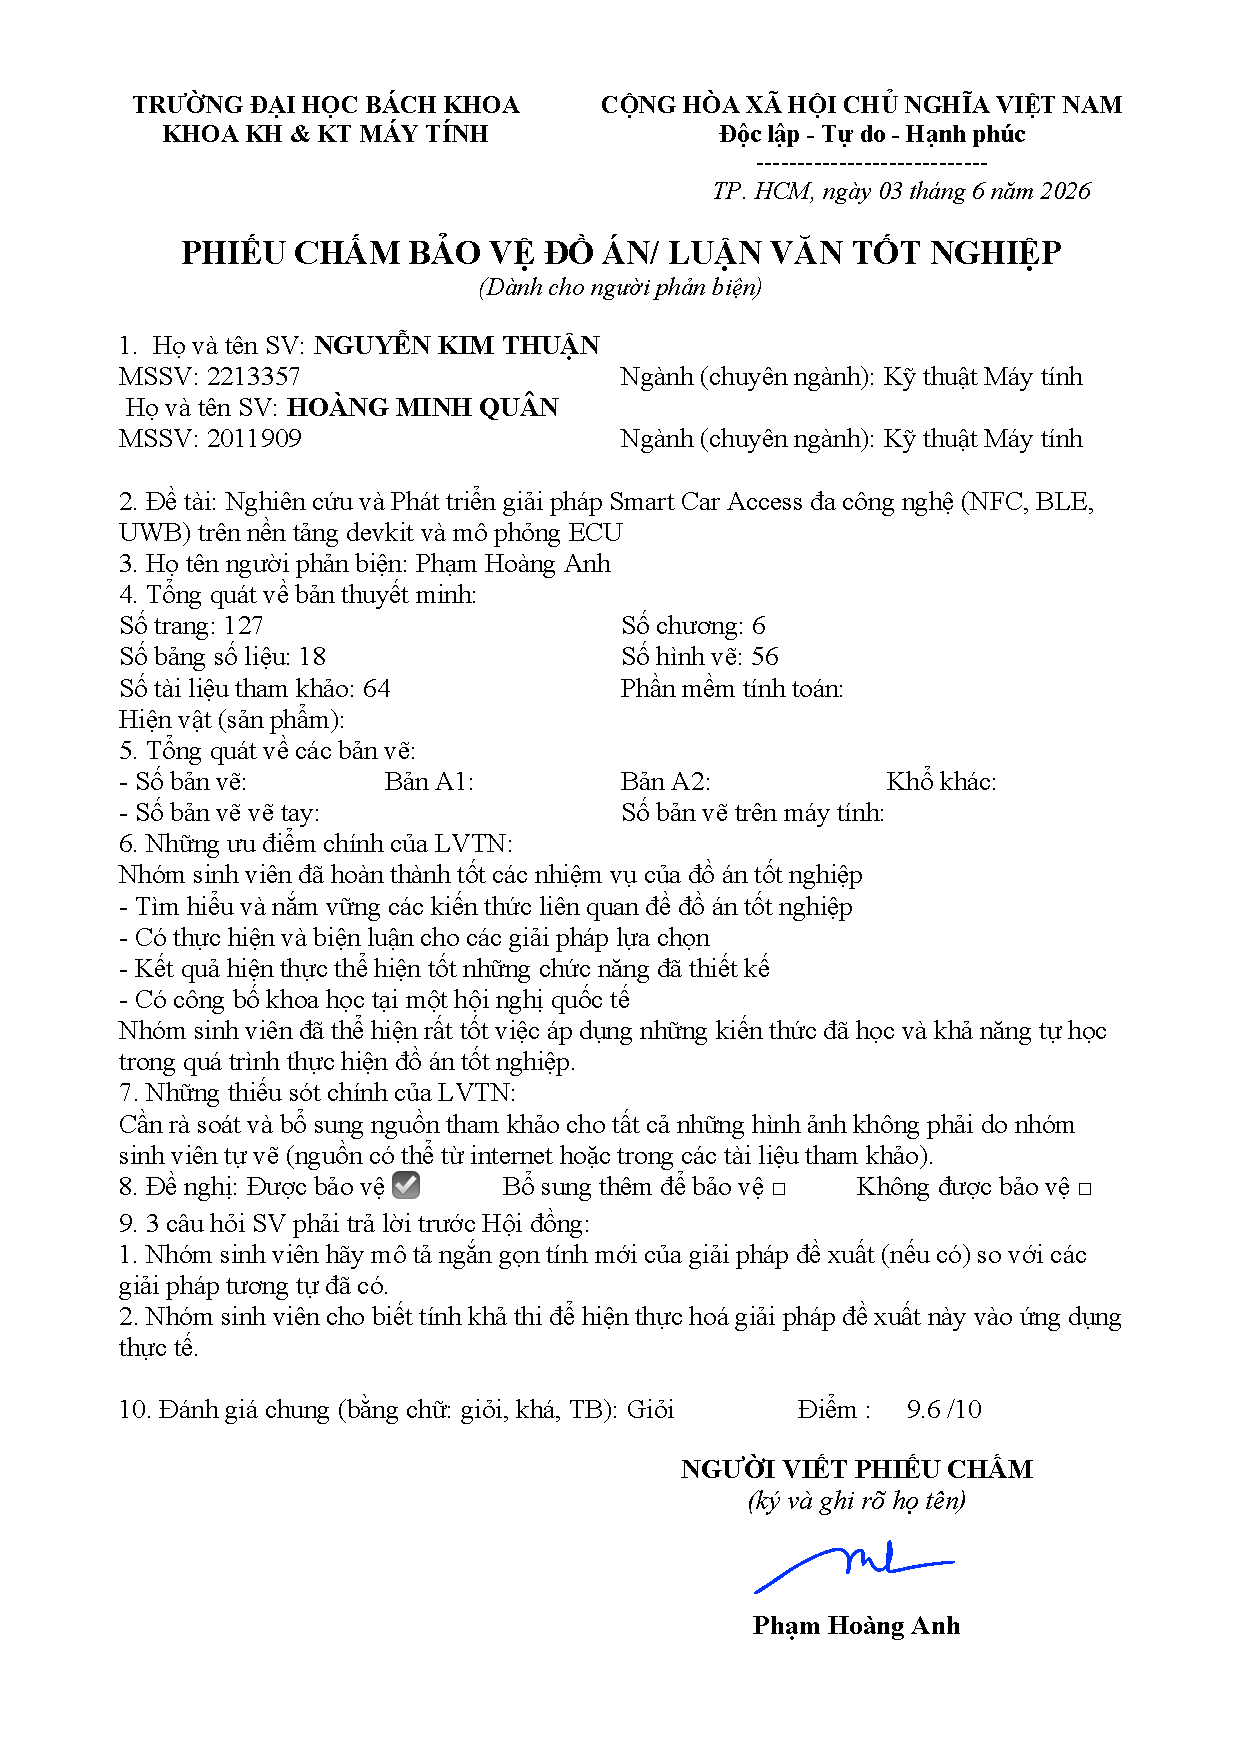
\includepdf[pages=1,pagecommand={},width=\paperwidth,height=\paperheight]{pdf files/PB_signed.pdf}


% \newpage
% \thispagestyle{empty}
% \mbox{}
% \newpage



\end{document}
